              %=================================================================%
              %                                                                 %
              %         Adapted from a thesis model by Lorenzo Pantieri         %
              %                       Alessandro Candido                        %
              %                                                                 %
              %=================================================================%
       
% !TeX program = pdflatex

\documentclass[10pt,%                      % corpo del font principale
               b5paper,%                   % carta A4
               twoside,openright,%         % fronte-retro
%              oneside,openany,%           % solo fronte
               titlepage,%                 % frontespizio
               headinclude,,footinclude,%  % testatina e piede di pagina
               cleardoublepage=empty,%     % pagine vuote senza testatina e piede di pagina
               captions=tableheading,%     % didascalie in cima alle tabelle
               ]{scrbook}                  % book class of KOMA-Script;
               
% packages and style
% !TEX encoding = UTF-8
% !TEX root = ../thesis.tex

% font encoding:
% NOTA BENE! richiede una distribuzione *completa* di LaTeX,
% per esempio TeXLive o MiKTeX *complete*
\usepackage[T1]{fontenc}

% input encoding:
% [latin1] is also fine
% ACHTUNG! Sync to editor preferences
\usepackage[utf8]{inputenc}

% to write both in Italian and English;
% last language is the default one
\usepackage[italian,english]{babel}

% images
\usepackage{graphicx}

% quotes
\usepackage[font=small]{quoting}

% math
\usepackage{amsmath,amssymb,amsthm}

% complete page references
\usepackage[english]{varioref}

% fixed width tables
\usepackage{tabularx}

% double quotes optimized for biblatex
\usepackage[autostyle,italian=guillemets]{csquotes}

% bibliography;
% make citing style author-year;
% the style "numeric-comp" makes numeric references;
\usepackage[style=philosophy-modern, url=false,
			hyperref,square,backend=biber]{biblatex}

% biblatex database
\addbibresource{library.bib}

% sub-figures and sub-tables
\usepackage{subfig}

% pseudo-text
\usepackage{lipsum}

% ClassicThesis style
% - chapter numbers in Euler font
% - if using subfig package
% - Bera Mono as monospace font
% - AMS Euler as math font
% - improve line spacing
% - codes
% - for documents divided in parts 
\usepackage[eulerchapternumbers,%
            subfig,%
            beramono,%
            eulermath,%
            pdfspacing,%
            listings,%
            parts,%
            ]{classicthesis}
% rearrange the appearance of classicthesis
\usepackage{arsclassica}

\newlength{\myshift}
\setlength{\myshift}{4mm}
\addtolength{\evensidemargin}{-\myshift}
\addtolength{\oddsidemargin}{\myshift}
%\setlength{\evensidemargin}{8.40024mm} % initial value: 12.40024mm
%\setlength{\oddsidemargin}{3.80026mm} % initial value: -0.19974mm

\usepackage{datetime2}
\usepackage{datetime2-calc}
\usepackage{ifthen}
\usepackage{etoolbox}
\usepackage{calc}
\usepackage[sort]{cleveref}

% glossaries (after hyperref)
\usepackage[acronym,automake,nomain,section=section]{glossaries}
%\newglossary*{sym}{Symbols}
\newglossary*{symbols}{Symbols}
\renewcommand*{\glstextformat}[1]{\textcolor{CTurl!30!black}{#1}} %color defined by classichthesis
\makeglossaries

\usepackage{ifoddpage}
% !TeX root = ../main.tex

% manage layouts
\usepackage{geometry}

% indent first paragraph of each section
\usepackage{indentfirst}

% fixed width tables
% \usepackage{tabularx}

\usepackage{booktabs}
\usepackage{subfig}
\usepackage[bottom]{footmisc}
\usepackage{float}
%\usepackage[bottom]{footmisc}		% note a fondo pagina
%\usepackage{emptypage}
\usepackage{verbatim}
\usepackage{lipsum}
\usepackage{enumerate}
%\usepackage{enumitem}
\usepackage{changepage}
\let\checkmark\relax
\usepackage{dingbat}
\usepackage{lettrine}

%*********************************************************************************
% Color Boxes
%*********************************************************************************
%\usepackage{layouts}
%\printinunitsof{mm}{\pagevalues}
%\verb|\marginparwidth|: \printinunitsof{mm}\prntlen{\marginparwidth}

%*********************************************************************************
% Tikz
%*********************************************************************************
\usepackage{pgf}
\usepackage{tikz}
\usepackage{rotating}
\usepackage{pgfornament}
% \usepackage{pgfornament,pgfornament-han}
\usetikzlibrary{arrows,shapes,decorations,automata,backgrounds,petri,positioning}

\setlength{\skip\footins}{15pt}

%*********************************************************************************
% Color Boxes
%*********************************************************************************

\usepackage{tcolorbox}
\tcbuselibrary{theorems}

%*********************************************************************************
% Optimized margins for B5
%*********************************************************************************
\KOMAoptions{BCOR=10mm}
\areaset[current]{360pt}{650pt}
\setlength{\marginparwidth}{7em}
\setlength{\marginparsep}{2em}%

%*********************************************************************************
% Minitoc settings
%*********************************************************************************
\usepackage{minitoc}
\dominitoc[e]
\mtcsetrules{minitoc}{off}
\mtcsetfeature{minitoc}{before}{\textcolor{black!70}{\rule{0.8\textwidth}{0.1pt}}\vspace{-20pt}}
\mtcsetfeature{minitoc}{after}{\vspace{-20pt}\textcolor{black!70}{\rule{0.8\textwidth}{0.1pt}}}
\setcounter{tocdepth}{2}

%*********************************************************************************
% listings settings - code snippets
%*********************************************************************************
\usepackage{listings}
\lstset{language=[LaTeX]Tex,%C++,
    keywordstyle=\color{RoyalBlue},%\bfseries,
    basicstyle=\small\ttfamily,
    %identifierstyle=\color{NavyBlue},
    commentstyle=\color{Green}\ttfamily,
    stringstyle=\rmfamily,
    numbers=none,%left,%
    numberstyle=\scriptsize,%\tiny
    stepnumber=5,
    numbersep=8pt,
    showstringspaces=false,
    breaklines=true,
    frameround=ftff,
    frame=single
} 

% !TeX root = ../main.tex

% --- PACKAGES ---
\usepackage{mathtools,physics,tensor}
\usepackage{bbold,mathrsfs}
\usepackage{bm}
\usepackage{slashed}
%\usepackage[mathscr]{euscript}
%\usepackage{bickham}		% redefines \mathcal e \mathbcal
							% al momento non riesco a farlo funzionare
%\usepackage{mathalfa}		% powerful package with a lot of math fonts
%\usepackage{fourier}		% alternativa decente a bassa sbatta
%\usepackage[euler-digits,euler-hat-accent]{eulervm}
\usepackage[cdot, thickqspace, squaren]{SIunits}
% ------------

% --- THEOREMS ---
% theorems (with amsthm) in english
\theoremstyle{plain}% default
\newtheorem{thm}{Theorem}[section]
\newtheorem{lem}[thm]{Lemma}
\newtheorem{prop}[thm]{Proposition}
\newtheorem*{thm*}{Theorem}
\newtheorem*{lem*}{Lemma}
\newtheorem*{prop*}{Proposition}
\newtheorem*{cor}{Corollary}

\theoremstyle{definition}
\newtheorem{defn}{Definition}[section]
\newtheorem{es}{Example}[section]
\newtheorem{ex}{Exercise}[section]
\newtheorem*{defn*}{Definition}
\newtheorem*{es*}{Example}
\newtheorem*{ex*}{Exercise}
\newtheorem*{note}{Note}

% ENVIRONMENTS
\newtcbtheorem[number within=section]{example}{Example}%
{colback=CornflowerBlue!4,colframe=CornflowerBlue!60!black,fonttitle=\bfseries,before upper={\parindent15pt\noindent}}{th}

%\newtcbtheorem[number within=section]{mytheo}{My Theorem}%
%{colback=green!5,colframe=green!35!black,fonttitle=\bfseries}{th}
% ------------


% mycommands
\newcommand{\ttmp}[1]{\textit{\textcolor{violet}{#1}}}
\newcommand{\gsym}[1]{\glssymbol{#1}}

%\newcommand{\Section}[2][]{
%	\ifstrempty{#1}{%
%		\section{#2}
%	}{%
%		\setcounter{section}{#1-1}
%		\section{#2}
%	}%
%}

% personal settings
% Here are stored personal settings

%*********************************************************************************
% Personal commands
%*********************************************************************************
% author
\newcommand{\myName}{Alessandro Candido}                        
% title
\newcommand{\myTitle}{Theory Predictions for PDF fitting}
% thesis type
\newcommand{\myDegree}{PhD Thesis}                          
% university
\newcommand{\myUni}{Universit\`a degli Studi di Milano}       					
% department
\newcommand{\myDepartment}{Dipartimento di Fisica Aldo Pontremoli}      
% supervisor
\newcommand{\myProf}{Prof.~Stefano Forte}             		
% co-supervisor
\newcommand{\myOtherProf}{Prof.~Stefano Carrazza}        
% where
\newcommand{\myLocation}{Milan}                                  
% when
\newcommand{\myTime}{\DTMMonthname{\the\month} \the\year}       

%*********************************************************************************
% amsmath, amssymb, amsthm settings
%*********************************************************************************

% theorem, laws, and acts (amsthm package required)
\theoremstyle{plain} 
\newtheorem{theorem}{Theorem}
\newtheorem{law}{Law}
\newtheorem{act}[law]{Act}
\newtheorem{murphy}{Murphy}[section]

%*********************************************************************************
% biblatex settings
%*********************************************************************************
\defbibheading{bibliography}{%
\cleardoublepage
\manualmark
\phantomsection 
\addcontentsline{toc}{chapter}{\tocEntry{\bibname}}
\chapter*{\bibname\markboth{\spacedlowsmallcaps{\bibname}}
{\spacedlowsmallcaps{\bibname}}}}

%*********************************************************************************
% listings settings
%*********************************************************************************
\lstset{language=[LaTeX]Tex,%C++,
    keywordstyle=\color{RoyalBlue},%\bfseries,
    basicstyle=\small\ttfamily,
    %identifierstyle=\color{NavyBlue},
    commentstyle=\color{Green}\ttfamily,
    stringstyle=\rmfamily,
    numbers=none,%left,%
    numberstyle=\scriptsize,%\tiny
    stepnumber=5,
    numbersep=8pt,
    showstringspaces=false,
    breaklines=true,
    frameround=ftff,
    frame=single
} 

%*********************************************************************************
% graphicx settings
%*********************************************************************************
\graphicspath{{pictures/}}

%*********************************************************************************
% Optimized margins for A4
%*********************************************************************************
\areaset[current]{370pt}{750pt}
\setlength{\marginparwidth}{7em}
\setlength{\marginparsep}{2em}%

%*********************************************************************************
% varioref settings
%*********************************************************************************
\makeatletter
\vref@addto\extrasitalian{%
   \def\reftextfaraway#1{a pagina~\pageref{#1}}%
}
\makeatother

%*********************************************************************************
% More
%*********************************************************************************

% [...] ;-)
\newcommand{\omissis}{[\dots\negthinspace]}

% hyphenation exceptions
\hyphenation{Fortran ma-cro-istru-zio-ne nitro-idrossil-amminico}

% correct scrreprt's bug about figure numbering
\renewcommand*{\figureformat}{%
  \figurename~\thefigure%
  %\autodot%
}
\renewcommand*{\tableformat}{%
  \tablename~\thetable%
  %\autodot%
}


\begin{document}
    \pagestyle{scrheadings}

    %******************************************************************
    % Front Matter
    %******************************************************************
    % !TeX root = ../../main.tex

\pdfbookmark{Cover}{Cover}
\newgeometry{width=370pt,height=650pt,centering}

\begin{center}
	
\includegraphics[width=11cm]{logo-unimi}
	\vspace*{10pt}

	Scuola di Dottorato in Fisica, Astrofisica e Fisica Applicata\\
	\myDepartment\\
	\vspace*{5pt}
	\textbf{Ciclo XXXV}

	\vfill

	{\Huge \myTitle}\\
	\vspace*{30pt}
	\textit{Settore Scientifico Disciplinare FIS/02}\\

	\vfill

	\textbf{Supervisor:} \hfill \textbf{Candidate:}\\
	\myProf \hfill \myName\\
	\vspace*{15pt}
	Anno Accademico 2021/2022
\end{center}
	
	
\pagenumbering{gobble}

\cleardoublepage
\restoregeometry
 
    \pagenumbering{roman}
    % % !TEX encoding = UTF-8
% !TEX root = ../../main.tex
% !TEX spellcheck = en-US

%*******************************************************
% Frontespizio
%*******************************************************
	
\thispagestyle{empty}
\phantomsection
\pdfbookmark{Title Page}{Title Page}

\begin{center}
	{\huge \textsf{\myTitle}}\\
	\vspace{5pt}
	{\large \textsf{\myName}}
\end{center}

\vspace*{4cm}

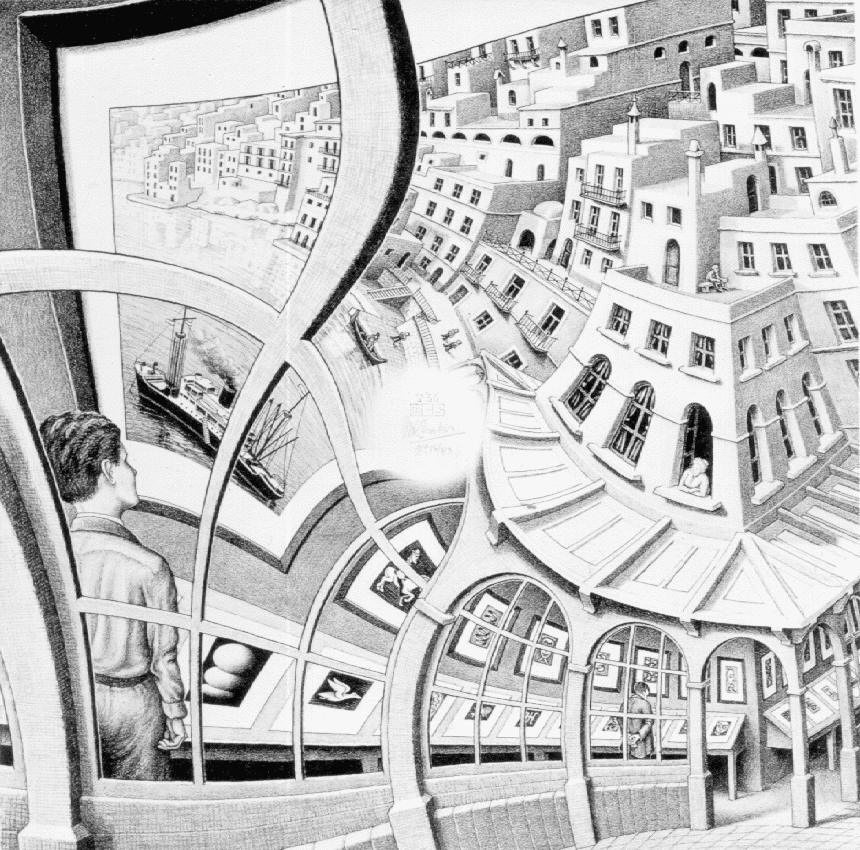
\includegraphics[width=\textwidth]{galleria-stampe}

    % !TEX encoding = UTF-8
% !TEX root = ../../main.tex
% !TEX spellcheck = en-US

%*******************************************************
% Colophon
%*******************************************************
\clearpage
\phantomsection
\thispagestyle{empty}

\hfill

\vfill

%\noindent\myName: \textit{\myTitle,}
%\myDegree,
%\textcopyright\ \MakeTextLowercase{\myTime}.

\noindent\spacedlowsmallcaps{Colophon}\rmfamily\\
%\noindent \MakeTextLowercase{\sffamily\scshape{\textsc{Colophon}}}\\
This thesis is written using \textit{ArsClassica} by Lorenzo Pantieri, a style
based on the original \LaTeX~package \textit{classicthesis} of André Miede,
inspired by Robert Bringhurst’s work \textit{“The Elements of Typographic
Style”}.
\newline

% \noindent On previous page is reproduced \textit{Print Gallery} by M. C.
% Escher, 1956 (this and other works of Escher are shown at
% \href{http://www.mcescher.com/}{http://www.mcescher.com/}).
% \vspace*{15pt}

\noindent\spacedlowsmallcaps{Contacts}\rmfamily\\
\leftpointright	 \href{mailto:\myEmail}{\myEmail}
$\cdot$ Write to \myName

    % !TEX encoding = UTF-8
% !TEX root = ../../main.tex
% !TEX spellcheck = it-IT

%*******************************************************
% Dedica
%*******************************************************
\cleardoublepage
\phantomsection
\thispagestyle{empty}
\pdfbookmark{Dedication}{Dedication}

\vspace*{3cm}

\begin{center}
felix qui potuit rerum cognoscere causas [...]\\
fortunatus et ille deos qui nouit agrestis \\ \medskip
--- P. Vergilius Maro, \textit{Georgicon}
\end{center}

\medskip

\begin{center}
	Dedicato al mio dottorato.
\end{center}

    % !TEX encoding = UTF-8
% !TEX root = ../../main.tex
% !TEX spellcheck = en-US

%*******************************************************
% Indici
%*******************************************************
\cleardoublepage
\pdfbookmark{\contentsname}{tableofcontents}
\dominitoc[e]
\mtcsetrules{minitoc}{off}
\mtcsetfeature{minitoc}{before}{\hspace*{-10pt}\textcolor{black!70}{\rule{\textwidth}{0.1pt}}\vspace{-30pt}}
\mtcsetfeature{minitoc}{after}{\vspace{-20pt}\hspace*{-10pt}\textcolor{black!70}{\rule{\textwidth}{0.1pt}}}
\setcounter{tocdepth}{2}
\tableofcontents
\adjustmtc
\markboth{\spacedlowsmallcaps{\contentsname}}{\spacedlowsmallcaps{\contentsname}} 
\clearpage

\begingroup 
    \let\clearpage\relax
    \let\cleardoublepage\relax
    %*******************************************************
    % Elenco delle figure
    %*******************************************************    
    \phantomsection
    \pdfbookmark{\listfigurename}{lof}
    \listoffigures

    \vspace*{5cm}

    %*******************************************************
    % Elenco delle tabelle
    %*******************************************************
    \phantomsection
    \pdfbookmark{\listtablename}{lot}
    \listoftables
       
\endgroup
\vfill

%\pagebreak
%\phantomsection
%\pdfbookmark{Sommario}{Sommario}
%\begingroup
%\let\clearpage\relax
%\let\cleardoublepage\relax
%\let\cleardoublepage\relax
%
%\ttmp{Se qui rimane una pagina bianca posso metterci un breve sommario}

%\chapter*{Sommario}
%
%\lipsum[1]
%
%\vfill

%\vspace*{100pt}

%\selectlanguage{english}
%\pdfbookmark{Abstract}{Abstract}
%\chapter*{Abstract}
%
%\lipsum[2]
%
%\selectlanguage{italian}
%
%\endgroup			

\cleardoublepage

    %We discuss the sensitivity of theoretical predictions of observables used in
searches for new physics to parton
distributions (\pdfs) at large momentum fraction $x$.
%
Specifically, we consider the neutral-current \acrlong{dy} production of
gauge bosons with invariant masses in the TeV range, for which    
the forward-backward asymmetry of charged leptons
from the decay of the gauge boson in its rest frame is a traditional
probe of new physics. We show that the qualitative  behaviour of the asymmetry 
depends strongly on the assumptions made in determining the underlying \pdfs.
%
 We discuss and compare the large-$x$
 behaviour of various different \pdf sets, and find that they 
 differ significantly.
 %
 Consequently, the shape of the asymmetry observed at lower
 dilepton invariant masses, where all \pdf sets are in reasonable agreement 
because of  the presence of experimental constraints,
 is not necessarily reproduced at large masses where the
 \pdfs are mostly unconstrained by data.
%
 It follows that the shape 
of the asymmetry at high masses may depend on 
assumptions made in the \pdf parametrization, 
and thus deviations from the traditionally expected behaviour cannot be taken as a reliable 
indication of new physics.
%
We demonstrate that forward-backward asymmetry measurements
could help in constraining \pdfs at large $x$ and discuss the accuracy that would be required to
disentangle the effects of new physics from uncertainties in the \pdfs in this region.

    % !TeX root = ../../../main.tex

Software has been central in \acrlong{hep} since many years

\hep needs and deserves reliable and maintainable software, i.e.\ not dead or
frozen, but living and evolving according to the needs of the field.

There is limited manpower available to write software.
Therefore, this has to be compensate by good designs and architectures, and to
do that is appropriate concert development planning with all the relevant
stakeholders.


    \cleardoublepage

    %******************************************************************
    % Main Matter
    %******************************************************************
    \pagenumbering{arabic}
    \part{Theory}
    % !TeX root = ../../../main.tex

%************************************************
\chapter{Forward-Backward Asymmetry}
\label{ch:afb}
%************************************************
\minitoc
\adjustmtc


% !TeX root = ../../../main.tex

The first fundamental application of the integrated pineline will actually the
inclusion of \acrfull{mhou} at \nnlo in the \nnpdfr{4.0} fit.

\pdfs are non-perturbative objects, so it may seem counter-intuitive that their
accuracy depends on perturbative series truncation.
%
This is a direct consequence of extracting them from high energy collisions
data: they are completely determined by physics that happens in the
perturbative regime, and the map discussed at the beginning of this chapter
(the one that connects data to \pdfs) is completely determined by \pqft
calculations.
%
So, the origin of the perturbative order of \pdf sets is exactly determined by
the theory predictions used during the extraction: a \nnlo set is a \pdf set
that has been fitted using theory predictions at \nnlo.
%
A \pdf set directly computed with non-perturbative methods would have no
perturbative order associated, even when used in a perturbative calculation
\footnote{
	From that point of view would be an \textit{all-order} object, even though
	it might be subject to other kinds of approximations.
}\footnote{
	Also consider that \dglap evolution is perturbative, so, once evolved, it
	acquires again a dependency on the perturbative truncation.
}.

The perturbative series enters in the \pdf in two different places: the
partonic cross section calculations (those encoded in \textit{grids}) and the
\dglap evolution\footnote{
	That technically is used twice: during the fit, to bridge data with the
	boundary condition candidate, and to evolve the final boundary condition to
	all scales.
	But considering the \pdf a function of two variables ($z$ and $\mu_F^2$)
	consistently, the abstract evolution flow used is a single one.
}.
%
In principle, these are two different perturbative orders, thus there is not a
single truncation, but two of them, and they can happen at two different
orders.
%
Still, the two objects are not completely decoupled: \dglap evolution arise
from collinear divergences, subtracted by the chosen factorization scheme.
These collinear logarithms appear as well in the partonic cross sections, so it
is important to properly account for them, avoiding double counting.
%
The whole picture of collinear subtractions is deeply connected to treatment of
quark masses, better discussed in \cref{ch:dis}, since a finite value of the
mass regulates the collinear divergence on its own.
%
Therefore, the double perturbative order already appears in the partonic cross
sections calculations, where the \fns chosen can account for light and heavy
quarks at two distinct orders (cf. \cite{Forte:2010ta}, in particular the
FONLL-B scheme).


\section{Anatomy of Drell-Yan production}
\label{sec:afb/HMDY}
% !TeX root = ../../../main.tex

The aim of this  section is to scrutinize the \pdf dependence of the
neutral-current \acrlong{dy} differential cross-section and of the associated
forward-backward asymmetry by reviewing the \lo kinematics, determining \lo
analytic expressions, and finally comparing these analytical calculations to
the results of \lo and \nlo  numerical simulations obtained using \mgamc,
\cite{Alwall:2014hca}, interfaced to \pineappl,
\cite{Carrazza:2020gss,christopher_schwan_2022_7023438}.
%
Specifically, we will relate the behavior of the differential distribution and
asymmetry to the relevant parton luminosities.

\subsection{Drell-Yan kinematics and cross-sections at \lo}
\label{sec:dylo}

We consider dilepton production via the exchange of an electroweak neutral
gauge boson $Z/\gamma^*$ in proton-proton collisions:
\begin{equation}
  \label{eq:DYprocess}
  \mathrm{p}(k_1) + \mathrm{p}(k_2) \to Z/\gamma^*(q) \to \ell(p_{\ell}) + \bar{\ell}(p_{\bar{\ell}}) + X \text{.}
\end{equation}
The hadronic differential cross-section $\dd\sigma^{\mathrm{p}\mathrm{p}\to\llb}$  is factorized in
terms of \pdfs $f_i$ and the partonic cross sections
$\dd\hat\sigma_{ij}$ for incoming partons of species $i,\,j$ as
\begin{equation}
  \dd\sigma^{\mathrm{p}\mathrm{p}\to\llb} = \sum_{ij} \int\limits_0^1\!\dd x_1 \dd
  x_2 f_i(x_1,\mu_F^2) f_j(x_2,\mu_F^2) \dd\hat\sigma_{ij}(\hat k_1 = x_1
  k_1, \hat k_2 = x_2 k_2).
  \label{eq:factorization}
\end{equation}
In the sequel we will set the  factorization scale $\mu_F$ to the
invariant mass of the gauge boson, i.e.\ the dilepton
invariant mass, so $\mu^2_F = \mll^2=(p_\ell + p_{\bar{\ell}})^2$.
%
The kinematics and Feynman diagram of the \lo partonic process
in the quark-antiquark channel are shown in \cref{fig:lo-dy}.
We do not consider photon-initiated processes, as they do not affect
the qualitative features of our discussion.

%--------------------------------------
\begin{figure}[t]
  \centering

  \begin{tikzpicture}
    \begin{feynman}
      \tikzfeynmanset{large}

      \vertex (b);
      \vertex [above left=of b] (a) {\(q\)};
      \vertex [below left=of b] (f1) {\(\bar{q}\)};
      \vertex [right=of b] (c);
      \vertex [above right=of c] (f2) {\(\ell\)};
      \vertex [below right=of c] (f3) {\(\bar{\ell}\)};

      \diagram* {
      (a) -- [fermion, momentum=\(\hat{k}_1\)] (b) -- [fermion, rmomentum=\(\hat{k}_2\)] (f1),
      (b) -- [boson, edge label'=\(\gamma / Z\), momentum=\(q\)] (c),
      (c) -- [anti fermion, momentum=\(p_{\ell}\)] (f2),
      (c) -- [fermion, momentum=\(p_{\bar{\ell}}\)] (f3),
      };
    \end{feynman}
  \end{tikzpicture}

  \caption{Neutral-current Drell-Yan production at \lo in the quark-antiquark channel.}
  \label{fig:afb/lo-dy}
\end{figure}

%--------------------------------------

At \lo, the momentum fractions of the two incoming partons are fully
fixed by knowledge of the invariant mass and rapidity of the gauge
boson, i.e.\ of the dilepton pair  $\yll = (y_\ell + y_{\bar{\ell}})/2$: 
\begin{equation}
  \label{eq:x_fractions}
  x_1 = \frac{ \mll}{\sqrt{s}}\exp(\yll) \, ,\quad x_2 = \frac{
  \mll}{\sqrt{s}}\exp(-\yll) \, ,
\end{equation}
where the center of mass energy of the hadronic collision is
$s=(k_1+k_2)^2$ and at \lo
$\mll^2 = \hat s = x_1 x_2 s$. The absolute dilepton
rapidity thus lies in the range $|\yll|\le \ln (\sqrt{s}/\mll)$.
Beyond \lo there might be extra radiation in the final state, so the \lo
kinematics provides a lower bound on the momentum fractions of the
incoming partons, and all values of the momentum
fractions such that $x_{1,2}\ge \mll/\sqrt s$ are allowed.

It is useful to define the so-called  Collins-Soper
angle $\theta^*$~\cite{Collins:1977iv}, which in the hadronic \acrfull{com}
frame is defined as
\begin{equation}
\begin{split}
  \cos\theta^* &= \sign (\yll) \cos\theta \, ,\\
  \cos\theta &\equiv\frac{p_\ell^+ p_{\bar{\ell}}^- - p_\ell^- p_{\bar{\ell}}^+}{\mll \sqrt{\mll^2 + p_{\mathrm{T},\ell\bar{\ell}}^2}} \text{,} \quad p^\pm = p^0 \pm p^3 \text{.}
  \label{eq:cosine-cs-angle}
\end{split}
\end{equation}
It is easy to show that the Collins-Soper angle $\theta^*$ coincides with the
scattering angle of the lepton in the partonic \com frame, $\bar\theta$.
%
The latter is defined in terms of the lepton momentum as 
\begin{equation}
 \cos\bar\theta \equiv \frac{p^z_\ell}{\mll} \,, \label{eq:coscm}
\end{equation}
where the $z$ axis is along the direction of the incoming quark-antiquark pair.
%
In the partonic \com frame, of course, $p^z_\ell=-p^z_{\bar \ell}$ and $\yll
=0$, so
\begin{equation}
p^\pm_\ell=p^{\mp}_{\bar{\ell}}=  \mll \left( 1\pm \cos{\bar\theta} \right)\, ,
\end{equation}
and substituting in \cref{eq:cosine-cs-angle} it immediately follows that,
taking the convention 
$\sign (\yll)=\sign(0)=+1$, 
$\cos\theta^*=\cos\theta=\cos{\bar\theta}$.
%
The expression of $\cos\theta$ in \cref{eq:cosine-cs-angle} is manifestly
invariant upon boosts along the $z$ axis, so the identification of $\theta$
with the \com scattering angle $\bar\theta$ remains true in any reference
frame.

Note that the definition \cref{eq:coscm} requires a choice for the positive
direction of the $z$ axis, which is usually taken along the direction of the
incoming fermion (quark).
%
This direction is  not experimentally accessible in proton-proton collisions,
so the Collins-Soper angle is defined by always taking the positive $z$ axis in
the direction of the boosted dilepton pair, i.e., at \lo, along the direction of
the incoming quark with largest momentum fraction, i.e.\ by supplementing in
the definition a factor $\sign(\yll)$.
%
Hence $\cos\theta^*=\cos{\bar\theta}$ ($\cos\theta^*=-\cos{\bar\theta}$)  if
the momentum fraction of the incoming quark (antiquark) is the largest.

%
The hard scattering matrix elements that enter the partonic cross-section
in \cref{eq:factorization} are the sum of a pure photon-exchange
contribution, a photon-$Z$ interference term, and a pure $Z$-exchange
contribution.
%
Of course, in the region
$\mll \gtrsim m_Z$ these contributions are all of the same order.
%
Standard arguments~\cite{Peskin:1995ev} then imply that, because in the
Standard Model the photon
coupling to leptons is vector  while the $Z$ coupling is chiral,
the pure photon and pure $Z$ contributions to the cross-section are
necessarily  even in $\cos\theta^*$ while the interference term is
odd.

Specifically, at \lo the fully differential hadronic cross-section can
be obtained from the well-known result~\cite{Peskin:1995ev} for
$e^+e^-\to\mu^+\mu^-$ by replacing the incoming lepton charges  with
those of the quarks, and accounting for the \pdfs, with
the result
\begin{align}
    \frac{\dd^3 \sigma}{\dd \mll \, \dd \yll \, \dd\cos\theta^*} &= \frac{\pi \alpha^2}{3 \mll s} \left((1+\cos^2({\theta^*})) \sum_q S_q \left[f_q(x_1,\mll^2) f_{\bar{q}}(x_2,\mll^2) + f_q(x_2,\mll^2) f_{\bar{q}}(x_1,\mll^2) \right] \right. \nonumber\\
    &\hspace*{15pt} + \left. \cos\theta^* \sum_q A_q \sign (\yll) \left[ f_q(x_1,\mll^2) f_{\bar{q}}(x_2,\mll^2) - f_q(x_2,\mll^2) f_{\bar{q}}(x_1,\mll^2)\right] \right) \, ,
    \label{eq:lo-triple-diff}
\end{align}
where  $\alpha$ is the QED coupling and the even (symmetric) and
odd  (antisymmetric) couplings are given by
\begin{align}
  \label{eq:coup}
    S_q &= e_l^2 e_q^2 + P_{\gamma Z} \cdot  e_l v_l e_q v_q + P_{ZZ} \cdot  (v_l^2+a_l^2)(v_q^2+a_q^2) \nonumber \\
    A_q &= P_{\gamma Z} \cdot 2 e_l a_l e_q a_q  + P_{ZZ} \cdot 8 v_l a_l  v_q a_q \, ,
\end{align}
in terms of the electric charges  $e_l$, $e_q$ and the vector and
axial couplings $v_l$, $v_q$ and $a_l$, $a_q$  of the leptons and
quarks, and the propagator factors
\begin{align}\label{eq:propgz}
    P_{\gamma Z}(\mll) &= \frac{2\mll^2 (\mll^2  - m_Z^2)}{\sin^2(\theta_W) \cos^2(\theta_W)\left[(\mll^2 - m_Z^2)^2 + \Gamma_Z^2 m_Z^2\right]}\\
\label{eq:propzz}
    P_{ZZ}(\mll) &= \frac{\mll^4}{\sin^4(\theta_W) \cos^4(\theta_W)\left[(\mll^2 - m_Z^2)^2 + \Gamma_Z^2 m_Z^2\right]},
\end{align}
with $m_Z$  and $\Gamma_Z$ respectively the $Z$ mass and width and $\theta_W$ the weak mixing angle.
%
In \cref{fig:lo-couplings} we display the
symmetric $S_q$ (left) and antisymmetric $A_q$ (right)
couplings, \cref{eq:coup}, for up-like and
down-like quarks, as a function of 
the dilepton invariant mass $\mll$.
%
Both couplings are around a factor 2 larger for
up-like quarks than for down-like quarks, and
become $\mll$-independent for $\mll \gsim 1$ TeV, where they take
the asymptotic values $\bar S_q$, $\bar A_q$ obtained by
substituting in \cref{eq:coup} the large-mass expressions of
the propagator factors
\begin{equation}\label{eq:propasympt}
    \bar P_{\gamma Z} = \frac{2}{\sin^2(\theta_W)\cos^2(\theta_W)},
    \qquad 
    \bar P_{ZZ} = \frac{1}{\sin^4(\theta_W) \cos^4(\theta_W)},
\end{equation}
to which $P_{\gamma Z}$ and $P_{ZZ}$ respectively reduce up to $O(m^2_Z/\mll^2)$ corrections.

 
%%%%%%%%%%%%%%%%%%%%%%%%%%%%%%%%%%%%%%%%%%%%%%%%%%%%
\begin{figure}
  \centering
  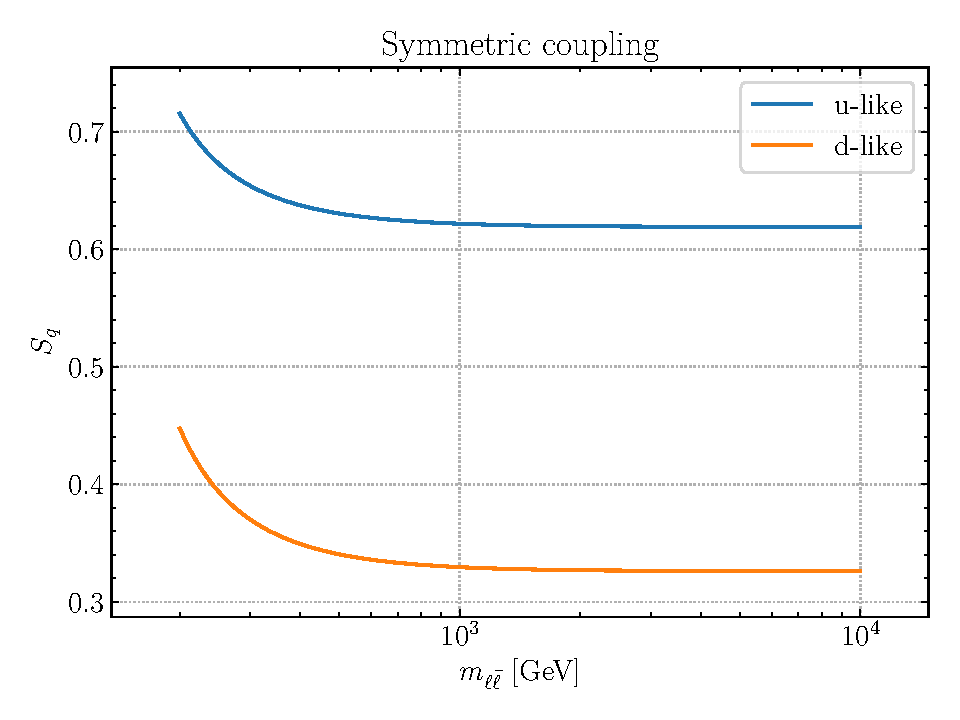
\includegraphics[width=0.49\linewidth]{ch-afb/symmetric-couplings.pdf}
  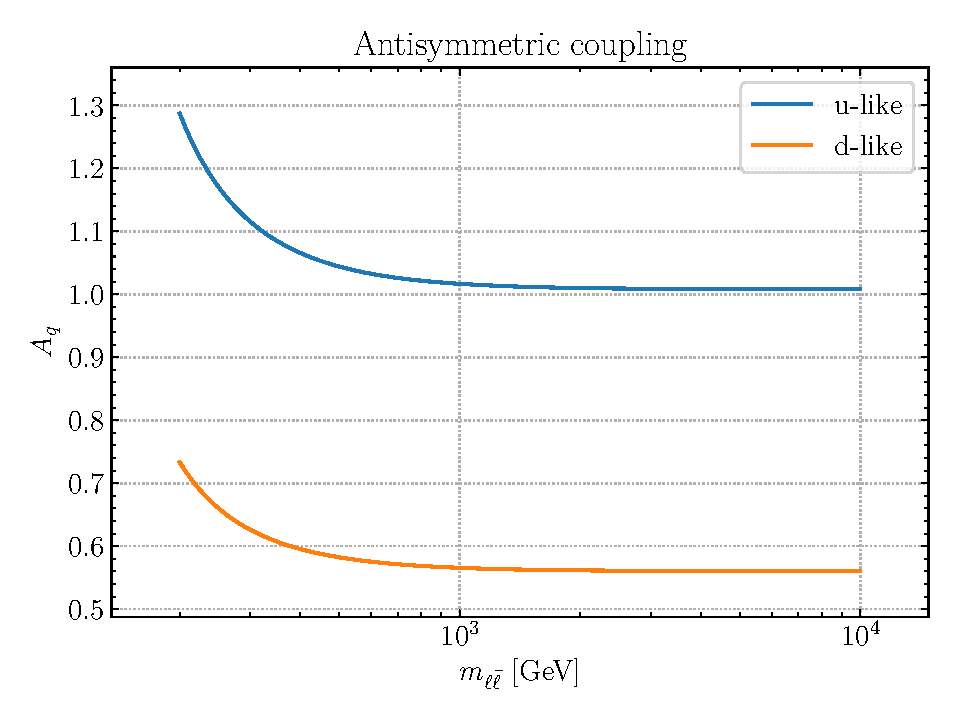
\includegraphics[width=0.49\linewidth]{ch-afb/antisymmetric-couplings.pdf}
  \caption{The symmetric $S_q$ (left) and antisymmetric $A_q$ (right)
    couplings, \cref{eq:coup}, for up-like and
    down-like quarks, as a function of 
 the dilepton invariant mass $\mll$.
  }
  \label{fig:lo-couplings}
\end{figure}
%%%%%%%%%%%%$$$$$$$$$$$$$$$$$$$$$%%%%%%%%%%%%%

The interference term proportional to
$A_q$ is odd in the Collins-Soper angle $\cos\theta^*$, leading to a forward-backward
scattering asymmetry.
%
In a proton-proton collision the initial state is completely
symmetric, so the quark and antiquark contributions to the
cross-section \cref{eq:lo-triple-diff} are necessarily symmetric
upon the interchange of the incoming quark and antiquark, with the
corresponding momentum fractions fixed at \lo by
\cref{eq:x_fractions}.
%
However, as mentioned, there
is a sign change in the relation between $\cos\theta^*$ and
$\cos\theta$ according to whether the incoming parton with largest
momentum fraction is a quark or an antiquark, i.e.,
when interchanging
$x_1$ with $x_2$ in the argument of the quark and antiquark \pdfs,
thereby leading to the result of  \cref{eq:lo-triple-diff}.
%
This leads
to a forward-backward asymmetry whenever the quark and antiquark
\pdfs have different $x$ dependence.

In order to understand the relation of this forward-backward
asymmetry in terms of the
behavior of the \pdfs, it is convenient
to rewrite the \pdf combinations that contribute to the differential
cross-section \cref{eq:lo-triple-diff} in terms of symmetric and
antisymmetric parton luminosities, defined as
\begin{align}
  \mathcal{L}_{S,q}(\mll, \yll) &\equiv f_q(x_1,\mll^2) f_{\bar{q}}(x_2,\mll^2) + f_q(x_2,\mll^2) f_{\bar{q}}(x_1,\mll^2) \, ,
  \nonumber\\
  \mathcal{L}_{A,q}(\mll, \yll) &\equiv \sign (\yll) \left[ f_q(x_1,\mll^2) f_{\bar{q}}(x_2,\mll^2) - f_q(x_2,\mll^2) f_{\bar{q}}(x_1,\mll^2)\right] \, , \label{eq:symm_asymm_lumis}
\end{align}
where the momentum fractions $x_1$ and $x_2$ are given in terms of $\mll$, $\yll$,
and $\sqrt{s}$ in \cref{eq:x_fractions}.
Note that both parton luminosities are invariant under
the interchange $x_1\leftrightarrow x_2$, upon which $\yll \to -\yll$.
%
In terms of these luminosities, the triple differential cross-section \cref{eq:lo-triple-diff}
takes the compact form
\begin{equation}
  \label{eq:lo-triple-diff-lumis}
  \frac{\dd^3 \sigma}{\dd \mll \, \dd \yll \, \dd\cos\theta^*} =
  \frac{\pi \alpha^2}{3 \mll s} \left( (1+\cos^2({\theta^*})) \sum_q S_q \mathcal{L}_{S,q}(\mll, \yll)
  + \cos\theta^* \sum_q A_q \mathcal{L}_{A,q}(\mll, \yll)  \right) \, ,
\end{equation}
which explicitly displays
its symmetry properties upon the transformation $\cos\theta^* \to -\cos\theta^*$,
equivalent to a charge conjugation transformation 
$q\leftrightarrow \bar q$ and $\ell \leftrightarrow \bar{\ell} $.

The symmetric and antisymmetric parton luminosities \cref{eq:symm_asymm_lumis} can also be expressed
in terms of the sum and difference of quark and antiquark \pdfs,
\begin{equation}
  \label{eq:fqpm}
  f_{q}^\pm \left( x, Q\right) = f_{q} \left( x, Q\right) \pm f_{\bar{q}} \left( x, Q\right) \, ,
\end{equation}
where $f_{q}^-$ is usually called the valence \pdf combination, and $f_{q}^+$
the total quark \pdf\@. Note that at \lo, and more generally in factorization
schemes in which \pdfs are positive, such as $\mmsbar$ \cite{Candido:2020yat},
$f^+_q$ is positive while $f_q^-$ in general is not, and $f_{q}^+>|f_{q}^-|$.
%
We can write the symmetric and antisymmetric parton luminosities in
\cref{eq:symm_asymm_lumis} as
\begin{align}
  \mathcal{L}_{S,q}(\mll, \yll) &= \frac {1} 2 \left( f_q^+(x_1,\mll^2) f_{q}^+(x_2,\mll^2) - f_q^-(x_2,\mll^2) f_{q}^-(x_1,\mll^2)  \right) \, \label{eq:lumiss_qpm}\\
  \mathcal{L}_{A,q}(\mll, \yll) &= \frac {\sign (\yll)} 2 \left( f_q^-(x_1,\mll^2) f_{q}^+(x_2,\mll^2) - f_q^-(x_2,\mll^2) f_{q}^+(x_1,\mll^2)  \, \right) \,. \label{eq:lumisa_qpm}
\end{align}

The symmetric luminosity $\mathcal{L}_{S,q}$ is of course positive, and it is
dominated by the $f_q^+(x_1,\mll^2) f_{q}^+(x_2,\mll^2)$ term, which is always
larger than the valence contribution  $f_q^-(x_2,\mll^2) f_{q}^-(x_1,\mll^2)$.
The sign of the antisymmetric combination, that in turn drives the sign of the
forward-backward asymmetry, is in general not determined uniquely.
%
If $x_1$ is in the region of the valence peak, and $x_2$ in the small $x$
region, then $f^-(x_1,\mll^2)\gg f^-(x_2,\mll^2)$, and the antisymmetric
luminosity is positive provided only that the valence \pdf is positive.
%
As we will discuss in Sect.~\ref{sec:largexpdfs},
while this is indeed the case in
the $Z$-peak region, it is actually not necessarily the case in the
high dilepton mass region relevant for \bsm searches.

\subsection{Single-differential distributions and the forward-backward asymmetry}
\label{sec:numlo}
Starting from the triple differential cross section,
\cref{eq:lo-triple-diff-lumis}, one can define 
single differential distributions by integrating the other two kinematic variables
over the available phase space.
%
In particular, the single-differential distribution in the
Collins-Soper angle $\theta^*$ is given by
\begin{equation}
  \label{eq:dsigma-dcos}
  \frac{\dd\sigma}{\dd\cos\theta^*} = \int\limits_{\mll^{\text{min}}}^{\sqrt s}\!\dd\mll\!\!\int\limits_{\ln(\mll/\sqrt s)}^{\ln(\sqrt s/\mll)}\!\!\dd\yll\, \frac{\dd^3 \sigma}{\dd \mll \, \dd \yll \, \dd\cos\theta^*} \, ,
\end{equation}
where $\mll^{\text{min}}$ is a lower kinematic cut in the dilepton invariant mass.
%
Since \cref{eq:lo-triple-diff-lumis} falls off steeply with $\mll$, the region
with $\mll \gsim \mll^{\text{min}}$ will dominate the integral.
%
Given that the dependence of the fully differential cross-section
\cref{eq:lo-triple-diff-lumis}
on  the Collins-Soper angle factorizes with respect to the \pdf
dependence, the integration over rapidity and invariant mass does not
affect the  $\cos\theta^*$ dependence, and the single-differential
cross section \cref{eq:dsigma-dcos} takes the simple form 
\begin{equation}
  \label{eq:dsigma-dcos-v2}
  \frac{\dd\sigma}{\dd\cos\theta^*} = (1+\cos^2\theta^*)\sum_q g_{S,q} + \cos\theta^*\sum_q g_{A,q} \, ,
\end{equation}
where the symmetric and antisymmetric coefficients $g_{S,q}$ and $g_{A,q}$ depend on the quark flavor
and on the invariant mass cut $\mll^{\text{min}}$, but not on the
Collins-Soper angle itself.
%
The contributions relevant for the forward-backward asymmetry, $g_{A,q}$,
are given at \lo by
\begin{equation}
\label{eq:gAq_integrated_1}
g_{A,q} =\frac{\pi \alpha^2}{3 s} \int\limits_{\mll^{\text{min}}}^{\sqrt s}\frac{\dd\mll}{\mll}A_{q}(\mll)\!\!\int\limits_{\ln(\mll/\sqrt s)}^{\ln(\sqrt s/\mll)}\!\!\dd\yll\, \mathcal{L}_{A,q}(\mll,\yll) \, ,
\end{equation}
which in the large-$\mll$ region,
 expressing the longitudinal momentum integration in terms of
$x_1$ (assuming $x_1~\ge x_2$), becomes
\begin{equation}
  g_{A,q} = \frac{\pi \alpha^2\bar A_q}{3 s} \int\limits_{\mll^{\text{min}}}^{\sqrt s}\frac{\dd\mll}{\mll}
  \!\!\int\limits_{\mll/\sqrt s}^{1}\!\!\frac{\text{d}x_1}{x_1}\, 
  \mathcal{L}_{A,q}(\mll,x_1)+\mathcal{O} \left(\frac{m_Z^2}{\mll^2}\right) \, ,
  \label{eq:gAq_integrated}
\end{equation}
where the $\mll$-independent effective couplings $\bar A_q$  are
given substituting in \cref{eq:coup} the expressions for
the asymptotic propagator factors \cref{eq:propasympt}.

Upon integration over the Collins-Soper angle, the
antisymmetric contribution vanishes: so for instance the
rapidity distribution
\begin{equation}
  \label{eq:dsigma-dyll}
  \frac{\dd\sigma}{\dd\yll} = \int\limits_{\mll^{\text{min}}}^{\sqrt s}\!\dd\mll \int\limits_{-1}^{1}\!\!\dd\cos\theta^*\, \frac{\dd^3 \sigma}{\dd \mll \, \dd \yll \, \dd\cos\theta^*} \, ,
\end{equation}
does not depend on terms proportional to $A_q$.
%
Hence, for \bsm searches in which one is
interested in the interference terms, as well as for \pdf studies in which one is
interested in the valence-sea separation, the forward-backward
asymmetry is especially relevant.
%
This observable is
defined at the differential level as
\begin{equation}
  A_{\text{fb}}(\cos\theta^*) \equiv \frac{ \frac{\dd\sigma}{\dd\cos\theta^*}(\cos\theta^*)
  - \frac{\dd\sigma}{\dd\cos\theta^*}(-\cos\theta^*)}{ \frac{\dd\sigma}{\dd\cos\theta^*}(\cos\theta^*)
  + \frac{\dd\sigma}{\dd\cos\theta^*}(-\cos\theta^*) } \, ,\quad \cos\theta^*>0 \, ,
  \label{eq:forward-backward-asymmetry}
\end{equation}
which in terms of the coefficients introduced in
\cref{eq:dsigma-dcos-v2} is given at \lo by
\begin{equation}
  \label{eq:afb_lo}
  A_{\text{fb}}(\cos\theta^*)   = \frac{\cos\theta^*}{(1+\cos^2(\theta^*))}\frac{\sum_q g_{A,q} }{\sum_{q'} g_{S,q'}} \, ,\quad \cos\theta^*>0 \,.
\end{equation}
This  shows that the dependence on $\cos\theta^*$ factorizes
and the \pdf dependence only appears as an overall normalization factor
depending on the ratio of $\sum_q g_{A,q}$
and $\sum_q g_{S,q}$, which in turn depend on the antisymmetric and symmetric
partonic luminosities $ \mathcal{L}_{A,q}$ and $ \mathcal{L}_{S,q}$ respectively.
%
Note that the overall sign of $A_{\text{fb}}$ remains in general undetermined.

%%%%%%%%%%%%%%%%%%%%%%%%%%%%%%%%%%%%%%%
\begin{figure}[t]
  \centering
  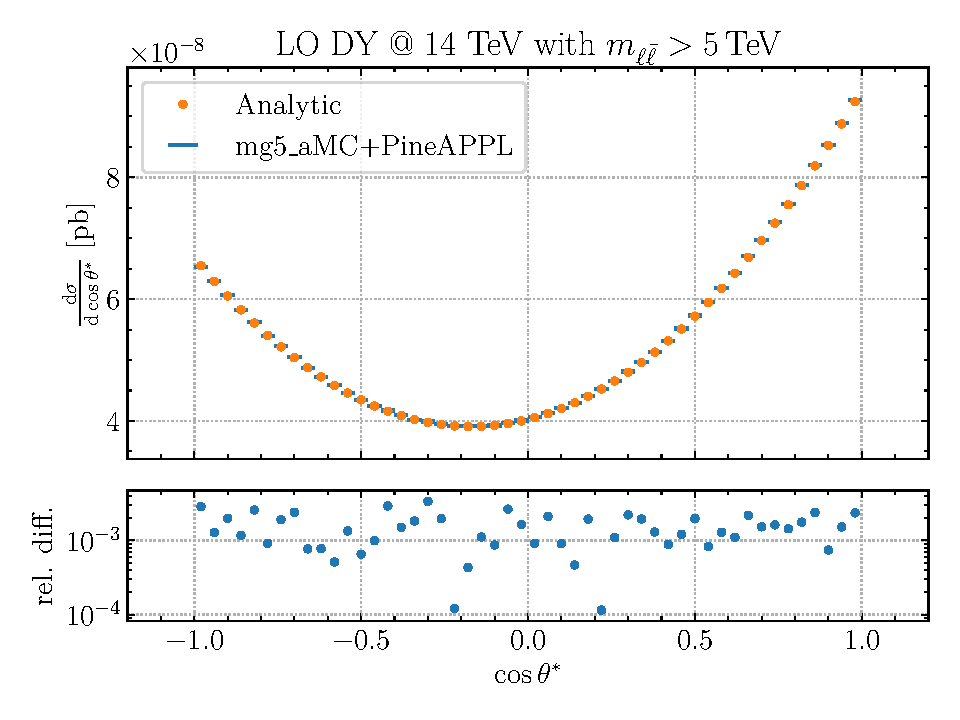
\includegraphics[width=0.49\linewidth]{ch-afb/sigma_grid_ana-MLL_5000_COSTH-r3.pdf}
  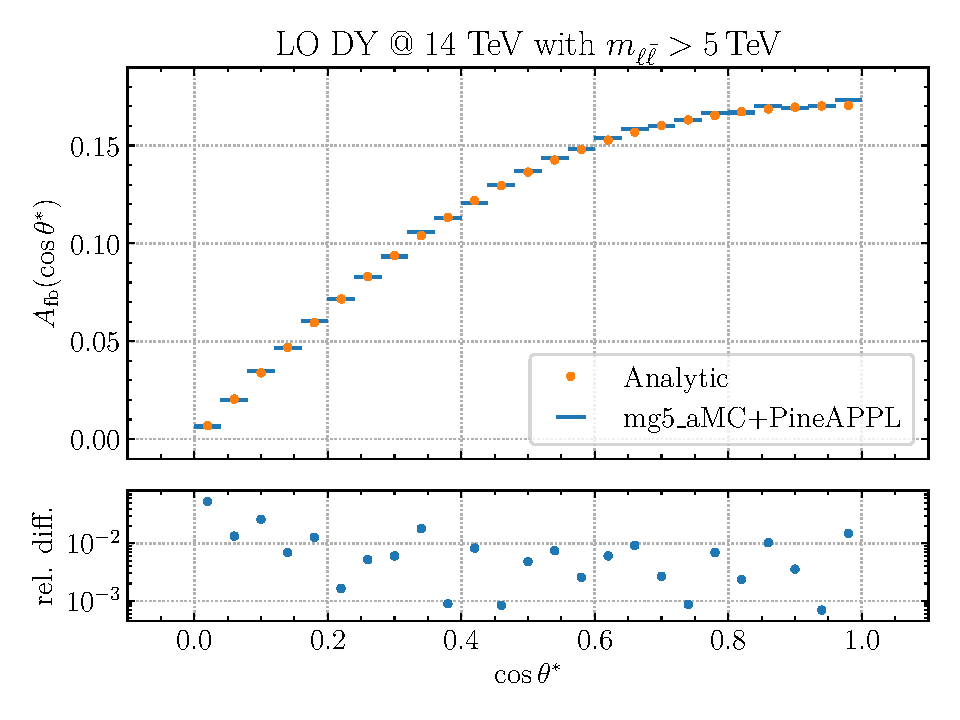
\includegraphics[width=0.49\linewidth]{ch-afb/afb_grid_ana-MLL_5000_COSTH-r3.pdf}
  \caption{The single-inclusive differential distribution in
    the Collins-Soper angle $\cos\theta^*$,
    \cref{eq:dsigma-dcos},
    and the corresponding forward-backward asymmetry computed at \lo,
    where the analytic calculation  \cref{eq:forward-backward-asymmetry}
    is compared with the numerical simulation based on 
    \mgamc
    interfaced to \pineappl.
    %
    The bottom panels display the relative difference between the analytic and
    numerical calculations.
    %
    One of the replicas of the \nnpdfr{4.0} \nnlo \pdf set is used as input
    to the calculation.
  }    
  \label{fig:lo-diff-cos}
\end{figure}
%%%%%%%%%%%%%%%%%%%%%%%%%%%%%%%

In order to illustrate concretely these results,  
in \cref{fig:lo-diff-cos} we display the
single-inclusive differential distribution in $\cos\theta^*$,
\cref{eq:dsigma-dcos},
and the corresponding forward-backward asymmetry,
\cref{eq:forward-backward-asymmetry} evaluated at \lo
for $\mll^{\text{min}}=\SI{5}{\TeV}$. The single-differential rapidity
distribution \cref{eq:dsigma-dyll}) is also shown for reference in Fig.~\ref{fig:lo-diff-yll}.
%
We display both a numerical evaluation based on \mgamc interfaced to \pineappl,
as well as analytic results found using the form \cref{eq:lo-triple-diff-lumis}
of the triple differential luminosity, with all the values of the parameters
entering \crefrange{eq:coup}{eq:propzz} set to the values used in the \mgamc
runcard, and performing  numerically the integrals in
\cref{eq:dsigma-dcos,eq:dsigma-dyll}.
%
For validation purposes, no kinematic cuts are applied to the rapidities and
transverse momenta of final-state leptons.
The \pdf input is taken to be given, for illustrative purposes, by one of the
replicas of the \nnpdfr{4.0} \nnlo set.
The relative difference between the analytic and numerical calculation is shown
in the bottom panels of \cref{fig:lo-diff-cos} and demonstrates perfect
agreement. 

While the discussion so far has been presented  at \lo, its qualitative
features are unaffected by  higher-order corrections.
%
To illustrate this, in \cref{fig:lo-kfact} we compare the \lo result  from
\cref{fig:lo-diff-cos} to the corresponding \nlo \qcd result.
%
The bottom panels display the \nlo $K$-factor for the $\cos\theta^*$
distribution and the forward-backward asymmetry.
%
Whereas the \nlo $K$-factor in the $\cos\theta^*$ distribution is quite large
(around 40\%) it exhibits only a mild dependence on the Collins-Soper angle.
%
For $A_{\text{fb}}$, the $K$-factor is at the 10\% level and essentially
independent of the value of $\cos\theta^*$.

%%%%%%%%%%%%%%%%%%%%%%%%%%%%%%%%%%%%
\begin{figure}[t]
  \centering
  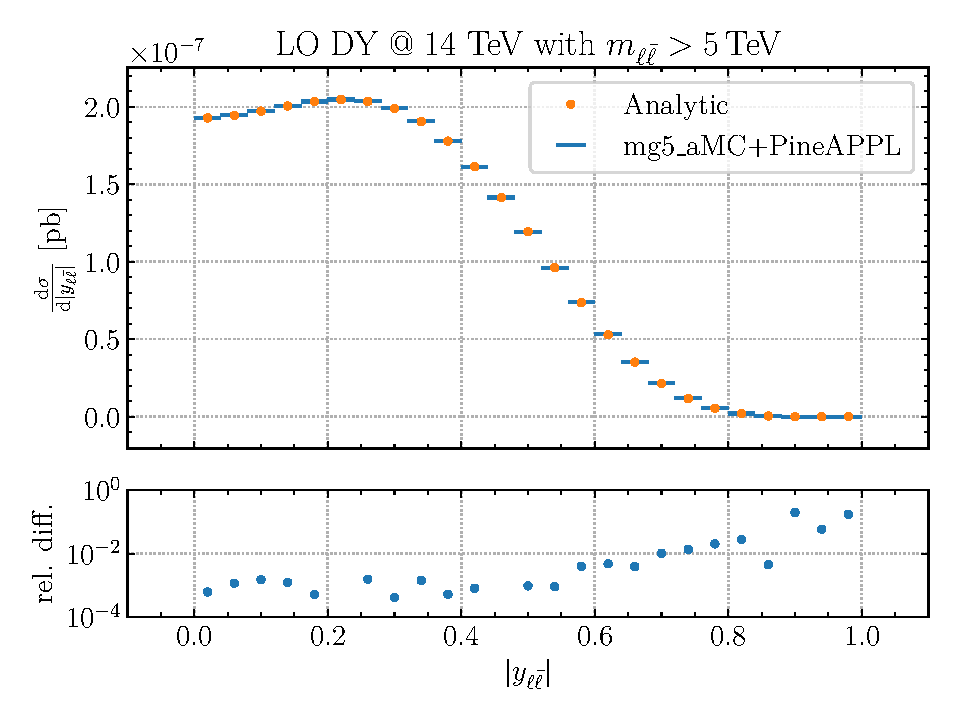
\includegraphics[width=0.49\linewidth]{ch-afb/sigma_grid_ana-MLL_5000_YLL-r3.pdf}
  \caption{Same as \cref{fig:lo-diff-cos} but now for the absolute dilepton rapidity distribution $|\yll|$}
  \label{fig:lo-diff-yll}
\end{figure}
%%%%%%%%%%%%%%%%%%%%%%%%%%%%%%%%%%%%%%%%%%
 
%%%%%%%%%%%%%%%%%%%%%%%%%%
\begin{figure}[t]
  \centering
  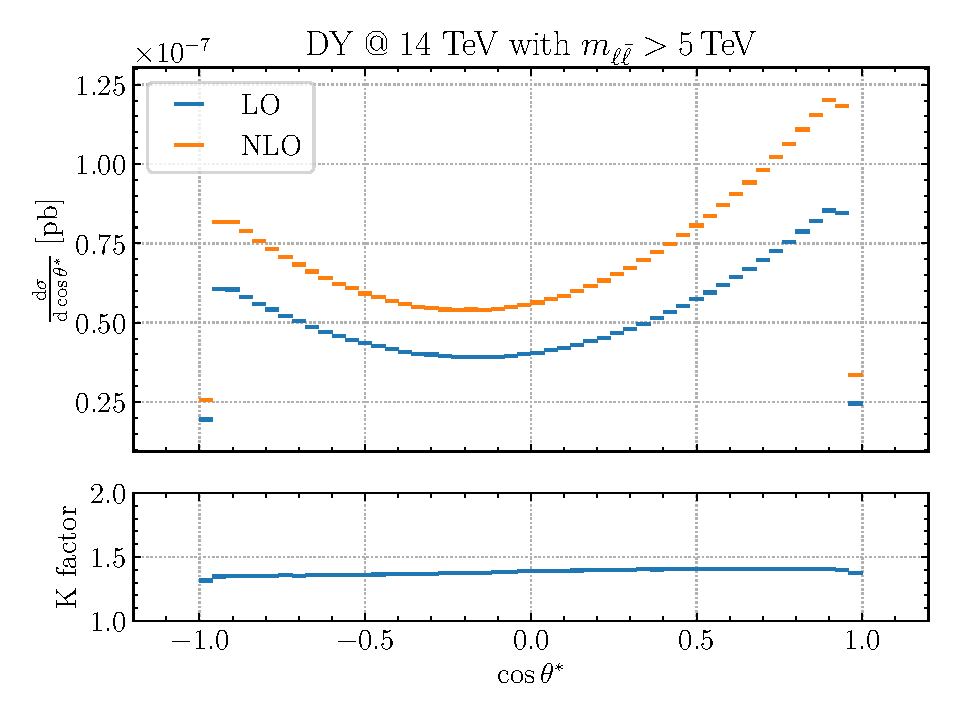
\includegraphics[width=0.49\linewidth]{ch-afb/sigma_lo_nlo-MLL_5000_COSTH-r3.pdf}
  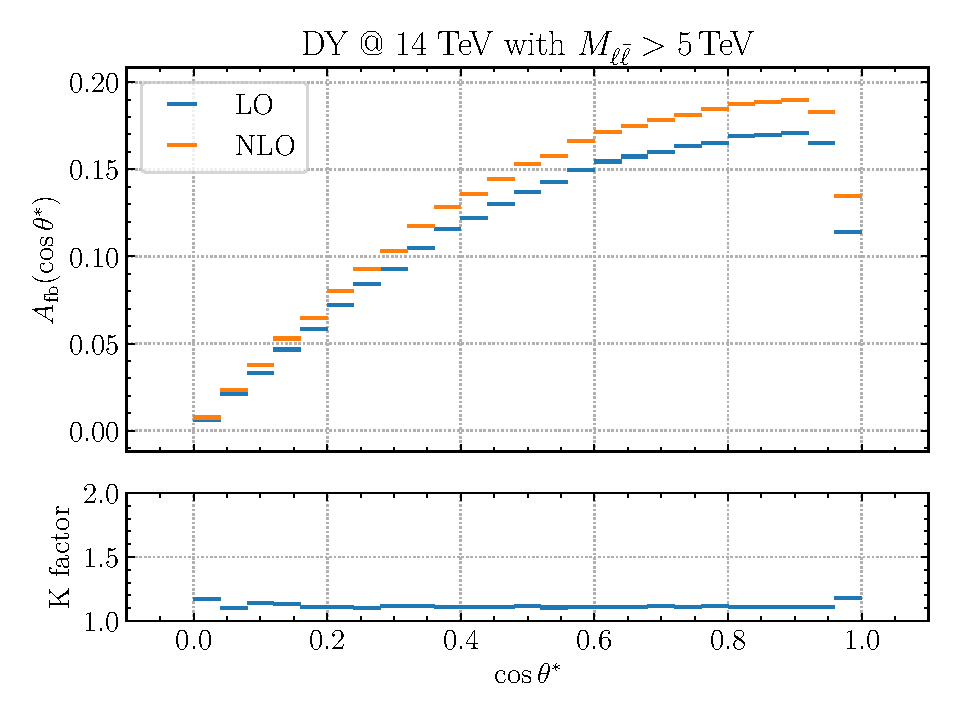
\includegraphics[width=0.49\linewidth]{ch-afb/afb_lo_nlo-MLL_5000_COSTH-r3.pdf}
  \caption{Same as \cref{fig:lo-diff-cos} now comparing the \lo result
    to the \nlo \qcd result obtained using \mgamc.
    %
    The $K$-factor is shown in the lower panel.
  }
  \label{fig:lo-kfact}
\end{figure}
%%%%%%%%%%%%%%%%%%%%%%%%%


\section{The forward-backward asymmetry and the large-\texorpdfstring{$x$}{x} \pdfs}
\label{sec:afb/largexpdfs}
% % !TeX root = ../../../main.tex

After our general discussion of the Drell-Yan process,
we now investigate
 proton structure at large-$x$, focusing on its
impact on the forward-backward asymmetry $A_{\rm fb}\lp \cos\theta^*\rp$
at large invariant masses.
%
First, we discuss the dependence of the
qualitative features of the asymmetry,
and specifically its sign, on the behavior of the underlying \pdfs: we
illustrate this in a toy model, and compare results to a simple and 
commonly used approximation.
%
Subsequently,
we study the large-$x$ behavior of the \pdfs from several
recent \pdf sets: we compare \pdfs, luminosities and the \lo asymmetry
$A_{\rm fb}$ as a function of the dilepton invariant mass $\mll$.

\subsection{Qualitative features of \texorpdfstring{$A_{\rm fb}$}{Afb}}
\label{sec:afb_toy}

In order to understand the main qualitative features of  the $\cos\theta^*$
distribution and of the asymmetry $A_{\rm fb}$ and their dependence on the 
properties of the underlying
\pdfs, it is instructive to evaluate predictions based on the
same computational setup adopted in Sect.~\ref{sec:HMDY}, namely
 \lo matrix elements without kinematic cuts, using toy \pdfs as input.
%
We consider toy quark and antiquark \pdf with  the form
\begin{equation}
  \label{eq:toypdf}
  xf_q(x) = A_qx^{-a_q}(1-x)^{b_q} \, , \quad xf_{\bar{q}}(x) = A_{\bar{q}}x^{-a_{\bar{q}}}(1-x)^{b_{\bar{q}}} \, ,
\end{equation}
where $A_q$ and $A_{\bar{q}}$ are  normalization constants, irrelevant
for this discussion.
%
For simplicity we neglect the scale dependence of
the \pdfs.
%
We then compute the single-differential distribution Eq.~(\ref{eq:dsigma-dcos}) and
the asymmetry Eq.~(\ref{eq:forward-backward-asymmetry}) with different assumptions on the
large $x$-behavior of these toy \pdfs, i.e.\ different values of the large-$x$
exponents $b_q$, $b_{\bar{q}}$.

Since the overall normalization does not affect the shape
of the distribution, we set $A_q=A_{\bar{q}}=1$.
%
Furthermore, since we are not interested in the small-$x$ behavior,
we set $a_q=a_{\bar{q}}=1$. 
%
Hence, we consider simple scenarios in which 
\begin{align}\label{eq:toyp}
xf_q^+(x; b_q,b_{\bar{q}}) &= xf_q(x)+xf_{\bar{q}}(x) = x^{-1}\lc (1-x)^{b_q} +(1-x)^{b_{\bar{q}}}  \rc  \,, \\\label{eq:toym}
xf_q^-(x; b_q,b_{\bar{q}}) &= xf_q(x)-xf_{\bar{q}}(x) = x^{-1}\lc (1-x)^{b_q} -(1-x)^{b_{\bar{q}}}  \rc  \,, 
\end{align}
with different choices of the parameters  $b_q$ and $b_{\bar{q}}$.
Specifically, we consider a scenario with $b_q < b_{\bar{q}} $, in particular
$(b_q,b_{\bar{q}})=(3,5)$, which leads to a positive valence combination $xf_q^-$
for all values of $x$;  a  scenario with
$(b_q,b_{\bar{q}})=(3,3)$ so  $xf_q^-$ vanishes identically; and a third scenario
in which the quark \pdfs at large-$x$ fall off more rapidly than the antiquarks,
$(b_q,b_{\bar{q}})=(5,3)$, so the valence combination $xf_q^-$ becomes negative.

%-----------------------------------------------------------------
\begin{figure}[!t]
 \centering
 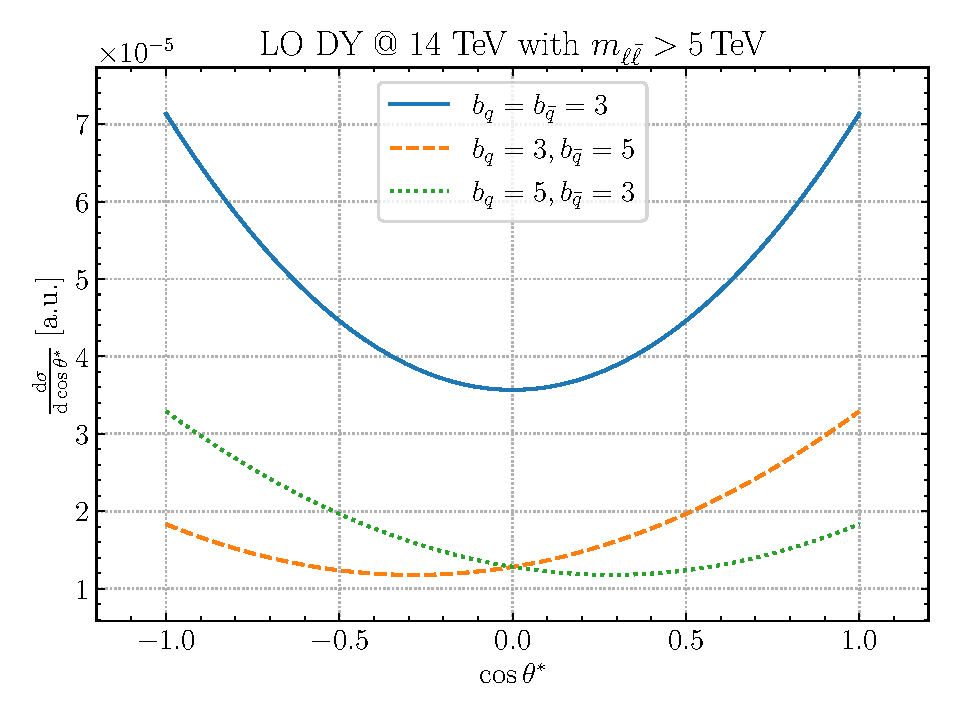
\includegraphics[width=0.49\linewidth]{ch-afb/sigma_toy-33-53-35.pdf}
 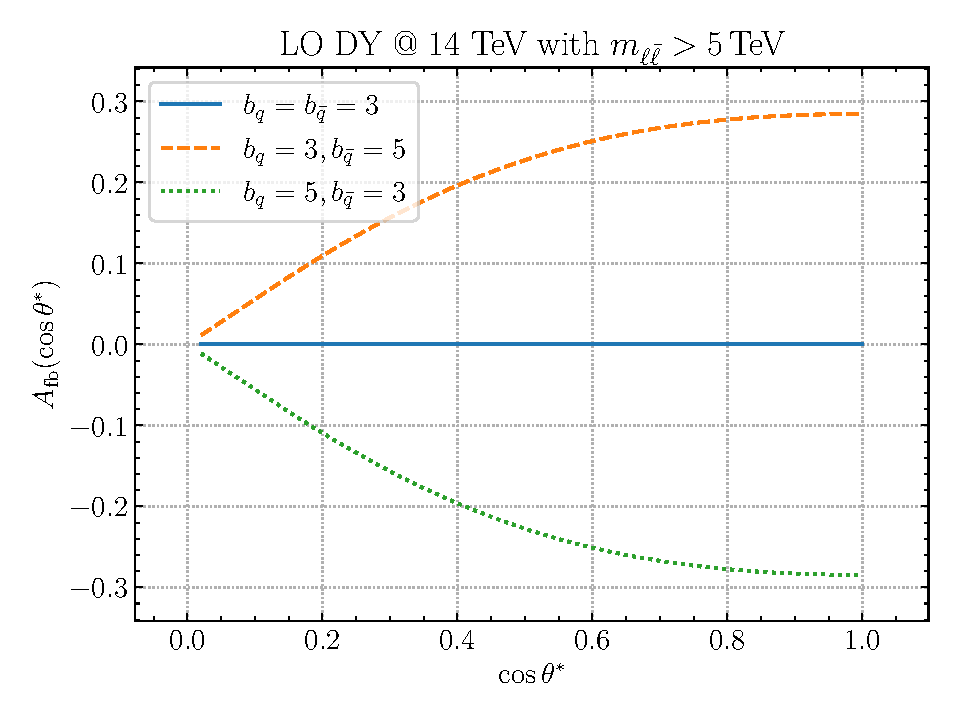
\includegraphics[width=0.49\linewidth]{ch-afb/afb_toy-33-53-35.pdf}
 \caption{The single-inclusive $\cos\theta^*$ distribution
   Eq.~(\ref{eq:dsigma-dcos})  (left)
   and the corresponding forward-backward asymmetry
   (right panel) Eq.~(\ref{eq:forward-backward-asymmetry}) evaluated using 
    the toy \pdfs of Eq.~(\ref{eq:toypdf}).
   %
   No  kinematic cuts are applied except for $\mll^{\rm min}=5$ TeV.
   %
 }    
 \label{fig:sigma_toy}
\end{figure}
%-----------------------------------------------------------------

In \cref{fig:sigma_toy} we display both the $\cos\theta^*$
single-inclusive distribution Eq.~(\ref{eq:dsigma-dcos}) and
the asymmetry Eq.~(\ref{eq:forward-backward-asymmetry}).
%
It is apparent that if the  antiquark \pdfs fall off at large-$x$ faster than
the quarks, i.e.\ when $b_q < b_{\bar{q}}$ the forward-backward
asymmetry is positive, while if the converse is true it is
negative. Of course if the quark and antiquark \pdfs behave in the same
way there is no asymmetry.
%
In this simple model, a negative asymmetry corresponds to a negative
valence distribution, which conflicts with sum rules and appears to be
unphysical. However, the model should be only taken as illustrative of
the large-$x$ behavior: it is of course easy to construct \pdfs that
reproduce this behavior at very large $x$, while leading to a positive
valence \pdf as $x$ decreases, consistent with sum rules. One could then argue that
Brodsky-Farrar counting rules~\cite{Brodsky:1973kr,Brodsky:1974vy}
imply that  $b_q > b_{\bar{q}}$
hence a positive asymmetry is favored.
%
However,
counting rules are supposed to only hold asymptotically, so whether
they apply in any given region of $x$ is a priori unclear.
%
It is easy
to construct generalizations of the model in which the behavior
leading to a negative asymmetry is reproduced at large enough $x$, yet
the valence \pdfs are positive at smaller $x$, and the counting rules
apply in the strict $x\to1$ limit.

In fact, whereas in the toy model a negative asymmetry is
associated with a negative valence
Eq.~(\ref{eq:toym}), the formal condition for a negative asymmetry is
(assuming $x_1>x_2$)
\begin{equation}\label{eq:signas}
   \sign\left[\mathcal{L}_{A,q}\right]=\sign\left[\frac{ f_q^+(x_2)}{
       f_q^+(x_1)}-\frac{
       f_q^-(x_2)}{f_q^-(x_1)}\right]=\sign\left[\frac{ f_q(x_2)}{
       f_q(x_1)}-\frac{f_{\bar{q}}(x_2)}{f_{\bar{q}}(x_1)}\right] \, , \quad x_1>x_2 \,.
\end{equation}
Hence what determines the sign of the antisymmetric luminosity, and thus
of the forward-backward asymmetry, is the relative rate of decrease of
the quark and antiquark, or valence and total quark \pdfs, rather than
their sign. Again, it is easy to construct generalizations of the
toy model in which the condition Eq.~(\ref{eq:signas}) still holds,  yet
the valence \pdf remains positive.

It is interesting to note that a different conclusion is reached using
an approximation to the asymmetry which is quite accurate  in the $Z$
peak region.
%
This approximation however turns out to fail at high
invariant mass.
%
Indeed, the expression Eq.~(\ref{eq:lumisa_qpm}) of the antisymmetric
luminosity in terms of the valence 
and total \pdf combinations $f_q^+$ and $f_q^-$ \pdf combinations
suggests an approximation based on the expectation
that the valence is dominant at large $x$ and the sea is dominant at
small $x$. Assuming $x_1> x_2$, one then expects that
\be
\mathcal{L}_{A,u}(\yll,\mll) \approx\frac {1}{2} f_u^-(x_1,\mll^2)
f_{u}^+(x_2,\mll^2)   \,  \, ,\quad x_1>x_2.
\label{eq:app_asym_lumi_2}
\ee
This is clearly true  in the $Z$-peak region, which  motivates the
suggestion to use the measurement of $A_{\rm fb}$ as a means to
 constrain the valence quark combinations~\cite{Accomando:2019vqt}.

%-------------------------------------------------------------------------------
\begin{figure}[!t]
 \centering
 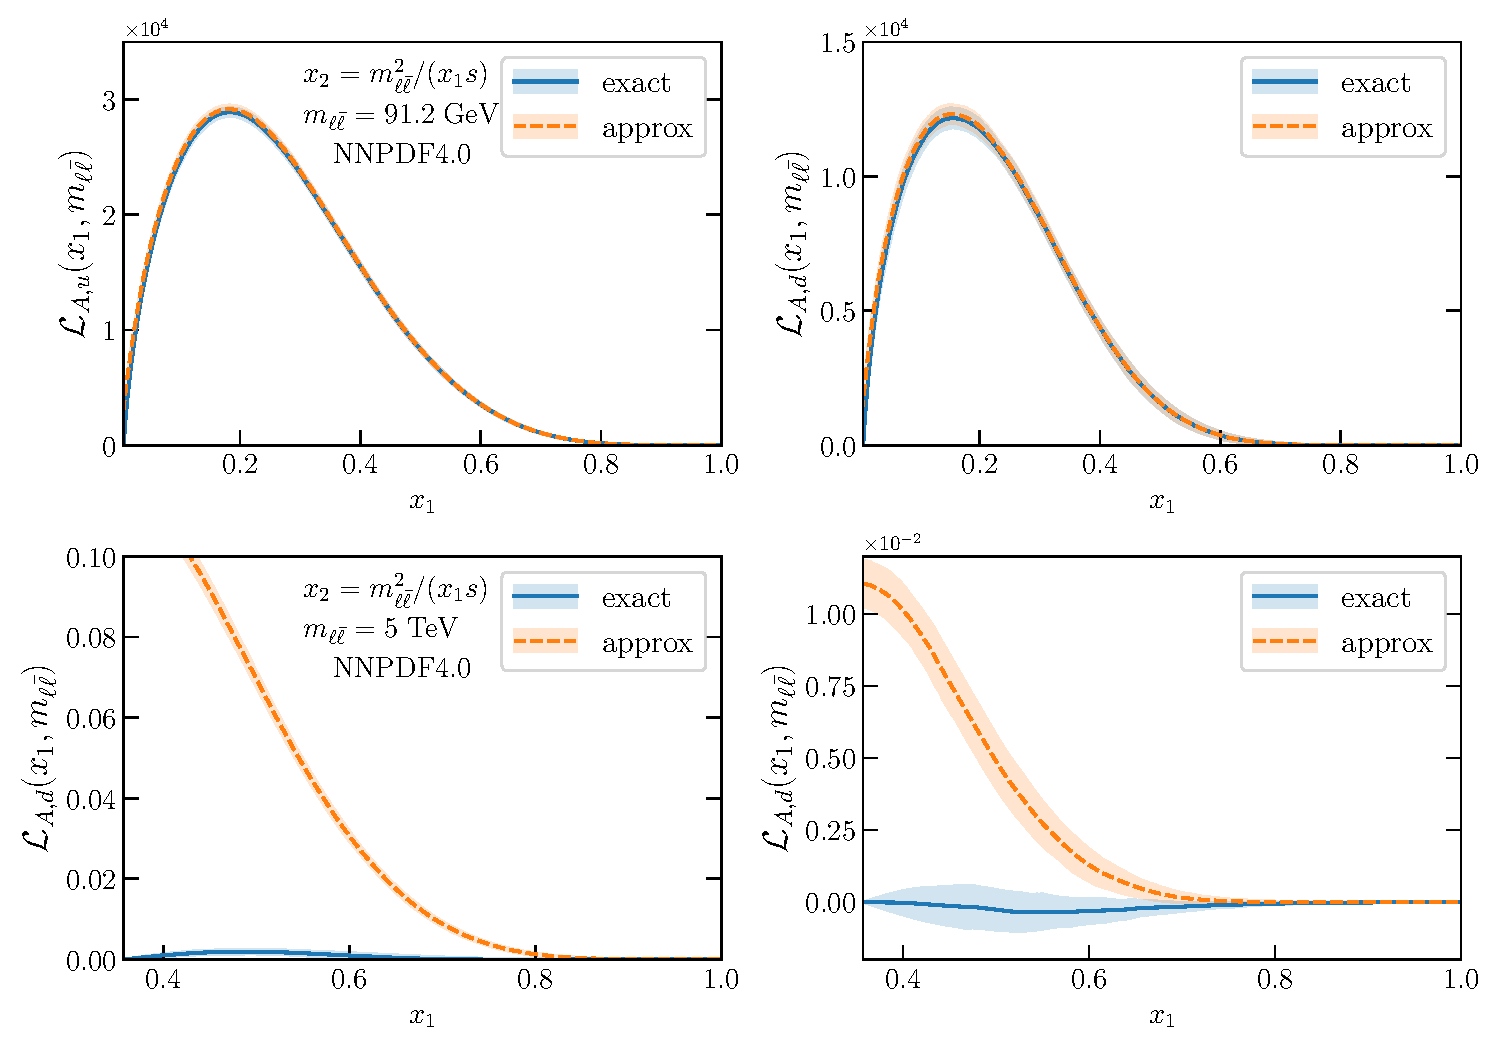
\includegraphics[width=0.90\linewidth]{ch-afb/pdfplot-abs-DYlumis-minus-validation-lowQ-nnpdf40.pdf}
 \caption{The  antisymmetric partonic luminosity $\mathcal{L}_{A,q}$, Eq.~(\ref{eq:lumisa_qpm}),
for the up and down quarks 
compared to the approximation 
Eq.~(\ref{eq:app_asym_lumi_2}) in the case of \nnpdfr{4.0}
at $\mll=m_Z$ (top)
and $\mll=5$ TeV (bottom panels).
 }    
 \label{fig:pdfplot-abs-DYlumis-minus-validation-lowQ-nnpdf40}
\end{figure}
%---------------------------------------------------------------------------

However, while Eq.~(\ref{eq:app_asym_lumi_2}) provides
a satisfactory approximation in the  $Z$-peak region,
it fails  at larger $\mll$ values. Indeed, for on-shell $Z$
production, with $\sqrt{s}=14$ TeV,
for a dilepton rapidity with $y_{\ell\bar{\ell}}\sim 2.5$, the limit of the
acceptance region
of ATLAS and CMS, the colliding partons have
$x_1=0.09$ and $x_2=6\times 10^{-4}$. So indeed the contribution in
which the valence \pdf is evaluated at the smallest $x$ value is highly suppressed.
%
But for $\mll=5$~TeV, the smallest value of $x_2$, attained when
$x_1=1$, is $x_2=0.35$: so both momentum fractions are large and in fact
to the right of the valence peak.
%
In such case, there 
is no obvious hierarchy between
the different terms that contribute to to antisymmetric
luminosity $\mathcal{L}_{A,q}$.

This is illustrated in
Fig.~\ref{fig:pdfplot-abs-DYlumis-minus-validation-lowQ-nnpdf40},
where we compare the antisymmetric luminosity $\mathcal{L}_{A,q}$
for the up and down quarks 
to the approximation
Eq.~(\ref{eq:app_asym_lumi_2}), evaluated with \nnpdfr{4.0} \nnlo,
in the $Z$-peak region $\mll=m_Z$ 
and at $\mll=5$ TeV.
%
While indeed for $\mll=m_Z$ Eq.~(\ref{eq:app_asym_lumi_2}) reproduces
the exact luminosity, this is not the case for $\mll\gg m_Z$: both
the magnitude and the shape of the luminosity are  very different.
%
This qualitative behavior is common to all \pdf sets: the approximation
fails equally badly regardless of the \pdf set.

We conclude that there
is no simple relation between the sign of the asymmetry and that of
the valence \pdf, and that the
behavior of the asymmetry must be determined by studying the large-$x$
behavior of the quark and antiquark \pdfs.

\subsection{Parton distributions}
\label{sec:subsec-largexPDFs}

We assess now the large-$x$ behavior of
the quark and antiquark \pdfs in different recent \pdf
determinations: specifically, we compare
 ABMP16,
 CT18,  \nnpdfr{4.0},
 and MSHT20.
%
 For
completeness, in App.~\ref{app:nnpdf31} we also present results
obtained with the widely used NNPDF3.1~\cite{Ball:2017nwa} set.

%-------------------------------------------------------------------------------
\begin{figure}[!t]
 \centering
 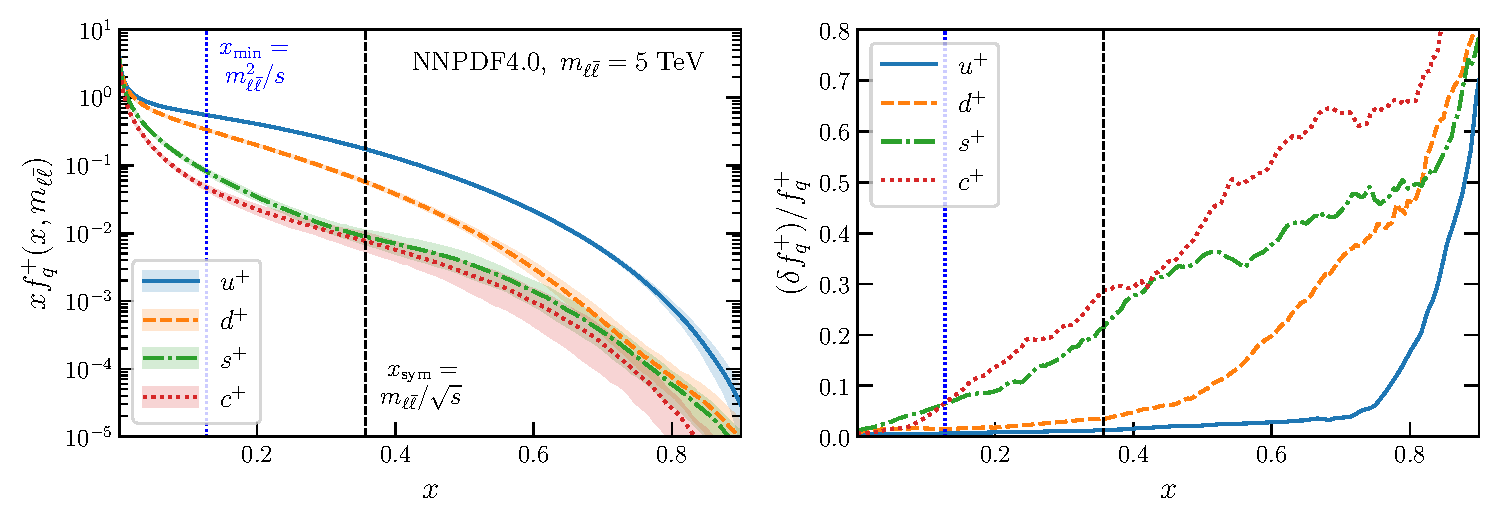
\includegraphics[width=1.0\linewidth]{ch-afb/pdfplot-abslargex-nnpdf40.pdf}
 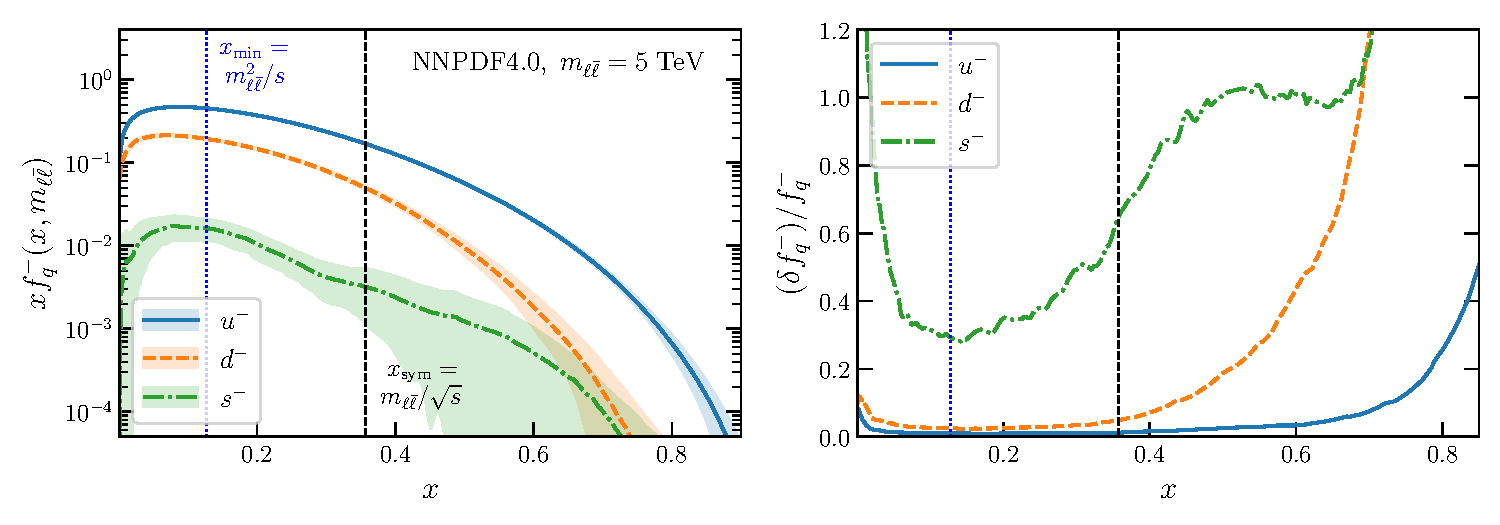
\includegraphics[width=1.0\linewidth]{ch-afb/pdfplot-abslargex-nnpdf40-valence.pdf}
 \caption{\small Comparison of the $xf^+_q$ (top) and $xf_q^-$ (bottom) quark
   \pdf combinations for the up, down, strange, and charm quarks,
   evaluated at $\mll=5$~TeV for \nnpdfr{4.0} \nnlo.
   %
   The right panels display the relative 68\% CL uncertainties.
   %
   The two vertical lines indicate $x_{\rm min}=\mll^2/s$, the
   smallest allowed value of $x$ 
   for dilepton DY production for a collider
   CoM energy $\sqrt{s}=14$~TeV, and the value of $x$
   corresponding to a symmetric partonic collision $x_1=x_2$, namely
 $x_{\rm  sym}=\mll/\sqrt{s}$.
 }    
 \label{fig:pdfplot-abslargex}
\end{figure}
%-------------------------------------------------------------------------------

First, we provide a qualitative assessment of the relative size of the
\pdfs corresponding to
individual quark flavors, both for the total and valence \pdfs.
In Fig.~\ref{fig:pdfplot-abslargex} we
compare  the total $xf^+_q$ and valence $xf_q^-$  quark
   \pdf combinations for the up, down, strange, and charm quarks,
   evaluated at $\mll=5$~TeV with the \nnpdfr{4.0} \nnlo \pdf set.
   %
   The right panels display the corresponding relative 68\% CL uncertainties.
   %
  The leftmost vertical line indicates $x_{\rm min}=\mll^2/s$, the
  smallest allowed value of $x$ 
   for dilepton DY production with invariant mass $\mll=5$~TeV for a collider
   CoM energy $\sqrt{s}=14$~TeV.
   %
   The rightmost vertical line corresponds to
   the value of $x$ in a symmetric partonic collision where $x_1=x_2$, namely
   $x_{\rm  sym}\equiv\mll/\sqrt{s}$.

   From Fig.~\ref{fig:pdfplot-abslargex} one can observe that for
   $x\lesssim 0.3$ there is a clear hierarchy
$f_u^+>f_d^+ >f_s^+>f_c^+$, while for larger $x$ values the
   strange and charm \pdfs become of comparable magnitude.
   %
   The up and down quarks, both for $xf^+_q$ and $xf^-_q$, are significantly larger
   than the second-generation quark \pdfs until $x\simeq 0.7$, and hence dominate the
   large-$\mll$ differential distributions in Drell-Yan production.
%
\pdf uncertainties grow rapidly with $x$, reflecting the lack
of direct experimental constraints.
%
The same qualitative behavior of the lighter versus heavier flavor \pdfs
is observed for other \pdf sets.
%
Given the hierarchy $f_u^\pm, f_d^\pm \gg f_s^\pm, f_c^\pm $, in the following
we will discuss only the behavior of the first-generation quark
and antiquark \pdfs which are those relevant for the interpretation
of neutral-current Drell-Yan production in the kinematic region used
for \bsm searches. 
      


%---------------------------------------------------------------------------
\begin{figure}[!t]
 \centering
 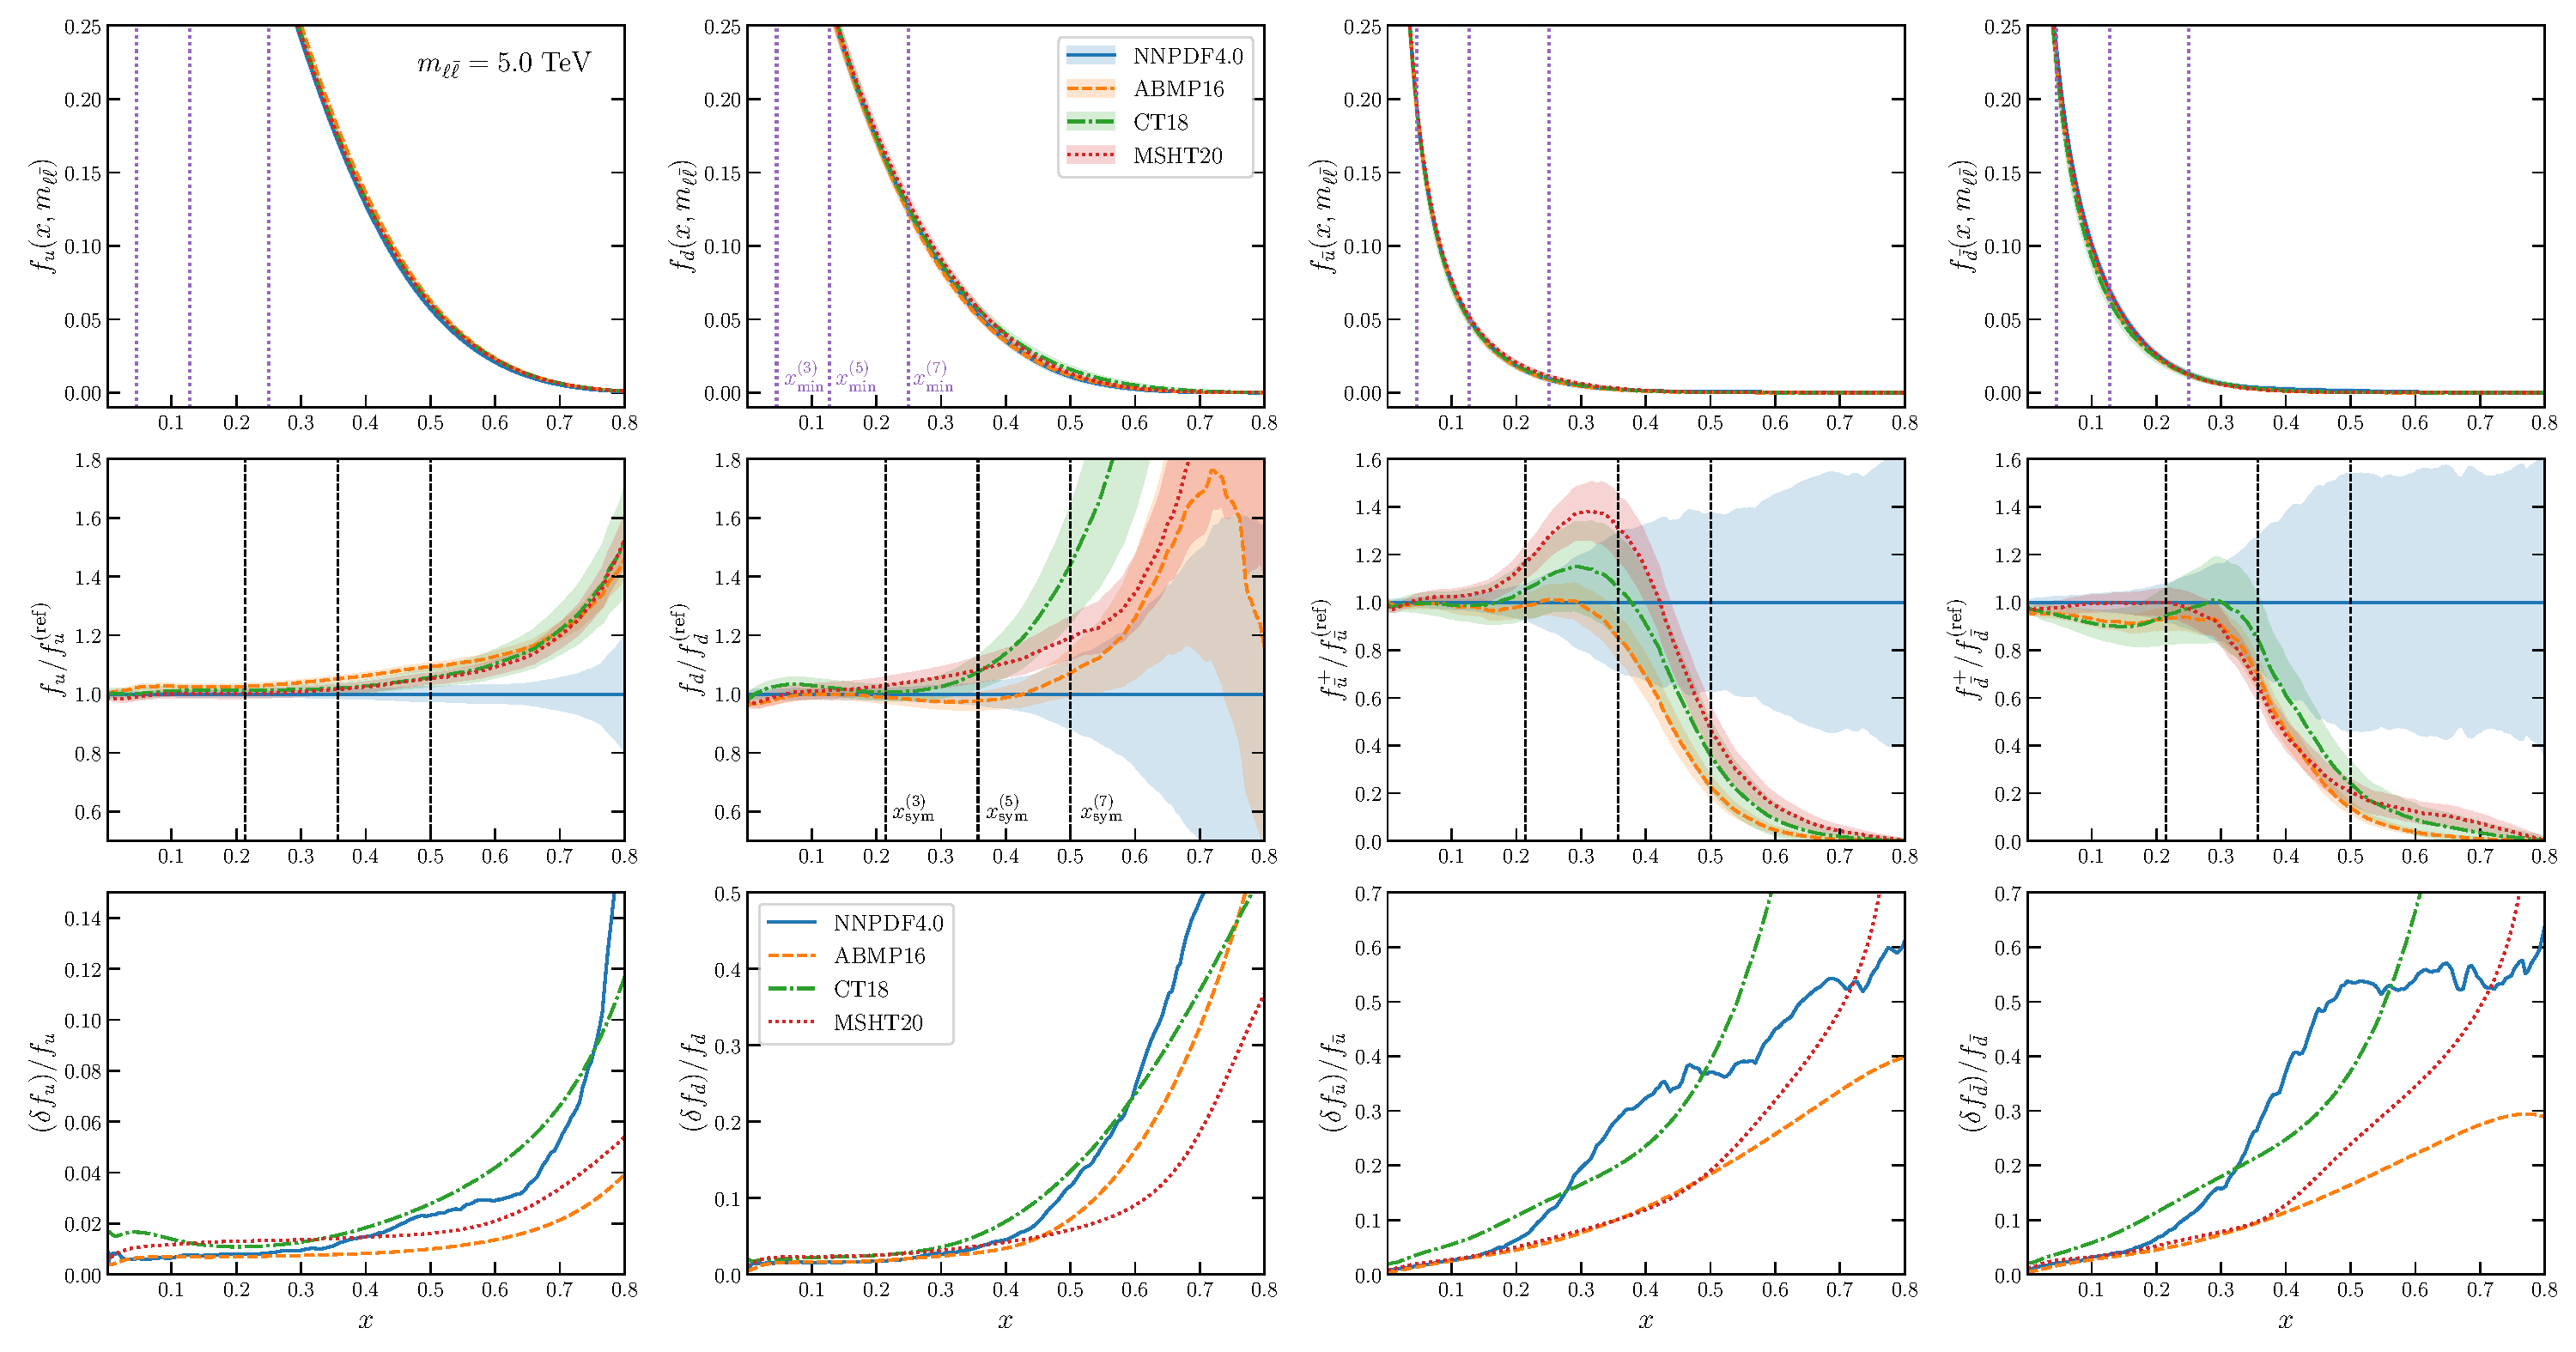
\includegraphics[width=1.00\linewidth]{ch-afb/pdfplot-pdfsets-quarks-antiquarks-q5p0tev.pdf}
 \caption{\small The up and down quark and antiquark \pdfs evaluated at $\mll=5$ TeV
   for \nnpdfr{4.0}, CT18, MSHT20, and ABMP16 in the $x$ region relevant for
   high-mass Drell-Yan production. The upper panels display the absolute \pdfs,
   the middle ones their ratio to the central \nnpdfr{4.0} value, and the bottom panels
   the relative 68\% CL uncertainties.
   %
   The vertical lines in the top
   row indicate the values of  $x_{\rm min}=\mll^2/s$ and in the central
   row those of $x_{\rm  sym}=\mll/\sqrt{s}$
   for three
   different values  $\mll=3,\,5,\,7$~TeV.
   %
   Note that in the second row the
   range on the $y$ axis is not the same for quarks and antiquarks,
   and in the third row also for up and down quarks.
   %
   Note also that the
   \pdfs, their ratios and their uncertainties are essentially
   unchanged in the displayed large-$x$ region in the range $1~{\rm TeV}<\mll<7$~TeV.
}    
 \label{fig:mll_dep_pdfs}
\end{figure}
%---------------------------------------------------------------------------

We next compare the large-$x$ behavior 
of the four \pdf sets ABMP16, CT18, MSHT20, and \nnpdfr{4.0} in Fig.~\ref{fig:mll_dep_pdfs}
for $\mll=5$~TeV.
%
We display from top to bottom the absolute \pdfs, their ratio to the central \nnpdfr{4.0} value, and
their relative 68\% CL uncertainties.
%
As in the case of Fig.~\ref{fig:pdfplot-abslargex}, we indicate with two vertical lines
the values of $x_{\rm min}$ and $x_{\rm  sym}$,
both for $\mll=5$~TeV, and for a smaller and a larger value of $\mll$,
namely for $\mll=3$~TeV and  $\mll=7$~TeV.
%
For clarity, the values of $x_{\rm min}$ are only shown 
in the top row of plots, and the values of  $x_{\rm  sym}$ in the
central row. Note that the scale dependence
of the \pdfs in this range of  $x$ and invariant mass is very
slight. Indeed, the \pdfs shown in Fig.~\ref{fig:pdfplot-abslargex} are
essentially unchanged at $\mll=3$ TeV or  $\mll=7$ TeV;  only the
corresponding ranges of $x_1$, $x_2$ vary significantly.

Good agreement between all \pdf
sets is found up to around $x\simeq 0.4$.
%
For $\mll=5$~TeV this corresponds to the value of $x_{\rm sym}$, i.e.\ central rapidity.
%
For larger values of $x\gsim 0.4$, the up  quark \pdf $xf_u$ from the
\nnpdfr{4.0} set is somewhat
suppressed in comparison to the other three sets, which in turn agree
among each other.
%
A rather stronger suppression of
\nnpdfr{4.0}  in comparison to  CT18 is observed for the down quark, with
MSHT20 and ABMP16 in a somewhat intermediate situation.
%
The opposite behavior is found in the same region $x\gsim 0.4$ for
antiquark \pdfs  $xf_{\bar{u}}$ and $xf_{\bar{d}}$:
namely, the \nnpdfr{4.0} \pdf is significantly  larger than that of the other sets.
It follows that for a lower invariant mass value  $\mll = 3$~TeV, all
\pdf sets are  in agreement in the $x$ range in which they are probed,
while for a higher value  $\mll = 7$~TeV the 
disagreement between \nnpdfr{4.0} and the other \pdf sets is present for
most of the $x\ge x_{\rm min}$ range.

It is interesting to observe that in the region with $0.4\lesssim x\lesssim
0.6$ the \pdfs are constrained by some fixed-target DIS structure functions and
by forward $W$ and $Z$ production data from \lhcb.
Hence, at the edge of the data region \nnpdfr{4.0} starts disagreeing with the
other global \pdf sets considered here, with the disagreement getting more
marked as $x$ grows outside the region covered by the data.
%
Qualitatively, \nnpdfr{4.0} is characterized by the fact that the
quark \pdfs drop faster as a function of $x$, and the antiquark \pdfs
drop less fast as $x$ grows towards $x=1$.
As we will show next, this feature will lead to significant differences
in the antisymmetric \pdf luminosities $\mathcal{L}_{A,q}$ as the value of
the dilepton invariant mass $\mll$ is increased.

The relative \pdfs uncertainties, shown in the lower panels in
Fig.~\ref{fig:mll_dep_pdfs} in all cases grow with $x$ (see also 
Fig.~\ref{fig:pdfplot-abslargex}).
%
The largest \pdf uncertainties correspond to either CT18 or \nnpdfr{4.0}, 
depending on the $x$ range and the \pdf flavor.
%
Specifically, the \nnpdfr{4.0} uncertainties are largest for $f_d$ in the
region $x\gsim 0.6$ 
and for $f_{\bar{u}}$ and $f_{\bar{d}}$ when $0.3 \lsim x \lsim 0.5$.
%
The smallest \pdf uncertainties are displayed by ABMP16 and  MSHT20.

The different behavior of the rate of decrease with $x$ of
\pdfs  in the large $x$ region, specifically comparing \nnpdfr{4.0}
to other \pdf sets, can  be seen most clearly from a comparison off
effective asymptotic exponents~\cite{Ball:2016spl}
\begin{equation}
  \beta_{a,q}(x,Q)\equiv\frac{\partial \ln|xf_q(x,Q)|}{\partial \ln(1-x)}\,,
  \label{eq:beta_asy}
\end{equation}
which of course for \pdfs of the form of Eq.~(\ref{eq:toypdf}) just
coincide with the exponent $b$ up to $O(1-x)$ corrections.
In Fig.~\ref{fig:asy_exponents} we compare
the values of $\beta_{a,q}(x,\mll)$
for ABMP16, CT18, MSHT20, and \nnpdfr{4.0} evaluated at $\mll=5$~TeV
for the up and down quark and antiquark \pdfs in the  $x$ range of
Fig.~\ref{fig:pdfplot-abslargex}.

It is clear that while all \pdf
sets have a similar effective asymptotic exponent for $x\lsim 0.35$, a
different behavior of \nnpdfr{4.0} in comparison to other
determinations sets in for $x\gsim 0.4$.
%
Specifically, for quarks the \nnpdfr{4.0} exponents are always larger,
and for antiquarks smaller than those found with other \pdf
sets.
%
Interestingly, whereas for the up quark the
effective exponent $\beta_{a,u}$ is approximately constant for all
\pdf sets when  $x\gsim 0.4$, with the \nnpdfr{4.0} value being just
slightly higher and slowly increasing, for the down quark and all
antiquarks this approximately constant behavior is seen for other
\pdf sets but not for \nnpdfr{4.0}.
%
Specifically, for the \nnpdfr{4.0} down quark
the exponent slowly but markedly increases for $x\gsim 0.3$, together 
with its uncertainty.
%
In the case of \nnpdfr{4.0} for both antiquarks the exponent
rapidly drops  in the region $0.3 \lsim x \lsim 0.4$.
%
This is consistent with the observation at the \pdf level
(Fig.~\ref{fig:mll_dep_pdfs})  that for \nnpdfr{4.0}
at large-$x$, as compared to the other groups,
the up and especially the down  quark fall off more rapidly, while
the antiquark \pdfs drop more slowly. Note in particular that for
the down \pdf the antiquark effective exponent is significantly
smaller than the quark effective exponent for all $x\gsim0.4$.

%-------------------------------------------------------------------------------
\begin{figure}[!t]
 \centering
 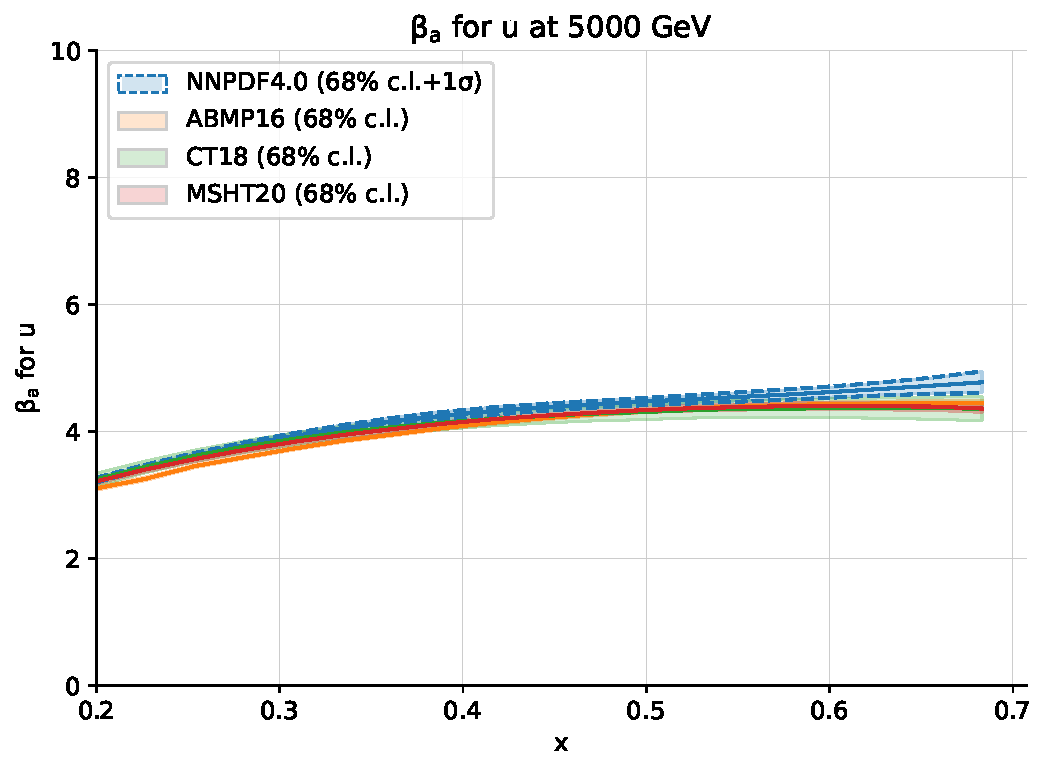
\includegraphics[width=0.49\linewidth]{ch-afb/beta_q_plot_beta_asy_u.pdf}
 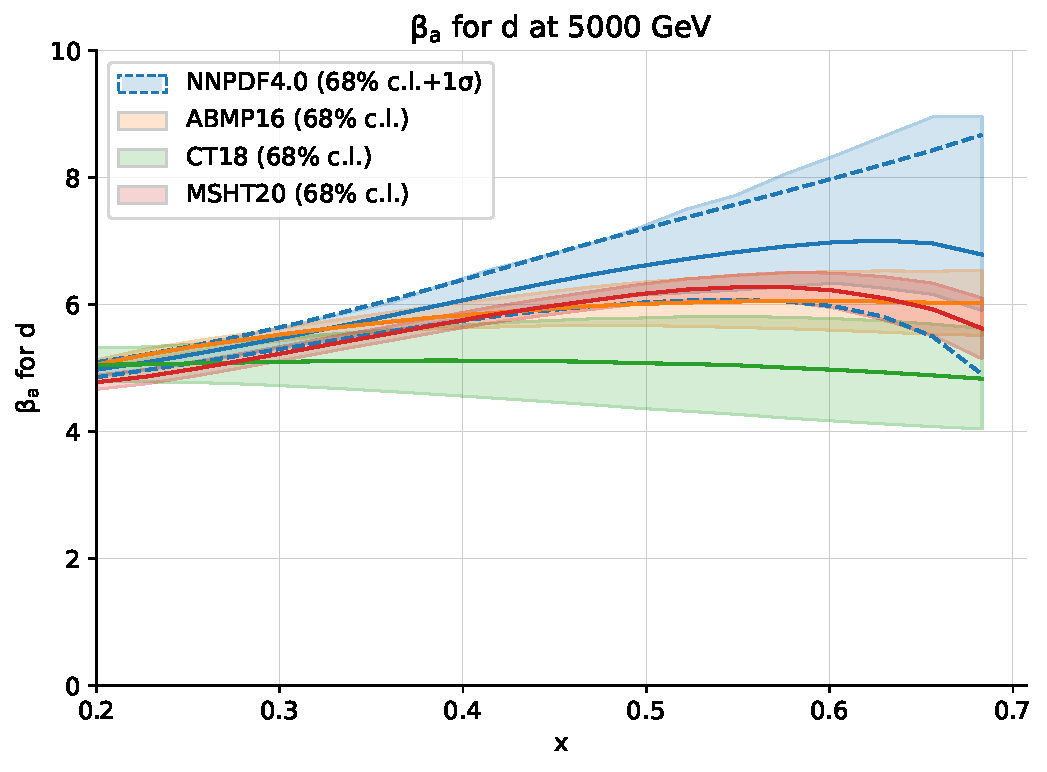
\includegraphics[width=0.49\linewidth]{ch-afb/beta_q_plot_beta_asy_d.pdf}
 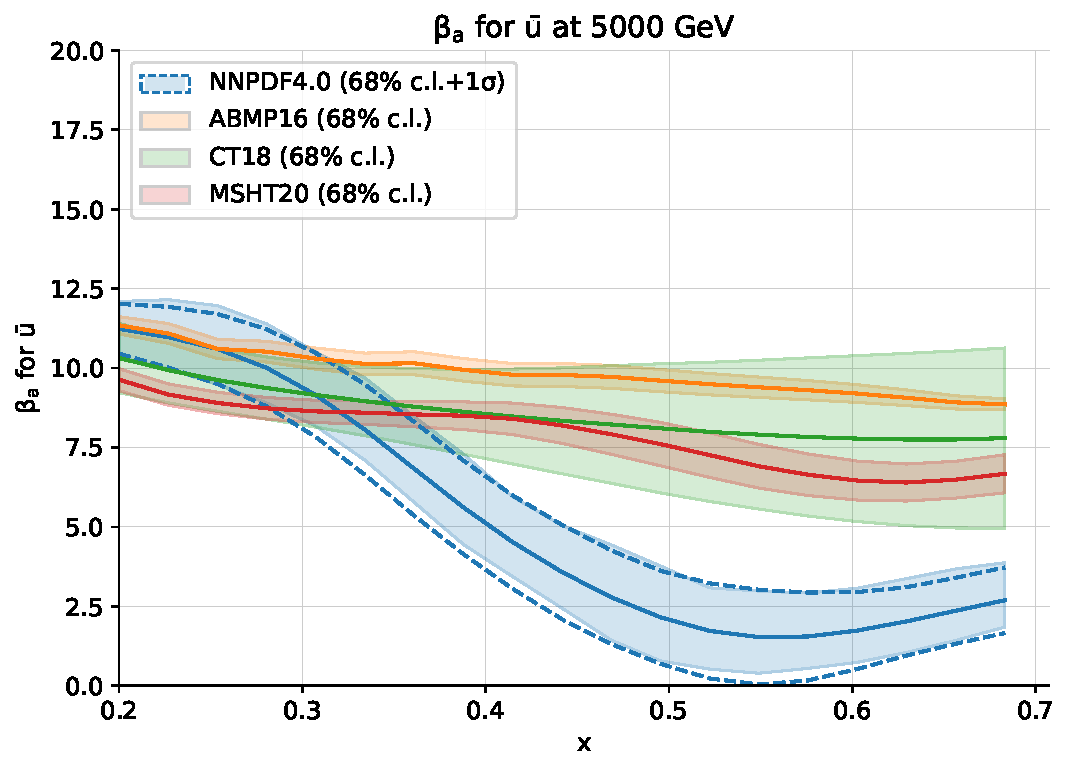
\includegraphics[width=0.49\linewidth]{ch-afb/beta_qbar_plot_beta_asy_baru.pdf}
 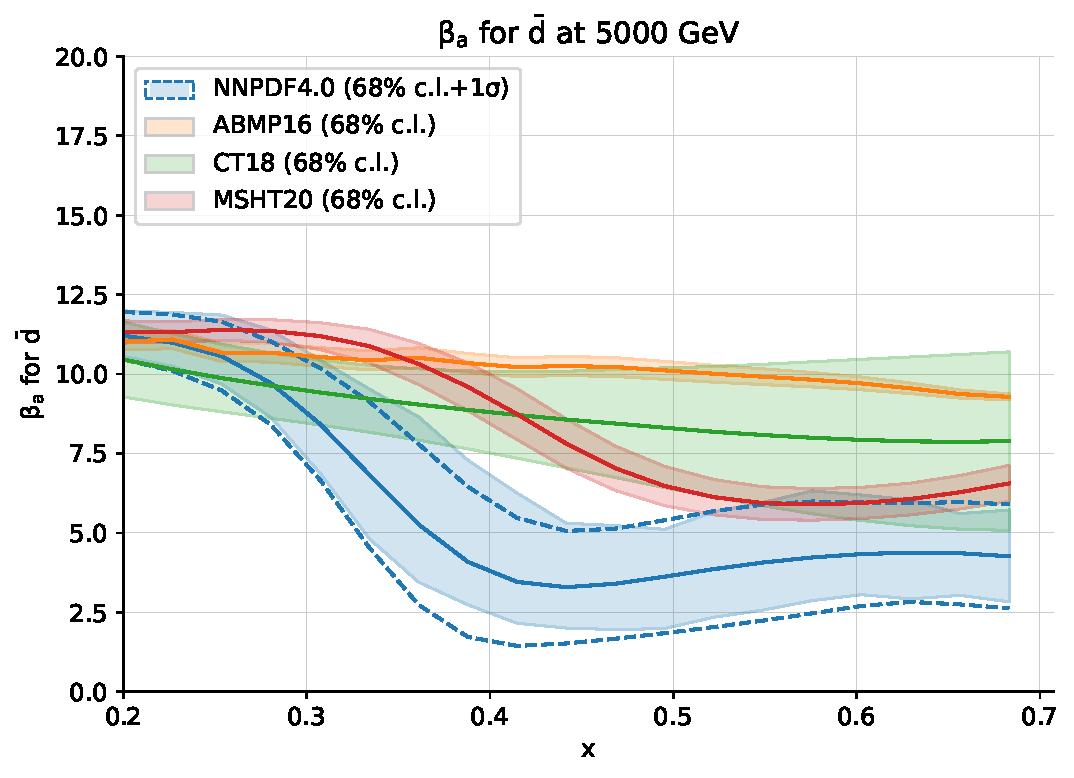
\includegraphics[width=0.49\linewidth]{ch-afb/beta_qbar_plot_beta_asy_bard.pdf}
 \caption{\small The large-$x$ asymptotic exponents $\beta_{a,q}(x,\mll)$, defined
   in Eq.~\eqref{eq:beta_asy},
   for ABMP16, CT18, MSHT20, and \nnpdfr{4.0} evaluated at $\mll=5$~TeV
   for the up and down quark and antiquark \pdfs.}    
 \label{fig:asy_exponents}
\end{figure}
%-------------------------------------------------------------------------------

The fact that a modification in behavior of the effective down quark
and especially antiquark \pdfs is observed at the edge of the data
region for \nnpdfr{4.0}, but not for other \pdf sets, suggests that this
might be related to the fact that  \nnpdfr{4.0} generally adopts a more
flexible \pdf parametrization in comparison to other groups.
%
Also, the  uncertainties on the effective exponents
$\beta_{a,q}(x,\mll)$ tend to be larger for \nnpdfr{4.0} (and also to a
lesser extent for CT18) in comparison to those of other groups.
Note however that the full \pdf uncertainty contains also a
contribution from the overall 
magnitude, which is not captured by the effective exponents displayed here.

\subsection{Parton luminosities}
\label{subsec:partoniclumis}

We finally turn to the behavior of parton luminosities, with
particular regard for the antisymmetric combination which is relevant
for the forward-backward asymmetry.
As for \pdfs, we first assess the qualitative features of the
luminosities corresponding to different quark flavors.
Specifically, the symmetric $\mathcal{L}_{S,q}$ and antisymmetric
$\mathcal{L}_{A,q}$ luminosities
Eq.~(\ref{eq:symm_asymm_lumis})  for individual flavors are
displayed in Fig.~\ref{fig:pdfplot-absDYlumis-plus-nnpdf40},
evaluated with \nnpdfr{4.0} \nnlo for $\mll=5$ TeV and $\sqrt{s}=14$ TeV.
%
The left panels display the absolute luminosities (in logarithmic and
linear scale respectively
for the $y$ and $x$ axes)
while the right panels show the corresponding \pdf uncertainties (relative and absolute for
$\mathcal{L}_{S,q}$ and $\mathcal{L}_{A,q}$, respectively).
%
The bottom  and top $x$-axes in each plot show respectively the values
of $x_1$ and $x_2$  at which the
luminosities are being evaluated, within the allowed range
$x \ge x_{\rm sym}=\mll/\sqrt{s}$, with the convention $x_1>x_2$.

%-------------------------------------------------------------------------------
\begin{figure}[!t]
 \centering
 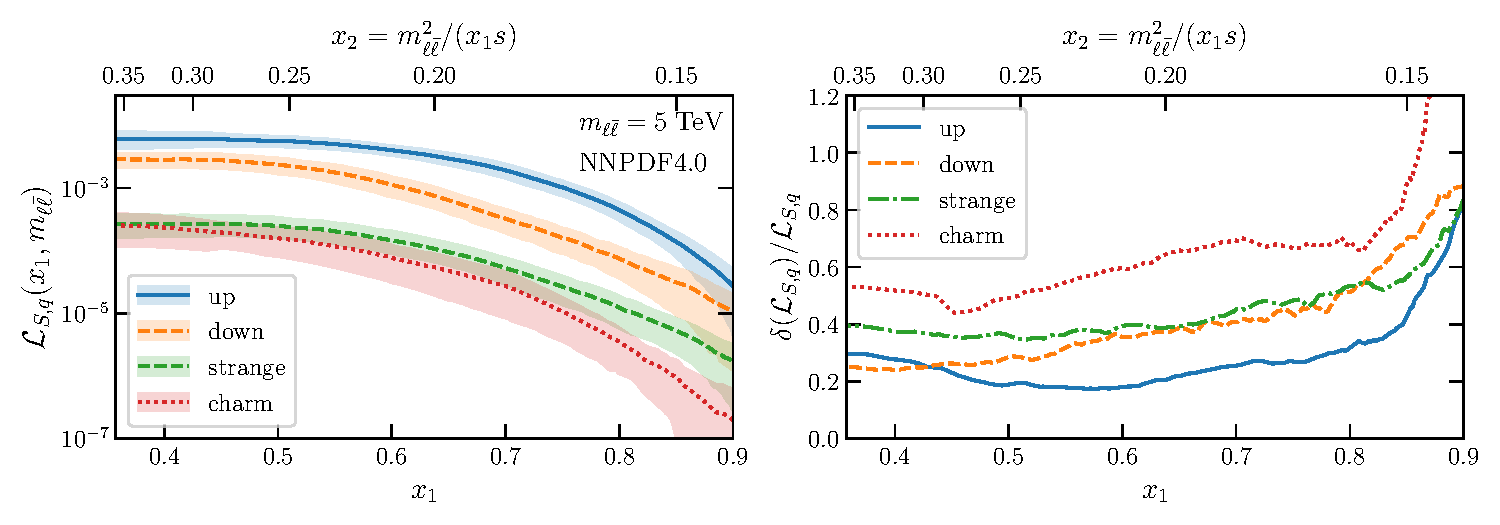
\includegraphics[width=\linewidth]{ch-afb/pdfplot-absDYlumis-plus-nnpdf40.pdf}
 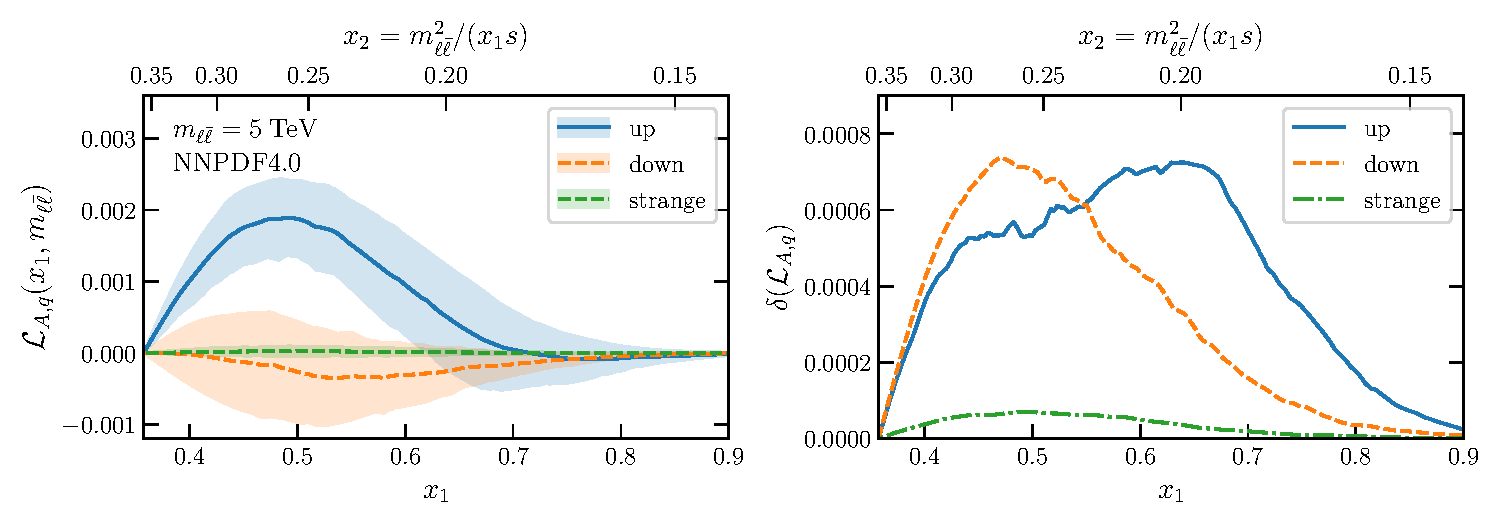
\includegraphics[width=\linewidth]{ch-afb/pdfplot-absDYlumis-minus-nnpdf40.pdf}
 \caption{The symmetric $\mathcal{L}_{S,q}$ (top)
   and antisymmetric $\mathcal{L}_{A,q}$ (bottom)
   parton
   luminosities (left) and relative uncertainties (right) evaluated with
   \nnpdfr{4.0} \nnlo at $\mll=5$ TeV and $\sqrt{s}=14$ TeV.
   %
The bottom  and top $x$-axes in each plot show respectively the values
of $x_1$ and $x_2$  at which the
luminosities are being evaluated, within the allowed range
$x \ge x_{\rm sym}=\mll/\sqrt{s}$, with the convention $x_1>x_2$.}    
 \label{fig:pdfplot-absDYlumis-plus-nnpdf40}
\end{figure}
%---------------------------------------------------------------------------

The symmetric parton luminosities exhibit of course the same hierarchy
between flavors
as the corresponding \pdf plots of Fig.~\ref{fig:pdfplot-abslargex}. 
%
The luminosity $\mathcal{L}_{S,q}$  drops rapidly for
$x_1\gsim 0.6$. \pdf  uncertainties  depend weakly on  $x$
up to $x_1\gsim 0.8$, after which they blow up, and range between $\sim 20\%$
for the up quark luminosity to $\sim 60\%$ for the charm quark one,
with down and strange intermediate and of similar magnitude.

As displayed in Fig.~\ref{fig:mll_dep_lumi_plus}, the light quark symmetric luminosities of other global \pdf sets
are qualitatively similar.
%
We show $\mathcal{L}_{S,u}$,  $\mathcal{L}_{S,d}$,
and their weighted sum that enters the  enters the
symmetric coefficient $g_{S,q}$ in Eq.~(\ref{eq:dsigma-dcos-v2})
for the \nnpdfr{4.0}, ABMP16,
CT18, and MSHT20 at $\mll=5$ TeV.
%
The luminosities are multiplied by the effective charges
$S_q$ defined in Eq.~(\ref{eq:coup}),
and the bottom panels display the corresponding 68\% CL \pdf uncertainties.
%
Good agreement between the four sets, with a similar shape
of $\mathcal{L}_{S,q}$, is observed.
%
The \pdf luminosities for the dominant $\mathcal{L}_{S,u}$ contribution are the largest for \nnpdfr{4.0}.

%-------------------------------------------------------------------------------
\begin{figure}[!t]
 \centering
 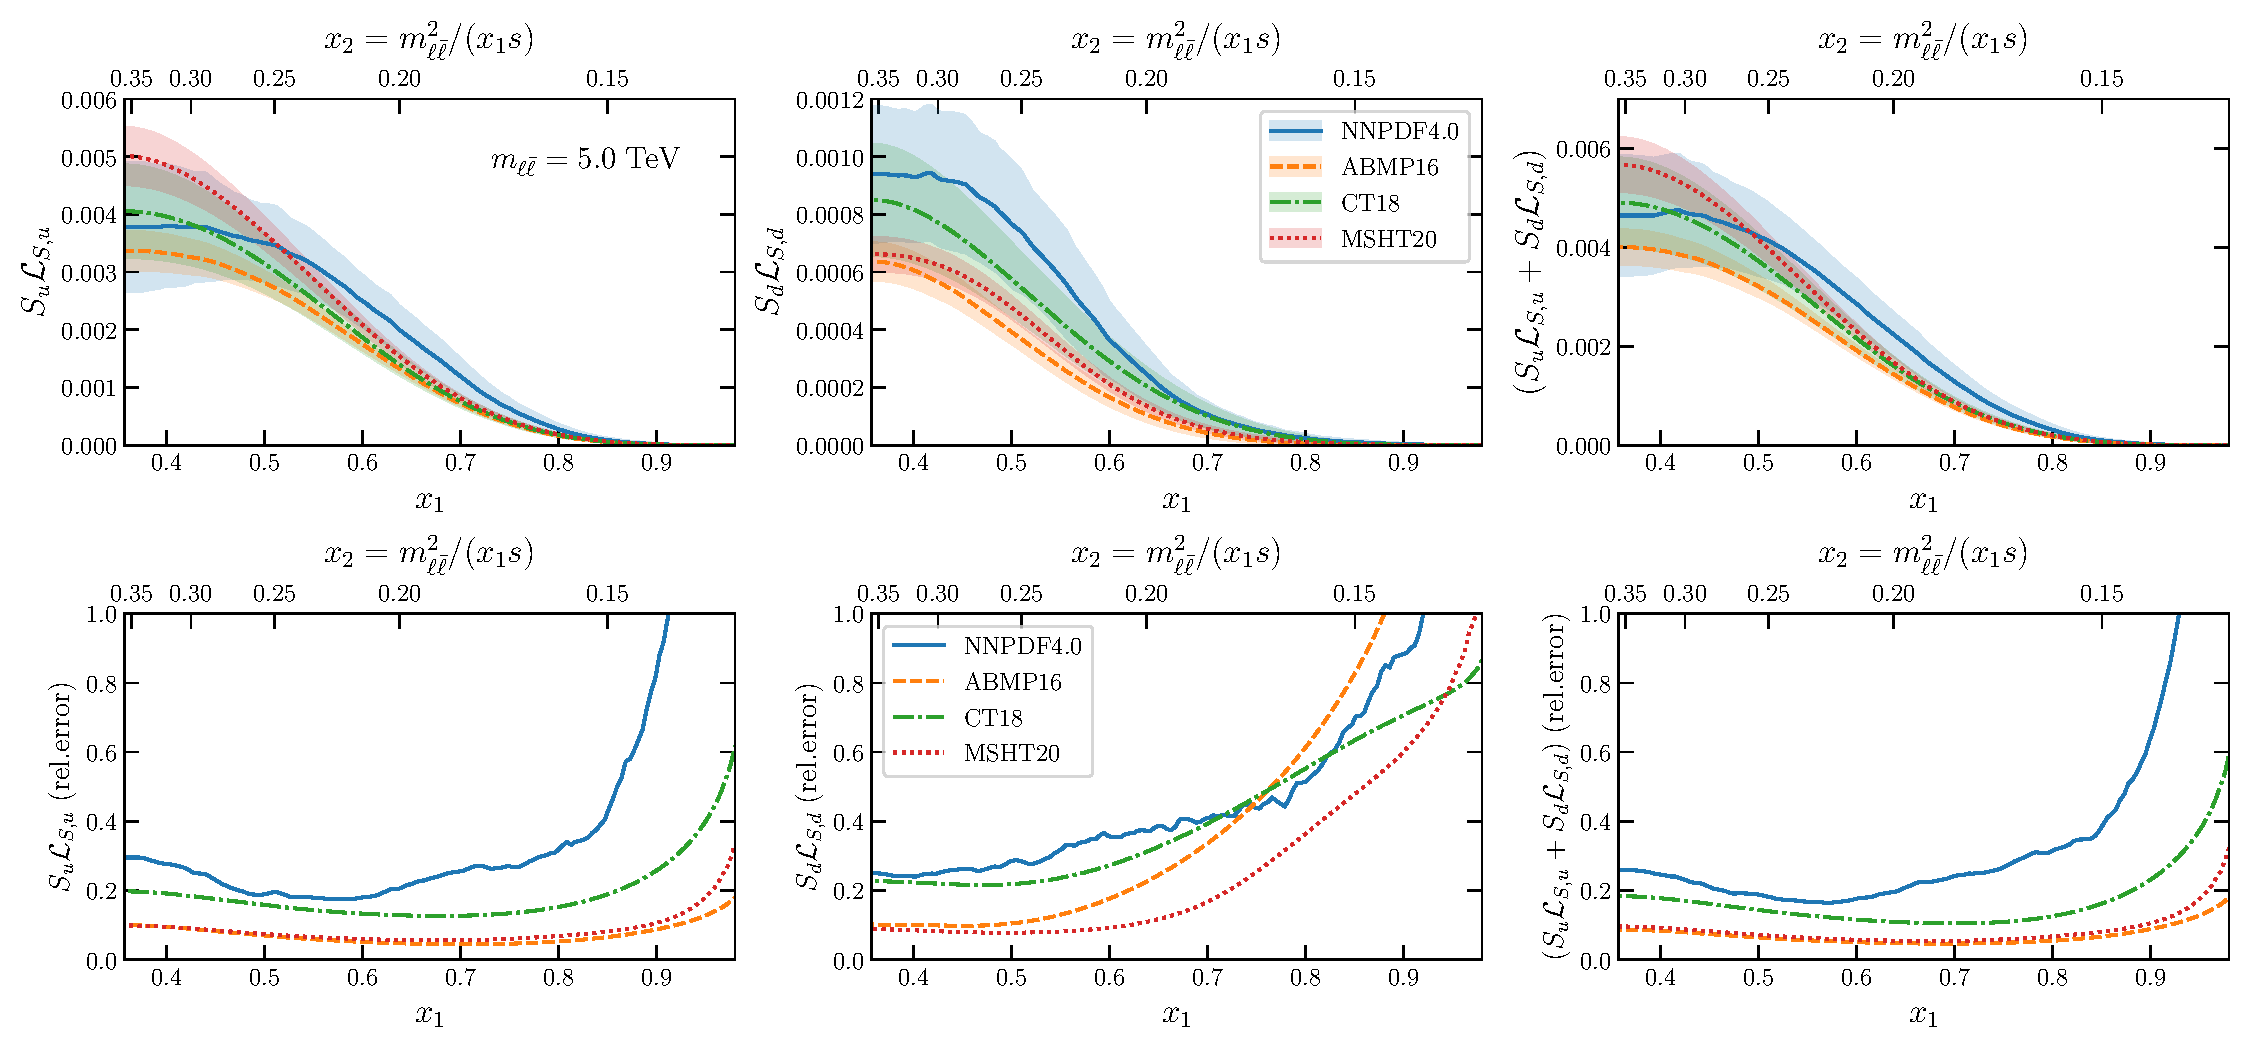
\includegraphics[width=1.00\linewidth]{ch-afb/pdfplot-abs-jacobian-DYlumis-pdfsets-plus-q5p0tev.pdf}
  \caption{The symmetric 
   parton luminosities $\mathcal{L}_{S,q}(x_1,\mll)$ for the \nnpdfr{4.0}, ABMP16,
   CT18, and MSHT20 \nnlo \pdf sets for dilepton
   invariant masses of $\mll=5$ TeV.
   %
   The luminosities are multiplied by the effective charges
   $S_q$ defined in Eq.~(\ref{eq:coup}).
   %
   From left to right, we display $\mathcal{L}_{S,u}$,  $\mathcal{L}_{S,d}$,
   and their weighted sum that enters the  coefficient $g_{S,q}$ in Eq.~(\ref{eq:dsigma-dcos-v2}).
   %
   The bottom panels display the relative 68\% CL \pdf uncertainties.
    }    
 \label{fig:mll_dep_lumi_plus}
\end{figure}
%---------------------------------------------------------------------------

Turning to the antisymmetric \pdf luminosities $\mathcal{L}_{A,q}$,
we note  that, for \nnpdfr{4.0}, while the up luminosity is
positive, the central value of the down luminosity is negative, though
the luminosity is compatible with zero at the one sigma level.
%
Recalling
from Fig.~\ref{fig:pdfplot-abslargex} that $xf_{d}^-$ itself is
positive for all values of $x$,  this provides an explicit example in
which the condition Eq.~(\ref{eq:signas}) is satisfied without the valence
combination being negative.
%
We conclude that for \nnpdfr{4.0}, the faster
drop of the quark distribution and slower drop of the antiquark
distribution that was displayed by the effective exponents of
Fig.~\ref{fig:asy_exponents} leads to a negative antisymmetric
luminosity, in agreement with Eq.~(\ref{eq:signas}).
The absolute \pdf uncertainties are of a similar size for
$\mathcal{L}_{A,u}$ and $\mathcal{L}_{A,d}$, with a different shape
reflecting the underlying central values.

We compare
in Fig.~\ref{fig:mll_dep_lumi_minus}
the behavior of the antisymmetric luminosities for all \pdf
sets for $\mll=3$ TeV (top) and $\mll=5$ TeV (bottom).
%
In order to facilitate the understanding of the way the \pdf behavior
determines that of the asymmetry, we show both the contribution of
individual flavors and the total contribution
to the antisymmetric coefficient $g_{A,q}$ of
Eq.~(\ref{eq:gAq_integrated_1}). Namely, in
Fig.~\ref{fig:mll_dep_lumi_minus} the luminosities corresponding to
individual flavors are multiplied by the corresponding flavor-dependent
effective charges $A_q$ defined in Eq.~(\ref{eq:coup}):
from left to right we display $\mathcal{L}_{A,u}$,  $\mathcal{L}_{A,d}$,
and their weighted sum
 which determines
the sign and magnitude of the total forward-backward asymmetry.
%
The corresponding absolute \pdf uncertainties for each of the four \pdf sets
are displayed in  Fig.~\ref{fig:mll_dep_lumi_minus_pdferrs}.

%-------------------------------------------------------------------------------
\begin{figure}[!t]
 \centering
 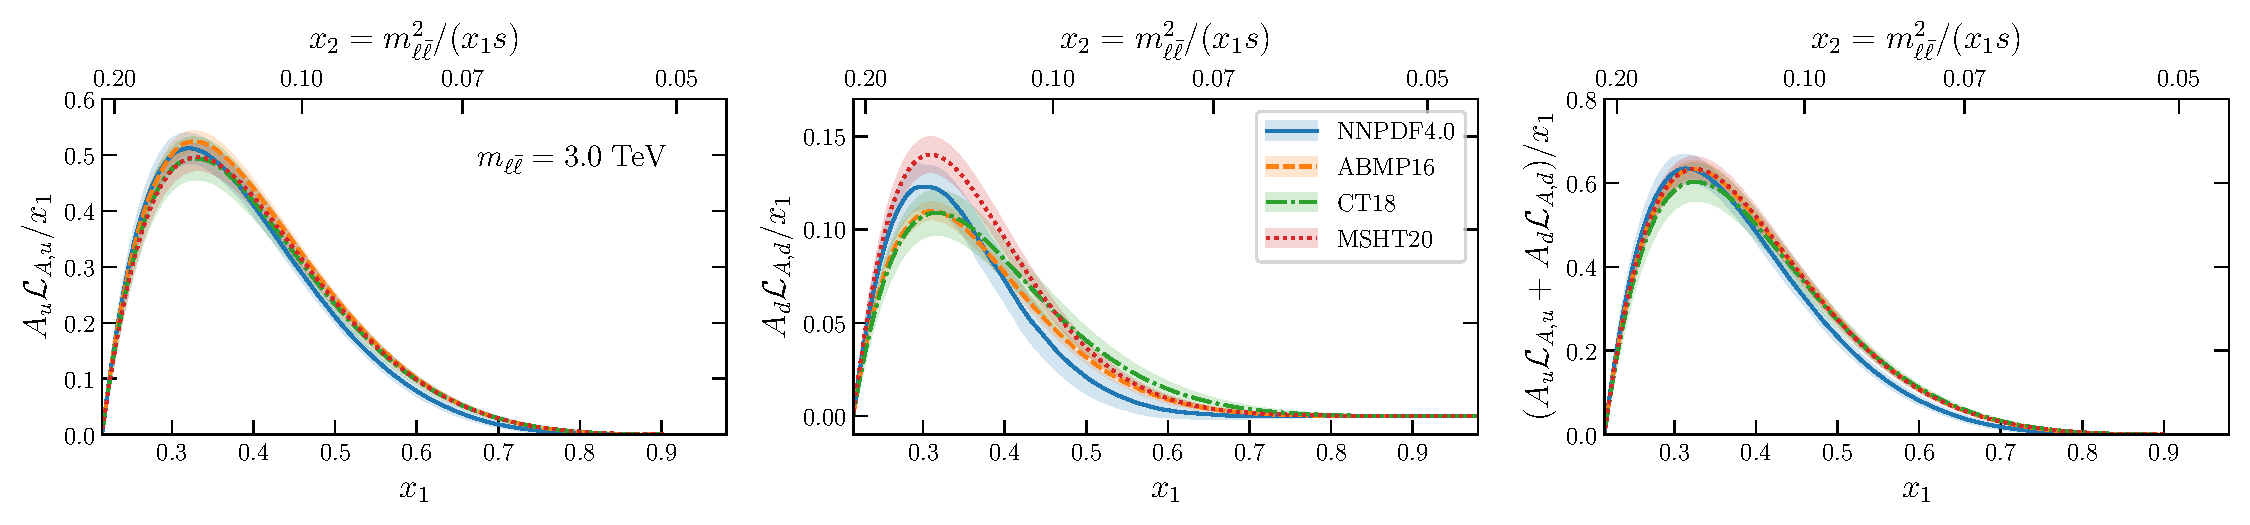
\includegraphics[width=1.00\linewidth]{ch-afb/pdfplot-abs-jacobian-DYlumis-pdfsets-minus-q3p0tev.pdf}
 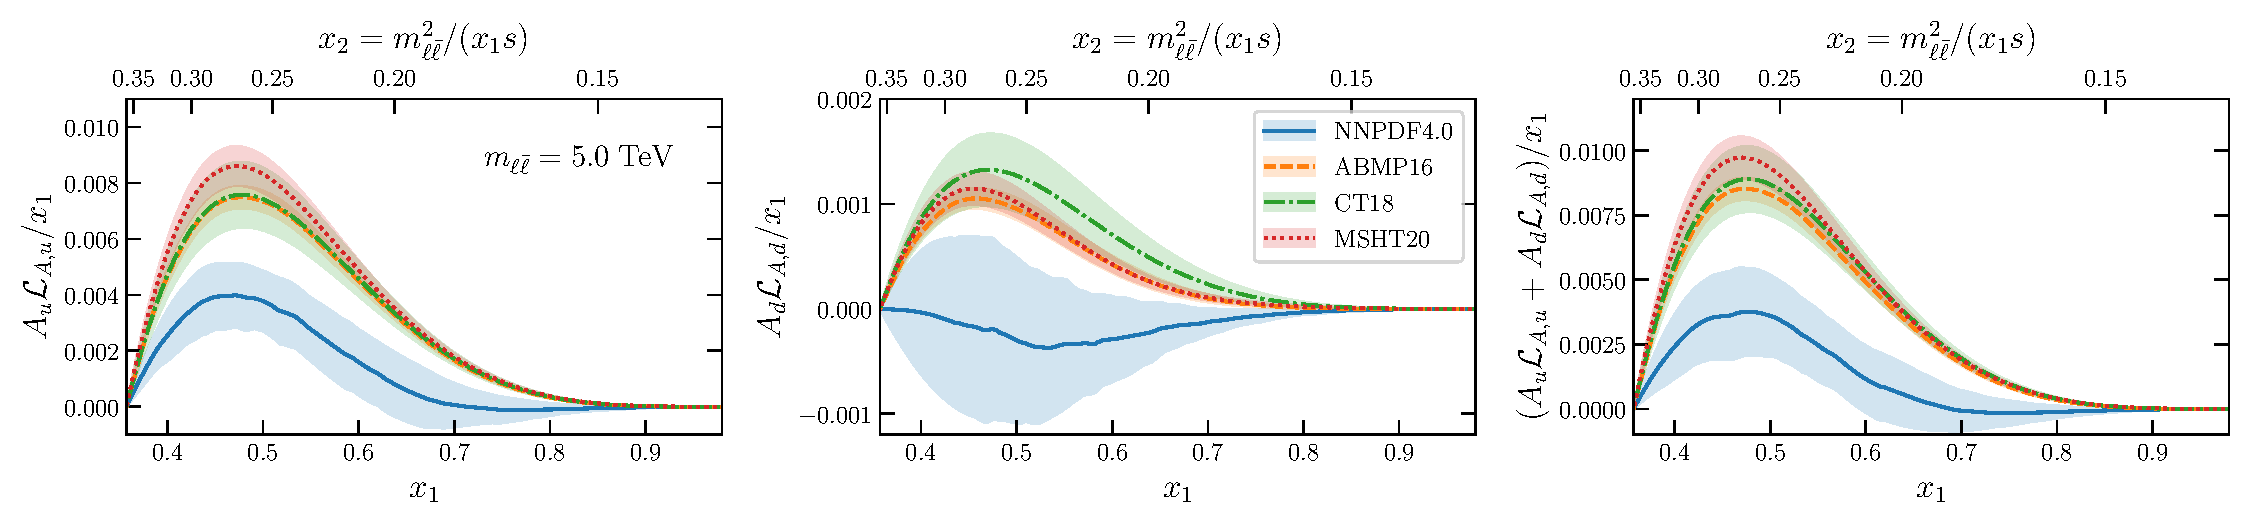
\includegraphics[width=1.00\linewidth]{ch-afb/pdfplot-abs-jacobian-DYlumis-pdfsets-minus-q5p0tev.pdf}
 \caption{The antisymmetric 
   parton luminosities $\mathcal{L}_{A,q}(x_1,\mll)$ for the \nnpdfr{4.0}, ABMP16,
   CT18, and MSHT20 \nnlo \pdf sets for dilepton
   invariant masses of
   $\mll=3$ TeV (top) and $\mll=5$ TeV (bottom).
   %
   The luminosities are multiplied by the effective charges
   $A_q$ defined in Eq.~(\ref{eq:coup}).
   %
   From left to right, we display $\mathcal{L}_{A,u}$,  $\mathcal{L}_{A,d}$,
   and their weighted sum that enters the  coefficient $g_{A,q}$ Eq.~(\ref{eq:gAq_integrated_1}).
    }    
 \label{fig:mll_dep_lumi_minus}
\end{figure}
%---------------------------------------------------------------------------

%-------------------------------------------------------------------------------
\begin{figure}[!t]
 \centering
 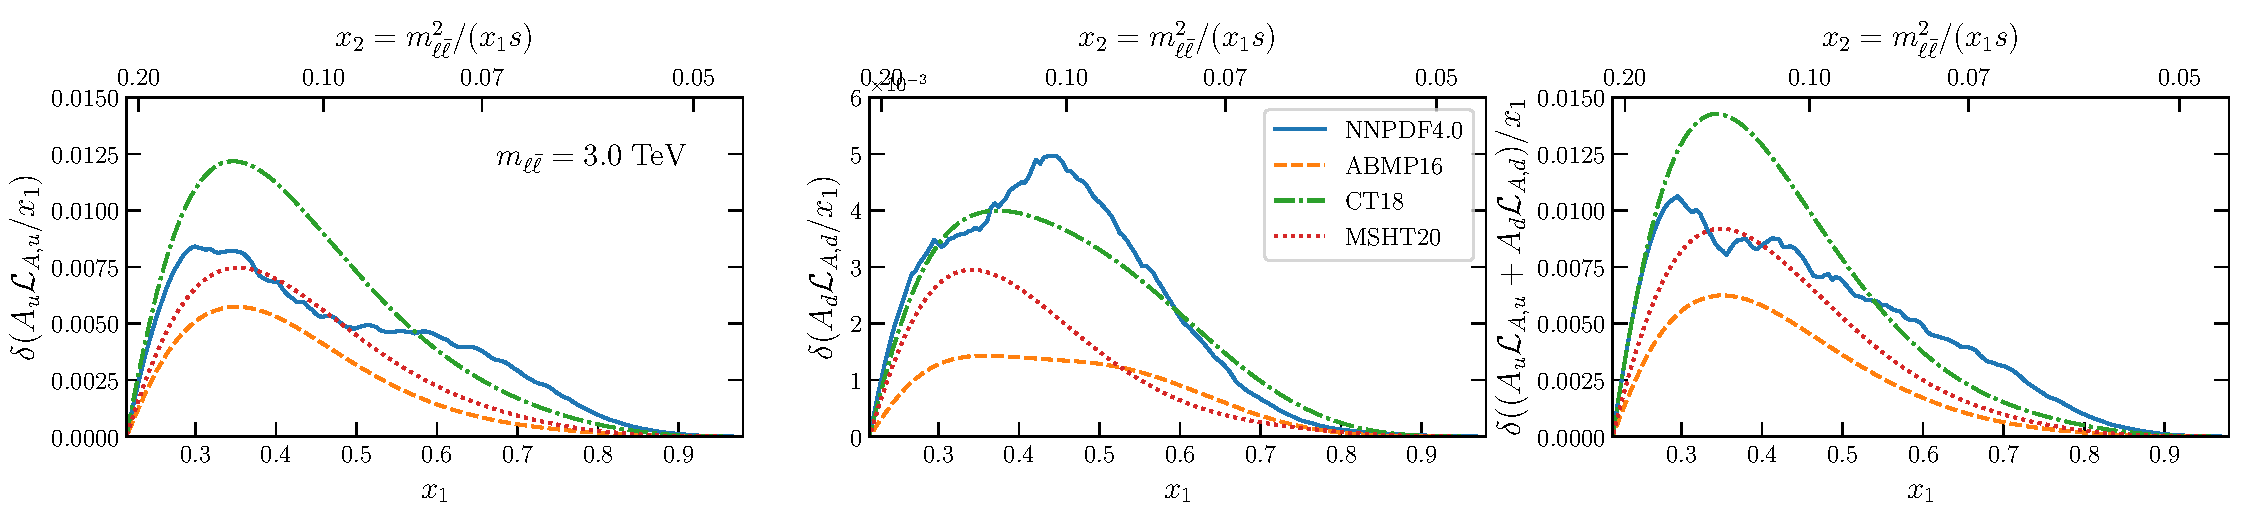
\includegraphics[width=1.00\linewidth]{ch-afb/pdfplot-abs-jacobian-DYlumis-pdfsets-minus-q3p0tev-pdferrs.pdf}
 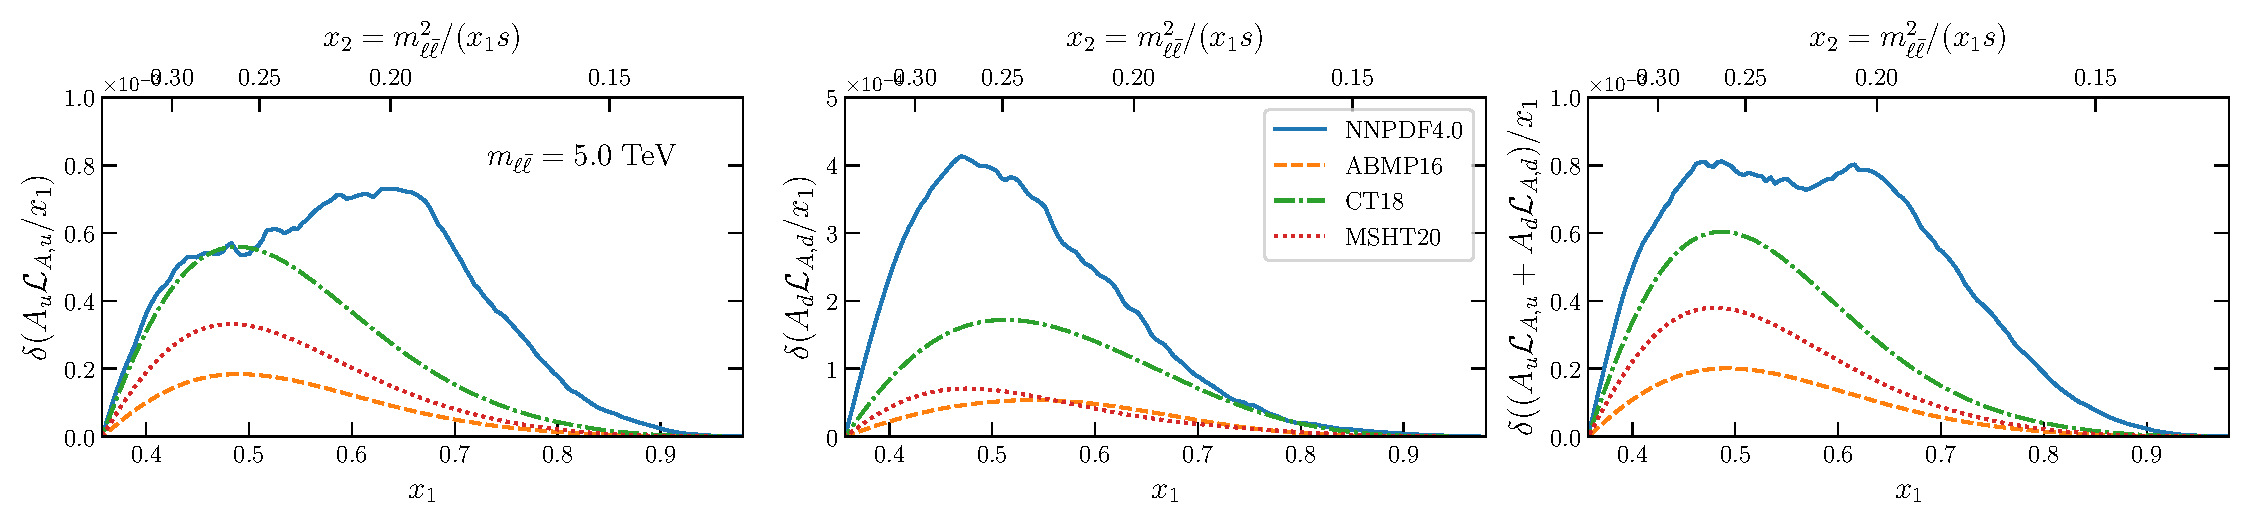
\includegraphics[width=1.00\linewidth]{ch-afb/pdfplot-abs-jacobian-DYlumis-pdfsets-minus-q5p0tev-pdferrs.pdf}
 \caption{Same as Fig.~\ref{fig:mll_dep_lumi_minus} now for the absolute \pdf uncertainties.
    }    
 \label{fig:mll_dep_lumi_minus_pdferrs}
\end{figure}
%---------------------------------------------------------------------------

Fig.~\ref{fig:mll_dep_lumi_minus} shows that for ABMP16, CT18, and
MSHT20 the antisymmetric
parton luminosities depend only mildly on $\mll$, whereas for \nnpdfr{4.0}
they exhibit a strong $\mll$ dependence.
%
Indeed, for dilepton invariant masses of $\mll=3$ TeV there is good
agreement between the three groups, but
for $\mll=5$ TeV the \nnpdfr{4.0} up quark luminosity, while preserving a
similar valence-like shape, is suppressed
by a factor 2 in comparison  to other groups, and the down quark luminosity becomes compatible with zero with a negative
central value,  as already noted. 
%
For all \pdf sets and  $\mll$ values the weighted sum is dominated by the up quark contribution.
The strong scale dependence of $\mathcal{L}_{A,q}$ in \nnpdfr{4.0}
reflects the underlying \pdf behavior seen in  Fig.~\ref{fig:mll_dep_pdfs}
and highlighted by the effective exponents Fig.~\ref{fig:asy_exponents}.
%
As the scale $\mll$ increases, a range of increasingly large $x$ values is probed,
for which, in the case of
\nnpdfr{4.0}, the quark effective exponent slowly increases and the
antiquark exponent rapidly drops.
%
This leads to a negative asymmetry, 
following  Eq.~(\ref{eq:signas}). 

A comparison of the corresponding \pdf uncertainties, displayed in
Fig.~\ref{fig:mll_dep_lumi_minus_pdferrs}, clearly shows the transition
from the data region to the extrapolation region.
%
For
$\mll=3$~TeV the uncertainty $\delta \mathcal{L}_{A,u}$ is generally
small for all sets, with CT18
showing a somewhat larger uncertainty for the up quark, and comparable
uncertainties for the down quark for all \pdf sets.
%
As the scale  increases to $\mll=5$~TeV, where the large-$x$ region is
probed,  the uncertainty 
increases, though more markedly for \nnpdfr{4.0}.
%
For all \pdf sets but
\nnpdfr{4.0}, the
uncertainty is approximately unchanged when the scale is further increased,
while for \nnpdfr{4.0} it grows markedly.

Finally, in Fig.~\ref{fig:asym_coeff_mlldep} we display for all
\pdf sets the
ratio of antisymmetric to symmetric couplings
\be
\label{eq:coupling_ratio}
R_{\rm fb}\equiv \frac{\sum_q g_{A,q}}{\sum_{q'} g_{S,{q'}}} \, ,
\ee
that, according to
Eq.~(\ref{eq:afb_lo}), determines at leading order
the sign and magnitude
of the forward-backward asymmetry distribution $A_{\rm fb}(\cos\theta^*)$.
%
The symmetric and antisymmetric coefficients are obtained by integrating
the corresponding symmetric $\mathcal{L}_{S,q}$ and antisymmetric
$\mathcal{L}_{A,q}$ partonic luminosities according to
Eq.~(\ref{eq:gAq_integrated_1}), and the result is shown as a function of the lower integration cut $\mll^{\rm min}$.
%
In all cases the correlation between \pdf uncertainties in the numerator and
the denominator are kept into account.

%-------------------------------------------------------------------------------
\begin{figure}[!t]
 \centering
 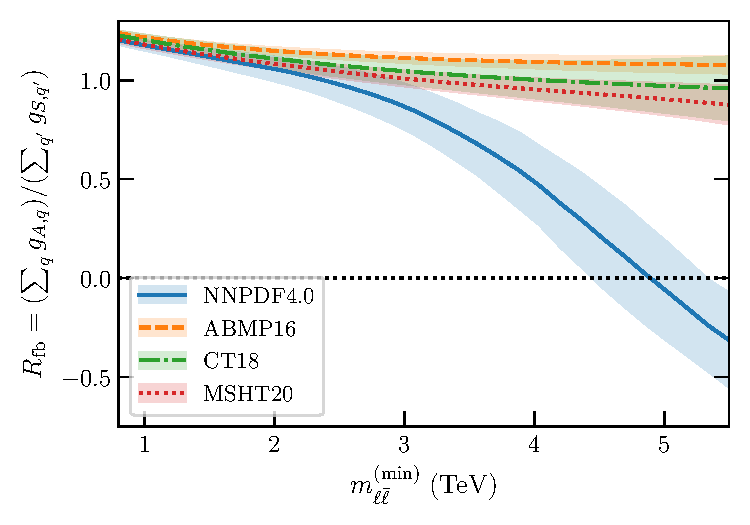
\includegraphics[width=0.60\linewidth]{ch-afb/asym_coeff_mlldep.pdf}
 \caption{The coupling ratio $R_{\rm fb}$,
   Eq.~(\ref{eq:coupling_ratio}),
   that enters the forward-backward asymmetry $A_{\rm
     fb}(\cos\theta^*)$ at \lo,  Eq.~(\ref{eq:afb_lo}), for different \pdf
   sets, as  a function of the lower cut in the dilepton
   invariant mass $\mll^{\rm min}$.
 }    
 \label{fig:asym_coeff_mlldep}
\end{figure}
%---------------------------------------------------------------------------

Fig.~\ref{fig:asym_coeff_mlldep} shows that, consistently
with the behavior of the luminosity of
Fig.~\ref{fig:mll_dep_lumi_minus},  for $\mll^{{\rm
    min}}\lsim 3$~TeV results agree within uncertainties for all \pdf
sets.
%
The situation is different for higher dilepton invariant masses $\mll^{{\rm min}}\gsim 3$~TeV:
the ratio $R_{\rm fb}$ starts to decrease for \nnpdfr{4.0}, while it
remains approximately  constant 
for the other  \pdf sets. In particular, for \nnpdfr{4.0} the coupling ratio
vanishes around $\mll^{{\rm min}}\sim5$~TeV, and it becomes negative
for yet larger   $\mll^{{\rm min}}$ values.
It follows that the forward-backward
asymmetry in high-mass Drell-Yan production should decrease  and
eventually vanish (and possibly even turn negative)
in \nnpdfr{4.0} as the $\mll^{{\rm min}}$ cut is increased,
while for CT18, MSHT20, and ABMP16 it should remain positive
with a similar magnitude irrespective of the cut  $\mll^{{\rm min}}$ adopted.

%-------------------------------------------------------------------------------
\begin{figure}[!t]
 \centering
 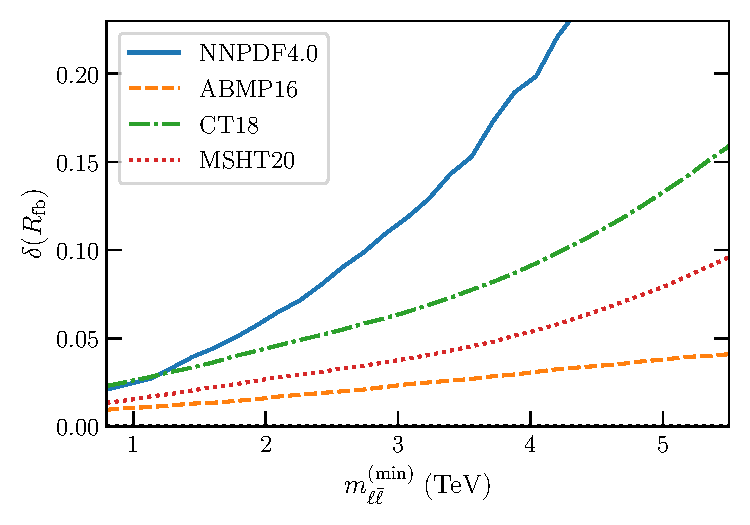
\includegraphics[width=0.49\linewidth]{ch-afb/asym_coeff_mlldep_abserr.pdf}
 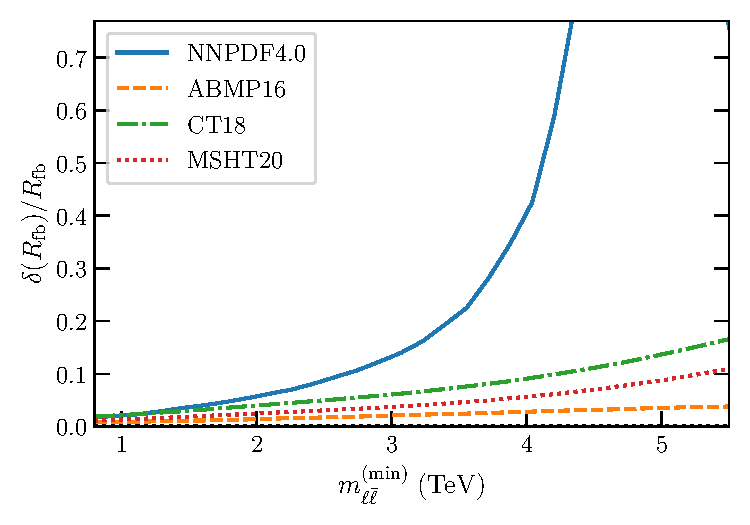
\includegraphics[width=0.49\linewidth]{ch-afb/asym_coeff_mlldep_relerr.pdf}
 \caption{The absolute (left) and relative (right panel) uncertainties
   in the coupling ratio $R_{\rm fb}$ shown in Fig.~\ref{fig:asym_coeff_mlldep}.
 }    
 \label{fig:asym_coeff_mlldep_err}
\end{figure}
%---------------------------------------------------------------------------

Fig.~\ref{fig:asym_coeff_mlldep_err} displays the 
absolute  and relative  uncertainties
associated to the coupling ratio $R_{\rm fb}$.
%
We observe that \nnpdfr{4.0} shows
the most marked increase of the uncertainties in $R_{\rm fb}$
as $\mll^{\rm min}$ grows.
%
For instance, for  $\mll^{\rm min}\gtrsim4$~TeV
the absolute \pdf uncertainty in \nnpdfr{4.0}
is about twice as large as that found using CT18 
four times as large as MSHT20,
and about one order of magnitude larger than ABMP16.
%
This trend is magnified for the relative uncertainties
due to the decrease in the central value of $R_{\rm fb}$
as $\mll^{\rm min}$ increases.


\section{The Drell-Yan forward-backward asymmetry at the \lhc}
\label{sec:afb/afb}
% % !TeX root = ../../../main.tex

After the qualitative discussion of the previous sections, here we
present results for the $\cos\theta^*$
distributions \cref{eq:afb/dsigma-dcos} and the
forward-backward asymmetry \cref{eq:afb/forward-backward-asymmetry}, with
\nlo QCD and electroweak corrections included and
with realistic selection and acceptance cuts for the \lhc at $\sqrt{s} = 14$~TeV
and different values of the invariant mass $\mll$ relevant for SM
studies and \bsm searches.

Computations are performed using \mgamc~\cite{Alwall:2014hca},
interfaced to \pineappl~\cite{Carrazza:2020gss,christopher_schwan_2022_7023438} to generate
fast interpolation grids.
%
In order to account for realistic detector acceptances,
we impose phase-space cuts on the transverse momentum and the pseudo-rapidity of the two
leading leptons,
\be
p_T^{\ell} > 10~{\rm GeV}  \, ,\qquad |\eta_{\ell}| < 2.4 \,.
\ee
We then consider various regions of dilepton invariant mass $\mll$:
either close to the $Z$-boson peak ($60$~GeV $< \mll < 120$~GeV),
relevant for precision SM studies, or the
high-mass region relevant for \bsm searches, with  various choices of a
lower mass invariant cutoff ($\mll > 3,4,5,6$~TeV).
%
In all cases, in order to facilitate the interpretation of
hadron-level results  and the connection to
the discussion of the \pdf features from \cref{sec:afb/largexpdfs},
we also provide results for the two partonic channels that give the
largest contribution to the cross-section.
%
As in \cref{sec:afb/largexpdfs}, we compare results obtained using
the  ABMP16, CT18, MSHT20, and \nnpdfr{4.0} \pdf sets.
%
In all cases, we
use the  \nnlo sets corresponding to the value $\alpha_s(m_Z)=0.118$
of the strong coupling.
%
Results obtained using the NNPDF3.1 \pdf set are reported in App.~\ref{app:nnpdf31}.

%-------------------------------------------------------------------------------
\begin{figure}[!t]
 \centering
 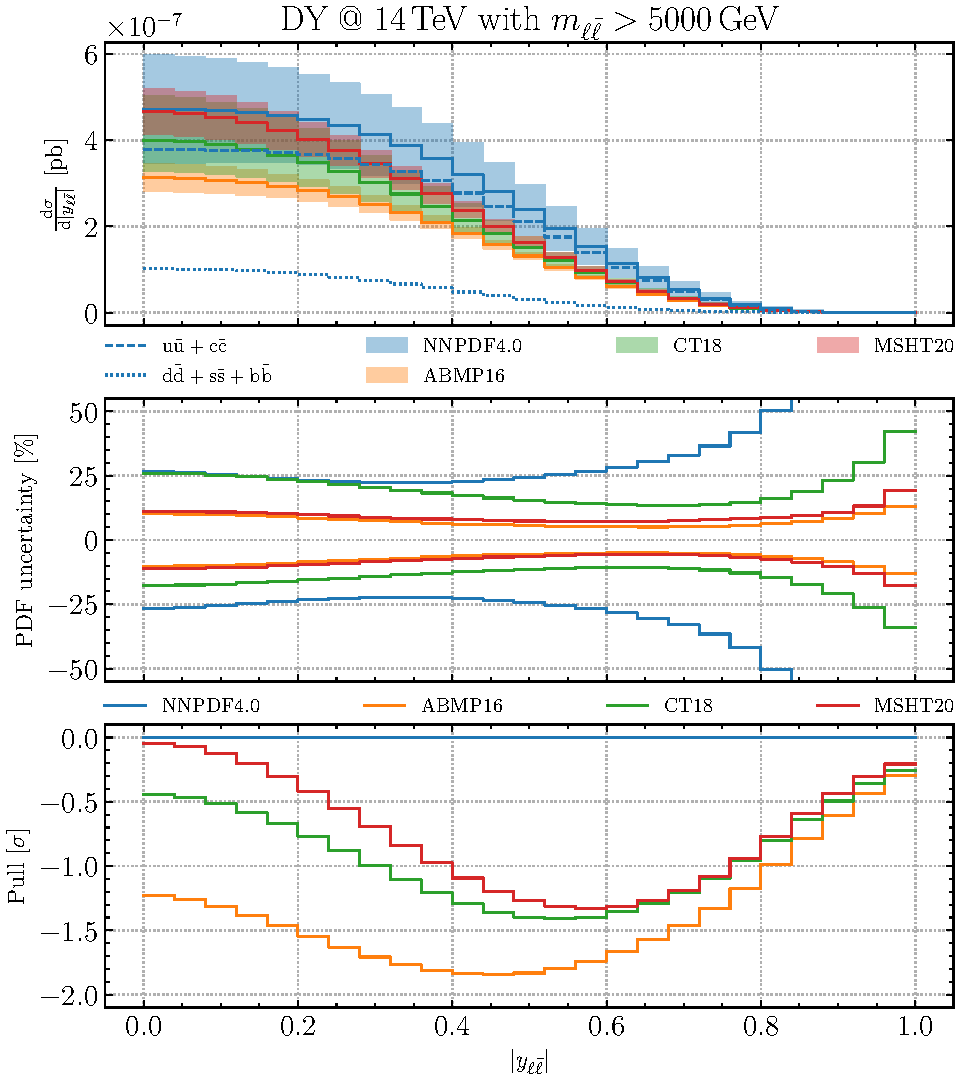
\includegraphics[width=0.49\linewidth]{ch-afb/NNPDF_DY_14TEV_BSM_AFB_YLL_5000}
 \caption{The differential distribution in absolute dilepton rapidity $|\yll|$, given in
\cref{eq:afb/dsigma-dyll},
for dilepton invariant masses of $\mll > 5$~TeV
for neutral current Drell-Yan production at the
\lhc 14 TeV,
obtained using ABMP16, CT18, MSHT20, and \nnpdfr{4.0} \nnlo \pdfs with $\alpha_s(m_Z)=0.118$.
%
All
uncertainties shown are 68\% CL \pdf uncertainties, computed at \nlo
in the QCD and EW couplings with realistic cuts (see text).
We show the absolute distributions (top), relative uncertainties (normalized
to the central curve of each set, middle) and the pull with respect to the
\nnpdfr{4.0} result, \cref{eq:afb/pulldef_xsec} (bottom).
%
For the central \nnpdfr{4.0} prediction
the contributions of the $u\bar{u}+c\bar{c}$ and $d\bar{d}+s\bar{s}+b\bar{b}$
parton subchannels are also shown.
 \label{fig:afb/CMS_DY_14TEV_MLL_5000_rap}}
\end{figure}
%-------------------------------------------------------------------------------

Before considering the angular distributions, in
\cref{fig:afb/CMS_DY_14TEV_MLL_5000_rap} we display the 
differential distribution in absolute dilepton rapidity $|\yll|$,
defined in \cref{eq:afb/dsigma-dyll},
for a dilepton invariant mass of $\mll > 5$~TeV.
%
This is the kinematic region relevant for searches of high-mass resonances
in the dilepton channel at the \lhc, e.g.~\cite{ATLAS:2019erb,Khachatryan:2016zqb}.
%
We display the absolute differential distributions with the 68\% CL \pdf uncertainties
(top), the relative \pdf uncertainty (center) normalized for each \pdf
set to the corresponding central prediction, and the pull between the
\nnpdfr{4.0} result, taken as a reference, and other sets (bottom).
%
This pull is    defined as
    \be
\label{eq:afb/pulldef_xsec}
{\rm Pull}_i= \frac{ \sigma^{(0)}_{2,i} -\sigma^{(0)}_{1,i} }{
  \sqrt{ \lp  \delta \sigma_{2,i}\rp^2+\lp  \delta \sigma_{1,i}\rp^2 }} \, , \qquad i=1,\ldots,n_{\rm bin} \, ,
\ee
where  $\sigma^{(0)}_{1,i}$ and $\sigma^{(0)}_{2,i}$ are the central values of the
theory prediction in the $i$-th bin of the distribution and $\delta \sigma_{1,i}$, $\delta \sigma_{2,i}$ are
the corresponding \pdf uncertainties.
%
For the central \nnpdfr{4.0} prediction in the upper panel we also display the
contributions from the dominant parton subchannels, namely
$u\bar{u}+c\bar{c}$ and $d\bar{d}+s\bar{s}+b\bar{b}$.

As discussed in \cref{sec:afb/HMDY}, the  $|y_{\ell\bar{\ell}}|$  distribution
depends  on the symmetric partonic luminosities $\mathcal{L}_{S,q}$, \cref{eq:afb/lumiss_qpm},
which in turn are driven by the total \pdfs $xf^+_q$.
%
The $|y_{\ell\bar{\ell}}|$  distribution
is dominated by the $u\bar{u}$
contribution and its qualitative behaviour is found to be similar for the four \pdf sets considered.
%
\pdf uncertainties are the largest in \nnpdfr{4.0}, ranging between 25\% and 50\%,
and the pull between \nnpdfr{4.0} and  CT18 and MSHT20 is at most at the
$1.5\sigma$ level, and slightly larger  
with ABMP16.
%
The dependence of the $|y_{\ell\bar{\ell}}|$  distribution on the dilepton mass $\mll$
is moderate, and the same qualitative features are
obtained if $\mll$ is lowered down to the $Z$-peak region, or
raised to yet higher values.
%
Hence, for the absolute rapidity distribution there is a
reasonable agreement between all  \pdf sets for all scales considered.

%-------------------------------------------------------------------------------------
\begin{figure}[t]
\centering
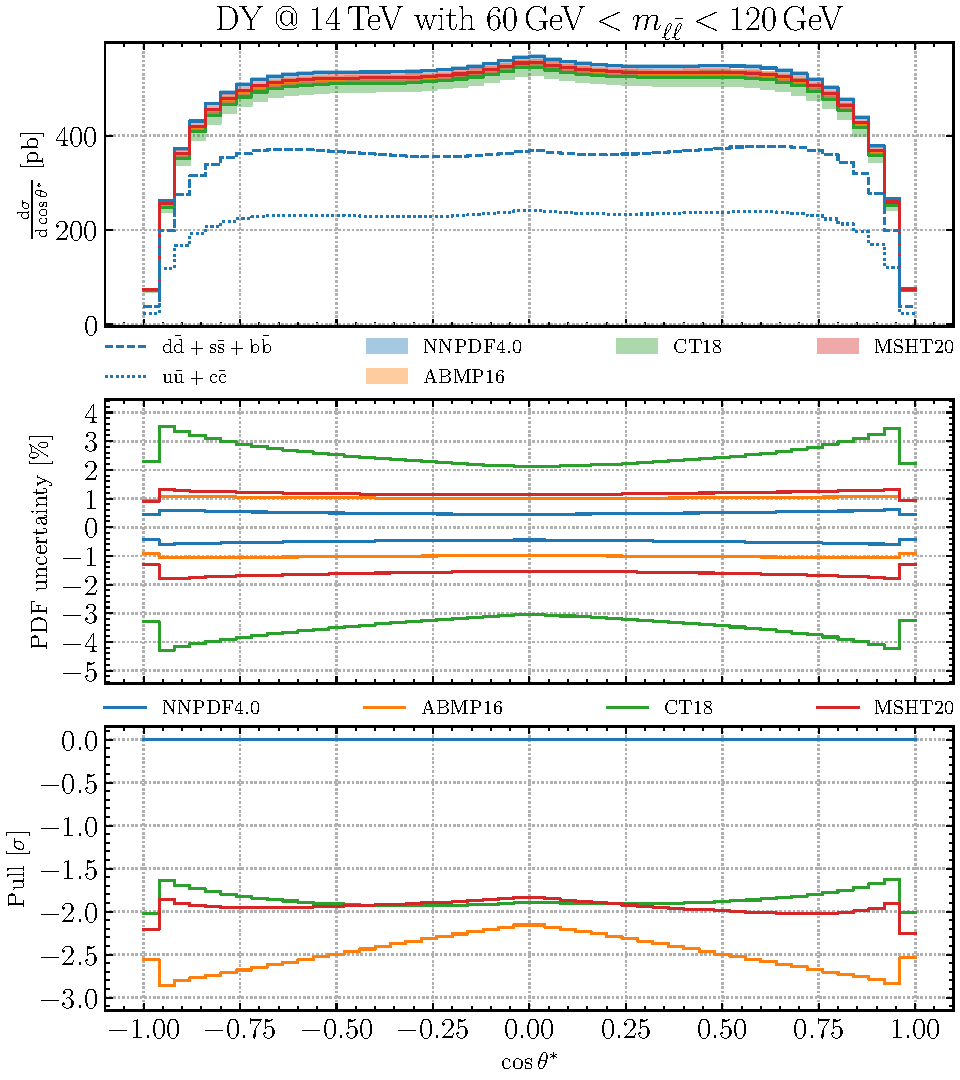
\includegraphics[width=0.49\linewidth]{ch-afb/NNPDF_DY_14TEV_BSM_AFB_COS_060_120}
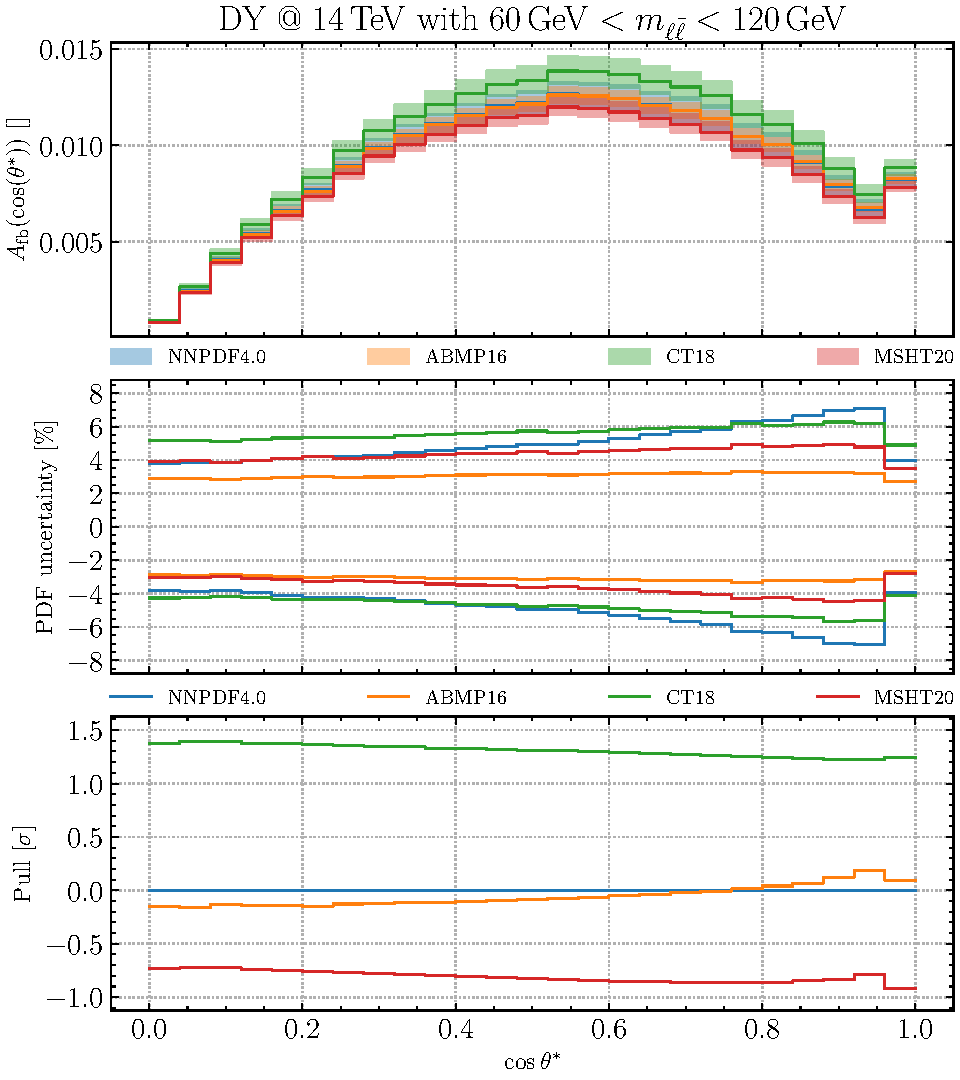
\includegraphics[width=0.49\linewidth]{ch-afb/NNPDF_DY_14TEV_BSM_AFB_COS_060_120-afb}
\caption{Same as \cref{fig:afb/CMS_DY_14TEV_MLL_5000_rap}, now for the differential distribution in
  $\cos\theta^*$ (left)
  and the corresponding forward-backward asymmetry
  $A_{\rm fb}(\cos\theta^*)$ (right), in the $Z$-peak region defined by $60~{\rm GeV} < \mll < 120$ GeV.}
\label{fig:afb/CMS_DY_14TEV_MLL_zpeak}
\end{figure}
%-------------------------------------------------------------------------------------

We now turn to the differential distribution in
  $\cos\theta^*$ 
  and the corresponding forward-backward asymmetry $A_{\rm
    fb}(\cos\theta^*)$.
We first consider the $Z$-peak region, $60~{\rm GeV} < \mll <
120$~GeV, in \cref{fig:afb/CMS_DY_14TEV_MLL_zpeak}.
%
The $\cos\theta^*$ 
distribution exhibits a small but non-negligible asymmetry,
and uncertainties are  smallest for \nnpdfr{4.0}.
%
The four \pdf sets predict a similar behaviour and magnitude
of the asymmetry $A_\mathrm{fb}$.
%
\pdf uncertainties in the asymmetry
are  comparable for  all \pdf sets when $\cos\theta^* \approx0$,
and actually  largest for \nnpdfr{4.0} when $\cos\theta^* \approx 1$.
In all cases the predictions are compatible within $2 \sigma$,
with ABMP16 showing larger differences of up to $2.8 \sigma$ for the $\cos\theta^*$
distribution.
%
Note that the
sharp drop-off at the edges $|\cos\theta^*| \approx  1$, appearing in
all plots in this section, is a consequence of the phase-space cuts which
limit the phase-space volume.
%
Indeed, using  \lo kinematics
\begin{equation}
| \cos\theta^* | = \tanh \left| \frac{\eta_\ell - \eta_{\bar{\ell}}}{2} \right| = \sqrt{1 - \frac{4 (p_T^\ell)^2}{\mll^2}} \text{,}
\end{equation}
so $| \cos\theta^* | \approx 1$ requires a lepton pair with either
a large rapidity separation, or a very large invariant mass and small
transverse momenta. 

As expected from the antisymmetric partonic luminosities studied in
\cref{subsec:afb/partoniclumis}, the situation is quite different when
considering distributions with a higher dilepton invariant mass range.
%
The angular distribution and forward-backward asymmetry
in the high-mass region, for different values of the  lower cut in the dilepton
 invariant mass, namely $\mll^{\rm min}=3, 4,5$ and 6 TeV, are
 respectively
 shown in
\cref{fig:afb/CMS_DY_14TEV_MLL_others} and \cref{fig:afb/CMS_DY_14TEV_MLL_others_asy}.

%-------------------------------------------------------------------------------
\begin{figure}[t!]
 \centering
 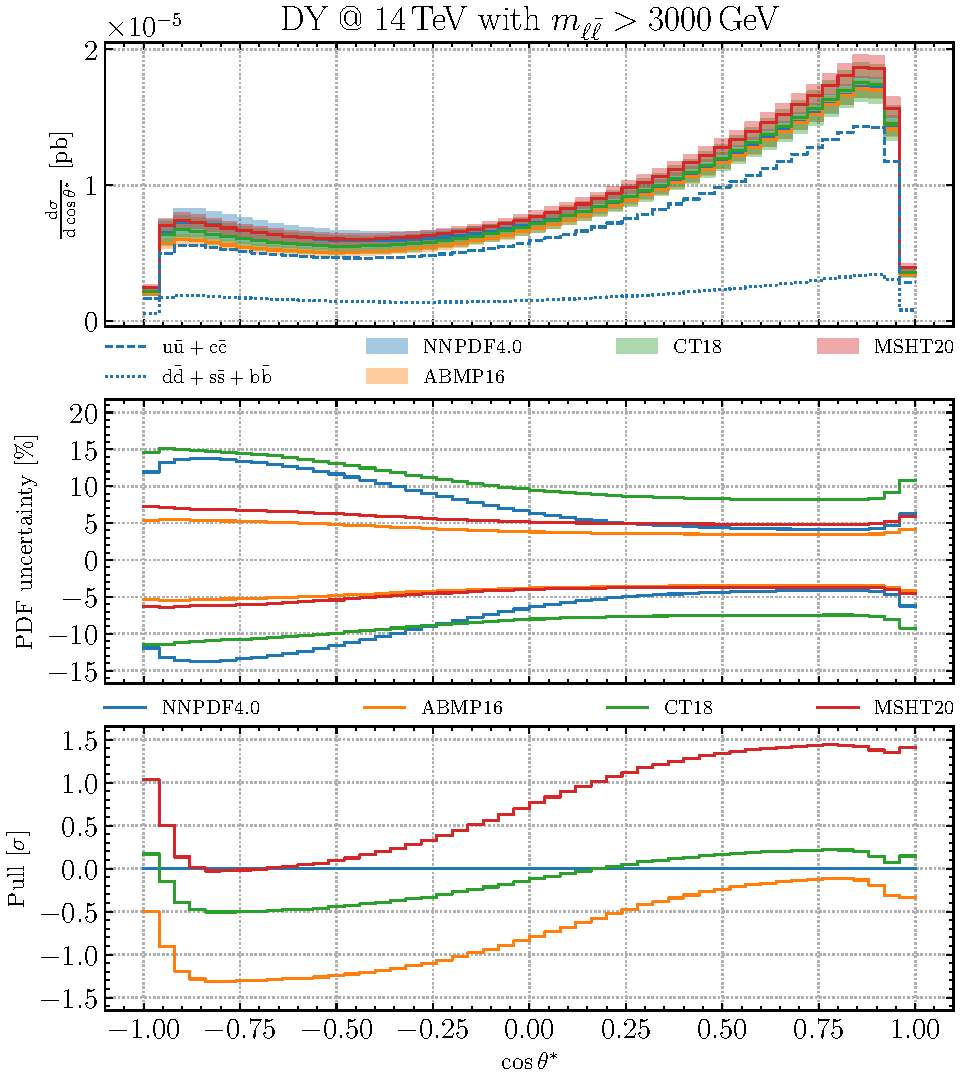
\includegraphics[width=0.49\linewidth]{ch-afb/NNPDF_DY_14TEV_BSM_AFB_COS_3000}
 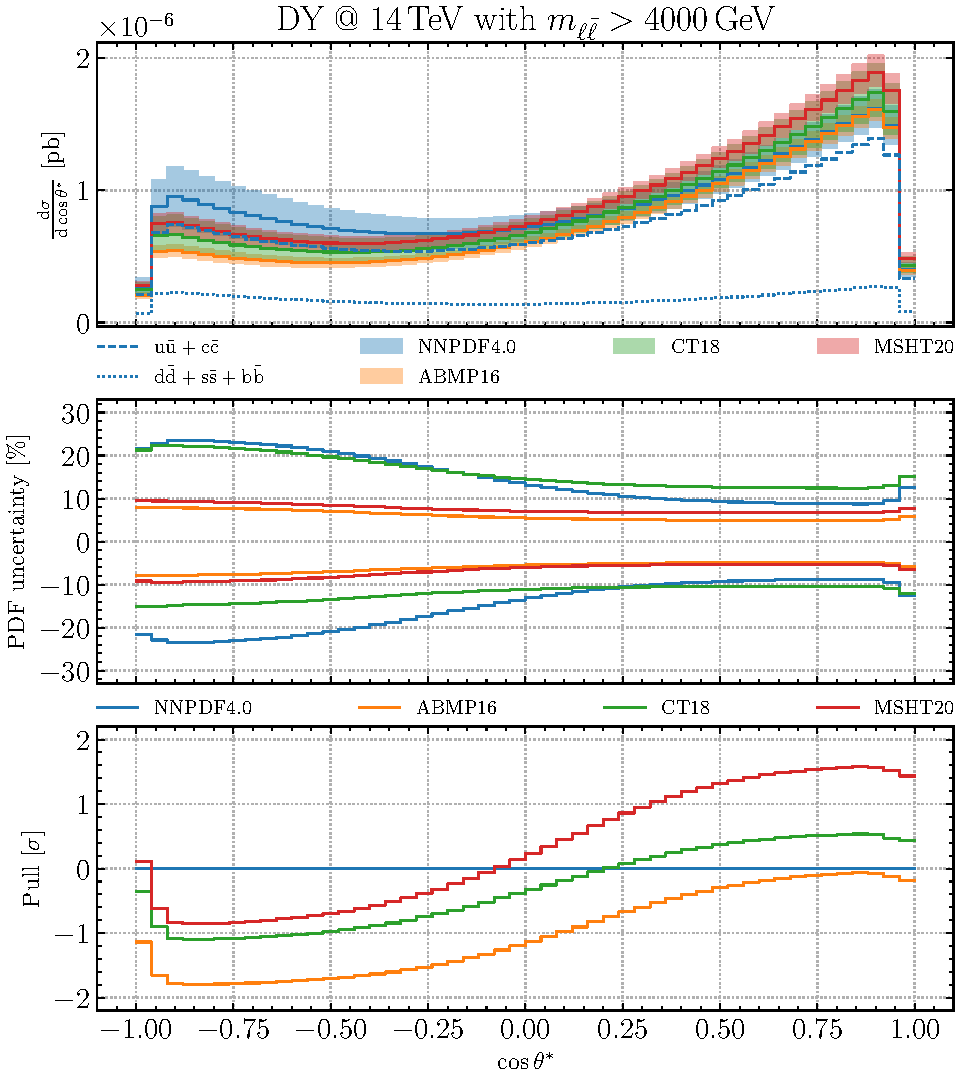
\includegraphics[width=0.49\linewidth]{ch-afb/NNPDF_DY_14TEV_BSM_AFB_COS_4000}
 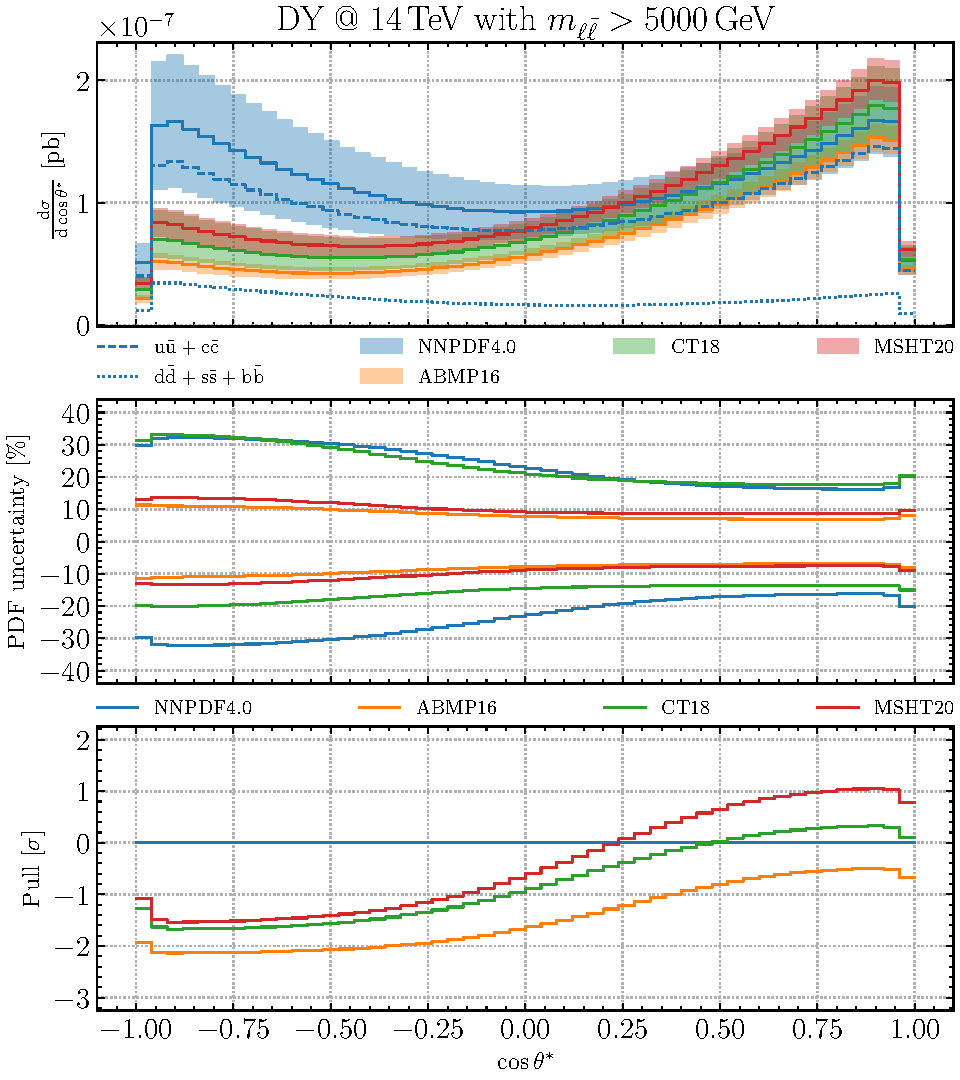
\includegraphics[width=0.49\linewidth]{ch-afb/NNPDF_DY_14TEV_BSM_AFB_COS_5000}
 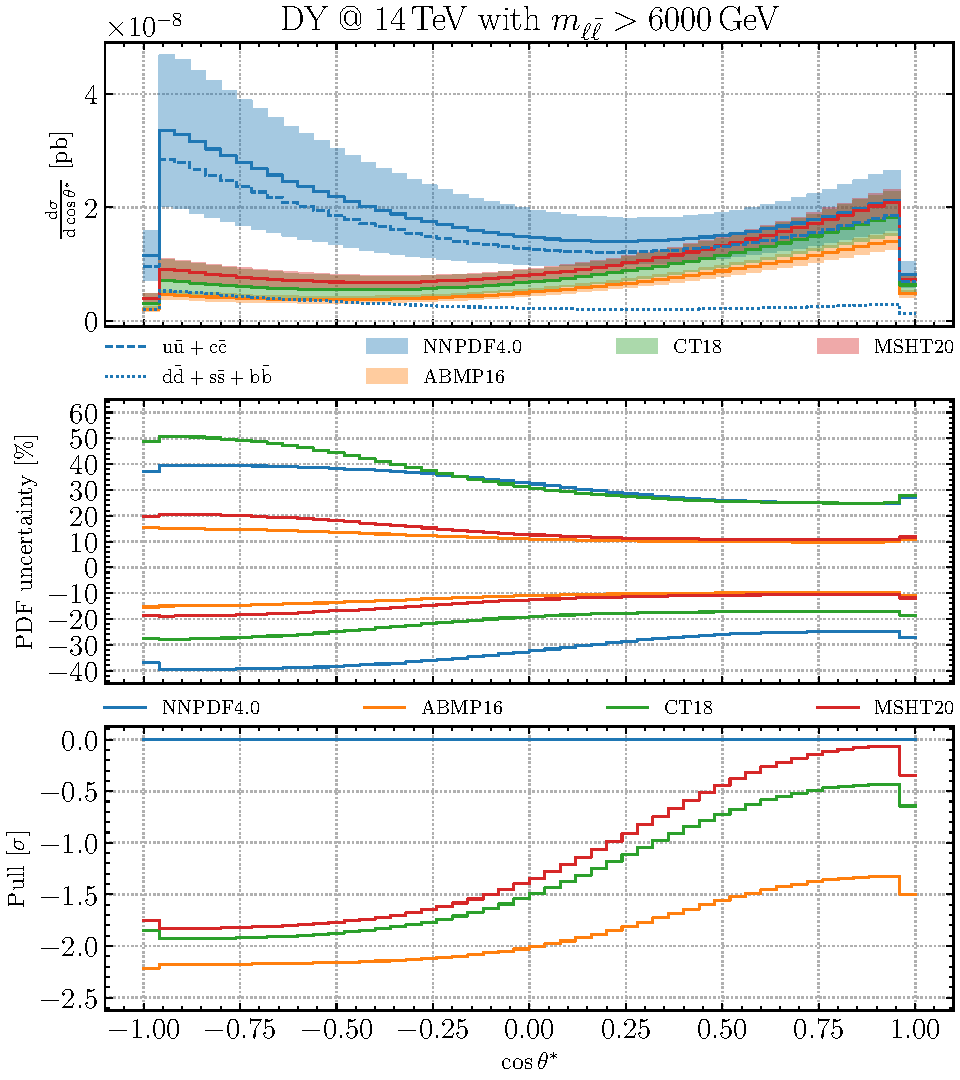
\includegraphics[width=0.49\linewidth]{ch-afb/NNPDF_DY_14TEV_BSM_AFB_COS_6000}
 \caption{Same as \cref{fig:afb/CMS_DY_14TEV_MLL_zpeak} (left)
   for different values of the  lower cut in the dilepton
   invariant mass: $\mll \ge 3, 4,5,$ and 6 TeV respectively.
  }    
 \label{fig:afb/CMS_DY_14TEV_MLL_others}
\end{figure}
%-------------------------------------------------------------------------------

 Consistent with the underlying parton luminosities, the $\cos\theta^*$ distribution
 is dominated by $u\bar{u}$ scattering, while  $d\bar{d}$ provides
 a subdominant contribution.
 %
 When the lower cut  is $\mll^{(\rm min)}=3$ TeV is used, the four \pdf
 sets are in agreement at the $1\sigma$ level: they all
 display a 
 positive forward-backward asymmetry, and exhibit \pdf uncertainties ranging between 10\% and 15\%.
 %
 As the invariant mass cut is raised, the qualitative behaviour of the
 angular distribution and
 asymmetry change substantially for \nnpdfr{4.0}, while they remain
 approximately the same for all other \pdf sets, consistent with the
 behaviour of the \pdfs and luminosities discussed in
 \cref{sec:afb/subsec-largexPDFs}-\ref{subsec:partoniclumis}.
%
 Specifically,
 raising the cut to
 $\mll \ge 4$ TeV, for \nnpdfr{4.0}
 the backwards cross-section starts increasing, though the asymmetry remains
positive.
 %

For $\mll\ge 5$ TeV the central value of the \nnpdfr{4.0} $\cos\theta^*$
 distribution  becomes symmetric, though the  \pdf uncertainty band is
 rather asymmetric. Also, \pdf uncertainties
 are now the largest for \nnpdfr{4.0}, reaching up to 30\%.
 %
 Finally, for $\mll\ge 6$ TeV  the central value of 
 forward-backward asymmetry for \nnpdfr{4.0} becomes negative, with the
 \pdf uncertainties increasing further so the asymmetry remains compatible
 with zero at about the 1.1~$\sigma$ level.
   %
 For all other \pdf sets there is little change in the shape of the distribution as the
 dilepton invariant mass cut is increased.

%-------------------------------------------------------------------------------
\begin{figure}[t!]
 \centering
 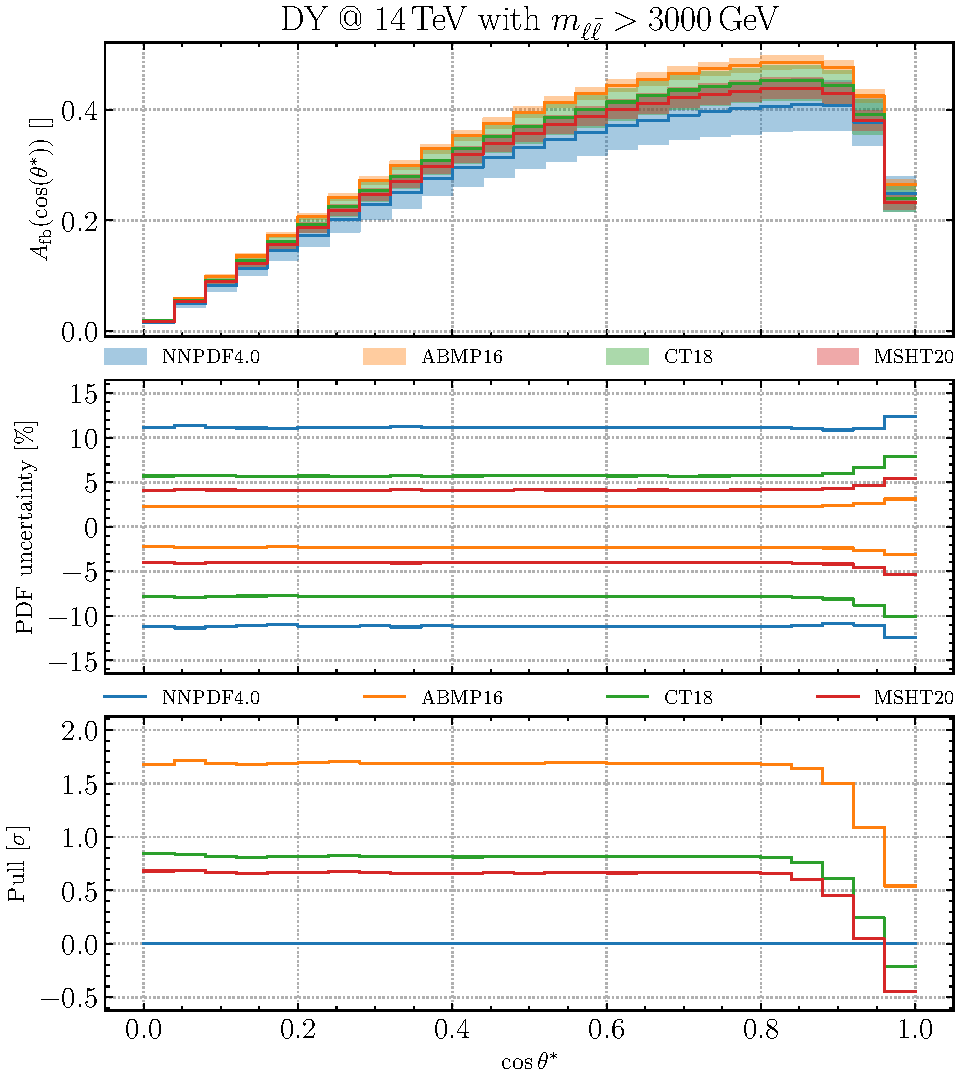
\includegraphics[width=0.49\linewidth]{ch-afb/NNPDF_DY_14TEV_BSM_AFB_COS_3000-afb}
 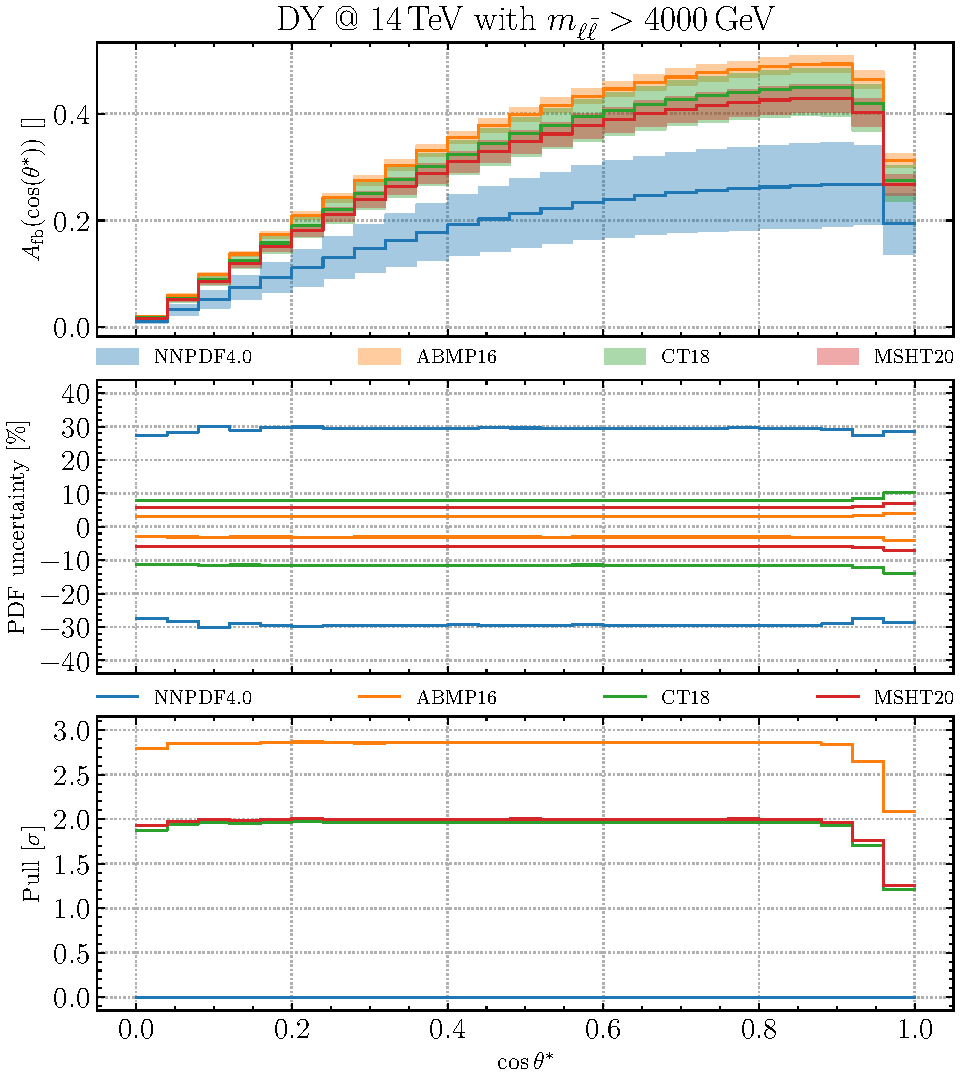
\includegraphics[width=0.49\linewidth]{ch-afb/NNPDF_DY_14TEV_BSM_AFB_COS_4000-afb}
 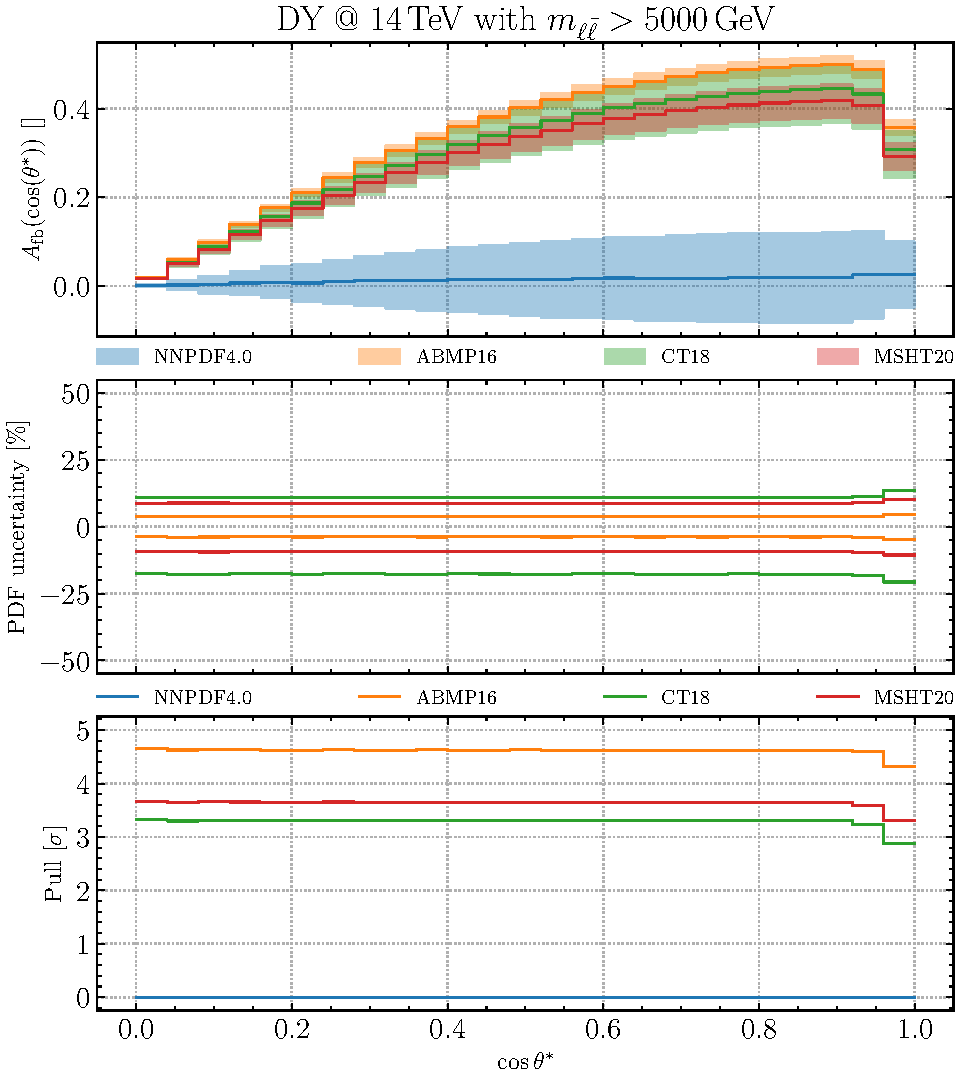
\includegraphics[width=0.49\linewidth]{ch-afb/NNPDF_DY_14TEV_BSM_AFB_COS_5000-afb}
 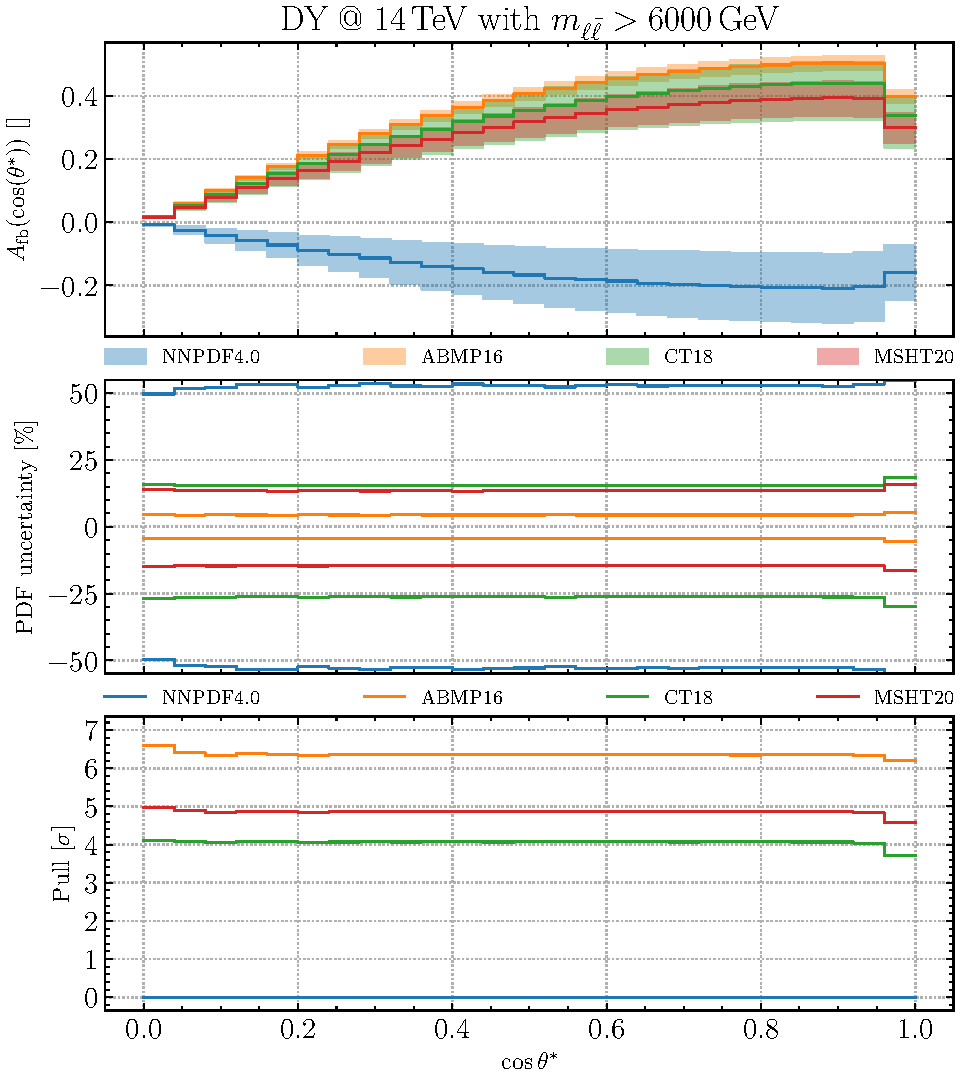
\includegraphics[width=0.49\linewidth]{ch-afb/NNPDF_DY_14TEV_BSM_AFB_COS_6000-afb}
 \caption{Same as \cref{fig:afb/CMS_DY_14TEV_MLL_zpeak} (right)
   for different values of the  lower cut in the dilepton
   invariant mass: $\mll^{\rm min}=3, 4,5,$ and 6 TeV.
  }    
 \label{fig:afb/CMS_DY_14TEV_MLL_others_asy}
\end{figure}
%-------------------------------------------------------------------------------

Because of the very large uncertainty on the \nnpdfr{4.0} result for the $\cos\theta^*$
distribution, even with
the highest value of the  $\mll^{(\rm  min)}$ cut, where \nnpdfr{4.0} finds a
symmetric distributions while all other \pdf sets find an asymmetry,
the pull is always below $2 \sigma$.
%
This suggests that the more
conservative estimate of  \nnpdfr{4.0} in the extrapolation region might be
desirable, and lead to more robust predictions for the
forward-backward asymmetry in the high-mass region which is relevant
for new physics searches.


\section{Summary and outlook}
\label{sec:afb/summary}
% % !TeX root = ../../../main.tex

In this work we have scrutinised the \pdf dependence of  neutral current
Drell-Yan production
at large dilepton invariant masses $\mll$, focusing on the behavior
of the forward-backward asymmetry $A_{\rm fb}$
in the Collins-Soper angle $\cos\theta^*$, an observable frequently
considered in the context of searches for new physics beyond the SM.
%
We have demonstrated that while theoretical
predictions for the sign and magnitude of $A_{\rm fb}$ are very
similar for all \pdf sets in the
$Z$ peak region, they
depend markedly on the choice of \pdf set for  large values of $\mll$. 
We have traced this behavior to that of the \pdfs, which agree in the
data region, but differ in the large-$x$
region, where \pdfs are mostly unconstrained by data.

We have specifically shown that the uncertainty on the asymmetry
differs substantially between \pdf sets, with \nnpdfr{4.0} displaying
a more marked increase as  $\mll$ grows, leading to
an absolute uncertainty that e.g.\ for $\mll^{\rm min}\gtrsim4$~TeV
is about twice as large as that found using CT18, 
four times as large as MSHT20,
and about one order of magnitude larger than ABMP16.
%
Also, whereas other \pdf sets predict a shape of the asymmetry
which is unchanged when  $\mll$ increases from the $Z$-peak region to
the TeV range, namely a 
positive
asymmetry implying a larger cross-section  for $\cos\theta^*\ge 0$, \nnpdfr{4.0} finds that as
$\mll$ increases, the asymmetry is reduced, and the $\cos\theta^*$ distribution
becomes symmetric when $\mll^{\rm min}\sim5$~TeV.

We have traced this behavior to that of the underlying
\pdfs in the large-$x$ region, where \pdfs are mostly unconstrained by
data.
%
Specifically we have seen that in this region \nnpdfr{4.0} has
generally wider uncertainties.
%
Also, while for  all \pdf  sets the
quark and antiquark distributions vanish as
a power of $(1-x)$ as $x\to 1$, for all groups but \nnpdfr{4.0} this power is
constant for light quarks to the right of the valence peak, while for
\nnpdfr{4.0} it changes as $x$ increases, slowly for up quarks, more rapidly
for down quarks and even more rapidly for antiquarks.
%
All this suggests that the different behavior of
\nnpdfr{4.0} is due to its more flexible \pdf parametrization.

Our general conclusion is that the 
behavior of the forward-backward asymmetry
observed at lower invariant masses is not necessarily reproduced at
large masses if flexible enough
\pdfs are used:  the characteristic positive asymmetry observed
for low $\mll$ values
can be washed out in the high-mass region.
%
Hence, deviations from the traditional expectation of a positive forward-backward
asymmetry in high-mass Drell-Yan cannot be taken as an indication of 
\bsm physics,
at least based on  our current understanding of proton structure in the large-$x$ region.

Turning the argument around, future measurements of the $\cos\theta^*$
distribution and the associated forward-backward asymmetry 
$A_{\rm fb}$ when included in \pdf determinations could help in
constraining \pdfs at large $x$.
%
For instance, Fig.~\ref{fig:CMS_DY_14TEV_MLL_others} indicates that for
$\mll^{\rm min}=5$ TeV and $\sqrt{s}=14$ TeV the
asymmetry $A_{\rm fb}$ can be as large as 50\% for ABMP16
while it vanishes (within large uncertainties) in the case of \nnpdfr{4.0}.
%
By rebinning the $\cos\theta^*$ distribution, for an integrated
luminosity of $\mathcal{L}=6$ ab$^{-1}$, corresponding to the
combination at ATLAS and CMS 
at the end of the HL-\lhc data-taking period, $\mathcal{O}(10)$ events are expected in the backward region,
with an statistical uncertainty of $\delta_{\rm stat}\sim 30\%$ which could be sufficient to
discriminate between these two limiting scenarios at the $2\sigma$ level.

Higher event counts are expected if the $\mll$ cut is loosened, though one is
then less sensitive to the large-$x$ region where differences between \pdf sets and their
uncertainties are the largest.
%
Ultimately, the constraining power of high-mass Drell-Yan in general and of the forward-backward
asymmetry in particular can only be addressed by means of a dedicated projections
based on binned pseudo-data such as those carried
out for the HL-\lhc and the Electron Ion Collider in e.g.~\cite{AbdulKhalek:2018rok,Khalek:2021ulf}.
%
While we leave this exercise for a future study, the investigations
presented in this work indicate that $A_{\rm fb}$
at high-invariant masses represents a promising and mostly
unexplored channel to pin down large-$x$ light
quark and antiquark \pdfs at the HL-\lhc.

While in this work
we have focused on the forward-backward asymmetry in neutral-current Drell-Yan production,
similar considerations apply for other processes relevant
for \bsm searches at high mass at the \lhc.
%
Indeed, the HL-\lhc will be sensitive to a broad range of hypothetical
new massive particles, from resonances in the $m_{jj}$ dijet invariant mass distribution up to 11 TeV,
heavy vector triplet resonances decaying into a diboson $VV'$ pair up to 5 TeV,
and gluinos with masses up to $m_{\tilde{g}}=3$ TeV in the minimal
supersymmetric standard model (MSSM) with a massless lightest SUSY
particle~\cite{CidVidal:2018eel}.
%
For all these channels, a robust understanding of \pdfs
and their uncertainties at large $x$, including the role of
methodological and model assumptions, will be necessary to fully exploit
the HL-\lhc discovery potential for \bsm signatures.
%
%
Conversely, once \bsm phenomena have been excluded in some high-energy channel,
the corresponding search can be unfolded into a measurement to provide direct
constraints on the \pdfs in this key large-$x$ region, which in turn will
enhance the reach of other searches.

\subsection*{Acknowledgments}

We are grateful to Dimitri Bourilkov, Alexander Grohsjean, Meng Lu, and Jan Schulte for raising with us the issue of the
\pdf dependence of $A_{\rm fb}$ at high invariant masses and for the subsequent discussions.
%
A.~C., S.~F., and F.~H.\ are supported by
the European Research Council under 
the European Union's Horizon 2020 research and innovation Programme
(grant agreement n.740006).
%
R.~D.~B.\ is supported by the U.K.\
Science and Technology Facility Council (STFC) grant ST/P000630/1.
%
E.~R.~N.\ is supported by the Italian Ministry of University and Research (MUR)
through the ``Rita Levi-Montalcini'' Program.
%
J.~R.\ is partially supported by NWO (Dutch Research Council).
%
C.~S.\ is supported by the German Research Foundation (DFG) under
reference number DE~623/6-2.


\section{\texorpdfstring{$A_\text{fb}$}{Afb} in \nnpdfr{3.1}}
\label{app:afb/nnpdf31}
% % !TeX root = ../../../main.tex

In this appendix we compare partonic luminosities
and \lhc differential distributions obtained with \nnpdfr{4.0} in
Sects.~\ref{sec:largexpdfs}
and~\ref{sec:afb} with those based 
on its predecessor
NNPDF3.1, as well as with a variant of \nnpdfr{4.0}
where positivity is imposed at the level of observable cross-sections but
not at the \pdf level, as was the case in  NNPDF3.1, which we will denote
\nnpdfr{4.0}(3.1pos).

Fig.~\ref{fig:pdfplot-absDYlumis-pdfsets-plus-q5tev-nnpdf31}
compares the 
symmetric partonic luminosities $\mathcal{L}_{S,q}$
evaluated for $\mll=5$~TeV.
%
The three sets are found to agree within uncertainties,
with \nnpdfr{4.0} having the smallest uncertainties.
%
This increase in precision
arises only marginally due to the more restrictive positivity constraints,
since predictions with the \nnpdfr{4.0}(3.1pos) variant 
are close to the baseline \nnpdfr{4.0}, especially 
for the $u\bar{u}$ contribution, for both central values and uncertainties.
%
The comparison in Fig.~\ref{fig:pdfplot-absDYlumis-pdfsets-plus-q5tev-nnpdf31}
indicates that phenomenological predictions for high-mass Drell-Yan
production based on NNPDF3.1 are expected
to be consistent within errors with those of \nnpdfr{4.0} for the contributions
symmetric in $\cos\theta^*$, such as the $|\yll|$ distribution.

%-------------------------------------------------------------------------------
\begin{figure}[!t]
 \centering
 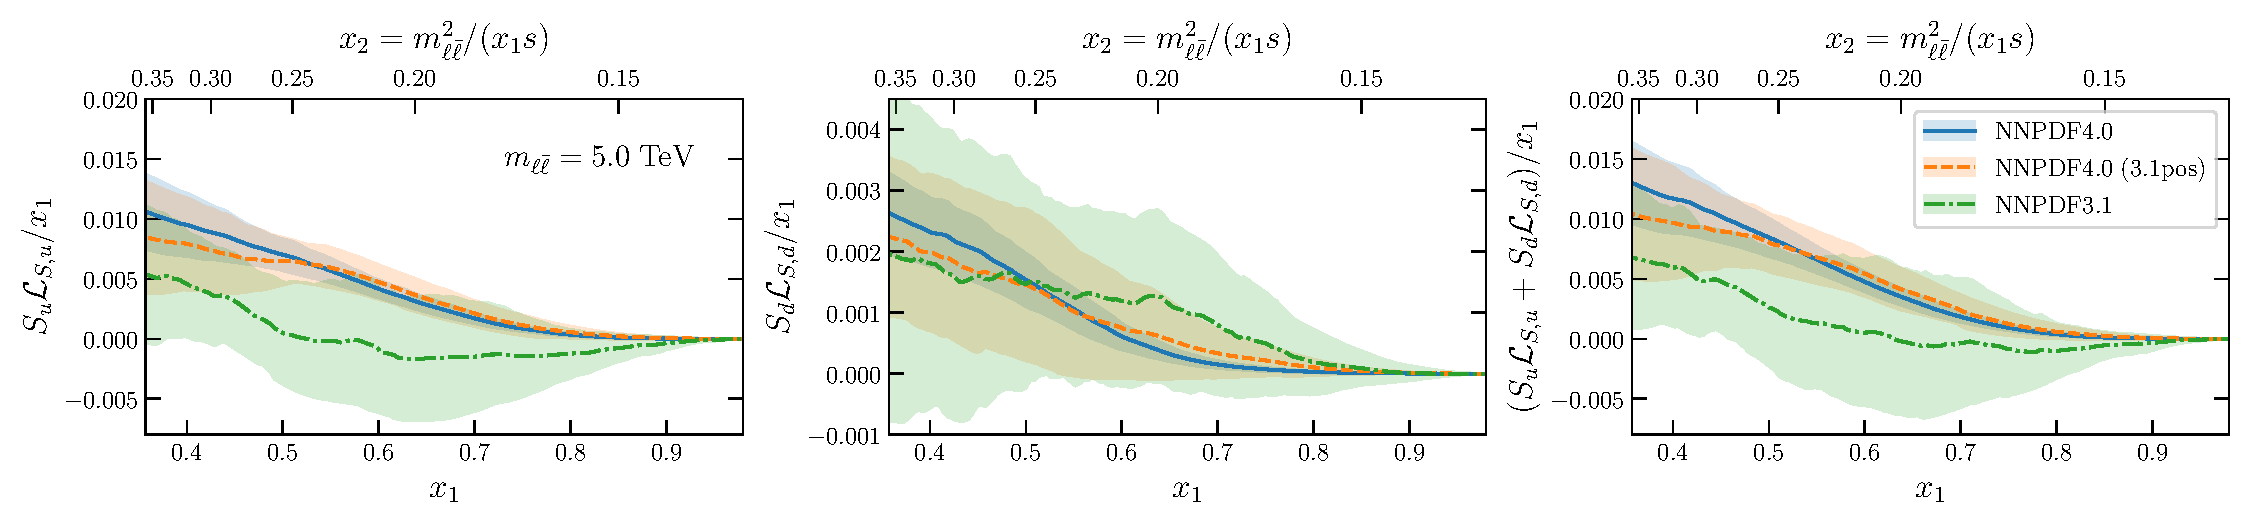
\includegraphics[width=0.99\linewidth]{ch-afb/pdfplot-abs-jacobian-DYlumis-pdfsets-plus-q5p0tev-nnpdf31.pdf}
 \caption{Same as Fig.~\ref{fig:mll_dep_lumi_plus} (upper panels) comparing
\nnpdfr{4.0}, \nnpdfr{4.0}(3.1pos), and NNPDF3.1.
 }    
 \label{fig:pdfplot-absDYlumis-pdfsets-plus-q5tev-nnpdf31}
\end{figure}
%---------------------------------------------------------------------------

The antisymmetric luminosities $\mathcal{L}_{A,q}$, relevant for the
forward-backward asymmetry, are displayed in Fig.~\ref{fig:pdfplot-absDYlumis-pdfsets-minus-q5tev-nnpdf31}
for $\mll = 3$ and 5 TeV respectively.
%
Their qualitative behavior is similar for all  \pdf sets,
with a marked decrease of \pdf uncertainties first from NNPDF3.1
to  \nnpdfr{4.0}(3.1pos)  then
to \nnpdfr{4.0}.
%
Specifically, the qualitative $\mll$ dependence
of $\mathcal{L}_{A,q}$ remains unchanged. Namely, the positive $A_{\rm fb}$
found for $\mll= 3$ TeV decreases 
as the dilepton invariant mass is increased.
%
Hence also for the component of the Drell-Yan cross-section which is odd
in $\cos\theta^*$ we expect \lhc predictions based on NNPDF3.1 to be consistent
with those obtained from \nnpdfr{4.0}.

%-------------------------------------------------------------------------------
\begin{figure}[!t]
 \centering
 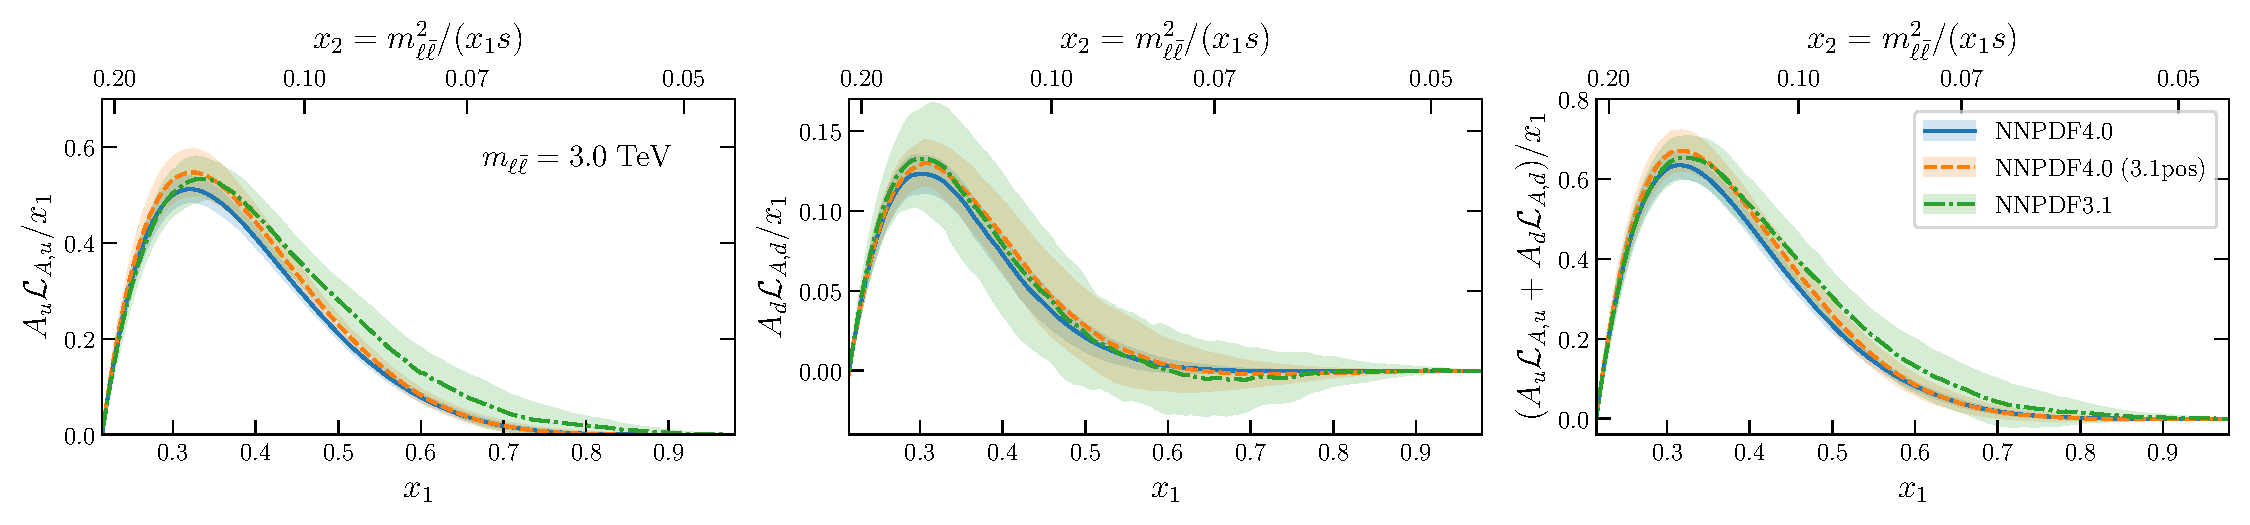
\includegraphics[width=0.99\linewidth]{ch-afb/pdfplot-abs-jacobian-DYlumis-pdfsets-minus-q3p0tev-nnpdf31.pdf}
 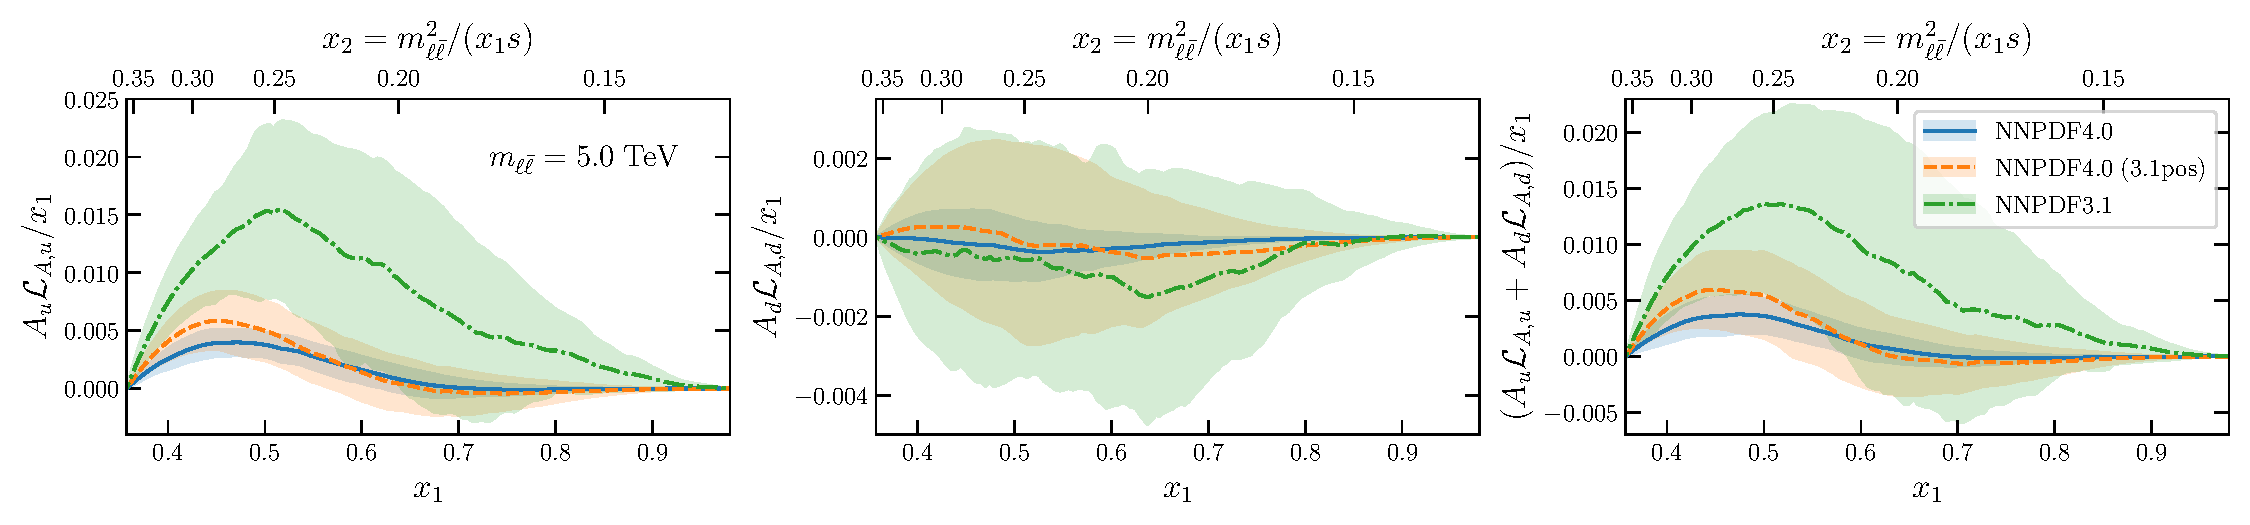
\includegraphics[width=0.99\linewidth]{ch-afb/pdfplot-abs-jacobian-DYlumis-pdfsets-minus-q5p0tev-nnpdf31.pdf}
 \caption{Same as Fig.~\ref{fig:mll_dep_lumi_minus} for the antisymmetric partonic luminosities $\mathcal{L}_{A,q}$,
   comparing \nnpdfr{4.0}, \nnpdfr{4.0}(3.1pos), and NNPDF3.1.
 }    
 \label{fig:pdfplot-absDYlumis-pdfsets-minus-q5tev-nnpdf31}
\end{figure}
%---------------------------------------------------------------------------

These expectations are confirmed by
Fig.~\ref{fig:CMS_DY_14TEV_COSTH_5000_YLL40-vs-31}, which shows the
dilepton rapidity $|y_{\ell\bar{\ell}}|$ 
and the Collins-Soper angle $\cos\theta^*$ distributions for neutral-current DY production
at the \lhc 14 TeV for dilepton invariant masses of $m_{\ell\bar{\ell}}\ge 5$ TeV,
comparing the baseline \nnpdfr{4.0} predictions with those from NNPDF3.1
and \nnpdfr{4.0}(3.1pos).
%
Indeed, 
good agreement within the three \pdf sets is observed with a significant reduction
of \pdf uncertainties between NNPDF3.1 and \nnpdfr{4.0}, consistent
with the behaviour exhibited by the corresponding partonic luminosities.

%-------------------------------------------------------------------------------
\begin{figure}[!t]
 \centering
 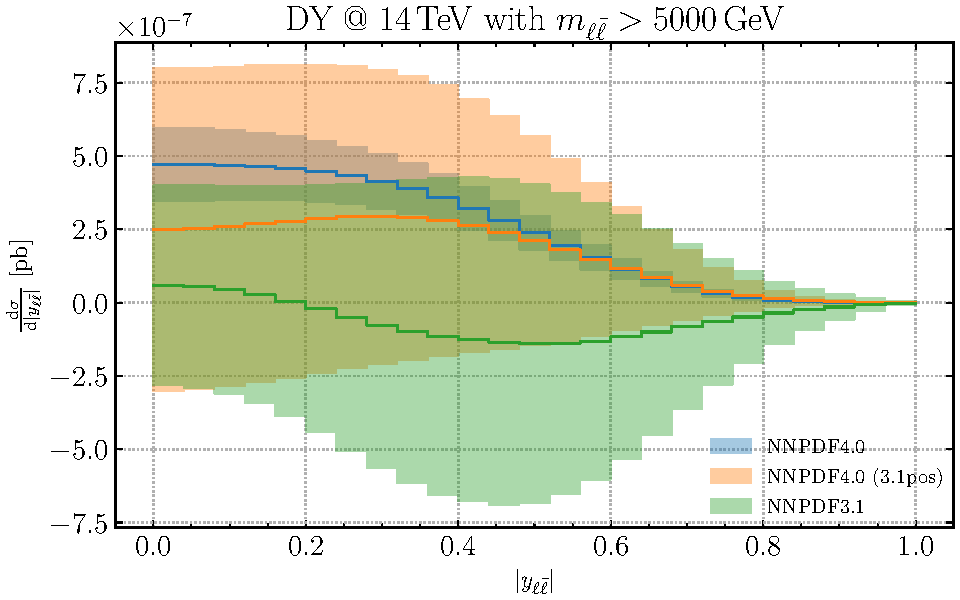
\includegraphics[width=0.49\linewidth]{ch-afb/NNPDF_DY_14TEV_BSM_AFB_YLL_5000-40-vs-31}
 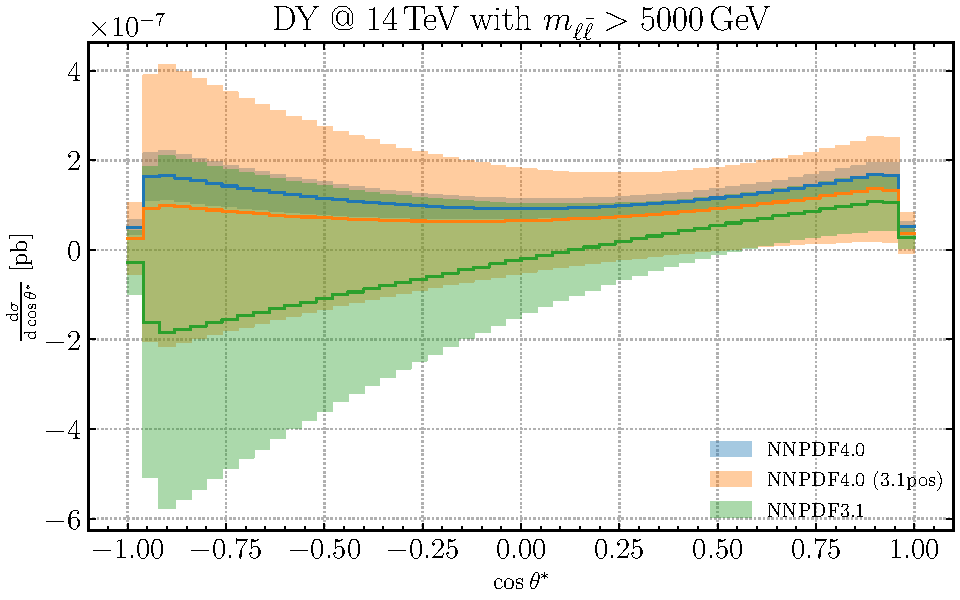
\includegraphics[width=0.49\linewidth]{ch-afb/NNPDF_DY_14TEV_BSM_AFB_COS_5000-40-vs-31}
 \caption{Same as Figs.~\ref{fig:CMS_DY_14TEV_MLL_5000_rap}
and~\ref{fig:CMS_DY_14TEV_MLL_others}
for the absolute dilepton rapidity $|y_{\ell\bar{\ell}}|$ (left)
and the $\cos \theta^*$  (right) distributions
for dilepton invariant masses of $m_{\ell\bar{\ell}}\ge 5$ TeV
 comparing
\nnpdfr{4.0}, \nnpdfr{4.0}(3.1pos), and NNPDF3.1.
 }    
 \label{fig:CMS_DY_14TEV_COSTH_5000_YLL40-vs-31}
\end{figure}
%---------------------------------------------------------------------------


    % !TeX root = ../../../main.tex

%************************************************
\chapter{Forward-Backward Asymmetry}
\label{ch:afb}
%************************************************
\minitoc
\adjustmtc


% !TeX root = ../../../main.tex

The first fundamental application of the integrated pineline will actually the
inclusion of \acrfull{mhou} at \nnlo in the \nnpdfr{4.0} fit.

\pdfs are non-perturbative objects, so it may seem counter-intuitive that their
accuracy depends on perturbative series truncation.
%
This is a direct consequence of extracting them from high energy collisions
data: they are completely determined by physics that happens in the
perturbative regime, and the map discussed at the beginning of this chapter
(the one that connects data to \pdfs) is completely determined by \pqft
calculations.
%
So, the origin of the perturbative order of \pdf sets is exactly determined by
the theory predictions used during the extraction: a \nnlo set is a \pdf set
that has been fitted using theory predictions at \nnlo.
%
A \pdf set directly computed with non-perturbative methods would have no
perturbative order associated, even when used in a perturbative calculation
\footnote{
	From that point of view would be an \textit{all-order} object, even though
	it might be subject to other kinds of approximations.
}\footnote{
	Also consider that \dglap evolution is perturbative, so, once evolved, it
	acquires again a dependency on the perturbative truncation.
}.

The perturbative series enters in the \pdf in two different places: the
partonic cross section calculations (those encoded in \textit{grids}) and the
\dglap evolution\footnote{
	That technically is used twice: during the fit, to bridge data with the
	boundary condition candidate, and to evolve the final boundary condition to
	all scales.
	But considering the \pdf a function of two variables ($z$ and $\mu_F^2$)
	consistently, the abstract evolution flow used is a single one.
}.
%
In principle, these are two different perturbative orders, thus there is not a
single truncation, but two of them, and they can happen at two different
orders.
%
Still, the two objects are not completely decoupled: \dglap evolution arise
from collinear divergences, subtracted by the chosen factorization scheme.
These collinear logarithms appear as well in the partonic cross sections, so it
is important to properly account for them, avoiding double counting.
%
The whole picture of collinear subtractions is deeply connected to treatment of
quark masses, better discussed in \cref{ch:dis}, since a finite value of the
mass regulates the collinear divergence on its own.
%
Therefore, the double perturbative order already appears in the partonic cross
sections calculations, where the \fns chosen can account for light and heavy
quarks at two distinct orders (cf. \cite{Forte:2010ta}, in particular the
FONLL-B scheme).


\section{Anatomy of Drell-Yan production}
\label{sec:afb/HMDY}
% !TeX root = ../../../main.tex

The aim of this  section is to scrutinize the \pdf dependence of the
neutral-current \acrlong{dy} differential cross-section and of the associated
forward-backward asymmetry by reviewing the \lo kinematics, determining \lo
analytic expressions, and finally comparing these analytical calculations to
the results of \lo and \nlo  numerical simulations obtained using \mgamc,
\cite{Alwall:2014hca}, interfaced to \pineappl,
\cite{Carrazza:2020gss,christopher_schwan_2022_7023438}.
%
Specifically, we will relate the behavior of the differential distribution and
asymmetry to the relevant parton luminosities.

\subsection{Drell-Yan kinematics and cross-sections at \lo}
\label{sec:dylo}

We consider dilepton production via the exchange of an electroweak neutral
gauge boson $Z/\gamma^*$ in proton-proton collisions:
\begin{equation}
  \label{eq:DYprocess}
  \mathrm{p}(k_1) + \mathrm{p}(k_2) \to Z/\gamma^*(q) \to \ell(p_{\ell}) + \bar{\ell}(p_{\bar{\ell}}) + X \text{.}
\end{equation}
The hadronic differential cross-section $\dd\sigma^{\mathrm{p}\mathrm{p}\to\llb}$  is factorized in
terms of \pdfs $f_i$ and the partonic cross sections
$\dd\hat\sigma_{ij}$ for incoming partons of species $i,\,j$ as
\begin{equation}
  \dd\sigma^{\mathrm{p}\mathrm{p}\to\llb} = \sum_{ij} \int\limits_0^1\!\dd x_1 \dd
  x_2 f_i(x_1,\mu_F^2) f_j(x_2,\mu_F^2) \dd\hat\sigma_{ij}(\hat k_1 = x_1
  k_1, \hat k_2 = x_2 k_2).
  \label{eq:factorization}
\end{equation}
In the sequel we will set the  factorization scale $\mu_F$ to the
invariant mass of the gauge boson, i.e.\ the dilepton
invariant mass, so $\mu^2_F = \mll^2=(p_\ell + p_{\bar{\ell}})^2$.
%
The kinematics and Feynman diagram of the \lo partonic process
in the quark-antiquark channel are shown in \cref{fig:lo-dy}.
We do not consider photon-initiated processes, as they do not affect
the qualitative features of our discussion.

%--------------------------------------
\begin{figure}[t]
  \centering

  \begin{tikzpicture}
    \begin{feynman}
      \tikzfeynmanset{large}

      \vertex (b);
      \vertex [above left=of b] (a) {\(q\)};
      \vertex [below left=of b] (f1) {\(\bar{q}\)};
      \vertex [right=of b] (c);
      \vertex [above right=of c] (f2) {\(\ell\)};
      \vertex [below right=of c] (f3) {\(\bar{\ell}\)};

      \diagram* {
      (a) -- [fermion, momentum=\(\hat{k}_1\)] (b) -- [fermion, rmomentum=\(\hat{k}_2\)] (f1),
      (b) -- [boson, edge label'=\(\gamma / Z\), momentum=\(q\)] (c),
      (c) -- [anti fermion, momentum=\(p_{\ell}\)] (f2),
      (c) -- [fermion, momentum=\(p_{\bar{\ell}}\)] (f3),
      };
    \end{feynman}
  \end{tikzpicture}

  \caption{Neutral-current Drell-Yan production at \lo in the quark-antiquark channel.}
  \label{fig:afb/lo-dy}
\end{figure}

%--------------------------------------

At \lo, the momentum fractions of the two incoming partons are fully
fixed by knowledge of the invariant mass and rapidity of the gauge
boson, i.e.\ of the dilepton pair  $\yll = (y_\ell + y_{\bar{\ell}})/2$: 
\begin{equation}
  \label{eq:x_fractions}
  x_1 = \frac{ \mll}{\sqrt{s}}\exp(\yll) \, ,\quad x_2 = \frac{
  \mll}{\sqrt{s}}\exp(-\yll) \, ,
\end{equation}
where the center of mass energy of the hadronic collision is
$s=(k_1+k_2)^2$ and at \lo
$\mll^2 = \hat s = x_1 x_2 s$. The absolute dilepton
rapidity thus lies in the range $|\yll|\le \ln (\sqrt{s}/\mll)$.
Beyond \lo there might be extra radiation in the final state, so the \lo
kinematics provides a lower bound on the momentum fractions of the
incoming partons, and all values of the momentum
fractions such that $x_{1,2}\ge \mll/\sqrt s$ are allowed.

It is useful to define the so-called  Collins-Soper
angle $\theta^*$~\cite{Collins:1977iv}, which in the hadronic \acrfull{com}
frame is defined as
\begin{equation}
\begin{split}
  \cos\theta^* &= \sign (\yll) \cos\theta \, ,\\
  \cos\theta &\equiv\frac{p_\ell^+ p_{\bar{\ell}}^- - p_\ell^- p_{\bar{\ell}}^+}{\mll \sqrt{\mll^2 + p_{\mathrm{T},\ell\bar{\ell}}^2}} \text{,} \quad p^\pm = p^0 \pm p^3 \text{.}
  \label{eq:cosine-cs-angle}
\end{split}
\end{equation}
It is easy to show that the Collins-Soper angle $\theta^*$ coincides with the
scattering angle of the lepton in the partonic \com frame, $\bar\theta$.
%
The latter is defined in terms of the lepton momentum as 
\begin{equation}
 \cos\bar\theta \equiv \frac{p^z_\ell}{\mll} \,, \label{eq:coscm}
\end{equation}
where the $z$ axis is along the direction of the incoming quark-antiquark pair.
%
In the partonic \com frame, of course, $p^z_\ell=-p^z_{\bar \ell}$ and $\yll
=0$, so
\begin{equation}
p^\pm_\ell=p^{\mp}_{\bar{\ell}}=  \mll \left( 1\pm \cos{\bar\theta} \right)\, ,
\end{equation}
and substituting in \cref{eq:cosine-cs-angle} it immediately follows that,
taking the convention 
$\sign (\yll)=\sign(0)=+1$, 
$\cos\theta^*=\cos\theta=\cos{\bar\theta}$.
%
The expression of $\cos\theta$ in \cref{eq:cosine-cs-angle} is manifestly
invariant upon boosts along the $z$ axis, so the identification of $\theta$
with the \com scattering angle $\bar\theta$ remains true in any reference
frame.

Note that the definition \cref{eq:coscm} requires a choice for the positive
direction of the $z$ axis, which is usually taken along the direction of the
incoming fermion (quark).
%
This direction is  not experimentally accessible in proton-proton collisions,
so the Collins-Soper angle is defined by always taking the positive $z$ axis in
the direction of the boosted dilepton pair, i.e., at \lo, along the direction of
the incoming quark with largest momentum fraction, i.e.\ by supplementing in
the definition a factor $\sign(\yll)$.
%
Hence $\cos\theta^*=\cos{\bar\theta}$ ($\cos\theta^*=-\cos{\bar\theta}$)  if
the momentum fraction of the incoming quark (antiquark) is the largest.

%
The hard scattering matrix elements that enter the partonic cross-section
in \cref{eq:factorization} are the sum of a pure photon-exchange
contribution, a photon-$Z$ interference term, and a pure $Z$-exchange
contribution.
%
Of course, in the region
$\mll \gtrsim m_Z$ these contributions are all of the same order.
%
Standard arguments~\cite{Peskin:1995ev} then imply that, because in the
Standard Model the photon
coupling to leptons is vector  while the $Z$ coupling is chiral,
the pure photon and pure $Z$ contributions to the cross-section are
necessarily  even in $\cos\theta^*$ while the interference term is
odd.

Specifically, at \lo the fully differential hadronic cross-section can
be obtained from the well-known result~\cite{Peskin:1995ev} for
$e^+e^-\to\mu^+\mu^-$ by replacing the incoming lepton charges  with
those of the quarks, and accounting for the \pdfs, with
the result
\begin{align}
    \frac{\dd^3 \sigma}{\dd \mll \, \dd \yll \, \dd\cos\theta^*} &= \frac{\pi \alpha^2}{3 \mll s} \left((1+\cos^2({\theta^*})) \sum_q S_q \left[f_q(x_1,\mll^2) f_{\bar{q}}(x_2,\mll^2) + f_q(x_2,\mll^2) f_{\bar{q}}(x_1,\mll^2) \right] \right. \nonumber\\
    &\hspace*{15pt} + \left. \cos\theta^* \sum_q A_q \sign (\yll) \left[ f_q(x_1,\mll^2) f_{\bar{q}}(x_2,\mll^2) - f_q(x_2,\mll^2) f_{\bar{q}}(x_1,\mll^2)\right] \right) \, ,
    \label{eq:lo-triple-diff}
\end{align}
where  $\alpha$ is the QED coupling and the even (symmetric) and
odd  (antisymmetric) couplings are given by
\begin{align}
  \label{eq:coup}
    S_q &= e_l^2 e_q^2 + P_{\gamma Z} \cdot  e_l v_l e_q v_q + P_{ZZ} \cdot  (v_l^2+a_l^2)(v_q^2+a_q^2) \nonumber \\
    A_q &= P_{\gamma Z} \cdot 2 e_l a_l e_q a_q  + P_{ZZ} \cdot 8 v_l a_l  v_q a_q \, ,
\end{align}
in terms of the electric charges  $e_l$, $e_q$ and the vector and
axial couplings $v_l$, $v_q$ and $a_l$, $a_q$  of the leptons and
quarks, and the propagator factors
\begin{align}\label{eq:propgz}
    P_{\gamma Z}(\mll) &= \frac{2\mll^2 (\mll^2  - m_Z^2)}{\sin^2(\theta_W) \cos^2(\theta_W)\left[(\mll^2 - m_Z^2)^2 + \Gamma_Z^2 m_Z^2\right]}\\
\label{eq:propzz}
    P_{ZZ}(\mll) &= \frac{\mll^4}{\sin^4(\theta_W) \cos^4(\theta_W)\left[(\mll^2 - m_Z^2)^2 + \Gamma_Z^2 m_Z^2\right]},
\end{align}
with $m_Z$  and $\Gamma_Z$ respectively the $Z$ mass and width and $\theta_W$ the weak mixing angle.
%
In \cref{fig:lo-couplings} we display the
symmetric $S_q$ (left) and antisymmetric $A_q$ (right)
couplings, \cref{eq:coup}, for up-like and
down-like quarks, as a function of 
the dilepton invariant mass $\mll$.
%
Both couplings are around a factor 2 larger for
up-like quarks than for down-like quarks, and
become $\mll$-independent for $\mll \gsim 1$ TeV, where they take
the asymptotic values $\bar S_q$, $\bar A_q$ obtained by
substituting in \cref{eq:coup} the large-mass expressions of
the propagator factors
\begin{equation}\label{eq:propasympt}
    \bar P_{\gamma Z} = \frac{2}{\sin^2(\theta_W)\cos^2(\theta_W)},
    \qquad 
    \bar P_{ZZ} = \frac{1}{\sin^4(\theta_W) \cos^4(\theta_W)},
\end{equation}
to which $P_{\gamma Z}$ and $P_{ZZ}$ respectively reduce up to $O(m^2_Z/\mll^2)$ corrections.

 
%%%%%%%%%%%%%%%%%%%%%%%%%%%%%%%%%%%%%%%%%%%%%%%%%%%%
\begin{figure}
  \centering
  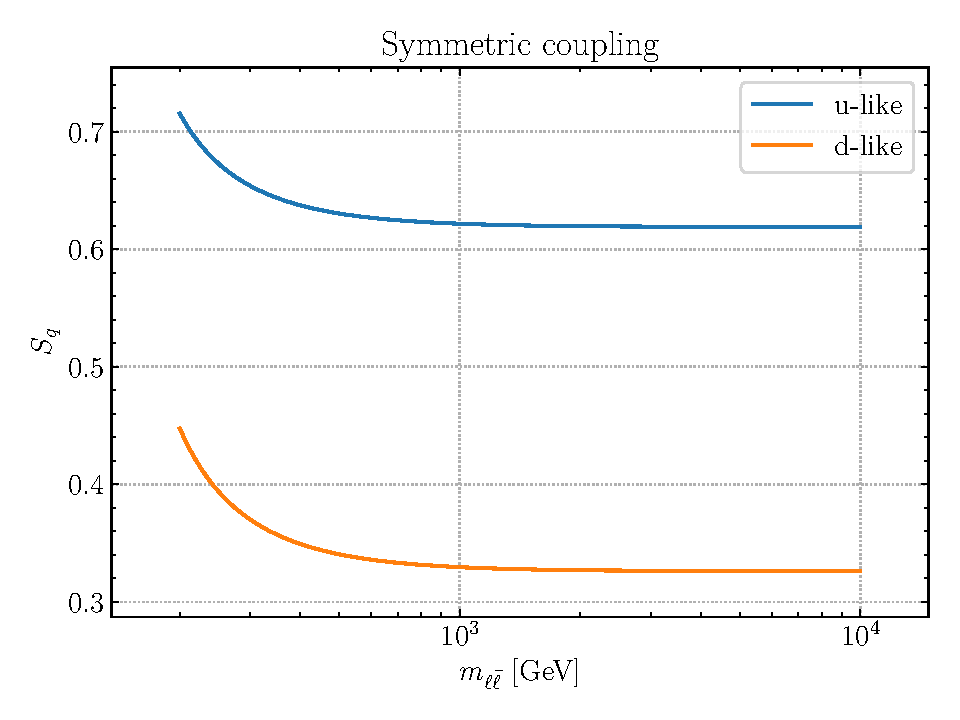
\includegraphics[width=0.49\linewidth]{ch-afb/symmetric-couplings.pdf}
  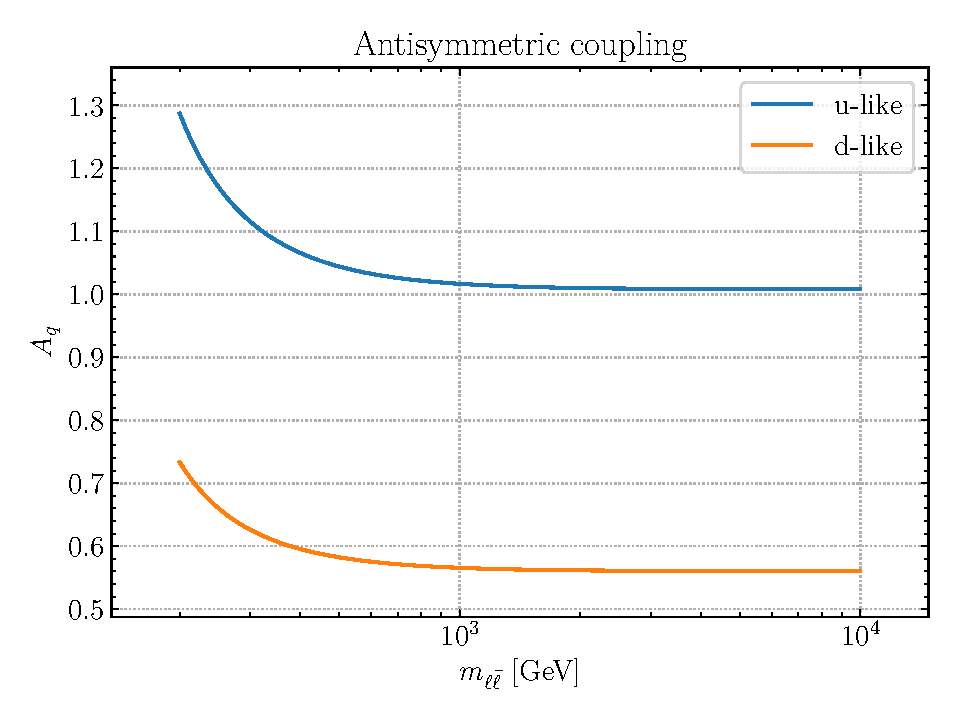
\includegraphics[width=0.49\linewidth]{ch-afb/antisymmetric-couplings.pdf}
  \caption{The symmetric $S_q$ (left) and antisymmetric $A_q$ (right)
    couplings, \cref{eq:coup}, for up-like and
    down-like quarks, as a function of 
 the dilepton invariant mass $\mll$.
  }
  \label{fig:lo-couplings}
\end{figure}
%%%%%%%%%%%%$$$$$$$$$$$$$$$$$$$$$%%%%%%%%%%%%%

The interference term proportional to
$A_q$ is odd in the Collins-Soper angle $\cos\theta^*$, leading to a forward-backward
scattering asymmetry.
%
In a proton-proton collision the initial state is completely
symmetric, so the quark and antiquark contributions to the
cross-section \cref{eq:lo-triple-diff} are necessarily symmetric
upon the interchange of the incoming quark and antiquark, with the
corresponding momentum fractions fixed at \lo by
\cref{eq:x_fractions}.
%
However, as mentioned, there
is a sign change in the relation between $\cos\theta^*$ and
$\cos\theta$ according to whether the incoming parton with largest
momentum fraction is a quark or an antiquark, i.e.,
when interchanging
$x_1$ with $x_2$ in the argument of the quark and antiquark \pdfs,
thereby leading to the result of  \cref{eq:lo-triple-diff}.
%
This leads
to a forward-backward asymmetry whenever the quark and antiquark
\pdfs have different $x$ dependence.

In order to understand the relation of this forward-backward
asymmetry in terms of the
behavior of the \pdfs, it is convenient
to rewrite the \pdf combinations that contribute to the differential
cross-section \cref{eq:lo-triple-diff} in terms of symmetric and
antisymmetric parton luminosities, defined as
\begin{align}
  \mathcal{L}_{S,q}(\mll, \yll) &\equiv f_q(x_1,\mll^2) f_{\bar{q}}(x_2,\mll^2) + f_q(x_2,\mll^2) f_{\bar{q}}(x_1,\mll^2) \, ,
  \nonumber\\
  \mathcal{L}_{A,q}(\mll, \yll) &\equiv \sign (\yll) \left[ f_q(x_1,\mll^2) f_{\bar{q}}(x_2,\mll^2) - f_q(x_2,\mll^2) f_{\bar{q}}(x_1,\mll^2)\right] \, , \label{eq:symm_asymm_lumis}
\end{align}
where the momentum fractions $x_1$ and $x_2$ are given in terms of $\mll$, $\yll$,
and $\sqrt{s}$ in \cref{eq:x_fractions}.
Note that both parton luminosities are invariant under
the interchange $x_1\leftrightarrow x_2$, upon which $\yll \to -\yll$.
%
In terms of these luminosities, the triple differential cross-section \cref{eq:lo-triple-diff}
takes the compact form
\begin{equation}
  \label{eq:lo-triple-diff-lumis}
  \frac{\dd^3 \sigma}{\dd \mll \, \dd \yll \, \dd\cos\theta^*} =
  \frac{\pi \alpha^2}{3 \mll s} \left( (1+\cos^2({\theta^*})) \sum_q S_q \mathcal{L}_{S,q}(\mll, \yll)
  + \cos\theta^* \sum_q A_q \mathcal{L}_{A,q}(\mll, \yll)  \right) \, ,
\end{equation}
which explicitly displays
its symmetry properties upon the transformation $\cos\theta^* \to -\cos\theta^*$,
equivalent to a charge conjugation transformation 
$q\leftrightarrow \bar q$ and $\ell \leftrightarrow \bar{\ell} $.

The symmetric and antisymmetric parton luminosities \cref{eq:symm_asymm_lumis} can also be expressed
in terms of the sum and difference of quark and antiquark \pdfs,
\begin{equation}
  \label{eq:fqpm}
  f_{q}^\pm \left( x, Q\right) = f_{q} \left( x, Q\right) \pm f_{\bar{q}} \left( x, Q\right) \, ,
\end{equation}
where $f_{q}^-$ is usually called the valence \pdf combination, and $f_{q}^+$
the total quark \pdf\@. Note that at \lo, and more generally in factorization
schemes in which \pdfs are positive, such as $\mmsbar$ \cite{Candido:2020yat},
$f^+_q$ is positive while $f_q^-$ in general is not, and $f_{q}^+>|f_{q}^-|$.
%
We can write the symmetric and antisymmetric parton luminosities in
\cref{eq:symm_asymm_lumis} as
\begin{align}
  \mathcal{L}_{S,q}(\mll, \yll) &= \frac {1} 2 \left( f_q^+(x_1,\mll^2) f_{q}^+(x_2,\mll^2) - f_q^-(x_2,\mll^2) f_{q}^-(x_1,\mll^2)  \right) \, \label{eq:lumiss_qpm}\\
  \mathcal{L}_{A,q}(\mll, \yll) &= \frac {\sign (\yll)} 2 \left( f_q^-(x_1,\mll^2) f_{q}^+(x_2,\mll^2) - f_q^-(x_2,\mll^2) f_{q}^+(x_1,\mll^2)  \, \right) \,. \label{eq:lumisa_qpm}
\end{align}

The symmetric luminosity $\mathcal{L}_{S,q}$ is of course positive, and it is
dominated by the $f_q^+(x_1,\mll^2) f_{q}^+(x_2,\mll^2)$ term, which is always
larger than the valence contribution  $f_q^-(x_2,\mll^2) f_{q}^-(x_1,\mll^2)$.
The sign of the antisymmetric combination, that in turn drives the sign of the
forward-backward asymmetry, is in general not determined uniquely.
%
If $x_1$ is in the region of the valence peak, and $x_2$ in the small $x$
region, then $f^-(x_1,\mll^2)\gg f^-(x_2,\mll^2)$, and the antisymmetric
luminosity is positive provided only that the valence \pdf is positive.
%
As we will discuss in Sect.~\ref{sec:largexpdfs},
while this is indeed the case in
the $Z$-peak region, it is actually not necessarily the case in the
high dilepton mass region relevant for \bsm searches.

\subsection{Single-differential distributions and the forward-backward asymmetry}
\label{sec:numlo}
Starting from the triple differential cross section,
\cref{eq:lo-triple-diff-lumis}, one can define 
single differential distributions by integrating the other two kinematic variables
over the available phase space.
%
In particular, the single-differential distribution in the
Collins-Soper angle $\theta^*$ is given by
\begin{equation}
  \label{eq:dsigma-dcos}
  \frac{\dd\sigma}{\dd\cos\theta^*} = \int\limits_{\mll^{\text{min}}}^{\sqrt s}\!\dd\mll\!\!\int\limits_{\ln(\mll/\sqrt s)}^{\ln(\sqrt s/\mll)}\!\!\dd\yll\, \frac{\dd^3 \sigma}{\dd \mll \, \dd \yll \, \dd\cos\theta^*} \, ,
\end{equation}
where $\mll^{\text{min}}$ is a lower kinematic cut in the dilepton invariant mass.
%
Since \cref{eq:lo-triple-diff-lumis} falls off steeply with $\mll$, the region
with $\mll \gsim \mll^{\text{min}}$ will dominate the integral.
%
Given that the dependence of the fully differential cross-section
\cref{eq:lo-triple-diff-lumis}
on  the Collins-Soper angle factorizes with respect to the \pdf
dependence, the integration over rapidity and invariant mass does not
affect the  $\cos\theta^*$ dependence, and the single-differential
cross section \cref{eq:dsigma-dcos} takes the simple form 
\begin{equation}
  \label{eq:dsigma-dcos-v2}
  \frac{\dd\sigma}{\dd\cos\theta^*} = (1+\cos^2\theta^*)\sum_q g_{S,q} + \cos\theta^*\sum_q g_{A,q} \, ,
\end{equation}
where the symmetric and antisymmetric coefficients $g_{S,q}$ and $g_{A,q}$ depend on the quark flavor
and on the invariant mass cut $\mll^{\text{min}}$, but not on the
Collins-Soper angle itself.
%
The contributions relevant for the forward-backward asymmetry, $g_{A,q}$,
are given at \lo by
\begin{equation}
\label{eq:gAq_integrated_1}
g_{A,q} =\frac{\pi \alpha^2}{3 s} \int\limits_{\mll^{\text{min}}}^{\sqrt s}\frac{\dd\mll}{\mll}A_{q}(\mll)\!\!\int\limits_{\ln(\mll/\sqrt s)}^{\ln(\sqrt s/\mll)}\!\!\dd\yll\, \mathcal{L}_{A,q}(\mll,\yll) \, ,
\end{equation}
which in the large-$\mll$ region,
 expressing the longitudinal momentum integration in terms of
$x_1$ (assuming $x_1~\ge x_2$), becomes
\begin{equation}
  g_{A,q} = \frac{\pi \alpha^2\bar A_q}{3 s} \int\limits_{\mll^{\text{min}}}^{\sqrt s}\frac{\dd\mll}{\mll}
  \!\!\int\limits_{\mll/\sqrt s}^{1}\!\!\frac{\text{d}x_1}{x_1}\, 
  \mathcal{L}_{A,q}(\mll,x_1)+\mathcal{O} \left(\frac{m_Z^2}{\mll^2}\right) \, ,
  \label{eq:gAq_integrated}
\end{equation}
where the $\mll$-independent effective couplings $\bar A_q$  are
given substituting in \cref{eq:coup} the expressions for
the asymptotic propagator factors \cref{eq:propasympt}.

Upon integration over the Collins-Soper angle, the
antisymmetric contribution vanishes: so for instance the
rapidity distribution
\begin{equation}
  \label{eq:dsigma-dyll}
  \frac{\dd\sigma}{\dd\yll} = \int\limits_{\mll^{\text{min}}}^{\sqrt s}\!\dd\mll \int\limits_{-1}^{1}\!\!\dd\cos\theta^*\, \frac{\dd^3 \sigma}{\dd \mll \, \dd \yll \, \dd\cos\theta^*} \, ,
\end{equation}
does not depend on terms proportional to $A_q$.
%
Hence, for \bsm searches in which one is
interested in the interference terms, as well as for \pdf studies in which one is
interested in the valence-sea separation, the forward-backward
asymmetry is especially relevant.
%
This observable is
defined at the differential level as
\begin{equation}
  A_{\text{fb}}(\cos\theta^*) \equiv \frac{ \frac{\dd\sigma}{\dd\cos\theta^*}(\cos\theta^*)
  - \frac{\dd\sigma}{\dd\cos\theta^*}(-\cos\theta^*)}{ \frac{\dd\sigma}{\dd\cos\theta^*}(\cos\theta^*)
  + \frac{\dd\sigma}{\dd\cos\theta^*}(-\cos\theta^*) } \, ,\quad \cos\theta^*>0 \, ,
  \label{eq:forward-backward-asymmetry}
\end{equation}
which in terms of the coefficients introduced in
\cref{eq:dsigma-dcos-v2} is given at \lo by
\begin{equation}
  \label{eq:afb_lo}
  A_{\text{fb}}(\cos\theta^*)   = \frac{\cos\theta^*}{(1+\cos^2(\theta^*))}\frac{\sum_q g_{A,q} }{\sum_{q'} g_{S,q'}} \, ,\quad \cos\theta^*>0 \,.
\end{equation}
This  shows that the dependence on $\cos\theta^*$ factorizes
and the \pdf dependence only appears as an overall normalization factor
depending on the ratio of $\sum_q g_{A,q}$
and $\sum_q g_{S,q}$, which in turn depend on the antisymmetric and symmetric
partonic luminosities $ \mathcal{L}_{A,q}$ and $ \mathcal{L}_{S,q}$ respectively.
%
Note that the overall sign of $A_{\text{fb}}$ remains in general undetermined.

%%%%%%%%%%%%%%%%%%%%%%%%%%%%%%%%%%%%%%%
\begin{figure}[t]
  \centering
  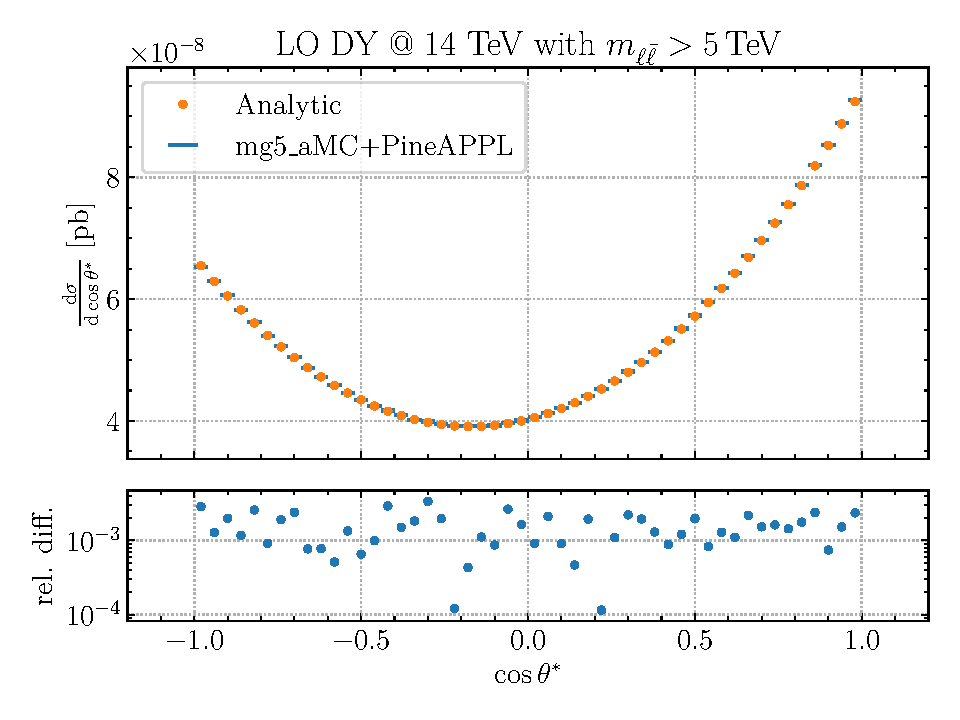
\includegraphics[width=0.49\linewidth]{ch-afb/sigma_grid_ana-MLL_5000_COSTH-r3.pdf}
  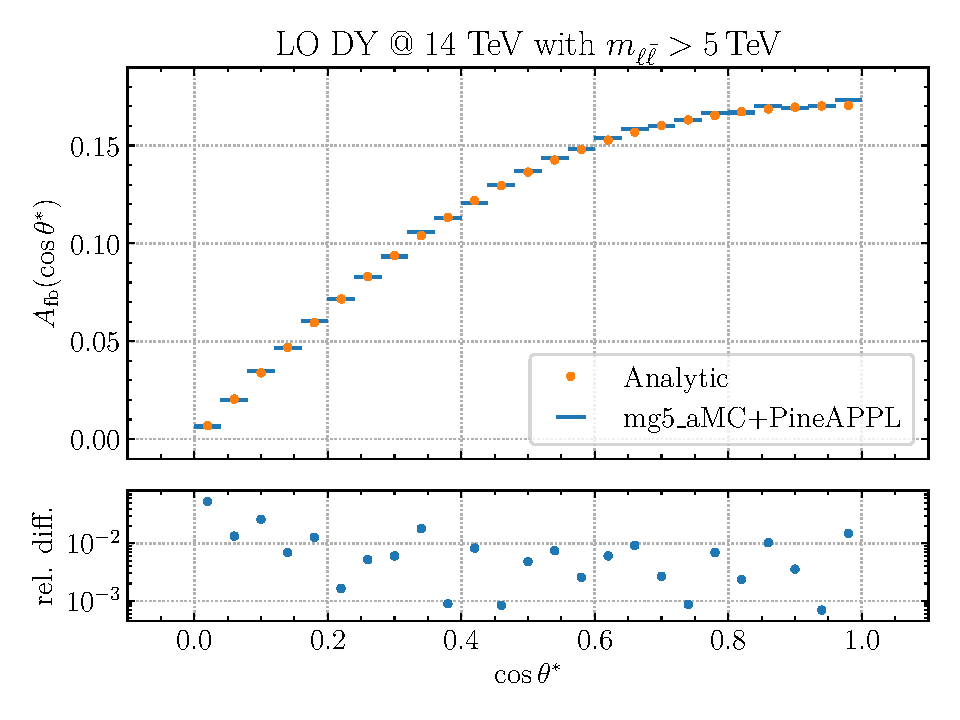
\includegraphics[width=0.49\linewidth]{ch-afb/afb_grid_ana-MLL_5000_COSTH-r3.pdf}
  \caption{The single-inclusive differential distribution in
    the Collins-Soper angle $\cos\theta^*$,
    \cref{eq:dsigma-dcos},
    and the corresponding forward-backward asymmetry computed at \lo,
    where the analytic calculation  \cref{eq:forward-backward-asymmetry}
    is compared with the numerical simulation based on 
    \mgamc
    interfaced to \pineappl.
    %
    The bottom panels display the relative difference between the analytic and
    numerical calculations.
    %
    One of the replicas of the \nnpdfr{4.0} \nnlo \pdf set is used as input
    to the calculation.
  }    
  \label{fig:lo-diff-cos}
\end{figure}
%%%%%%%%%%%%%%%%%%%%%%%%%%%%%%%

In order to illustrate concretely these results,  
in \cref{fig:lo-diff-cos} we display the
single-inclusive differential distribution in $\cos\theta^*$,
\cref{eq:dsigma-dcos},
and the corresponding forward-backward asymmetry,
\cref{eq:forward-backward-asymmetry} evaluated at \lo
for $\mll^{\text{min}}=\SI{5}{\TeV}$. The single-differential rapidity
distribution \cref{eq:dsigma-dyll}) is also shown for reference in Fig.~\ref{fig:lo-diff-yll}.
%
We display both a numerical evaluation based on \mgamc interfaced to \pineappl,
as well as analytic results found using the form \cref{eq:lo-triple-diff-lumis}
of the triple differential luminosity, with all the values of the parameters
entering \crefrange{eq:coup}{eq:propzz} set to the values used in the \mgamc
runcard, and performing  numerically the integrals in
\cref{eq:dsigma-dcos,eq:dsigma-dyll}.
%
For validation purposes, no kinematic cuts are applied to the rapidities and
transverse momenta of final-state leptons.
The \pdf input is taken to be given, for illustrative purposes, by one of the
replicas of the \nnpdfr{4.0} \nnlo set.
The relative difference between the analytic and numerical calculation is shown
in the bottom panels of \cref{fig:lo-diff-cos} and demonstrates perfect
agreement. 

While the discussion so far has been presented  at \lo, its qualitative
features are unaffected by  higher-order corrections.
%
To illustrate this, in \cref{fig:lo-kfact} we compare the \lo result  from
\cref{fig:lo-diff-cos} to the corresponding \nlo \qcd result.
%
The bottom panels display the \nlo $K$-factor for the $\cos\theta^*$
distribution and the forward-backward asymmetry.
%
Whereas the \nlo $K$-factor in the $\cos\theta^*$ distribution is quite large
(around 40\%) it exhibits only a mild dependence on the Collins-Soper angle.
%
For $A_{\text{fb}}$, the $K$-factor is at the 10\% level and essentially
independent of the value of $\cos\theta^*$.

%%%%%%%%%%%%%%%%%%%%%%%%%%%%%%%%%%%%
\begin{figure}[t]
  \centering
  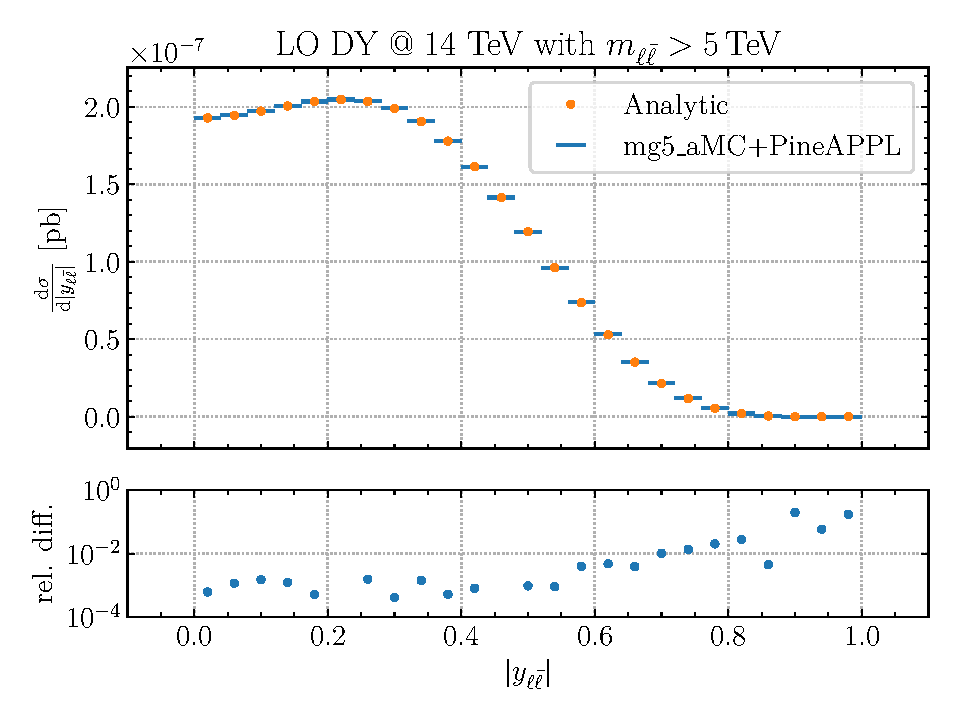
\includegraphics[width=0.49\linewidth]{ch-afb/sigma_grid_ana-MLL_5000_YLL-r3.pdf}
  \caption{Same as \cref{fig:lo-diff-cos} but now for the absolute dilepton rapidity distribution $|\yll|$}
  \label{fig:lo-diff-yll}
\end{figure}
%%%%%%%%%%%%%%%%%%%%%%%%%%%%%%%%%%%%%%%%%%
 
%%%%%%%%%%%%%%%%%%%%%%%%%%
\begin{figure}[t]
  \centering
  \includegraphics[width=0.49\linewidth]{ch-afb/sigma_lo_nlo-MLL_5000_COSTH-r3.pdf}
  \includegraphics[width=0.49\linewidth]{ch-afb/afb_lo_nlo-MLL_5000_COSTH-r3.pdf}
  \caption{Same as \cref{fig:lo-diff-cos} now comparing the \lo result
    to the \nlo \qcd result obtained using \mgamc.
    %
    The $K$-factor is shown in the lower panel.
  }
  \label{fig:lo-kfact}
\end{figure}
%%%%%%%%%%%%%%%%%%%%%%%%%


\section{The forward-backward asymmetry and the large-\texorpdfstring{$x$}{x} \pdfs}
\label{sec:afb/largexpdfs}
% % !TeX root = ../../../main.tex

After our general discussion of the Drell-Yan process,
we now investigate
 proton structure at large-$x$, focusing on its
impact on the forward-backward asymmetry $A_{\rm fb}\lp \cos\theta^*\rp$
at large invariant masses.
%
First, we discuss the dependence of the
qualitative features of the asymmetry,
and specifically its sign, on the behavior of the underlying \pdfs: we
illustrate this in a toy model, and compare results to a simple and 
commonly used approximation.
%
Subsequently,
we study the large-$x$ behavior of the \pdfs from several
recent \pdf sets: we compare \pdfs, luminosities and the \lo asymmetry
$A_{\rm fb}$ as a function of the dilepton invariant mass $\mll$.

\subsection{Qualitative features of \texorpdfstring{$A_{\rm fb}$}{Afb}}
\label{sec:afb_toy}

In order to understand the main qualitative features of  the $\cos\theta^*$
distribution and of the asymmetry $A_{\rm fb}$ and their dependence on the 
properties of the underlying
\pdfs, it is instructive to evaluate predictions based on the
same computational setup adopted in Sect.~\ref{sec:HMDY}, namely
 \lo matrix elements without kinematic cuts, using toy \pdfs as input.
%
We consider toy quark and antiquark \pdf with  the form
\begin{equation}
  \label{eq:toypdf}
  xf_q(x) = A_qx^{-a_q}(1-x)^{b_q} \, , \quad xf_{\bar{q}}(x) = A_{\bar{q}}x^{-a_{\bar{q}}}(1-x)^{b_{\bar{q}}} \, ,
\end{equation}
where $A_q$ and $A_{\bar{q}}$ are  normalization constants, irrelevant
for this discussion.
%
For simplicity we neglect the scale dependence of
the \pdfs.
%
We then compute the single-differential distribution Eq.~(\ref{eq:dsigma-dcos}) and
the asymmetry Eq.~(\ref{eq:forward-backward-asymmetry}) with different assumptions on the
large $x$-behavior of these toy \pdfs, i.e.\ different values of the large-$x$
exponents $b_q$, $b_{\bar{q}}$.

Since the overall normalization does not affect the shape
of the distribution, we set $A_q=A_{\bar{q}}=1$.
%
Furthermore, since we are not interested in the small-$x$ behavior,
we set $a_q=a_{\bar{q}}=1$. 
%
Hence, we consider simple scenarios in which 
\begin{align}\label{eq:toyp}
xf_q^+(x; b_q,b_{\bar{q}}) &= xf_q(x)+xf_{\bar{q}}(x) = x^{-1}\lc (1-x)^{b_q} +(1-x)^{b_{\bar{q}}}  \rc  \,, \\\label{eq:toym}
xf_q^-(x; b_q,b_{\bar{q}}) &= xf_q(x)-xf_{\bar{q}}(x) = x^{-1}\lc (1-x)^{b_q} -(1-x)^{b_{\bar{q}}}  \rc  \,, 
\end{align}
with different choices of the parameters  $b_q$ and $b_{\bar{q}}$.
Specifically, we consider a scenario with $b_q < b_{\bar{q}} $, in particular
$(b_q,b_{\bar{q}})=(3,5)$, which leads to a positive valence combination $xf_q^-$
for all values of $x$;  a  scenario with
$(b_q,b_{\bar{q}})=(3,3)$ so  $xf_q^-$ vanishes identically; and a third scenario
in which the quark \pdfs at large-$x$ fall off more rapidly than the antiquarks,
$(b_q,b_{\bar{q}})=(5,3)$, so the valence combination $xf_q^-$ becomes negative.

%-----------------------------------------------------------------
\begin{figure}[!t]
 \centering
 \includegraphics[width=0.49\linewidth]{ch-afb/sigma_toy-33-53-35.pdf}
 \includegraphics[width=0.49\linewidth]{ch-afb/afb_toy-33-53-35.pdf}
 \caption{The single-inclusive $\cos\theta^*$ distribution
   Eq.~(\ref{eq:dsigma-dcos})  (left)
   and the corresponding forward-backward asymmetry
   (right panel) Eq.~(\ref{eq:forward-backward-asymmetry}) evaluated using 
    the toy \pdfs of Eq.~(\ref{eq:toypdf}).
   %
   No  kinematic cuts are applied except for $\mll^{\rm min}=5$ TeV.
   %
 }    
 \label{fig:sigma_toy}
\end{figure}
%-----------------------------------------------------------------

In \cref{fig:sigma_toy} we display both the $\cos\theta^*$
single-inclusive distribution Eq.~(\ref{eq:dsigma-dcos}) and
the asymmetry Eq.~(\ref{eq:forward-backward-asymmetry}).
%
It is apparent that if the  antiquark \pdfs fall off at large-$x$ faster than
the quarks, i.e.\ when $b_q < b_{\bar{q}}$ the forward-backward
asymmetry is positive, while if the converse is true it is
negative. Of course if the quark and antiquark \pdfs behave in the same
way there is no asymmetry.
%
In this simple model, a negative asymmetry corresponds to a negative
valence distribution, which conflicts with sum rules and appears to be
unphysical. However, the model should be only taken as illustrative of
the large-$x$ behavior: it is of course easy to construct \pdfs that
reproduce this behavior at very large $x$, while leading to a positive
valence \pdf as $x$ decreases, consistent with sum rules. One could then argue that
Brodsky-Farrar counting rules~\cite{Brodsky:1973kr,Brodsky:1974vy}
imply that  $b_q > b_{\bar{q}}$
hence a positive asymmetry is favored.
%
However,
counting rules are supposed to only hold asymptotically, so whether
they apply in any given region of $x$ is a priori unclear.
%
It is easy
to construct generalizations of the model in which the behavior
leading to a negative asymmetry is reproduced at large enough $x$, yet
the valence \pdfs are positive at smaller $x$, and the counting rules
apply in the strict $x\to1$ limit.

In fact, whereas in the toy model a negative asymmetry is
associated with a negative valence
Eq.~(\ref{eq:toym}), the formal condition for a negative asymmetry is
(assuming $x_1>x_2$)
\begin{equation}\label{eq:signas}
   \sign\left[\mathcal{L}_{A,q}\right]=\sign\left[\frac{ f_q^+(x_2)}{
       f_q^+(x_1)}-\frac{
       f_q^-(x_2)}{f_q^-(x_1)}\right]=\sign\left[\frac{ f_q(x_2)}{
       f_q(x_1)}-\frac{f_{\bar{q}}(x_2)}{f_{\bar{q}}(x_1)}\right] \, , \quad x_1>x_2 \,.
\end{equation}
Hence what determines the sign of the antisymmetric luminosity, and thus
of the forward-backward asymmetry, is the relative rate of decrease of
the quark and antiquark, or valence and total quark \pdfs, rather than
their sign. Again, it is easy to construct generalizations of the
toy model in which the condition Eq.~(\ref{eq:signas}) still holds,  yet
the valence \pdf remains positive.

It is interesting to note that a different conclusion is reached using
an approximation to the asymmetry which is quite accurate  in the $Z$
peak region.
%
This approximation however turns out to fail at high
invariant mass.
%
Indeed, the expression Eq.~(\ref{eq:lumisa_qpm}) of the antisymmetric
luminosity in terms of the valence 
and total \pdf combinations $f_q^+$ and $f_q^-$ \pdf combinations
suggests an approximation based on the expectation
that the valence is dominant at large $x$ and the sea is dominant at
small $x$. Assuming $x_1> x_2$, one then expects that
\be
\mathcal{L}_{A,u}(\yll,\mll) \approx\frac {1}{2} f_u^-(x_1,\mll^2)
f_{u}^+(x_2,\mll^2)   \,  \, ,\quad x_1>x_2.
\label{eq:app_asym_lumi_2}
\ee
This is clearly true  in the $Z$-peak region, which  motivates the
suggestion to use the measurement of $A_{\rm fb}$ as a means to
 constrain the valence quark combinations~\cite{Accomando:2019vqt}.

%-------------------------------------------------------------------------------
\begin{figure}[!t]
 \centering
 \includegraphics[width=0.90\linewidth]{ch-afb/pdfplot-abs-DYlumis-minus-validation-lowQ-nnpdf40.pdf}
 \caption{The  antisymmetric partonic luminosity $\mathcal{L}_{A,q}$, Eq.~(\ref{eq:lumisa_qpm}),
for the up and down quarks 
compared to the approximation 
Eq.~(\ref{eq:app_asym_lumi_2}) in the case of \nnpdfr{4.0}
at $\mll=m_Z$ (top)
and $\mll=5$ TeV (bottom panels).
 }    
 \label{fig:pdfplot-abs-DYlumis-minus-validation-lowQ-nnpdf40}
\end{figure}
%---------------------------------------------------------------------------

However, while Eq.~(\ref{eq:app_asym_lumi_2}) provides
a satisfactory approximation in the  $Z$-peak region,
it fails  at larger $\mll$ values. Indeed, for on-shell $Z$
production, with $\sqrt{s}=14$ TeV,
for a dilepton rapidity with $y_{\ell\bar{\ell}}\sim 2.5$, the limit of the
acceptance region
of ATLAS and CMS, the colliding partons have
$x_1=0.09$ and $x_2=6\times 10^{-4}$. So indeed the contribution in
which the valence \pdf is evaluated at the smallest $x$ value is highly suppressed.
%
But for $\mll=5$~TeV, the smallest value of $x_2$, attained when
$x_1=1$, is $x_2=0.35$: so both momentum fractions are large and in fact
to the right of the valence peak.
%
In such case, there 
is no obvious hierarchy between
the different terms that contribute to to antisymmetric
luminosity $\mathcal{L}_{A,q}$.

This is illustrated in
Fig.~\ref{fig:pdfplot-abs-DYlumis-minus-validation-lowQ-nnpdf40},
where we compare the antisymmetric luminosity $\mathcal{L}_{A,q}$
for the up and down quarks 
to the approximation
Eq.~(\ref{eq:app_asym_lumi_2}), evaluated with \nnpdfr{4.0} \nnlo,
in the $Z$-peak region $\mll=m_Z$ 
and at $\mll=5$ TeV.
%
While indeed for $\mll=m_Z$ Eq.~(\ref{eq:app_asym_lumi_2}) reproduces
the exact luminosity, this is not the case for $\mll\gg m_Z$: both
the magnitude and the shape of the luminosity are  very different.
%
This qualitative behavior is common to all \pdf sets: the approximation
fails equally badly regardless of the \pdf set.

We conclude that there
is no simple relation between the sign of the asymmetry and that of
the valence \pdf, and that the
behavior of the asymmetry must be determined by studying the large-$x$
behavior of the quark and antiquark \pdfs.

\subsection{Parton distributions}
\label{sec:subsec-largexPDFs}

We assess now the large-$x$ behavior of
the quark and antiquark \pdfs in different recent \pdf
determinations: specifically, we compare
 ABMP16,
 CT18,  \nnpdfr{4.0},
 and MSHT20.
%
 For
completeness, in App.~\ref{app:nnpdf31} we also present results
obtained with the widely used NNPDF3.1~\cite{Ball:2017nwa} set.

%-------------------------------------------------------------------------------
\begin{figure}[!t]
 \centering
 \includegraphics[width=1.0\linewidth]{ch-afb/pdfplot-abslargex-nnpdf40.pdf}
 \includegraphics[width=1.0\linewidth]{ch-afb/pdfplot-abslargex-nnpdf40-valence.pdf}
 \caption{\small Comparison of the $xf^+_q$ (top) and $xf_q^-$ (bottom) quark
   \pdf combinations for the up, down, strange, and charm quarks,
   evaluated at $\mll=5$~TeV for \nnpdfr{4.0} \nnlo.
   %
   The right panels display the relative 68\% CL uncertainties.
   %
   The two vertical lines indicate $x_{\rm min}=\mll^2/s$, the
   smallest allowed value of $x$ 
   for dilepton DY production for a collider
   CoM energy $\sqrt{s}=14$~TeV, and the value of $x$
   corresponding to a symmetric partonic collision $x_1=x_2$, namely
 $x_{\rm  sym}=\mll/\sqrt{s}$.
 }    
 \label{fig:pdfplot-abslargex}
\end{figure}
%-------------------------------------------------------------------------------

First, we provide a qualitative assessment of the relative size of the
\pdfs corresponding to
individual quark flavors, both for the total and valence \pdfs.
In Fig.~\ref{fig:pdfplot-abslargex} we
compare  the total $xf^+_q$ and valence $xf_q^-$  quark
   \pdf combinations for the up, down, strange, and charm quarks,
   evaluated at $\mll=5$~TeV with the \nnpdfr{4.0} \nnlo \pdf set.
   %
   The right panels display the corresponding relative 68\% CL uncertainties.
   %
  The leftmost vertical line indicates $x_{\rm min}=\mll^2/s$, the
  smallest allowed value of $x$ 
   for dilepton DY production with invariant mass $\mll=5$~TeV for a collider
   CoM energy $\sqrt{s}=14$~TeV.
   %
   The rightmost vertical line corresponds to
   the value of $x$ in a symmetric partonic collision where $x_1=x_2$, namely
   $x_{\rm  sym}\equiv\mll/\sqrt{s}$.

   From Fig.~\ref{fig:pdfplot-abslargex} one can observe that for
   $x\lesssim 0.3$ there is a clear hierarchy
$f_u^+>f_d^+ >f_s^+>f_c^+$, while for larger $x$ values the
   strange and charm \pdfs become of comparable magnitude.
   %
   The up and down quarks, both for $xf^+_q$ and $xf^-_q$, are significantly larger
   than the second-generation quark \pdfs until $x\simeq 0.7$, and hence dominate the
   large-$\mll$ differential distributions in Drell-Yan production.
%
\pdf uncertainties grow rapidly with $x$, reflecting the lack
of direct experimental constraints.
%
The same qualitative behavior of the lighter versus heavier flavor \pdfs
is observed for other \pdf sets.
%
Given the hierarchy $f_u^\pm, f_d^\pm \gg f_s^\pm, f_c^\pm $, in the following
we will discuss only the behavior of the first-generation quark
and antiquark \pdfs which are those relevant for the interpretation
of neutral-current Drell-Yan production in the kinematic region used
for \bsm searches. 
      


%---------------------------------------------------------------------------
\begin{figure}[!t]
 \centering
 \includegraphics[width=1.00\linewidth]{ch-afb/pdfplot-pdfsets-quarks-antiquarks-q5p0tev.pdf}
 \caption{\small The up and down quark and antiquark \pdfs evaluated at $\mll=5$ TeV
   for \nnpdfr{4.0}, CT18, MSHT20, and ABMP16 in the $x$ region relevant for
   high-mass Drell-Yan production. The upper panels display the absolute \pdfs,
   the middle ones their ratio to the central \nnpdfr{4.0} value, and the bottom panels
   the relative 68\% CL uncertainties.
   %
   The vertical lines in the top
   row indicate the values of  $x_{\rm min}=\mll^2/s$ and in the central
   row those of $x_{\rm  sym}=\mll/\sqrt{s}$
   for three
   different values  $\mll=3,\,5,\,7$~TeV.
   %
   Note that in the second row the
   range on the $y$ axis is not the same for quarks and antiquarks,
   and in the third row also for up and down quarks.
   %
   Note also that the
   \pdfs, their ratios and their uncertainties are essentially
   unchanged in the displayed large-$x$ region in the range $1~{\rm TeV}<\mll<7$~TeV.
}    
 \label{fig:mll_dep_pdfs}
\end{figure}
%---------------------------------------------------------------------------

We next compare the large-$x$ behavior 
of the four \pdf sets ABMP16, CT18, MSHT20, and \nnpdfr{4.0} in Fig.~\ref{fig:mll_dep_pdfs}
for $\mll=5$~TeV.
%
We display from top to bottom the absolute \pdfs, their ratio to the central \nnpdfr{4.0} value, and
their relative 68\% CL uncertainties.
%
As in the case of Fig.~\ref{fig:pdfplot-abslargex}, we indicate with two vertical lines
the values of $x_{\rm min}$ and $x_{\rm  sym}$,
both for $\mll=5$~TeV, and for a smaller and a larger value of $\mll$,
namely for $\mll=3$~TeV and  $\mll=7$~TeV.
%
For clarity, the values of $x_{\rm min}$ are only shown 
in the top row of plots, and the values of  $x_{\rm  sym}$ in the
central row. Note that the scale dependence
of the \pdfs in this range of  $x$ and invariant mass is very
slight. Indeed, the \pdfs shown in Fig.~\ref{fig:pdfplot-abslargex} are
essentially unchanged at $\mll=3$ TeV or  $\mll=7$ TeV;  only the
corresponding ranges of $x_1$, $x_2$ vary significantly.

Good agreement between all \pdf
sets is found up to around $x\simeq 0.4$.
%
For $\mll=5$~TeV this corresponds to the value of $x_{\rm sym}$, i.e.\ central rapidity.
%
For larger values of $x\gsim 0.4$, the up  quark \pdf $xf_u$ from the
\nnpdfr{4.0} set is somewhat
suppressed in comparison to the other three sets, which in turn agree
among each other.
%
A rather stronger suppression of
\nnpdfr{4.0}  in comparison to  CT18 is observed for the down quark, with
MSHT20 and ABMP16 in a somewhat intermediate situation.
%
The opposite behavior is found in the same region $x\gsim 0.4$ for
antiquark \pdfs  $xf_{\bar{u}}$ and $xf_{\bar{d}}$:
namely, the \nnpdfr{4.0} \pdf is significantly  larger than that of the other sets.
It follows that for a lower invariant mass value  $\mll = 3$~TeV, all
\pdf sets are  in agreement in the $x$ range in which they are probed,
while for a higher value  $\mll = 7$~TeV the 
disagreement between \nnpdfr{4.0} and the other \pdf sets is present for
most of the $x\ge x_{\rm min}$ range.

It is interesting to observe that in the region with $0.4\lesssim x\lesssim
0.6$ the \pdfs are constrained by some fixed-target DIS structure functions and
by forward $W$ and $Z$ production data from \lhcb.
Hence, at the edge of the data region \nnpdfr{4.0} starts disagreeing with the
other global \pdf sets considered here, with the disagreement getting more
marked as $x$ grows outside the region covered by the data.
%
Qualitatively, \nnpdfr{4.0} is characterized by the fact that the
quark \pdfs drop faster as a function of $x$, and the antiquark \pdfs
drop less fast as $x$ grows towards $x=1$.
As we will show next, this feature will lead to significant differences
in the antisymmetric \pdf luminosities $\mathcal{L}_{A,q}$ as the value of
the dilepton invariant mass $\mll$ is increased.

The relative \pdfs uncertainties, shown in the lower panels in
Fig.~\ref{fig:mll_dep_pdfs} in all cases grow with $x$ (see also 
Fig.~\ref{fig:pdfplot-abslargex}).
%
The largest \pdf uncertainties correspond to either CT18 or \nnpdfr{4.0}, 
depending on the $x$ range and the \pdf flavor.
%
Specifically, the \nnpdfr{4.0} uncertainties are largest for $f_d$ in the
region $x\gsim 0.6$ 
and for $f_{\bar{u}}$ and $f_{\bar{d}}$ when $0.3 \lsim x \lsim 0.5$.
%
The smallest \pdf uncertainties are displayed by ABMP16 and  MSHT20.

The different behavior of the rate of decrease with $x$ of
\pdfs  in the large $x$ region, specifically comparing \nnpdfr{4.0}
to other \pdf sets, can  be seen most clearly from a comparison off
effective asymptotic exponents~\cite{Ball:2016spl}
\begin{equation}
  \beta_{a,q}(x,Q)\equiv\frac{\partial \ln|xf_q(x,Q)|}{\partial \ln(1-x)}\,,
  \label{eq:beta_asy}
\end{equation}
which of course for \pdfs of the form of Eq.~(\ref{eq:toypdf}) just
coincide with the exponent $b$ up to $O(1-x)$ corrections.
In Fig.~\ref{fig:asy_exponents} we compare
the values of $\beta_{a,q}(x,\mll)$
for ABMP16, CT18, MSHT20, and \nnpdfr{4.0} evaluated at $\mll=5$~TeV
for the up and down quark and antiquark \pdfs in the  $x$ range of
Fig.~\ref{fig:pdfplot-abslargex}.

It is clear that while all \pdf
sets have a similar effective asymptotic exponent for $x\lsim 0.35$, a
different behavior of \nnpdfr{4.0} in comparison to other
determinations sets in for $x\gsim 0.4$.
%
Specifically, for quarks the \nnpdfr{4.0} exponents are always larger,
and for antiquarks smaller than those found with other \pdf
sets.
%
Interestingly, whereas for the up quark the
effective exponent $\beta_{a,u}$ is approximately constant for all
\pdf sets when  $x\gsim 0.4$, with the \nnpdfr{4.0} value being just
slightly higher and slowly increasing, for the down quark and all
antiquarks this approximately constant behavior is seen for other
\pdf sets but not for \nnpdfr{4.0}.
%
Specifically, for the \nnpdfr{4.0} down quark
the exponent slowly but markedly increases for $x\gsim 0.3$, together 
with its uncertainty.
%
In the case of \nnpdfr{4.0} for both antiquarks the exponent
rapidly drops  in the region $0.3 \lsim x \lsim 0.4$.
%
This is consistent with the observation at the \pdf level
(Fig.~\ref{fig:mll_dep_pdfs})  that for \nnpdfr{4.0}
at large-$x$, as compared to the other groups,
the up and especially the down  quark fall off more rapidly, while
the antiquark \pdfs drop more slowly. Note in particular that for
the down \pdf the antiquark effective exponent is significantly
smaller than the quark effective exponent for all $x\gsim0.4$.

%-------------------------------------------------------------------------------
\begin{figure}[!t]
 \centering
 \includegraphics[width=0.49\linewidth]{ch-afb/beta_q_plot_beta_asy_u.pdf}
 \includegraphics[width=0.49\linewidth]{ch-afb/beta_q_plot_beta_asy_d.pdf}
 \includegraphics[width=0.49\linewidth]{ch-afb/beta_qbar_plot_beta_asy_baru.pdf}
 \includegraphics[width=0.49\linewidth]{ch-afb/beta_qbar_plot_beta_asy_bard.pdf}
 \caption{\small The large-$x$ asymptotic exponents $\beta_{a,q}(x,\mll)$, defined
   in Eq.~\eqref{eq:beta_asy},
   for ABMP16, CT18, MSHT20, and \nnpdfr{4.0} evaluated at $\mll=5$~TeV
   for the up and down quark and antiquark \pdfs.}    
 \label{fig:asy_exponents}
\end{figure}
%-------------------------------------------------------------------------------

The fact that a modification in behavior of the effective down quark
and especially antiquark \pdfs is observed at the edge of the data
region for \nnpdfr{4.0}, but not for other \pdf sets, suggests that this
might be related to the fact that  \nnpdfr{4.0} generally adopts a more
flexible \pdf parametrization in comparison to other groups.
%
Also, the  uncertainties on the effective exponents
$\beta_{a,q}(x,\mll)$ tend to be larger for \nnpdfr{4.0} (and also to a
lesser extent for CT18) in comparison to those of other groups.
Note however that the full \pdf uncertainty contains also a
contribution from the overall 
magnitude, which is not captured by the effective exponents displayed here.

\subsection{Parton luminosities}
\label{subsec:partoniclumis}

We finally turn to the behavior of parton luminosities, with
particular regard for the antisymmetric combination which is relevant
for the forward-backward asymmetry.
As for \pdfs, we first assess the qualitative features of the
luminosities corresponding to different quark flavors.
Specifically, the symmetric $\mathcal{L}_{S,q}$ and antisymmetric
$\mathcal{L}_{A,q}$ luminosities
Eq.~(\ref{eq:symm_asymm_lumis})  for individual flavors are
displayed in Fig.~\ref{fig:pdfplot-absDYlumis-plus-nnpdf40},
evaluated with \nnpdfr{4.0} \nnlo for $\mll=5$ TeV and $\sqrt{s}=14$ TeV.
%
The left panels display the absolute luminosities (in logarithmic and
linear scale respectively
for the $y$ and $x$ axes)
while the right panels show the corresponding \pdf uncertainties (relative and absolute for
$\mathcal{L}_{S,q}$ and $\mathcal{L}_{A,q}$, respectively).
%
The bottom  and top $x$-axes in each plot show respectively the values
of $x_1$ and $x_2$  at which the
luminosities are being evaluated, within the allowed range
$x \ge x_{\rm sym}=\mll/\sqrt{s}$, with the convention $x_1>x_2$.

%-------------------------------------------------------------------------------
\begin{figure}[!t]
 \centering
 \includegraphics[width=\linewidth]{ch-afb/pdfplot-absDYlumis-plus-nnpdf40.pdf}
 \includegraphics[width=\linewidth]{ch-afb/pdfplot-absDYlumis-minus-nnpdf40.pdf}
 \caption{The symmetric $\mathcal{L}_{S,q}$ (top)
   and antisymmetric $\mathcal{L}_{A,q}$ (bottom)
   parton
   luminosities (left) and relative uncertainties (right) evaluated with
   \nnpdfr{4.0} \nnlo at $\mll=5$ TeV and $\sqrt{s}=14$ TeV.
   %
The bottom  and top $x$-axes in each plot show respectively the values
of $x_1$ and $x_2$  at which the
luminosities are being evaluated, within the allowed range
$x \ge x_{\rm sym}=\mll/\sqrt{s}$, with the convention $x_1>x_2$.}    
 \label{fig:pdfplot-absDYlumis-plus-nnpdf40}
\end{figure}
%---------------------------------------------------------------------------

The symmetric parton luminosities exhibit of course the same hierarchy
between flavors
as the corresponding \pdf plots of Fig.~\ref{fig:pdfplot-abslargex}. 
%
The luminosity $\mathcal{L}_{S,q}$  drops rapidly for
$x_1\gsim 0.6$. \pdf  uncertainties  depend weakly on  $x$
up to $x_1\gsim 0.8$, after which they blow up, and range between $\sim 20\%$
for the up quark luminosity to $\sim 60\%$ for the charm quark one,
with down and strange intermediate and of similar magnitude.

As displayed in Fig.~\ref{fig:mll_dep_lumi_plus}, the light quark symmetric luminosities of other global \pdf sets
are qualitatively similar.
%
We show $\mathcal{L}_{S,u}$,  $\mathcal{L}_{S,d}$,
and their weighted sum that enters the  enters the
symmetric coefficient $g_{S,q}$ in Eq.~(\ref{eq:dsigma-dcos-v2})
for the \nnpdfr{4.0}, ABMP16,
CT18, and MSHT20 at $\mll=5$ TeV.
%
The luminosities are multiplied by the effective charges
$S_q$ defined in Eq.~(\ref{eq:coup}),
and the bottom panels display the corresponding 68\% CL \pdf uncertainties.
%
Good agreement between the four sets, with a similar shape
of $\mathcal{L}_{S,q}$, is observed.
%
The \pdf luminosities for the dominant $\mathcal{L}_{S,u}$ contribution are the largest for \nnpdfr{4.0}.

%-------------------------------------------------------------------------------
\begin{figure}[!t]
 \centering
 \includegraphics[width=1.00\linewidth]{ch-afb/pdfplot-abs-jacobian-DYlumis-pdfsets-plus-q5p0tev.pdf}
  \caption{The symmetric 
   parton luminosities $\mathcal{L}_{S,q}(x_1,\mll)$ for the \nnpdfr{4.0}, ABMP16,
   CT18, and MSHT20 \nnlo \pdf sets for dilepton
   invariant masses of $\mll=5$ TeV.
   %
   The luminosities are multiplied by the effective charges
   $S_q$ defined in Eq.~(\ref{eq:coup}).
   %
   From left to right, we display $\mathcal{L}_{S,u}$,  $\mathcal{L}_{S,d}$,
   and their weighted sum that enters the  coefficient $g_{S,q}$ in Eq.~(\ref{eq:dsigma-dcos-v2}).
   %
   The bottom panels display the relative 68\% CL \pdf uncertainties.
    }    
 \label{fig:mll_dep_lumi_plus}
\end{figure}
%---------------------------------------------------------------------------

Turning to the antisymmetric \pdf luminosities $\mathcal{L}_{A,q}$,
we note  that, for \nnpdfr{4.0}, while the up luminosity is
positive, the central value of the down luminosity is negative, though
the luminosity is compatible with zero at the one sigma level.
%
Recalling
from Fig.~\ref{fig:pdfplot-abslargex} that $xf_{d}^-$ itself is
positive for all values of $x$,  this provides an explicit example in
which the condition Eq.~(\ref{eq:signas}) is satisfied without the valence
combination being negative.
%
We conclude that for \nnpdfr{4.0}, the faster
drop of the quark distribution and slower drop of the antiquark
distribution that was displayed by the effective exponents of
Fig.~\ref{fig:asy_exponents} leads to a negative antisymmetric
luminosity, in agreement with Eq.~(\ref{eq:signas}).
The absolute \pdf uncertainties are of a similar size for
$\mathcal{L}_{A,u}$ and $\mathcal{L}_{A,d}$, with a different shape
reflecting the underlying central values.

We compare
in Fig.~\ref{fig:mll_dep_lumi_minus}
the behavior of the antisymmetric luminosities for all \pdf
sets for $\mll=3$ TeV (top) and $\mll=5$ TeV (bottom).
%
In order to facilitate the understanding of the way the \pdf behavior
determines that of the asymmetry, we show both the contribution of
individual flavors and the total contribution
to the antisymmetric coefficient $g_{A,q}$ of
Eq.~(\ref{eq:gAq_integrated_1}). Namely, in
Fig.~\ref{fig:mll_dep_lumi_minus} the luminosities corresponding to
individual flavors are multiplied by the corresponding flavor-dependent
effective charges $A_q$ defined in Eq.~(\ref{eq:coup}):
from left to right we display $\mathcal{L}_{A,u}$,  $\mathcal{L}_{A,d}$,
and their weighted sum
 which determines
the sign and magnitude of the total forward-backward asymmetry.
%
The corresponding absolute \pdf uncertainties for each of the four \pdf sets
are displayed in  Fig.~\ref{fig:mll_dep_lumi_minus_pdferrs}.

%-------------------------------------------------------------------------------
\begin{figure}[!t]
 \centering
 \includegraphics[width=1.00\linewidth]{ch-afb/pdfplot-abs-jacobian-DYlumis-pdfsets-minus-q3p0tev.pdf}
 \includegraphics[width=1.00\linewidth]{ch-afb/pdfplot-abs-jacobian-DYlumis-pdfsets-minus-q5p0tev.pdf}
 \caption{The antisymmetric 
   parton luminosities $\mathcal{L}_{A,q}(x_1,\mll)$ for the \nnpdfr{4.0}, ABMP16,
   CT18, and MSHT20 \nnlo \pdf sets for dilepton
   invariant masses of
   $\mll=3$ TeV (top) and $\mll=5$ TeV (bottom).
   %
   The luminosities are multiplied by the effective charges
   $A_q$ defined in Eq.~(\ref{eq:coup}).
   %
   From left to right, we display $\mathcal{L}_{A,u}$,  $\mathcal{L}_{A,d}$,
   and their weighted sum that enters the  coefficient $g_{A,q}$ Eq.~(\ref{eq:gAq_integrated_1}).
    }    
 \label{fig:mll_dep_lumi_minus}
\end{figure}
%---------------------------------------------------------------------------

%-------------------------------------------------------------------------------
\begin{figure}[!t]
 \centering
 \includegraphics[width=1.00\linewidth]{ch-afb/pdfplot-abs-jacobian-DYlumis-pdfsets-minus-q3p0tev-pdferrs.pdf}
 \includegraphics[width=1.00\linewidth]{ch-afb/pdfplot-abs-jacobian-DYlumis-pdfsets-minus-q5p0tev-pdferrs.pdf}
 \caption{Same as Fig.~\ref{fig:mll_dep_lumi_minus} now for the absolute \pdf uncertainties.
    }    
 \label{fig:mll_dep_lumi_minus_pdferrs}
\end{figure}
%---------------------------------------------------------------------------

Fig.~\ref{fig:mll_dep_lumi_minus} shows that for ABMP16, CT18, and
MSHT20 the antisymmetric
parton luminosities depend only mildly on $\mll$, whereas for \nnpdfr{4.0}
they exhibit a strong $\mll$ dependence.
%
Indeed, for dilepton invariant masses of $\mll=3$ TeV there is good
agreement between the three groups, but
for $\mll=5$ TeV the \nnpdfr{4.0} up quark luminosity, while preserving a
similar valence-like shape, is suppressed
by a factor 2 in comparison  to other groups, and the down quark luminosity becomes compatible with zero with a negative
central value,  as already noted. 
%
For all \pdf sets and  $\mll$ values the weighted sum is dominated by the up quark contribution.
The strong scale dependence of $\mathcal{L}_{A,q}$ in \nnpdfr{4.0}
reflects the underlying \pdf behavior seen in  Fig.~\ref{fig:mll_dep_pdfs}
and highlighted by the effective exponents Fig.~\ref{fig:asy_exponents}.
%
As the scale $\mll$ increases, a range of increasingly large $x$ values is probed,
for which, in the case of
\nnpdfr{4.0}, the quark effective exponent slowly increases and the
antiquark exponent rapidly drops.
%
This leads to a negative asymmetry, 
following  Eq.~(\ref{eq:signas}). 

A comparison of the corresponding \pdf uncertainties, displayed in
Fig.~\ref{fig:mll_dep_lumi_minus_pdferrs}, clearly shows the transition
from the data region to the extrapolation region.
%
For
$\mll=3$~TeV the uncertainty $\delta \mathcal{L}_{A,u}$ is generally
small for all sets, with CT18
showing a somewhat larger uncertainty for the up quark, and comparable
uncertainties for the down quark for all \pdf sets.
%
As the scale  increases to $\mll=5$~TeV, where the large-$x$ region is
probed,  the uncertainty 
increases, though more markedly for \nnpdfr{4.0}.
%
For all \pdf sets but
\nnpdfr{4.0}, the
uncertainty is approximately unchanged when the scale is further increased,
while for \nnpdfr{4.0} it grows markedly.

Finally, in Fig.~\ref{fig:asym_coeff_mlldep} we display for all
\pdf sets the
ratio of antisymmetric to symmetric couplings
\be
\label{eq:coupling_ratio}
R_{\rm fb}\equiv \frac{\sum_q g_{A,q}}{\sum_{q'} g_{S,{q'}}} \, ,
\ee
that, according to
Eq.~(\ref{eq:afb_lo}), determines at leading order
the sign and magnitude
of the forward-backward asymmetry distribution $A_{\rm fb}(\cos\theta^*)$.
%
The symmetric and antisymmetric coefficients are obtained by integrating
the corresponding symmetric $\mathcal{L}_{S,q}$ and antisymmetric
$\mathcal{L}_{A,q}$ partonic luminosities according to
Eq.~(\ref{eq:gAq_integrated_1}), and the result is shown as a function of the lower integration cut $\mll^{\rm min}$.
%
In all cases the correlation between \pdf uncertainties in the numerator and
the denominator are kept into account.

%-------------------------------------------------------------------------------
\begin{figure}[!t]
 \centering
 \includegraphics[width=0.60\linewidth]{ch-afb/asym_coeff_mlldep.pdf}
 \caption{The coupling ratio $R_{\rm fb}$,
   Eq.~(\ref{eq:coupling_ratio}),
   that enters the forward-backward asymmetry $A_{\rm
     fb}(\cos\theta^*)$ at \lo,  Eq.~(\ref{eq:afb_lo}), for different \pdf
   sets, as  a function of the lower cut in the dilepton
   invariant mass $\mll^{\rm min}$.
 }    
 \label{fig:asym_coeff_mlldep}
\end{figure}
%---------------------------------------------------------------------------

Fig.~\ref{fig:asym_coeff_mlldep} shows that, consistently
with the behavior of the luminosity of
Fig.~\ref{fig:mll_dep_lumi_minus},  for $\mll^{{\rm
    min}}\lsim 3$~TeV results agree within uncertainties for all \pdf
sets.
%
The situation is different for higher dilepton invariant masses $\mll^{{\rm min}}\gsim 3$~TeV:
the ratio $R_{\rm fb}$ starts to decrease for \nnpdfr{4.0}, while it
remains approximately  constant 
for the other  \pdf sets. In particular, for \nnpdfr{4.0} the coupling ratio
vanishes around $\mll^{{\rm min}}\sim5$~TeV, and it becomes negative
for yet larger   $\mll^{{\rm min}}$ values.
It follows that the forward-backward
asymmetry in high-mass Drell-Yan production should decrease  and
eventually vanish (and possibly even turn negative)
in \nnpdfr{4.0} as the $\mll^{{\rm min}}$ cut is increased,
while for CT18, MSHT20, and ABMP16 it should remain positive
with a similar magnitude irrespective of the cut  $\mll^{{\rm min}}$ adopted.

%-------------------------------------------------------------------------------
\begin{figure}[!t]
 \centering
 \includegraphics[width=0.49\linewidth]{ch-afb/asym_coeff_mlldep_abserr.pdf}
 \includegraphics[width=0.49\linewidth]{ch-afb/asym_coeff_mlldep_relerr.pdf}
 \caption{The absolute (left) and relative (right panel) uncertainties
   in the coupling ratio $R_{\rm fb}$ shown in Fig.~\ref{fig:asym_coeff_mlldep}.
 }    
 \label{fig:asym_coeff_mlldep_err}
\end{figure}
%---------------------------------------------------------------------------

Fig.~\ref{fig:asym_coeff_mlldep_err} displays the 
absolute  and relative  uncertainties
associated to the coupling ratio $R_{\rm fb}$.
%
We observe that \nnpdfr{4.0} shows
the most marked increase of the uncertainties in $R_{\rm fb}$
as $\mll^{\rm min}$ grows.
%
For instance, for  $\mll^{\rm min}\gtrsim4$~TeV
the absolute \pdf uncertainty in \nnpdfr{4.0}
is about twice as large as that found using CT18 
four times as large as MSHT20,
and about one order of magnitude larger than ABMP16.
%
This trend is magnified for the relative uncertainties
due to the decrease in the central value of $R_{\rm fb}$
as $\mll^{\rm min}$ increases.


\section{The Drell-Yan forward-backward asymmetry at the \lhc}
\label{sec:afb/afb}
% % !TeX root = ../../../main.tex

After the qualitative discussion of the previous sections, here we
present results for the $\cos\theta^*$
distributions \cref{eq:afb/dsigma-dcos} and the
forward-backward asymmetry \cref{eq:afb/forward-backward-asymmetry}, with
\nlo QCD and electroweak corrections included and
with realistic selection and acceptance cuts for the \lhc at $\sqrt{s} = 14$~TeV
and different values of the invariant mass $\mll$ relevant for SM
studies and \bsm searches.

Computations are performed using \mgamc~\cite{Alwall:2014hca},
interfaced to \pineappl~\cite{Carrazza:2020gss,christopher_schwan_2022_7023438} to generate
fast interpolation grids.
%
In order to account for realistic detector acceptances,
we impose phase-space cuts on the transverse momentum and the pseudo-rapidity of the two
leading leptons,
\be
p_T^{\ell} > 10~{\rm GeV}  \, ,\qquad |\eta_{\ell}| < 2.4 \,.
\ee
We then consider various regions of dilepton invariant mass $\mll$:
either close to the $Z$-boson peak ($60$~GeV $< \mll < 120$~GeV),
relevant for precision SM studies, or the
high-mass region relevant for \bsm searches, with  various choices of a
lower mass invariant cutoff ($\mll > 3,4,5,6$~TeV).
%
In all cases, in order to facilitate the interpretation of
hadron-level results  and the connection to
the discussion of the \pdf features from \cref{sec:afb/largexpdfs},
we also provide results for the two partonic channels that give the
largest contribution to the cross-section.
%
As in \cref{sec:afb/largexpdfs}, we compare results obtained using
the  ABMP16, CT18, MSHT20, and \nnpdfr{4.0} \pdf sets.
%
In all cases, we
use the  \nnlo sets corresponding to the value $\alpha_s(m_Z)=0.118$
of the strong coupling.
%
Results obtained using the NNPDF3.1 \pdf set are reported in App.~\ref{app:nnpdf31}.

%-------------------------------------------------------------------------------
\begin{figure}[!t]
 \centering
 \includegraphics[width=0.49\linewidth]{ch-afb/NNPDF_DY_14TEV_BSM_AFB_YLL_5000}
 \caption{The differential distribution in absolute dilepton rapidity $|\yll|$, given in
\cref{eq:afb/dsigma-dyll},
for dilepton invariant masses of $\mll > 5$~TeV
for neutral current Drell-Yan production at the
\lhc 14 TeV,
obtained using ABMP16, CT18, MSHT20, and \nnpdfr{4.0} \nnlo \pdfs with $\alpha_s(m_Z)=0.118$.
%
All
uncertainties shown are 68\% CL \pdf uncertainties, computed at \nlo
in the QCD and EW couplings with realistic cuts (see text).
We show the absolute distributions (top), relative uncertainties (normalized
to the central curve of each set, middle) and the pull with respect to the
\nnpdfr{4.0} result, \cref{eq:afb/pulldef_xsec} (bottom).
%
For the central \nnpdfr{4.0} prediction
the contributions of the $u\bar{u}+c\bar{c}$ and $d\bar{d}+s\bar{s}+b\bar{b}$
parton subchannels are also shown.
 \label{fig:afb/CMS_DY_14TEV_MLL_5000_rap}}
\end{figure}
%-------------------------------------------------------------------------------

Before considering the angular distributions, in
\cref{fig:afb/CMS_DY_14TEV_MLL_5000_rap} we display the 
differential distribution in absolute dilepton rapidity $|\yll|$,
defined in \cref{eq:afb/dsigma-dyll},
for a dilepton invariant mass of $\mll > 5$~TeV.
%
This is the kinematic region relevant for searches of high-mass resonances
in the dilepton channel at the \lhc, e.g.~\cite{ATLAS:2019erb,Khachatryan:2016zqb}.
%
We display the absolute differential distributions with the 68\% CL \pdf uncertainties
(top), the relative \pdf uncertainty (center) normalized for each \pdf
set to the corresponding central prediction, and the pull between the
\nnpdfr{4.0} result, taken as a reference, and other sets (bottom).
%
This pull is    defined as
    \be
\label{eq:afb/pulldef_xsec}
{\rm Pull}_i= \frac{ \sigma^{(0)}_{2,i} -\sigma^{(0)}_{1,i} }{
  \sqrt{ \lp  \delta \sigma_{2,i}\rp^2+\lp  \delta \sigma_{1,i}\rp^2 }} \, , \qquad i=1,\ldots,n_{\rm bin} \, ,
\ee
where  $\sigma^{(0)}_{1,i}$ and $\sigma^{(0)}_{2,i}$ are the central values of the
theory prediction in the $i$-th bin of the distribution and $\delta \sigma_{1,i}$, $\delta \sigma_{2,i}$ are
the corresponding \pdf uncertainties.
%
For the central \nnpdfr{4.0} prediction in the upper panel we also display the
contributions from the dominant parton subchannels, namely
$u\bar{u}+c\bar{c}$ and $d\bar{d}+s\bar{s}+b\bar{b}$.

As discussed in \cref{sec:afb/HMDY}, the  $|y_{\ell\bar{\ell}}|$  distribution
depends  on the symmetric partonic luminosities $\mathcal{L}_{S,q}$, \cref{eq:afb/lumiss_qpm},
which in turn are driven by the total \pdfs $xf^+_q$.
%
The $|y_{\ell\bar{\ell}}|$  distribution
is dominated by the $u\bar{u}$
contribution and its qualitative behaviour is found to be similar for the four \pdf sets considered.
%
\pdf uncertainties are the largest in \nnpdfr{4.0}, ranging between 25\% and 50\%,
and the pull between \nnpdfr{4.0} and  CT18 and MSHT20 is at most at the
$1.5\sigma$ level, and slightly larger  
with ABMP16.
%
The dependence of the $|y_{\ell\bar{\ell}}|$  distribution on the dilepton mass $\mll$
is moderate, and the same qualitative features are
obtained if $\mll$ is lowered down to the $Z$-peak region, or
raised to yet higher values.
%
Hence, for the absolute rapidity distribution there is a
reasonable agreement between all  \pdf sets for all scales considered.

%-------------------------------------------------------------------------------------
\begin{figure}[t]
\centering
\includegraphics[width=0.49\linewidth]{ch-afb/NNPDF_DY_14TEV_BSM_AFB_COS_060_120}
\includegraphics[width=0.49\linewidth]{ch-afb/NNPDF_DY_14TEV_BSM_AFB_COS_060_120-afb}
\caption{Same as \cref{fig:afb/CMS_DY_14TEV_MLL_5000_rap}, now for the differential distribution in
  $\cos\theta^*$ (left)
  and the corresponding forward-backward asymmetry
  $A_{\rm fb}(\cos\theta^*)$ (right), in the $Z$-peak region defined by $60~{\rm GeV} < \mll < 120$ GeV.}
\label{fig:afb/CMS_DY_14TEV_MLL_zpeak}
\end{figure}
%-------------------------------------------------------------------------------------

We now turn to the differential distribution in
  $\cos\theta^*$ 
  and the corresponding forward-backward asymmetry $A_{\rm
    fb}(\cos\theta^*)$.
We first consider the $Z$-peak region, $60~{\rm GeV} < \mll <
120$~GeV, in \cref{fig:afb/CMS_DY_14TEV_MLL_zpeak}.
%
The $\cos\theta^*$ 
distribution exhibits a small but non-negligible asymmetry,
and uncertainties are  smallest for \nnpdfr{4.0}.
%
The four \pdf sets predict a similar behaviour and magnitude
of the asymmetry $A_\mathrm{fb}$.
%
\pdf uncertainties in the asymmetry
are  comparable for  all \pdf sets when $\cos\theta^* \approx0$,
and actually  largest for \nnpdfr{4.0} when $\cos\theta^* \approx 1$.
In all cases the predictions are compatible within $2 \sigma$,
with ABMP16 showing larger differences of up to $2.8 \sigma$ for the $\cos\theta^*$
distribution.
%
Note that the
sharp drop-off at the edges $|\cos\theta^*| \approx  1$, appearing in
all plots in this section, is a consequence of the phase-space cuts which
limit the phase-space volume.
%
Indeed, using  \lo kinematics
\begin{equation}
| \cos\theta^* | = \tanh \left| \frac{\eta_\ell - \eta_{\bar{\ell}}}{2} \right| = \sqrt{1 - \frac{4 (p_T^\ell)^2}{\mll^2}} \text{,}
\end{equation}
so $| \cos\theta^* | \approx 1$ requires a lepton pair with either
a large rapidity separation, or a very large invariant mass and small
transverse momenta. 

As expected from the antisymmetric partonic luminosities studied in
\cref{subsec:afb/partoniclumis}, the situation is quite different when
considering distributions with a higher dilepton invariant mass range.
%
The angular distribution and forward-backward asymmetry
in the high-mass region, for different values of the  lower cut in the dilepton
 invariant mass, namely $\mll^{\rm min}=3, 4,5$ and 6 TeV, are
 respectively
 shown in
\cref{fig:afb/CMS_DY_14TEV_MLL_others} and \cref{fig:afb/CMS_DY_14TEV_MLL_others_asy}.

%-------------------------------------------------------------------------------
\begin{figure}[t!]
 \centering
 \includegraphics[width=0.49\linewidth]{ch-afb/NNPDF_DY_14TEV_BSM_AFB_COS_3000}
 \includegraphics[width=0.49\linewidth]{ch-afb/NNPDF_DY_14TEV_BSM_AFB_COS_4000}
 \includegraphics[width=0.49\linewidth]{ch-afb/NNPDF_DY_14TEV_BSM_AFB_COS_5000}
 \includegraphics[width=0.49\linewidth]{ch-afb/NNPDF_DY_14TEV_BSM_AFB_COS_6000}
 \caption{Same as \cref{fig:afb/CMS_DY_14TEV_MLL_zpeak} (left)
   for different values of the  lower cut in the dilepton
   invariant mass: $\mll \ge 3, 4,5,$ and 6 TeV respectively.
  }    
 \label{fig:afb/CMS_DY_14TEV_MLL_others}
\end{figure}
%-------------------------------------------------------------------------------

 Consistent with the underlying parton luminosities, the $\cos\theta^*$ distribution
 is dominated by $u\bar{u}$ scattering, while  $d\bar{d}$ provides
 a subdominant contribution.
 %
 When the lower cut  is $\mll^{(\rm min)}=3$ TeV is used, the four \pdf
 sets are in agreement at the $1\sigma$ level: they all
 display a 
 positive forward-backward asymmetry, and exhibit \pdf uncertainties ranging between 10\% and 15\%.
 %
 As the invariant mass cut is raised, the qualitative behaviour of the
 angular distribution and
 asymmetry change substantially for \nnpdfr{4.0}, while they remain
 approximately the same for all other \pdf sets, consistent with the
 behaviour of the \pdfs and luminosities discussed in
 \cref{sec:afb/subsec-largexPDFs}-\ref{subsec:partoniclumis}.
%
 Specifically,
 raising the cut to
 $\mll \ge 4$ TeV, for \nnpdfr{4.0}
 the backwards cross-section starts increasing, though the asymmetry remains
positive.
 %

For $\mll\ge 5$ TeV the central value of the \nnpdfr{4.0} $\cos\theta^*$
 distribution  becomes symmetric, though the  \pdf uncertainty band is
 rather asymmetric. Also, \pdf uncertainties
 are now the largest for \nnpdfr{4.0}, reaching up to 30\%.
 %
 Finally, for $\mll\ge 6$ TeV  the central value of 
 forward-backward asymmetry for \nnpdfr{4.0} becomes negative, with the
 \pdf uncertainties increasing further so the asymmetry remains compatible
 with zero at about the 1.1~$\sigma$ level.
   %
 For all other \pdf sets there is little change in the shape of the distribution as the
 dilepton invariant mass cut is increased.

%-------------------------------------------------------------------------------
\begin{figure}[t!]
 \centering
 \includegraphics[width=0.49\linewidth]{ch-afb/NNPDF_DY_14TEV_BSM_AFB_COS_3000-afb}
 \includegraphics[width=0.49\linewidth]{ch-afb/NNPDF_DY_14TEV_BSM_AFB_COS_4000-afb}
 \includegraphics[width=0.49\linewidth]{ch-afb/NNPDF_DY_14TEV_BSM_AFB_COS_5000-afb}
 \includegraphics[width=0.49\linewidth]{ch-afb/NNPDF_DY_14TEV_BSM_AFB_COS_6000-afb}
 \caption{Same as \cref{fig:afb/CMS_DY_14TEV_MLL_zpeak} (right)
   for different values of the  lower cut in the dilepton
   invariant mass: $\mll^{\rm min}=3, 4,5,$ and 6 TeV.
  }    
 \label{fig:afb/CMS_DY_14TEV_MLL_others_asy}
\end{figure}
%-------------------------------------------------------------------------------

Because of the very large uncertainty on the \nnpdfr{4.0} result for the $\cos\theta^*$
distribution, even with
the highest value of the  $\mll^{(\rm  min)}$ cut, where \nnpdfr{4.0} finds a
symmetric distributions while all other \pdf sets find an asymmetry,
the pull is always below $2 \sigma$.
%
This suggests that the more
conservative estimate of  \nnpdfr{4.0} in the extrapolation region might be
desirable, and lead to more robust predictions for the
forward-backward asymmetry in the high-mass region which is relevant
for new physics searches.


\section{Summary and outlook}
\label{sec:afb/summary}
% % !TeX root = ../../../main.tex

In this work we have scrutinised the \pdf dependence of  neutral current
Drell-Yan production
at large dilepton invariant masses $\mll$, focusing on the behavior
of the forward-backward asymmetry $A_{\rm fb}$
in the Collins-Soper angle $\cos\theta^*$, an observable frequently
considered in the context of searches for new physics beyond the SM.
%
We have demonstrated that while theoretical
predictions for the sign and magnitude of $A_{\rm fb}$ are very
similar for all \pdf sets in the
$Z$ peak region, they
depend markedly on the choice of \pdf set for  large values of $\mll$. 
We have traced this behavior to that of the \pdfs, which agree in the
data region, but differ in the large-$x$
region, where \pdfs are mostly unconstrained by data.

We have specifically shown that the uncertainty on the asymmetry
differs substantially between \pdf sets, with \nnpdfr{4.0} displaying
a more marked increase as  $\mll$ grows, leading to
an absolute uncertainty that e.g.\ for $\mll^{\rm min}\gtrsim4$~TeV
is about twice as large as that found using CT18, 
four times as large as MSHT20,
and about one order of magnitude larger than ABMP16.
%
Also, whereas other \pdf sets predict a shape of the asymmetry
which is unchanged when  $\mll$ increases from the $Z$-peak region to
the TeV range, namely a 
positive
asymmetry implying a larger cross-section  for $\cos\theta^*\ge 0$, \nnpdfr{4.0} finds that as
$\mll$ increases, the asymmetry is reduced, and the $\cos\theta^*$ distribution
becomes symmetric when $\mll^{\rm min}\sim5$~TeV.

We have traced this behavior to that of the underlying
\pdfs in the large-$x$ region, where \pdfs are mostly unconstrained by
data.
%
Specifically we have seen that in this region \nnpdfr{4.0} has
generally wider uncertainties.
%
Also, while for  all \pdf  sets the
quark and antiquark distributions vanish as
a power of $(1-x)$ as $x\to 1$, for all groups but \nnpdfr{4.0} this power is
constant for light quarks to the right of the valence peak, while for
\nnpdfr{4.0} it changes as $x$ increases, slowly for up quarks, more rapidly
for down quarks and even more rapidly for antiquarks.
%
All this suggests that the different behavior of
\nnpdfr{4.0} is due to its more flexible \pdf parametrization.

Our general conclusion is that the 
behavior of the forward-backward asymmetry
observed at lower invariant masses is not necessarily reproduced at
large masses if flexible enough
\pdfs are used:  the characteristic positive asymmetry observed
for low $\mll$ values
can be washed out in the high-mass region.
%
Hence, deviations from the traditional expectation of a positive forward-backward
asymmetry in high-mass Drell-Yan cannot be taken as an indication of 
\bsm physics,
at least based on  our current understanding of proton structure in the large-$x$ region.

Turning the argument around, future measurements of the $\cos\theta^*$
distribution and the associated forward-backward asymmetry 
$A_{\rm fb}$ when included in \pdf determinations could help in
constraining \pdfs at large $x$.
%
For instance, Fig.~\ref{fig:CMS_DY_14TEV_MLL_others} indicates that for
$\mll^{\rm min}=5$ TeV and $\sqrt{s}=14$ TeV the
asymmetry $A_{\rm fb}$ can be as large as 50\% for ABMP16
while it vanishes (within large uncertainties) in the case of \nnpdfr{4.0}.
%
By rebinning the $\cos\theta^*$ distribution, for an integrated
luminosity of $\mathcal{L}=6$ ab$^{-1}$, corresponding to the
combination at ATLAS and CMS 
at the end of the HL-\lhc data-taking period, $\mathcal{O}(10)$ events are expected in the backward region,
with an statistical uncertainty of $\delta_{\rm stat}\sim 30\%$ which could be sufficient to
discriminate between these two limiting scenarios at the $2\sigma$ level.

Higher event counts are expected if the $\mll$ cut is loosened, though one is
then less sensitive to the large-$x$ region where differences between \pdf sets and their
uncertainties are the largest.
%
Ultimately, the constraining power of high-mass Drell-Yan in general and of the forward-backward
asymmetry in particular can only be addressed by means of a dedicated projections
based on binned pseudo-data such as those carried
out for the HL-\lhc and the Electron Ion Collider in e.g.~\cite{AbdulKhalek:2018rok,Khalek:2021ulf}.
%
While we leave this exercise for a future study, the investigations
presented in this work indicate that $A_{\rm fb}$
at high-invariant masses represents a promising and mostly
unexplored channel to pin down large-$x$ light
quark and antiquark \pdfs at the HL-\lhc.

While in this work
we have focused on the forward-backward asymmetry in neutral-current Drell-Yan production,
similar considerations apply for other processes relevant
for \bsm searches at high mass at the \lhc.
%
Indeed, the HL-\lhc will be sensitive to a broad range of hypothetical
new massive particles, from resonances in the $m_{jj}$ dijet invariant mass distribution up to 11 TeV,
heavy vector triplet resonances decaying into a diboson $VV'$ pair up to 5 TeV,
and gluinos with masses up to $m_{\tilde{g}}=3$ TeV in the minimal
supersymmetric standard model (MSSM) with a massless lightest SUSY
particle~\cite{CidVidal:2018eel}.
%
For all these channels, a robust understanding of \pdfs
and their uncertainties at large $x$, including the role of
methodological and model assumptions, will be necessary to fully exploit
the HL-\lhc discovery potential for \bsm signatures.
%
%
Conversely, once \bsm phenomena have been excluded in some high-energy channel,
the corresponding search can be unfolded into a measurement to provide direct
constraints on the \pdfs in this key large-$x$ region, which in turn will
enhance the reach of other searches.

\subsection*{Acknowledgments}

We are grateful to Dimitri Bourilkov, Alexander Grohsjean, Meng Lu, and Jan Schulte for raising with us the issue of the
\pdf dependence of $A_{\rm fb}$ at high invariant masses and for the subsequent discussions.
%
A.~C., S.~F., and F.~H.\ are supported by
the European Research Council under 
the European Union's Horizon 2020 research and innovation Programme
(grant agreement n.740006).
%
R.~D.~B.\ is supported by the U.K.\
Science and Technology Facility Council (STFC) grant ST/P000630/1.
%
E.~R.~N.\ is supported by the Italian Ministry of University and Research (MUR)
through the ``Rita Levi-Montalcini'' Program.
%
J.~R.\ is partially supported by NWO (Dutch Research Council).
%
C.~S.\ is supported by the German Research Foundation (DFG) under
reference number DE~623/6-2.


\section{\texorpdfstring{$A_\text{fb}$}{Afb} in \nnpdfr{3.1}}
\label{app:afb/nnpdf31}
% % !TeX root = ../../../main.tex

In this appendix we compare partonic luminosities
and \lhc differential distributions obtained with \nnpdfr{4.0} in
Sects.~\ref{sec:largexpdfs}
and~\ref{sec:afb} with those based 
on its predecessor
NNPDF3.1, as well as with a variant of \nnpdfr{4.0}
where positivity is imposed at the level of observable cross-sections but
not at the \pdf level, as was the case in  NNPDF3.1, which we will denote
\nnpdfr{4.0}(3.1pos).

Fig.~\ref{fig:pdfplot-absDYlumis-pdfsets-plus-q5tev-nnpdf31}
compares the 
symmetric partonic luminosities $\mathcal{L}_{S,q}$
evaluated for $\mll=5$~TeV.
%
The three sets are found to agree within uncertainties,
with \nnpdfr{4.0} having the smallest uncertainties.
%
This increase in precision
arises only marginally due to the more restrictive positivity constraints,
since predictions with the \nnpdfr{4.0}(3.1pos) variant 
are close to the baseline \nnpdfr{4.0}, especially 
for the $u\bar{u}$ contribution, for both central values and uncertainties.
%
The comparison in Fig.~\ref{fig:pdfplot-absDYlumis-pdfsets-plus-q5tev-nnpdf31}
indicates that phenomenological predictions for high-mass Drell-Yan
production based on NNPDF3.1 are expected
to be consistent within errors with those of \nnpdfr{4.0} for the contributions
symmetric in $\cos\theta^*$, such as the $|\yll|$ distribution.

%-------------------------------------------------------------------------------
\begin{figure}[!t]
 \centering
 \includegraphics[width=0.99\linewidth]{ch-afb/pdfplot-abs-jacobian-DYlumis-pdfsets-plus-q5p0tev-nnpdf31.pdf}
 \caption{Same as Fig.~\ref{fig:mll_dep_lumi_plus} (upper panels) comparing
\nnpdfr{4.0}, \nnpdfr{4.0}(3.1pos), and NNPDF3.1.
 }    
 \label{fig:pdfplot-absDYlumis-pdfsets-plus-q5tev-nnpdf31}
\end{figure}
%---------------------------------------------------------------------------

The antisymmetric luminosities $\mathcal{L}_{A,q}$, relevant for the
forward-backward asymmetry, are displayed in Fig.~\ref{fig:pdfplot-absDYlumis-pdfsets-minus-q5tev-nnpdf31}
for $\mll = 3$ and 5 TeV respectively.
%
Their qualitative behavior is similar for all  \pdf sets,
with a marked decrease of \pdf uncertainties first from NNPDF3.1
to  \nnpdfr{4.0}(3.1pos)  then
to \nnpdfr{4.0}.
%
Specifically, the qualitative $\mll$ dependence
of $\mathcal{L}_{A,q}$ remains unchanged. Namely, the positive $A_{\rm fb}$
found for $\mll= 3$ TeV decreases 
as the dilepton invariant mass is increased.
%
Hence also for the component of the Drell-Yan cross-section which is odd
in $\cos\theta^*$ we expect \lhc predictions based on NNPDF3.1 to be consistent
with those obtained from \nnpdfr{4.0}.

%-------------------------------------------------------------------------------
\begin{figure}[!t]
 \centering
 \includegraphics[width=0.99\linewidth]{ch-afb/pdfplot-abs-jacobian-DYlumis-pdfsets-minus-q3p0tev-nnpdf31.pdf}
 \includegraphics[width=0.99\linewidth]{ch-afb/pdfplot-abs-jacobian-DYlumis-pdfsets-minus-q5p0tev-nnpdf31.pdf}
 \caption{Same as Fig.~\ref{fig:mll_dep_lumi_minus} for the antisymmetric partonic luminosities $\mathcal{L}_{A,q}$,
   comparing \nnpdfr{4.0}, \nnpdfr{4.0}(3.1pos), and NNPDF3.1.
 }    
 \label{fig:pdfplot-absDYlumis-pdfsets-minus-q5tev-nnpdf31}
\end{figure}
%---------------------------------------------------------------------------

These expectations are confirmed by
Fig.~\ref{fig:CMS_DY_14TEV_COSTH_5000_YLL40-vs-31}, which shows the
dilepton rapidity $|y_{\ell\bar{\ell}}|$ 
and the Collins-Soper angle $\cos\theta^*$ distributions for neutral-current DY production
at the \lhc 14 TeV for dilepton invariant masses of $m_{\ell\bar{\ell}}\ge 5$ TeV,
comparing the baseline \nnpdfr{4.0} predictions with those from NNPDF3.1
and \nnpdfr{4.0}(3.1pos).
%
Indeed, 
good agreement within the three \pdf sets is observed with a significant reduction
of \pdf uncertainties between NNPDF3.1 and \nnpdfr{4.0}, consistent
with the behaviour exhibited by the corresponding partonic luminosities.

%-------------------------------------------------------------------------------
\begin{figure}[!t]
 \centering
 \includegraphics[width=0.49\linewidth]{ch-afb/NNPDF_DY_14TEV_BSM_AFB_YLL_5000-40-vs-31}
 \includegraphics[width=0.49\linewidth]{ch-afb/NNPDF_DY_14TEV_BSM_AFB_COS_5000-40-vs-31}
 \caption{Same as Figs.~\ref{fig:CMS_DY_14TEV_MLL_5000_rap}
and~\ref{fig:CMS_DY_14TEV_MLL_others}
for the absolute dilepton rapidity $|y_{\ell\bar{\ell}}|$ (left)
and the $\cos \theta^*$  (right) distributions
for dilepton invariant masses of $m_{\ell\bar{\ell}}\ge 5$ TeV
 comparing
\nnpdfr{4.0}, \nnpdfr{4.0}(3.1pos), and NNPDF3.1.
 }    
 \label{fig:CMS_DY_14TEV_COSTH_5000_YLL40-vs-31}
\end{figure}
%---------------------------------------------------------------------------


    % !TeX root = ../../../main.tex

%************************************************
\chapter{Forward-Backward Asymmetry}
\label{ch:afb}
%************************************************
\minitoc
\adjustmtc


% !TeX root = ../../../main.tex

The first fundamental application of the integrated pineline will actually the
inclusion of \acrfull{mhou} at \nnlo in the \nnpdfr{4.0} fit.

\pdfs are non-perturbative objects, so it may seem counter-intuitive that their
accuracy depends on perturbative series truncation.
%
This is a direct consequence of extracting them from high energy collisions
data: they are completely determined by physics that happens in the
perturbative regime, and the map discussed at the beginning of this chapter
(the one that connects data to \pdfs) is completely determined by \pqft
calculations.
%
So, the origin of the perturbative order of \pdf sets is exactly determined by
the theory predictions used during the extraction: a \nnlo set is a \pdf set
that has been fitted using theory predictions at \nnlo.
%
A \pdf set directly computed with non-perturbative methods would have no
perturbative order associated, even when used in a perturbative calculation
\footnote{
	From that point of view would be an \textit{all-order} object, even though
	it might be subject to other kinds of approximations.
}\footnote{
	Also consider that \dglap evolution is perturbative, so, once evolved, it
	acquires again a dependency on the perturbative truncation.
}.

The perturbative series enters in the \pdf in two different places: the
partonic cross section calculations (those encoded in \textit{grids}) and the
\dglap evolution\footnote{
	That technically is used twice: during the fit, to bridge data with the
	boundary condition candidate, and to evolve the final boundary condition to
	all scales.
	But considering the \pdf a function of two variables ($z$ and $\mu_F^2$)
	consistently, the abstract evolution flow used is a single one.
}.
%
In principle, these are two different perturbative orders, thus there is not a
single truncation, but two of them, and they can happen at two different
orders.
%
Still, the two objects are not completely decoupled: \dglap evolution arise
from collinear divergences, subtracted by the chosen factorization scheme.
These collinear logarithms appear as well in the partonic cross sections, so it
is important to properly account for them, avoiding double counting.
%
The whole picture of collinear subtractions is deeply connected to treatment of
quark masses, better discussed in \cref{ch:dis}, since a finite value of the
mass regulates the collinear divergence on its own.
%
Therefore, the double perturbative order already appears in the partonic cross
sections calculations, where the \fns chosen can account for light and heavy
quarks at two distinct orders (cf. \cite{Forte:2010ta}, in particular the
FONLL-B scheme).


\section{Anatomy of Drell-Yan production}
\label{sec:afb/HMDY}
% !TeX root = ../../../main.tex

The aim of this  section is to scrutinize the \pdf dependence of the
neutral-current \acrlong{dy} differential cross-section and of the associated
forward-backward asymmetry by reviewing the \lo kinematics, determining \lo
analytic expressions, and finally comparing these analytical calculations to
the results of \lo and \nlo  numerical simulations obtained using \mgamc,
\cite{Alwall:2014hca}, interfaced to \pineappl,
\cite{Carrazza:2020gss,christopher_schwan_2022_7023438}.
%
Specifically, we will relate the behavior of the differential distribution and
asymmetry to the relevant parton luminosities.

\subsection{Drell-Yan kinematics and cross-sections at \lo}
\label{sec:dylo}

We consider dilepton production via the exchange of an electroweak neutral
gauge boson $Z/\gamma^*$ in proton-proton collisions:
\begin{equation}
  \label{eq:DYprocess}
  \mathrm{p}(k_1) + \mathrm{p}(k_2) \to Z/\gamma^*(q) \to \ell(p_{\ell}) + \bar{\ell}(p_{\bar{\ell}}) + X \text{.}
\end{equation}
The hadronic differential cross-section $\dd\sigma^{\mathrm{p}\mathrm{p}\to\llb}$  is factorized in
terms of \pdfs $f_i$ and the partonic cross sections
$\dd\hat\sigma_{ij}$ for incoming partons of species $i,\,j$ as
\begin{equation}
  \dd\sigma^{\mathrm{p}\mathrm{p}\to\llb} = \sum_{ij} \int\limits_0^1\!\dd x_1 \dd
  x_2 f_i(x_1,\mu_F^2) f_j(x_2,\mu_F^2) \dd\hat\sigma_{ij}(\hat k_1 = x_1
  k_1, \hat k_2 = x_2 k_2).
  \label{eq:factorization}
\end{equation}
In the sequel we will set the  factorization scale $\mu_F$ to the
invariant mass of the gauge boson, i.e.\ the dilepton
invariant mass, so $\mu^2_F = \mll^2=(p_\ell + p_{\bar{\ell}})^2$.
%
The kinematics and Feynman diagram of the \lo partonic process
in the quark-antiquark channel are shown in \cref{fig:lo-dy}.
We do not consider photon-initiated processes, as they do not affect
the qualitative features of our discussion.

%--------------------------------------
\begin{figure}[t]
  \centering

  \begin{tikzpicture}
    \begin{feynman}
      \tikzfeynmanset{large}

      \vertex (b);
      \vertex [above left=of b] (a) {\(q\)};
      \vertex [below left=of b] (f1) {\(\bar{q}\)};
      \vertex [right=of b] (c);
      \vertex [above right=of c] (f2) {\(\ell\)};
      \vertex [below right=of c] (f3) {\(\bar{\ell}\)};

      \diagram* {
      (a) -- [fermion, momentum=\(\hat{k}_1\)] (b) -- [fermion, rmomentum=\(\hat{k}_2\)] (f1),
      (b) -- [boson, edge label'=\(\gamma / Z\), momentum=\(q\)] (c),
      (c) -- [anti fermion, momentum=\(p_{\ell}\)] (f2),
      (c) -- [fermion, momentum=\(p_{\bar{\ell}}\)] (f3),
      };
    \end{feynman}
  \end{tikzpicture}

  \caption{Neutral-current Drell-Yan production at \lo in the quark-antiquark channel.}
  \label{fig:afb/lo-dy}
\end{figure}

%--------------------------------------

At \lo, the momentum fractions of the two incoming partons are fully
fixed by knowledge of the invariant mass and rapidity of the gauge
boson, i.e.\ of the dilepton pair  $\yll = (y_\ell + y_{\bar{\ell}})/2$: 
\begin{equation}
  \label{eq:x_fractions}
  x_1 = \frac{ \mll}{\sqrt{s}}\exp(\yll) \, ,\quad x_2 = \frac{
  \mll}{\sqrt{s}}\exp(-\yll) \, ,
\end{equation}
where the center of mass energy of the hadronic collision is
$s=(k_1+k_2)^2$ and at \lo
$\mll^2 = \hat s = x_1 x_2 s$. The absolute dilepton
rapidity thus lies in the range $|\yll|\le \ln (\sqrt{s}/\mll)$.
Beyond \lo there might be extra radiation in the final state, so the \lo
kinematics provides a lower bound on the momentum fractions of the
incoming partons, and all values of the momentum
fractions such that $x_{1,2}\ge \mll/\sqrt s$ are allowed.

It is useful to define the so-called  Collins-Soper
angle $\theta^*$~\cite{Collins:1977iv}, which in the hadronic \acrfull{com}
frame is defined as
\begin{equation}
\begin{split}
  \cos\theta^* &= \sign (\yll) \cos\theta \, ,\\
  \cos\theta &\equiv\frac{p_\ell^+ p_{\bar{\ell}}^- - p_\ell^- p_{\bar{\ell}}^+}{\mll \sqrt{\mll^2 + p_{\mathrm{T},\ell\bar{\ell}}^2}} \text{,} \quad p^\pm = p^0 \pm p^3 \text{.}
  \label{eq:cosine-cs-angle}
\end{split}
\end{equation}
It is easy to show that the Collins-Soper angle $\theta^*$ coincides with the
scattering angle of the lepton in the partonic \com frame, $\bar\theta$.
%
The latter is defined in terms of the lepton momentum as 
\begin{equation}
 \cos\bar\theta \equiv \frac{p^z_\ell}{\mll} \,, \label{eq:coscm}
\end{equation}
where the $z$ axis is along the direction of the incoming quark-antiquark pair.
%
In the partonic \com frame, of course, $p^z_\ell=-p^z_{\bar \ell}$ and $\yll
=0$, so
\begin{equation}
p^\pm_\ell=p^{\mp}_{\bar{\ell}}=  \mll \left( 1\pm \cos{\bar\theta} \right)\, ,
\end{equation}
and substituting in \cref{eq:cosine-cs-angle} it immediately follows that,
taking the convention 
$\sign (\yll)=\sign(0)=+1$, 
$\cos\theta^*=\cos\theta=\cos{\bar\theta}$.
%
The expression of $\cos\theta$ in \cref{eq:cosine-cs-angle} is manifestly
invariant upon boosts along the $z$ axis, so the identification of $\theta$
with the \com scattering angle $\bar\theta$ remains true in any reference
frame.

Note that the definition \cref{eq:coscm} requires a choice for the positive
direction of the $z$ axis, which is usually taken along the direction of the
incoming fermion (quark).
%
This direction is  not experimentally accessible in proton-proton collisions,
so the Collins-Soper angle is defined by always taking the positive $z$ axis in
the direction of the boosted dilepton pair, i.e., at \lo, along the direction of
the incoming quark with largest momentum fraction, i.e.\ by supplementing in
the definition a factor $\sign(\yll)$.
%
Hence $\cos\theta^*=\cos{\bar\theta}$ ($\cos\theta^*=-\cos{\bar\theta}$)  if
the momentum fraction of the incoming quark (antiquark) is the largest.

%
The hard scattering matrix elements that enter the partonic cross-section
in \cref{eq:factorization} are the sum of a pure photon-exchange
contribution, a photon-$Z$ interference term, and a pure $Z$-exchange
contribution.
%
Of course, in the region
$\mll \gtrsim m_Z$ these contributions are all of the same order.
%
Standard arguments~\cite{Peskin:1995ev} then imply that, because in the
Standard Model the photon
coupling to leptons is vector  while the $Z$ coupling is chiral,
the pure photon and pure $Z$ contributions to the cross-section are
necessarily  even in $\cos\theta^*$ while the interference term is
odd.

Specifically, at \lo the fully differential hadronic cross-section can
be obtained from the well-known result~\cite{Peskin:1995ev} for
$e^+e^-\to\mu^+\mu^-$ by replacing the incoming lepton charges  with
those of the quarks, and accounting for the \pdfs, with
the result
\begin{align}
    \frac{\dd^3 \sigma}{\dd \mll \, \dd \yll \, \dd\cos\theta^*} &= \frac{\pi \alpha^2}{3 \mll s} \left((1+\cos^2({\theta^*})) \sum_q S_q \left[f_q(x_1,\mll^2) f_{\bar{q}}(x_2,\mll^2) + f_q(x_2,\mll^2) f_{\bar{q}}(x_1,\mll^2) \right] \right. \nonumber\\
    &\hspace*{15pt} + \left. \cos\theta^* \sum_q A_q \sign (\yll) \left[ f_q(x_1,\mll^2) f_{\bar{q}}(x_2,\mll^2) - f_q(x_2,\mll^2) f_{\bar{q}}(x_1,\mll^2)\right] \right) \, ,
    \label{eq:lo-triple-diff}
\end{align}
where  $\alpha$ is the QED coupling and the even (symmetric) and
odd  (antisymmetric) couplings are given by
\begin{align}
  \label{eq:coup}
    S_q &= e_l^2 e_q^2 + P_{\gamma Z} \cdot  e_l v_l e_q v_q + P_{ZZ} \cdot  (v_l^2+a_l^2)(v_q^2+a_q^2) \nonumber \\
    A_q &= P_{\gamma Z} \cdot 2 e_l a_l e_q a_q  + P_{ZZ} \cdot 8 v_l a_l  v_q a_q \, ,
\end{align}
in terms of the electric charges  $e_l$, $e_q$ and the vector and
axial couplings $v_l$, $v_q$ and $a_l$, $a_q$  of the leptons and
quarks, and the propagator factors
\begin{align}\label{eq:propgz}
    P_{\gamma Z}(\mll) &= \frac{2\mll^2 (\mll^2  - m_Z^2)}{\sin^2(\theta_W) \cos^2(\theta_W)\left[(\mll^2 - m_Z^2)^2 + \Gamma_Z^2 m_Z^2\right]}\\
\label{eq:propzz}
    P_{ZZ}(\mll) &= \frac{\mll^4}{\sin^4(\theta_W) \cos^4(\theta_W)\left[(\mll^2 - m_Z^2)^2 + \Gamma_Z^2 m_Z^2\right]},
\end{align}
with $m_Z$  and $\Gamma_Z$ respectively the $Z$ mass and width and $\theta_W$ the weak mixing angle.
%
In \cref{fig:lo-couplings} we display the
symmetric $S_q$ (left) and antisymmetric $A_q$ (right)
couplings, \cref{eq:coup}, for up-like and
down-like quarks, as a function of 
the dilepton invariant mass $\mll$.
%
Both couplings are around a factor 2 larger for
up-like quarks than for down-like quarks, and
become $\mll$-independent for $\mll \gsim 1$ TeV, where they take
the asymptotic values $\bar S_q$, $\bar A_q$ obtained by
substituting in \cref{eq:coup} the large-mass expressions of
the propagator factors
\begin{equation}\label{eq:propasympt}
    \bar P_{\gamma Z} = \frac{2}{\sin^2(\theta_W)\cos^2(\theta_W)},
    \qquad 
    \bar P_{ZZ} = \frac{1}{\sin^4(\theta_W) \cos^4(\theta_W)},
\end{equation}
to which $P_{\gamma Z}$ and $P_{ZZ}$ respectively reduce up to $O(m^2_Z/\mll^2)$ corrections.

 
%%%%%%%%%%%%%%%%%%%%%%%%%%%%%%%%%%%%%%%%%%%%%%%%%%%%
\begin{figure}
  \centering
  \includegraphics[width=0.49\linewidth]{ch-afb/symmetric-couplings.pdf}
  \includegraphics[width=0.49\linewidth]{ch-afb/antisymmetric-couplings.pdf}
  \caption{The symmetric $S_q$ (left) and antisymmetric $A_q$ (right)
    couplings, \cref{eq:coup}, for up-like and
    down-like quarks, as a function of 
 the dilepton invariant mass $\mll$.
  }
  \label{fig:lo-couplings}
\end{figure}
%%%%%%%%%%%%$$$$$$$$$$$$$$$$$$$$$%%%%%%%%%%%%%

The interference term proportional to
$A_q$ is odd in the Collins-Soper angle $\cos\theta^*$, leading to a forward-backward
scattering asymmetry.
%
In a proton-proton collision the initial state is completely
symmetric, so the quark and antiquark contributions to the
cross-section \cref{eq:lo-triple-diff} are necessarily symmetric
upon the interchange of the incoming quark and antiquark, with the
corresponding momentum fractions fixed at \lo by
\cref{eq:x_fractions}.
%
However, as mentioned, there
is a sign change in the relation between $\cos\theta^*$ and
$\cos\theta$ according to whether the incoming parton with largest
momentum fraction is a quark or an antiquark, i.e.,
when interchanging
$x_1$ with $x_2$ in the argument of the quark and antiquark \pdfs,
thereby leading to the result of  \cref{eq:lo-triple-diff}.
%
This leads
to a forward-backward asymmetry whenever the quark and antiquark
\pdfs have different $x$ dependence.

In order to understand the relation of this forward-backward
asymmetry in terms of the
behavior of the \pdfs, it is convenient
to rewrite the \pdf combinations that contribute to the differential
cross-section \cref{eq:lo-triple-diff} in terms of symmetric and
antisymmetric parton luminosities, defined as
\begin{align}
  \mathcal{L}_{S,q}(\mll, \yll) &\equiv f_q(x_1,\mll^2) f_{\bar{q}}(x_2,\mll^2) + f_q(x_2,\mll^2) f_{\bar{q}}(x_1,\mll^2) \, ,
  \nonumber\\
  \mathcal{L}_{A,q}(\mll, \yll) &\equiv \sign (\yll) \left[ f_q(x_1,\mll^2) f_{\bar{q}}(x_2,\mll^2) - f_q(x_2,\mll^2) f_{\bar{q}}(x_1,\mll^2)\right] \, , \label{eq:symm_asymm_lumis}
\end{align}
where the momentum fractions $x_1$ and $x_2$ are given in terms of $\mll$, $\yll$,
and $\sqrt{s}$ in \cref{eq:x_fractions}.
Note that both parton luminosities are invariant under
the interchange $x_1\leftrightarrow x_2$, upon which $\yll \to -\yll$.
%
In terms of these luminosities, the triple differential cross-section \cref{eq:lo-triple-diff}
takes the compact form
\begin{equation}
  \label{eq:lo-triple-diff-lumis}
  \frac{\dd^3 \sigma}{\dd \mll \, \dd \yll \, \dd\cos\theta^*} =
  \frac{\pi \alpha^2}{3 \mll s} \left( (1+\cos^2({\theta^*})) \sum_q S_q \mathcal{L}_{S,q}(\mll, \yll)
  + \cos\theta^* \sum_q A_q \mathcal{L}_{A,q}(\mll, \yll)  \right) \, ,
\end{equation}
which explicitly displays
its symmetry properties upon the transformation $\cos\theta^* \to -\cos\theta^*$,
equivalent to a charge conjugation transformation 
$q\leftrightarrow \bar q$ and $\ell \leftrightarrow \bar{\ell} $.

The symmetric and antisymmetric parton luminosities \cref{eq:symm_asymm_lumis} can also be expressed
in terms of the sum and difference of quark and antiquark \pdfs,
\begin{equation}
  \label{eq:fqpm}
  f_{q}^\pm \left( x, Q\right) = f_{q} \left( x, Q\right) \pm f_{\bar{q}} \left( x, Q\right) \, ,
\end{equation}
where $f_{q}^-$ is usually called the valence \pdf combination, and $f_{q}^+$
the total quark \pdf\@. Note that at \lo, and more generally in factorization
schemes in which \pdfs are positive, such as $\mmsbar$ \cite{Candido:2020yat},
$f^+_q$ is positive while $f_q^-$ in general is not, and $f_{q}^+>|f_{q}^-|$.
%
We can write the symmetric and antisymmetric parton luminosities in
\cref{eq:symm_asymm_lumis} as
\begin{align}
  \mathcal{L}_{S,q}(\mll, \yll) &= \frac {1} 2 \left( f_q^+(x_1,\mll^2) f_{q}^+(x_2,\mll^2) - f_q^-(x_2,\mll^2) f_{q}^-(x_1,\mll^2)  \right) \, \label{eq:lumiss_qpm}\\
  \mathcal{L}_{A,q}(\mll, \yll) &= \frac {\sign (\yll)} 2 \left( f_q^-(x_1,\mll^2) f_{q}^+(x_2,\mll^2) - f_q^-(x_2,\mll^2) f_{q}^+(x_1,\mll^2)  \, \right) \,. \label{eq:lumisa_qpm}
\end{align}

The symmetric luminosity $\mathcal{L}_{S,q}$ is of course positive, and it is
dominated by the $f_q^+(x_1,\mll^2) f_{q}^+(x_2,\mll^2)$ term, which is always
larger than the valence contribution  $f_q^-(x_2,\mll^2) f_{q}^-(x_1,\mll^2)$.
The sign of the antisymmetric combination, that in turn drives the sign of the
forward-backward asymmetry, is in general not determined uniquely.
%
If $x_1$ is in the region of the valence peak, and $x_2$ in the small $x$
region, then $f^-(x_1,\mll^2)\gg f^-(x_2,\mll^2)$, and the antisymmetric
luminosity is positive provided only that the valence \pdf is positive.
%
As we will discuss in Sect.~\ref{sec:largexpdfs},
while this is indeed the case in
the $Z$-peak region, it is actually not necessarily the case in the
high dilepton mass region relevant for \bsm searches.

\subsection{Single-differential distributions and the forward-backward asymmetry}
\label{sec:numlo}
Starting from the triple differential cross section,
\cref{eq:lo-triple-diff-lumis}, one can define 
single differential distributions by integrating the other two kinematic variables
over the available phase space.
%
In particular, the single-differential distribution in the
Collins-Soper angle $\theta^*$ is given by
\begin{equation}
  \label{eq:dsigma-dcos}
  \frac{\dd\sigma}{\dd\cos\theta^*} = \int\limits_{\mll^{\text{min}}}^{\sqrt s}\!\dd\mll\!\!\int\limits_{\ln(\mll/\sqrt s)}^{\ln(\sqrt s/\mll)}\!\!\dd\yll\, \frac{\dd^3 \sigma}{\dd \mll \, \dd \yll \, \dd\cos\theta^*} \, ,
\end{equation}
where $\mll^{\text{min}}$ is a lower kinematic cut in the dilepton invariant mass.
%
Since \cref{eq:lo-triple-diff-lumis} falls off steeply with $\mll$, the region
with $\mll \gsim \mll^{\text{min}}$ will dominate the integral.
%
Given that the dependence of the fully differential cross-section
\cref{eq:lo-triple-diff-lumis}
on  the Collins-Soper angle factorizes with respect to the \pdf
dependence, the integration over rapidity and invariant mass does not
affect the  $\cos\theta^*$ dependence, and the single-differential
cross section \cref{eq:dsigma-dcos} takes the simple form 
\begin{equation}
  \label{eq:dsigma-dcos-v2}
  \frac{\dd\sigma}{\dd\cos\theta^*} = (1+\cos^2\theta^*)\sum_q g_{S,q} + \cos\theta^*\sum_q g_{A,q} \, ,
\end{equation}
where the symmetric and antisymmetric coefficients $g_{S,q}$ and $g_{A,q}$ depend on the quark flavor
and on the invariant mass cut $\mll^{\text{min}}$, but not on the
Collins-Soper angle itself.
%
The contributions relevant for the forward-backward asymmetry, $g_{A,q}$,
are given at \lo by
\begin{equation}
\label{eq:gAq_integrated_1}
g_{A,q} =\frac{\pi \alpha^2}{3 s} \int\limits_{\mll^{\text{min}}}^{\sqrt s}\frac{\dd\mll}{\mll}A_{q}(\mll)\!\!\int\limits_{\ln(\mll/\sqrt s)}^{\ln(\sqrt s/\mll)}\!\!\dd\yll\, \mathcal{L}_{A,q}(\mll,\yll) \, ,
\end{equation}
which in the large-$\mll$ region,
 expressing the longitudinal momentum integration in terms of
$x_1$ (assuming $x_1~\ge x_2$), becomes
\begin{equation}
  g_{A,q} = \frac{\pi \alpha^2\bar A_q}{3 s} \int\limits_{\mll^{\text{min}}}^{\sqrt s}\frac{\dd\mll}{\mll}
  \!\!\int\limits_{\mll/\sqrt s}^{1}\!\!\frac{\text{d}x_1}{x_1}\, 
  \mathcal{L}_{A,q}(\mll,x_1)+\mathcal{O} \left(\frac{m_Z^2}{\mll^2}\right) \, ,
  \label{eq:gAq_integrated}
\end{equation}
where the $\mll$-independent effective couplings $\bar A_q$  are
given substituting in \cref{eq:coup} the expressions for
the asymptotic propagator factors \cref{eq:propasympt}.

Upon integration over the Collins-Soper angle, the
antisymmetric contribution vanishes: so for instance the
rapidity distribution
\begin{equation}
  \label{eq:dsigma-dyll}
  \frac{\dd\sigma}{\dd\yll} = \int\limits_{\mll^{\text{min}}}^{\sqrt s}\!\dd\mll \int\limits_{-1}^{1}\!\!\dd\cos\theta^*\, \frac{\dd^3 \sigma}{\dd \mll \, \dd \yll \, \dd\cos\theta^*} \, ,
\end{equation}
does not depend on terms proportional to $A_q$.
%
Hence, for \bsm searches in which one is
interested in the interference terms, as well as for \pdf studies in which one is
interested in the valence-sea separation, the forward-backward
asymmetry is especially relevant.
%
This observable is
defined at the differential level as
\begin{equation}
  A_{\text{fb}}(\cos\theta^*) \equiv \frac{ \frac{\dd\sigma}{\dd\cos\theta^*}(\cos\theta^*)
  - \frac{\dd\sigma}{\dd\cos\theta^*}(-\cos\theta^*)}{ \frac{\dd\sigma}{\dd\cos\theta^*}(\cos\theta^*)
  + \frac{\dd\sigma}{\dd\cos\theta^*}(-\cos\theta^*) } \, ,\quad \cos\theta^*>0 \, ,
  \label{eq:forward-backward-asymmetry}
\end{equation}
which in terms of the coefficients introduced in
\cref{eq:dsigma-dcos-v2} is given at \lo by
\begin{equation}
  \label{eq:afb_lo}
  A_{\text{fb}}(\cos\theta^*)   = \frac{\cos\theta^*}{(1+\cos^2(\theta^*))}\frac{\sum_q g_{A,q} }{\sum_{q'} g_{S,q'}} \, ,\quad \cos\theta^*>0 \,.
\end{equation}
This  shows that the dependence on $\cos\theta^*$ factorizes
and the \pdf dependence only appears as an overall normalization factor
depending on the ratio of $\sum_q g_{A,q}$
and $\sum_q g_{S,q}$, which in turn depend on the antisymmetric and symmetric
partonic luminosities $ \mathcal{L}_{A,q}$ and $ \mathcal{L}_{S,q}$ respectively.
%
Note that the overall sign of $A_{\text{fb}}$ remains in general undetermined.

%%%%%%%%%%%%%%%%%%%%%%%%%%%%%%%%%%%%%%%
\begin{figure}[t]
  \centering
  \includegraphics[width=0.49\linewidth]{ch-afb/sigma_grid_ana-MLL_5000_COSTH-r3.pdf}
  \includegraphics[width=0.49\linewidth]{ch-afb/afb_grid_ana-MLL_5000_COSTH-r3.pdf}
  \caption{The single-inclusive differential distribution in
    the Collins-Soper angle $\cos\theta^*$,
    \cref{eq:dsigma-dcos},
    and the corresponding forward-backward asymmetry computed at \lo,
    where the analytic calculation  \cref{eq:forward-backward-asymmetry}
    is compared with the numerical simulation based on 
    \mgamc
    interfaced to \pineappl.
    %
    The bottom panels display the relative difference between the analytic and
    numerical calculations.
    %
    One of the replicas of the \nnpdfr{4.0} \nnlo \pdf set is used as input
    to the calculation.
  }    
  \label{fig:lo-diff-cos}
\end{figure}
%%%%%%%%%%%%%%%%%%%%%%%%%%%%%%%

In order to illustrate concretely these results,  
in \cref{fig:lo-diff-cos} we display the
single-inclusive differential distribution in $\cos\theta^*$,
\cref{eq:dsigma-dcos},
and the corresponding forward-backward asymmetry,
\cref{eq:forward-backward-asymmetry} evaluated at \lo
for $\mll^{\text{min}}=\SI{5}{\TeV}$. The single-differential rapidity
distribution \cref{eq:dsigma-dyll}) is also shown for reference in Fig.~\ref{fig:lo-diff-yll}.
%
We display both a numerical evaluation based on \mgamc interfaced to \pineappl,
as well as analytic results found using the form \cref{eq:lo-triple-diff-lumis}
of the triple differential luminosity, with all the values of the parameters
entering \crefrange{eq:coup}{eq:propzz} set to the values used in the \mgamc
runcard, and performing  numerically the integrals in
\cref{eq:dsigma-dcos,eq:dsigma-dyll}.
%
For validation purposes, no kinematic cuts are applied to the rapidities and
transverse momenta of final-state leptons.
The \pdf input is taken to be given, for illustrative purposes, by one of the
replicas of the \nnpdfr{4.0} \nnlo set.
The relative difference between the analytic and numerical calculation is shown
in the bottom panels of \cref{fig:lo-diff-cos} and demonstrates perfect
agreement. 

While the discussion so far has been presented  at \lo, its qualitative
features are unaffected by  higher-order corrections.
%
To illustrate this, in \cref{fig:lo-kfact} we compare the \lo result  from
\cref{fig:lo-diff-cos} to the corresponding \nlo \qcd result.
%
The bottom panels display the \nlo $K$-factor for the $\cos\theta^*$
distribution and the forward-backward asymmetry.
%
Whereas the \nlo $K$-factor in the $\cos\theta^*$ distribution is quite large
(around 40\%) it exhibits only a mild dependence on the Collins-Soper angle.
%
For $A_{\text{fb}}$, the $K$-factor is at the 10\% level and essentially
independent of the value of $\cos\theta^*$.

%%%%%%%%%%%%%%%%%%%%%%%%%%%%%%%%%%%%
\begin{figure}[t]
  \centering
  \includegraphics[width=0.49\linewidth]{ch-afb/sigma_grid_ana-MLL_5000_YLL-r3.pdf}
  \caption{Same as \cref{fig:lo-diff-cos} but now for the absolute dilepton rapidity distribution $|\yll|$}
  \label{fig:lo-diff-yll}
\end{figure}
%%%%%%%%%%%%%%%%%%%%%%%%%%%%%%%%%%%%%%%%%%
 
%%%%%%%%%%%%%%%%%%%%%%%%%%
\begin{figure}[t]
  \centering
  \includegraphics[width=0.49\linewidth]{ch-afb/sigma_lo_nlo-MLL_5000_COSTH-r3.pdf}
  \includegraphics[width=0.49\linewidth]{ch-afb/afb_lo_nlo-MLL_5000_COSTH-r3.pdf}
  \caption{Same as \cref{fig:lo-diff-cos} now comparing the \lo result
    to the \nlo \qcd result obtained using \mgamc.
    %
    The $K$-factor is shown in the lower panel.
  }
  \label{fig:lo-kfact}
\end{figure}
%%%%%%%%%%%%%%%%%%%%%%%%%


\section{The forward-backward asymmetry and the large-\texorpdfstring{$x$}{x} \pdfs}
\label{sec:afb/largexpdfs}
% % !TeX root = ../../../main.tex

After our general discussion of the Drell-Yan process,
we now investigate
 proton structure at large-$x$, focusing on its
impact on the forward-backward asymmetry $A_{\rm fb}\lp \cos\theta^*\rp$
at large invariant masses.
%
First, we discuss the dependence of the
qualitative features of the asymmetry,
and specifically its sign, on the behavior of the underlying \pdfs: we
illustrate this in a toy model, and compare results to a simple and 
commonly used approximation.
%
Subsequently,
we study the large-$x$ behavior of the \pdfs from several
recent \pdf sets: we compare \pdfs, luminosities and the \lo asymmetry
$A_{\rm fb}$ as a function of the dilepton invariant mass $\mll$.

\subsection{Qualitative features of \texorpdfstring{$A_{\rm fb}$}{Afb}}
\label{sec:afb_toy}

In order to understand the main qualitative features of  the $\cos\theta^*$
distribution and of the asymmetry $A_{\rm fb}$ and their dependence on the 
properties of the underlying
\pdfs, it is instructive to evaluate predictions based on the
same computational setup adopted in Sect.~\ref{sec:HMDY}, namely
 \lo matrix elements without kinematic cuts, using toy \pdfs as input.
%
We consider toy quark and antiquark \pdf with  the form
\begin{equation}
  \label{eq:toypdf}
  xf_q(x) = A_qx^{-a_q}(1-x)^{b_q} \, , \quad xf_{\bar{q}}(x) = A_{\bar{q}}x^{-a_{\bar{q}}}(1-x)^{b_{\bar{q}}} \, ,
\end{equation}
where $A_q$ and $A_{\bar{q}}$ are  normalization constants, irrelevant
for this discussion.
%
For simplicity we neglect the scale dependence of
the \pdfs.
%
We then compute the single-differential distribution Eq.~(\ref{eq:dsigma-dcos}) and
the asymmetry Eq.~(\ref{eq:forward-backward-asymmetry}) with different assumptions on the
large $x$-behavior of these toy \pdfs, i.e.\ different values of the large-$x$
exponents $b_q$, $b_{\bar{q}}$.

Since the overall normalization does not affect the shape
of the distribution, we set $A_q=A_{\bar{q}}=1$.
%
Furthermore, since we are not interested in the small-$x$ behavior,
we set $a_q=a_{\bar{q}}=1$. 
%
Hence, we consider simple scenarios in which 
\begin{align}\label{eq:toyp}
xf_q^+(x; b_q,b_{\bar{q}}) &= xf_q(x)+xf_{\bar{q}}(x) = x^{-1}\lc (1-x)^{b_q} +(1-x)^{b_{\bar{q}}}  \rc  \,, \\\label{eq:toym}
xf_q^-(x; b_q,b_{\bar{q}}) &= xf_q(x)-xf_{\bar{q}}(x) = x^{-1}\lc (1-x)^{b_q} -(1-x)^{b_{\bar{q}}}  \rc  \,, 
\end{align}
with different choices of the parameters  $b_q$ and $b_{\bar{q}}$.
Specifically, we consider a scenario with $b_q < b_{\bar{q}} $, in particular
$(b_q,b_{\bar{q}})=(3,5)$, which leads to a positive valence combination $xf_q^-$
for all values of $x$;  a  scenario with
$(b_q,b_{\bar{q}})=(3,3)$ so  $xf_q^-$ vanishes identically; and a third scenario
in which the quark \pdfs at large-$x$ fall off more rapidly than the antiquarks,
$(b_q,b_{\bar{q}})=(5,3)$, so the valence combination $xf_q^-$ becomes negative.

%-----------------------------------------------------------------
\begin{figure}[!t]
 \centering
 \includegraphics[width=0.49\linewidth]{ch-afb/sigma_toy-33-53-35.pdf}
 \includegraphics[width=0.49\linewidth]{ch-afb/afb_toy-33-53-35.pdf}
 \caption{The single-inclusive $\cos\theta^*$ distribution
   Eq.~(\ref{eq:dsigma-dcos})  (left)
   and the corresponding forward-backward asymmetry
   (right panel) Eq.~(\ref{eq:forward-backward-asymmetry}) evaluated using 
    the toy \pdfs of Eq.~(\ref{eq:toypdf}).
   %
   No  kinematic cuts are applied except for $\mll^{\rm min}=5$ TeV.
   %
 }    
 \label{fig:sigma_toy}
\end{figure}
%-----------------------------------------------------------------

In \cref{fig:sigma_toy} we display both the $\cos\theta^*$
single-inclusive distribution Eq.~(\ref{eq:dsigma-dcos}) and
the asymmetry Eq.~(\ref{eq:forward-backward-asymmetry}).
%
It is apparent that if the  antiquark \pdfs fall off at large-$x$ faster than
the quarks, i.e.\ when $b_q < b_{\bar{q}}$ the forward-backward
asymmetry is positive, while if the converse is true it is
negative. Of course if the quark and antiquark \pdfs behave in the same
way there is no asymmetry.
%
In this simple model, a negative asymmetry corresponds to a negative
valence distribution, which conflicts with sum rules and appears to be
unphysical. However, the model should be only taken as illustrative of
the large-$x$ behavior: it is of course easy to construct \pdfs that
reproduce this behavior at very large $x$, while leading to a positive
valence \pdf as $x$ decreases, consistent with sum rules. One could then argue that
Brodsky-Farrar counting rules~\cite{Brodsky:1973kr,Brodsky:1974vy}
imply that  $b_q > b_{\bar{q}}$
hence a positive asymmetry is favored.
%
However,
counting rules are supposed to only hold asymptotically, so whether
they apply in any given region of $x$ is a priori unclear.
%
It is easy
to construct generalizations of the model in which the behavior
leading to a negative asymmetry is reproduced at large enough $x$, yet
the valence \pdfs are positive at smaller $x$, and the counting rules
apply in the strict $x\to1$ limit.

In fact, whereas in the toy model a negative asymmetry is
associated with a negative valence
Eq.~(\ref{eq:toym}), the formal condition for a negative asymmetry is
(assuming $x_1>x_2$)
\begin{equation}\label{eq:signas}
   \sign\left[\mathcal{L}_{A,q}\right]=\sign\left[\frac{ f_q^+(x_2)}{
       f_q^+(x_1)}-\frac{
       f_q^-(x_2)}{f_q^-(x_1)}\right]=\sign\left[\frac{ f_q(x_2)}{
       f_q(x_1)}-\frac{f_{\bar{q}}(x_2)}{f_{\bar{q}}(x_1)}\right] \, , \quad x_1>x_2 \,.
\end{equation}
Hence what determines the sign of the antisymmetric luminosity, and thus
of the forward-backward asymmetry, is the relative rate of decrease of
the quark and antiquark, or valence and total quark \pdfs, rather than
their sign. Again, it is easy to construct generalizations of the
toy model in which the condition Eq.~(\ref{eq:signas}) still holds,  yet
the valence \pdf remains positive.

It is interesting to note that a different conclusion is reached using
an approximation to the asymmetry which is quite accurate  in the $Z$
peak region.
%
This approximation however turns out to fail at high
invariant mass.
%
Indeed, the expression Eq.~(\ref{eq:lumisa_qpm}) of the antisymmetric
luminosity in terms of the valence 
and total \pdf combinations $f_q^+$ and $f_q^-$ \pdf combinations
suggests an approximation based on the expectation
that the valence is dominant at large $x$ and the sea is dominant at
small $x$. Assuming $x_1> x_2$, one then expects that
\be
\mathcal{L}_{A,u}(\yll,\mll) \approx\frac {1}{2} f_u^-(x_1,\mll^2)
f_{u}^+(x_2,\mll^2)   \,  \, ,\quad x_1>x_2.
\label{eq:app_asym_lumi_2}
\ee
This is clearly true  in the $Z$-peak region, which  motivates the
suggestion to use the measurement of $A_{\rm fb}$ as a means to
 constrain the valence quark combinations~\cite{Accomando:2019vqt}.

%-------------------------------------------------------------------------------
\begin{figure}[!t]
 \centering
 \includegraphics[width=0.90\linewidth]{ch-afb/pdfplot-abs-DYlumis-minus-validation-lowQ-nnpdf40.pdf}
 \caption{The  antisymmetric partonic luminosity $\mathcal{L}_{A,q}$, Eq.~(\ref{eq:lumisa_qpm}),
for the up and down quarks 
compared to the approximation 
Eq.~(\ref{eq:app_asym_lumi_2}) in the case of \nnpdfr{4.0}
at $\mll=m_Z$ (top)
and $\mll=5$ TeV (bottom panels).
 }    
 \label{fig:pdfplot-abs-DYlumis-minus-validation-lowQ-nnpdf40}
\end{figure}
%---------------------------------------------------------------------------

However, while Eq.~(\ref{eq:app_asym_lumi_2}) provides
a satisfactory approximation in the  $Z$-peak region,
it fails  at larger $\mll$ values. Indeed, for on-shell $Z$
production, with $\sqrt{s}=14$ TeV,
for a dilepton rapidity with $y_{\ell\bar{\ell}}\sim 2.5$, the limit of the
acceptance region
of ATLAS and CMS, the colliding partons have
$x_1=0.09$ and $x_2=6\times 10^{-4}$. So indeed the contribution in
which the valence \pdf is evaluated at the smallest $x$ value is highly suppressed.
%
But for $\mll=5$~TeV, the smallest value of $x_2$, attained when
$x_1=1$, is $x_2=0.35$: so both momentum fractions are large and in fact
to the right of the valence peak.
%
In such case, there 
is no obvious hierarchy between
the different terms that contribute to to antisymmetric
luminosity $\mathcal{L}_{A,q}$.

This is illustrated in
Fig.~\ref{fig:pdfplot-abs-DYlumis-minus-validation-lowQ-nnpdf40},
where we compare the antisymmetric luminosity $\mathcal{L}_{A,q}$
for the up and down quarks 
to the approximation
Eq.~(\ref{eq:app_asym_lumi_2}), evaluated with \nnpdfr{4.0} \nnlo,
in the $Z$-peak region $\mll=m_Z$ 
and at $\mll=5$ TeV.
%
While indeed for $\mll=m_Z$ Eq.~(\ref{eq:app_asym_lumi_2}) reproduces
the exact luminosity, this is not the case for $\mll\gg m_Z$: both
the magnitude and the shape of the luminosity are  very different.
%
This qualitative behavior is common to all \pdf sets: the approximation
fails equally badly regardless of the \pdf set.

We conclude that there
is no simple relation between the sign of the asymmetry and that of
the valence \pdf, and that the
behavior of the asymmetry must be determined by studying the large-$x$
behavior of the quark and antiquark \pdfs.

\subsection{Parton distributions}
\label{sec:subsec-largexPDFs}

We assess now the large-$x$ behavior of
the quark and antiquark \pdfs in different recent \pdf
determinations: specifically, we compare
 ABMP16,
 CT18,  \nnpdfr{4.0},
 and MSHT20.
%
 For
completeness, in App.~\ref{app:nnpdf31} we also present results
obtained with the widely used NNPDF3.1~\cite{Ball:2017nwa} set.

%-------------------------------------------------------------------------------
\begin{figure}[!t]
 \centering
 \includegraphics[width=1.0\linewidth]{ch-afb/pdfplot-abslargex-nnpdf40.pdf}
 \includegraphics[width=1.0\linewidth]{ch-afb/pdfplot-abslargex-nnpdf40-valence.pdf}
 \caption{\small Comparison of the $xf^+_q$ (top) and $xf_q^-$ (bottom) quark
   \pdf combinations for the up, down, strange, and charm quarks,
   evaluated at $\mll=5$~TeV for \nnpdfr{4.0} \nnlo.
   %
   The right panels display the relative 68\% CL uncertainties.
   %
   The two vertical lines indicate $x_{\rm min}=\mll^2/s$, the
   smallest allowed value of $x$ 
   for dilepton DY production for a collider
   CoM energy $\sqrt{s}=14$~TeV, and the value of $x$
   corresponding to a symmetric partonic collision $x_1=x_2$, namely
 $x_{\rm  sym}=\mll/\sqrt{s}$.
 }    
 \label{fig:pdfplot-abslargex}
\end{figure}
%-------------------------------------------------------------------------------

First, we provide a qualitative assessment of the relative size of the
\pdfs corresponding to
individual quark flavors, both for the total and valence \pdfs.
In Fig.~\ref{fig:pdfplot-abslargex} we
compare  the total $xf^+_q$ and valence $xf_q^-$  quark
   \pdf combinations for the up, down, strange, and charm quarks,
   evaluated at $\mll=5$~TeV with the \nnpdfr{4.0} \nnlo \pdf set.
   %
   The right panels display the corresponding relative 68\% CL uncertainties.
   %
  The leftmost vertical line indicates $x_{\rm min}=\mll^2/s$, the
  smallest allowed value of $x$ 
   for dilepton DY production with invariant mass $\mll=5$~TeV for a collider
   CoM energy $\sqrt{s}=14$~TeV.
   %
   The rightmost vertical line corresponds to
   the value of $x$ in a symmetric partonic collision where $x_1=x_2$, namely
   $x_{\rm  sym}\equiv\mll/\sqrt{s}$.

   From Fig.~\ref{fig:pdfplot-abslargex} one can observe that for
   $x\lesssim 0.3$ there is a clear hierarchy
$f_u^+>f_d^+ >f_s^+>f_c^+$, while for larger $x$ values the
   strange and charm \pdfs become of comparable magnitude.
   %
   The up and down quarks, both for $xf^+_q$ and $xf^-_q$, are significantly larger
   than the second-generation quark \pdfs until $x\simeq 0.7$, and hence dominate the
   large-$\mll$ differential distributions in Drell-Yan production.
%
\pdf uncertainties grow rapidly with $x$, reflecting the lack
of direct experimental constraints.
%
The same qualitative behavior of the lighter versus heavier flavor \pdfs
is observed for other \pdf sets.
%
Given the hierarchy $f_u^\pm, f_d^\pm \gg f_s^\pm, f_c^\pm $, in the following
we will discuss only the behavior of the first-generation quark
and antiquark \pdfs which are those relevant for the interpretation
of neutral-current Drell-Yan production in the kinematic region used
for \bsm searches. 
      


%---------------------------------------------------------------------------
\begin{figure}[!t]
 \centering
 \includegraphics[width=1.00\linewidth]{ch-afb/pdfplot-pdfsets-quarks-antiquarks-q5p0tev.pdf}
 \caption{\small The up and down quark and antiquark \pdfs evaluated at $\mll=5$ TeV
   for \nnpdfr{4.0}, CT18, MSHT20, and ABMP16 in the $x$ region relevant for
   high-mass Drell-Yan production. The upper panels display the absolute \pdfs,
   the middle ones their ratio to the central \nnpdfr{4.0} value, and the bottom panels
   the relative 68\% CL uncertainties.
   %
   The vertical lines in the top
   row indicate the values of  $x_{\rm min}=\mll^2/s$ and in the central
   row those of $x_{\rm  sym}=\mll/\sqrt{s}$
   for three
   different values  $\mll=3,\,5,\,7$~TeV.
   %
   Note that in the second row the
   range on the $y$ axis is not the same for quarks and antiquarks,
   and in the third row also for up and down quarks.
   %
   Note also that the
   \pdfs, their ratios and their uncertainties are essentially
   unchanged in the displayed large-$x$ region in the range $1~{\rm TeV}<\mll<7$~TeV.
}    
 \label{fig:mll_dep_pdfs}
\end{figure}
%---------------------------------------------------------------------------

We next compare the large-$x$ behavior 
of the four \pdf sets ABMP16, CT18, MSHT20, and \nnpdfr{4.0} in Fig.~\ref{fig:mll_dep_pdfs}
for $\mll=5$~TeV.
%
We display from top to bottom the absolute \pdfs, their ratio to the central \nnpdfr{4.0} value, and
their relative 68\% CL uncertainties.
%
As in the case of Fig.~\ref{fig:pdfplot-abslargex}, we indicate with two vertical lines
the values of $x_{\rm min}$ and $x_{\rm  sym}$,
both for $\mll=5$~TeV, and for a smaller and a larger value of $\mll$,
namely for $\mll=3$~TeV and  $\mll=7$~TeV.
%
For clarity, the values of $x_{\rm min}$ are only shown 
in the top row of plots, and the values of  $x_{\rm  sym}$ in the
central row. Note that the scale dependence
of the \pdfs in this range of  $x$ and invariant mass is very
slight. Indeed, the \pdfs shown in Fig.~\ref{fig:pdfplot-abslargex} are
essentially unchanged at $\mll=3$ TeV or  $\mll=7$ TeV;  only the
corresponding ranges of $x_1$, $x_2$ vary significantly.

Good agreement between all \pdf
sets is found up to around $x\simeq 0.4$.
%
For $\mll=5$~TeV this corresponds to the value of $x_{\rm sym}$, i.e.\ central rapidity.
%
For larger values of $x\gsim 0.4$, the up  quark \pdf $xf_u$ from the
\nnpdfr{4.0} set is somewhat
suppressed in comparison to the other three sets, which in turn agree
among each other.
%
A rather stronger suppression of
\nnpdfr{4.0}  in comparison to  CT18 is observed for the down quark, with
MSHT20 and ABMP16 in a somewhat intermediate situation.
%
The opposite behavior is found in the same region $x\gsim 0.4$ for
antiquark \pdfs  $xf_{\bar{u}}$ and $xf_{\bar{d}}$:
namely, the \nnpdfr{4.0} \pdf is significantly  larger than that of the other sets.
It follows that for a lower invariant mass value  $\mll = 3$~TeV, all
\pdf sets are  in agreement in the $x$ range in which they are probed,
while for a higher value  $\mll = 7$~TeV the 
disagreement between \nnpdfr{4.0} and the other \pdf sets is present for
most of the $x\ge x_{\rm min}$ range.

It is interesting to observe that in the region with $0.4\lesssim x\lesssim
0.6$ the \pdfs are constrained by some fixed-target DIS structure functions and
by forward $W$ and $Z$ production data from \lhcb.
Hence, at the edge of the data region \nnpdfr{4.0} starts disagreeing with the
other global \pdf sets considered here, with the disagreement getting more
marked as $x$ grows outside the region covered by the data.
%
Qualitatively, \nnpdfr{4.0} is characterized by the fact that the
quark \pdfs drop faster as a function of $x$, and the antiquark \pdfs
drop less fast as $x$ grows towards $x=1$.
As we will show next, this feature will lead to significant differences
in the antisymmetric \pdf luminosities $\mathcal{L}_{A,q}$ as the value of
the dilepton invariant mass $\mll$ is increased.

The relative \pdfs uncertainties, shown in the lower panels in
Fig.~\ref{fig:mll_dep_pdfs} in all cases grow with $x$ (see also 
Fig.~\ref{fig:pdfplot-abslargex}).
%
The largest \pdf uncertainties correspond to either CT18 or \nnpdfr{4.0}, 
depending on the $x$ range and the \pdf flavor.
%
Specifically, the \nnpdfr{4.0} uncertainties are largest for $f_d$ in the
region $x\gsim 0.6$ 
and for $f_{\bar{u}}$ and $f_{\bar{d}}$ when $0.3 \lsim x \lsim 0.5$.
%
The smallest \pdf uncertainties are displayed by ABMP16 and  MSHT20.

The different behavior of the rate of decrease with $x$ of
\pdfs  in the large $x$ region, specifically comparing \nnpdfr{4.0}
to other \pdf sets, can  be seen most clearly from a comparison off
effective asymptotic exponents~\cite{Ball:2016spl}
\begin{equation}
  \beta_{a,q}(x,Q)\equiv\frac{\partial \ln|xf_q(x,Q)|}{\partial \ln(1-x)}\,,
  \label{eq:beta_asy}
\end{equation}
which of course for \pdfs of the form of Eq.~(\ref{eq:toypdf}) just
coincide with the exponent $b$ up to $O(1-x)$ corrections.
In Fig.~\ref{fig:asy_exponents} we compare
the values of $\beta_{a,q}(x,\mll)$
for ABMP16, CT18, MSHT20, and \nnpdfr{4.0} evaluated at $\mll=5$~TeV
for the up and down quark and antiquark \pdfs in the  $x$ range of
Fig.~\ref{fig:pdfplot-abslargex}.

It is clear that while all \pdf
sets have a similar effective asymptotic exponent for $x\lsim 0.35$, a
different behavior of \nnpdfr{4.0} in comparison to other
determinations sets in for $x\gsim 0.4$.
%
Specifically, for quarks the \nnpdfr{4.0} exponents are always larger,
and for antiquarks smaller than those found with other \pdf
sets.
%
Interestingly, whereas for the up quark the
effective exponent $\beta_{a,u}$ is approximately constant for all
\pdf sets when  $x\gsim 0.4$, with the \nnpdfr{4.0} value being just
slightly higher and slowly increasing, for the down quark and all
antiquarks this approximately constant behavior is seen for other
\pdf sets but not for \nnpdfr{4.0}.
%
Specifically, for the \nnpdfr{4.0} down quark
the exponent slowly but markedly increases for $x\gsim 0.3$, together 
with its uncertainty.
%
In the case of \nnpdfr{4.0} for both antiquarks the exponent
rapidly drops  in the region $0.3 \lsim x \lsim 0.4$.
%
This is consistent with the observation at the \pdf level
(Fig.~\ref{fig:mll_dep_pdfs})  that for \nnpdfr{4.0}
at large-$x$, as compared to the other groups,
the up and especially the down  quark fall off more rapidly, while
the antiquark \pdfs drop more slowly. Note in particular that for
the down \pdf the antiquark effective exponent is significantly
smaller than the quark effective exponent for all $x\gsim0.4$.

%-------------------------------------------------------------------------------
\begin{figure}[!t]
 \centering
 \includegraphics[width=0.49\linewidth]{ch-afb/beta_q_plot_beta_asy_u.pdf}
 \includegraphics[width=0.49\linewidth]{ch-afb/beta_q_plot_beta_asy_d.pdf}
 \includegraphics[width=0.49\linewidth]{ch-afb/beta_qbar_plot_beta_asy_baru.pdf}
 \includegraphics[width=0.49\linewidth]{ch-afb/beta_qbar_plot_beta_asy_bard.pdf}
 \caption{\small The large-$x$ asymptotic exponents $\beta_{a,q}(x,\mll)$, defined
   in Eq.~\eqref{eq:beta_asy},
   for ABMP16, CT18, MSHT20, and \nnpdfr{4.0} evaluated at $\mll=5$~TeV
   for the up and down quark and antiquark \pdfs.}    
 \label{fig:asy_exponents}
\end{figure}
%-------------------------------------------------------------------------------

The fact that a modification in behavior of the effective down quark
and especially antiquark \pdfs is observed at the edge of the data
region for \nnpdfr{4.0}, but not for other \pdf sets, suggests that this
might be related to the fact that  \nnpdfr{4.0} generally adopts a more
flexible \pdf parametrization in comparison to other groups.
%
Also, the  uncertainties on the effective exponents
$\beta_{a,q}(x,\mll)$ tend to be larger for \nnpdfr{4.0} (and also to a
lesser extent for CT18) in comparison to those of other groups.
Note however that the full \pdf uncertainty contains also a
contribution from the overall 
magnitude, which is not captured by the effective exponents displayed here.

\subsection{Parton luminosities}
\label{subsec:partoniclumis}

We finally turn to the behavior of parton luminosities, with
particular regard for the antisymmetric combination which is relevant
for the forward-backward asymmetry.
As for \pdfs, we first assess the qualitative features of the
luminosities corresponding to different quark flavors.
Specifically, the symmetric $\mathcal{L}_{S,q}$ and antisymmetric
$\mathcal{L}_{A,q}$ luminosities
Eq.~(\ref{eq:symm_asymm_lumis})  for individual flavors are
displayed in Fig.~\ref{fig:pdfplot-absDYlumis-plus-nnpdf40},
evaluated with \nnpdfr{4.0} \nnlo for $\mll=5$ TeV and $\sqrt{s}=14$ TeV.
%
The left panels display the absolute luminosities (in logarithmic and
linear scale respectively
for the $y$ and $x$ axes)
while the right panels show the corresponding \pdf uncertainties (relative and absolute for
$\mathcal{L}_{S,q}$ and $\mathcal{L}_{A,q}$, respectively).
%
The bottom  and top $x$-axes in each plot show respectively the values
of $x_1$ and $x_2$  at which the
luminosities are being evaluated, within the allowed range
$x \ge x_{\rm sym}=\mll/\sqrt{s}$, with the convention $x_1>x_2$.

%-------------------------------------------------------------------------------
\begin{figure}[!t]
 \centering
 \includegraphics[width=\linewidth]{ch-afb/pdfplot-absDYlumis-plus-nnpdf40.pdf}
 \includegraphics[width=\linewidth]{ch-afb/pdfplot-absDYlumis-minus-nnpdf40.pdf}
 \caption{The symmetric $\mathcal{L}_{S,q}$ (top)
   and antisymmetric $\mathcal{L}_{A,q}$ (bottom)
   parton
   luminosities (left) and relative uncertainties (right) evaluated with
   \nnpdfr{4.0} \nnlo at $\mll=5$ TeV and $\sqrt{s}=14$ TeV.
   %
The bottom  and top $x$-axes in each plot show respectively the values
of $x_1$ and $x_2$  at which the
luminosities are being evaluated, within the allowed range
$x \ge x_{\rm sym}=\mll/\sqrt{s}$, with the convention $x_1>x_2$.}    
 \label{fig:pdfplot-absDYlumis-plus-nnpdf40}
\end{figure}
%---------------------------------------------------------------------------

The symmetric parton luminosities exhibit of course the same hierarchy
between flavors
as the corresponding \pdf plots of Fig.~\ref{fig:pdfplot-abslargex}. 
%
The luminosity $\mathcal{L}_{S,q}$  drops rapidly for
$x_1\gsim 0.6$. \pdf  uncertainties  depend weakly on  $x$
up to $x_1\gsim 0.8$, after which they blow up, and range between $\sim 20\%$
for the up quark luminosity to $\sim 60\%$ for the charm quark one,
with down and strange intermediate and of similar magnitude.

As displayed in Fig.~\ref{fig:mll_dep_lumi_plus}, the light quark symmetric luminosities of other global \pdf sets
are qualitatively similar.
%
We show $\mathcal{L}_{S,u}$,  $\mathcal{L}_{S,d}$,
and their weighted sum that enters the  enters the
symmetric coefficient $g_{S,q}$ in Eq.~(\ref{eq:dsigma-dcos-v2})
for the \nnpdfr{4.0}, ABMP16,
CT18, and MSHT20 at $\mll=5$ TeV.
%
The luminosities are multiplied by the effective charges
$S_q$ defined in Eq.~(\ref{eq:coup}),
and the bottom panels display the corresponding 68\% CL \pdf uncertainties.
%
Good agreement between the four sets, with a similar shape
of $\mathcal{L}_{S,q}$, is observed.
%
The \pdf luminosities for the dominant $\mathcal{L}_{S,u}$ contribution are the largest for \nnpdfr{4.0}.

%-------------------------------------------------------------------------------
\begin{figure}[!t]
 \centering
 \includegraphics[width=1.00\linewidth]{ch-afb/pdfplot-abs-jacobian-DYlumis-pdfsets-plus-q5p0tev.pdf}
  \caption{The symmetric 
   parton luminosities $\mathcal{L}_{S,q}(x_1,\mll)$ for the \nnpdfr{4.0}, ABMP16,
   CT18, and MSHT20 \nnlo \pdf sets for dilepton
   invariant masses of $\mll=5$ TeV.
   %
   The luminosities are multiplied by the effective charges
   $S_q$ defined in Eq.~(\ref{eq:coup}).
   %
   From left to right, we display $\mathcal{L}_{S,u}$,  $\mathcal{L}_{S,d}$,
   and their weighted sum that enters the  coefficient $g_{S,q}$ in Eq.~(\ref{eq:dsigma-dcos-v2}).
   %
   The bottom panels display the relative 68\% CL \pdf uncertainties.
    }    
 \label{fig:mll_dep_lumi_plus}
\end{figure}
%---------------------------------------------------------------------------

Turning to the antisymmetric \pdf luminosities $\mathcal{L}_{A,q}$,
we note  that, for \nnpdfr{4.0}, while the up luminosity is
positive, the central value of the down luminosity is negative, though
the luminosity is compatible with zero at the one sigma level.
%
Recalling
from Fig.~\ref{fig:pdfplot-abslargex} that $xf_{d}^-$ itself is
positive for all values of $x$,  this provides an explicit example in
which the condition Eq.~(\ref{eq:signas}) is satisfied without the valence
combination being negative.
%
We conclude that for \nnpdfr{4.0}, the faster
drop of the quark distribution and slower drop of the antiquark
distribution that was displayed by the effective exponents of
Fig.~\ref{fig:asy_exponents} leads to a negative antisymmetric
luminosity, in agreement with Eq.~(\ref{eq:signas}).
The absolute \pdf uncertainties are of a similar size for
$\mathcal{L}_{A,u}$ and $\mathcal{L}_{A,d}$, with a different shape
reflecting the underlying central values.

We compare
in Fig.~\ref{fig:mll_dep_lumi_minus}
the behavior of the antisymmetric luminosities for all \pdf
sets for $\mll=3$ TeV (top) and $\mll=5$ TeV (bottom).
%
In order to facilitate the understanding of the way the \pdf behavior
determines that of the asymmetry, we show both the contribution of
individual flavors and the total contribution
to the antisymmetric coefficient $g_{A,q}$ of
Eq.~(\ref{eq:gAq_integrated_1}). Namely, in
Fig.~\ref{fig:mll_dep_lumi_minus} the luminosities corresponding to
individual flavors are multiplied by the corresponding flavor-dependent
effective charges $A_q$ defined in Eq.~(\ref{eq:coup}):
from left to right we display $\mathcal{L}_{A,u}$,  $\mathcal{L}_{A,d}$,
and their weighted sum
 which determines
the sign and magnitude of the total forward-backward asymmetry.
%
The corresponding absolute \pdf uncertainties for each of the four \pdf sets
are displayed in  Fig.~\ref{fig:mll_dep_lumi_minus_pdferrs}.

%-------------------------------------------------------------------------------
\begin{figure}[!t]
 \centering
 \includegraphics[width=1.00\linewidth]{ch-afb/pdfplot-abs-jacobian-DYlumis-pdfsets-minus-q3p0tev.pdf}
 \includegraphics[width=1.00\linewidth]{ch-afb/pdfplot-abs-jacobian-DYlumis-pdfsets-minus-q5p0tev.pdf}
 \caption{The antisymmetric 
   parton luminosities $\mathcal{L}_{A,q}(x_1,\mll)$ for the \nnpdfr{4.0}, ABMP16,
   CT18, and MSHT20 \nnlo \pdf sets for dilepton
   invariant masses of
   $\mll=3$ TeV (top) and $\mll=5$ TeV (bottom).
   %
   The luminosities are multiplied by the effective charges
   $A_q$ defined in Eq.~(\ref{eq:coup}).
   %
   From left to right, we display $\mathcal{L}_{A,u}$,  $\mathcal{L}_{A,d}$,
   and their weighted sum that enters the  coefficient $g_{A,q}$ Eq.~(\ref{eq:gAq_integrated_1}).
    }    
 \label{fig:mll_dep_lumi_minus}
\end{figure}
%---------------------------------------------------------------------------

%-------------------------------------------------------------------------------
\begin{figure}[!t]
 \centering
 \includegraphics[width=1.00\linewidth]{ch-afb/pdfplot-abs-jacobian-DYlumis-pdfsets-minus-q3p0tev-pdferrs.pdf}
 \includegraphics[width=1.00\linewidth]{ch-afb/pdfplot-abs-jacobian-DYlumis-pdfsets-minus-q5p0tev-pdferrs.pdf}
 \caption{Same as Fig.~\ref{fig:mll_dep_lumi_minus} now for the absolute \pdf uncertainties.
    }    
 \label{fig:mll_dep_lumi_minus_pdferrs}
\end{figure}
%---------------------------------------------------------------------------

Fig.~\ref{fig:mll_dep_lumi_minus} shows that for ABMP16, CT18, and
MSHT20 the antisymmetric
parton luminosities depend only mildly on $\mll$, whereas for \nnpdfr{4.0}
they exhibit a strong $\mll$ dependence.
%
Indeed, for dilepton invariant masses of $\mll=3$ TeV there is good
agreement between the three groups, but
for $\mll=5$ TeV the \nnpdfr{4.0} up quark luminosity, while preserving a
similar valence-like shape, is suppressed
by a factor 2 in comparison  to other groups, and the down quark luminosity becomes compatible with zero with a negative
central value,  as already noted. 
%
For all \pdf sets and  $\mll$ values the weighted sum is dominated by the up quark contribution.
The strong scale dependence of $\mathcal{L}_{A,q}$ in \nnpdfr{4.0}
reflects the underlying \pdf behavior seen in  Fig.~\ref{fig:mll_dep_pdfs}
and highlighted by the effective exponents Fig.~\ref{fig:asy_exponents}.
%
As the scale $\mll$ increases, a range of increasingly large $x$ values is probed,
for which, in the case of
\nnpdfr{4.0}, the quark effective exponent slowly increases and the
antiquark exponent rapidly drops.
%
This leads to a negative asymmetry, 
following  Eq.~(\ref{eq:signas}). 

A comparison of the corresponding \pdf uncertainties, displayed in
Fig.~\ref{fig:mll_dep_lumi_minus_pdferrs}, clearly shows the transition
from the data region to the extrapolation region.
%
For
$\mll=3$~TeV the uncertainty $\delta \mathcal{L}_{A,u}$ is generally
small for all sets, with CT18
showing a somewhat larger uncertainty for the up quark, and comparable
uncertainties for the down quark for all \pdf sets.
%
As the scale  increases to $\mll=5$~TeV, where the large-$x$ region is
probed,  the uncertainty 
increases, though more markedly for \nnpdfr{4.0}.
%
For all \pdf sets but
\nnpdfr{4.0}, the
uncertainty is approximately unchanged when the scale is further increased,
while for \nnpdfr{4.0} it grows markedly.

Finally, in Fig.~\ref{fig:asym_coeff_mlldep} we display for all
\pdf sets the
ratio of antisymmetric to symmetric couplings
\be
\label{eq:coupling_ratio}
R_{\rm fb}\equiv \frac{\sum_q g_{A,q}}{\sum_{q'} g_{S,{q'}}} \, ,
\ee
that, according to
Eq.~(\ref{eq:afb_lo}), determines at leading order
the sign and magnitude
of the forward-backward asymmetry distribution $A_{\rm fb}(\cos\theta^*)$.
%
The symmetric and antisymmetric coefficients are obtained by integrating
the corresponding symmetric $\mathcal{L}_{S,q}$ and antisymmetric
$\mathcal{L}_{A,q}$ partonic luminosities according to
Eq.~(\ref{eq:gAq_integrated_1}), and the result is shown as a function of the lower integration cut $\mll^{\rm min}$.
%
In all cases the correlation between \pdf uncertainties in the numerator and
the denominator are kept into account.

%-------------------------------------------------------------------------------
\begin{figure}[!t]
 \centering
 \includegraphics[width=0.60\linewidth]{ch-afb/asym_coeff_mlldep.pdf}
 \caption{The coupling ratio $R_{\rm fb}$,
   Eq.~(\ref{eq:coupling_ratio}),
   that enters the forward-backward asymmetry $A_{\rm
     fb}(\cos\theta^*)$ at \lo,  Eq.~(\ref{eq:afb_lo}), for different \pdf
   sets, as  a function of the lower cut in the dilepton
   invariant mass $\mll^{\rm min}$.
 }    
 \label{fig:asym_coeff_mlldep}
\end{figure}
%---------------------------------------------------------------------------

Fig.~\ref{fig:asym_coeff_mlldep} shows that, consistently
with the behavior of the luminosity of
Fig.~\ref{fig:mll_dep_lumi_minus},  for $\mll^{{\rm
    min}}\lsim 3$~TeV results agree within uncertainties for all \pdf
sets.
%
The situation is different for higher dilepton invariant masses $\mll^{{\rm min}}\gsim 3$~TeV:
the ratio $R_{\rm fb}$ starts to decrease for \nnpdfr{4.0}, while it
remains approximately  constant 
for the other  \pdf sets. In particular, for \nnpdfr{4.0} the coupling ratio
vanishes around $\mll^{{\rm min}}\sim5$~TeV, and it becomes negative
for yet larger   $\mll^{{\rm min}}$ values.
It follows that the forward-backward
asymmetry in high-mass Drell-Yan production should decrease  and
eventually vanish (and possibly even turn negative)
in \nnpdfr{4.0} as the $\mll^{{\rm min}}$ cut is increased,
while for CT18, MSHT20, and ABMP16 it should remain positive
with a similar magnitude irrespective of the cut  $\mll^{{\rm min}}$ adopted.

%-------------------------------------------------------------------------------
\begin{figure}[!t]
 \centering
 \includegraphics[width=0.49\linewidth]{ch-afb/asym_coeff_mlldep_abserr.pdf}
 \includegraphics[width=0.49\linewidth]{ch-afb/asym_coeff_mlldep_relerr.pdf}
 \caption{The absolute (left) and relative (right panel) uncertainties
   in the coupling ratio $R_{\rm fb}$ shown in Fig.~\ref{fig:asym_coeff_mlldep}.
 }    
 \label{fig:asym_coeff_mlldep_err}
\end{figure}
%---------------------------------------------------------------------------

Fig.~\ref{fig:asym_coeff_mlldep_err} displays the 
absolute  and relative  uncertainties
associated to the coupling ratio $R_{\rm fb}$.
%
We observe that \nnpdfr{4.0} shows
the most marked increase of the uncertainties in $R_{\rm fb}$
as $\mll^{\rm min}$ grows.
%
For instance, for  $\mll^{\rm min}\gtrsim4$~TeV
the absolute \pdf uncertainty in \nnpdfr{4.0}
is about twice as large as that found using CT18 
four times as large as MSHT20,
and about one order of magnitude larger than ABMP16.
%
This trend is magnified for the relative uncertainties
due to the decrease in the central value of $R_{\rm fb}$
as $\mll^{\rm min}$ increases.


\section{The Drell-Yan forward-backward asymmetry at the \lhc}
\label{sec:afb/afb}
% % !TeX root = ../../../main.tex

After the qualitative discussion of the previous sections, here we
present results for the $\cos\theta^*$
distributions \cref{eq:afb/dsigma-dcos} and the
forward-backward asymmetry \cref{eq:afb/forward-backward-asymmetry}, with
\nlo QCD and electroweak corrections included and
with realistic selection and acceptance cuts for the \lhc at $\sqrt{s} = 14$~TeV
and different values of the invariant mass $\mll$ relevant for SM
studies and \bsm searches.

Computations are performed using \mgamc~\cite{Alwall:2014hca},
interfaced to \pineappl~\cite{Carrazza:2020gss,christopher_schwan_2022_7023438} to generate
fast interpolation grids.
%
In order to account for realistic detector acceptances,
we impose phase-space cuts on the transverse momentum and the pseudo-rapidity of the two
leading leptons,
\be
p_T^{\ell} > 10~{\rm GeV}  \, ,\qquad |\eta_{\ell}| < 2.4 \,.
\ee
We then consider various regions of dilepton invariant mass $\mll$:
either close to the $Z$-boson peak ($60$~GeV $< \mll < 120$~GeV),
relevant for precision SM studies, or the
high-mass region relevant for \bsm searches, with  various choices of a
lower mass invariant cutoff ($\mll > 3,4,5,6$~TeV).
%
In all cases, in order to facilitate the interpretation of
hadron-level results  and the connection to
the discussion of the \pdf features from \cref{sec:afb/largexpdfs},
we also provide results for the two partonic channels that give the
largest contribution to the cross-section.
%
As in \cref{sec:afb/largexpdfs}, we compare results obtained using
the  ABMP16, CT18, MSHT20, and \nnpdfr{4.0} \pdf sets.
%
In all cases, we
use the  \nnlo sets corresponding to the value $\alpha_s(m_Z)=0.118$
of the strong coupling.
%
Results obtained using the NNPDF3.1 \pdf set are reported in App.~\ref{app:nnpdf31}.

%-------------------------------------------------------------------------------
\begin{figure}[!t]
 \centering
 \includegraphics[width=0.49\linewidth]{ch-afb/NNPDF_DY_14TEV_BSM_AFB_YLL_5000}
 \caption{The differential distribution in absolute dilepton rapidity $|\yll|$, given in
\cref{eq:afb/dsigma-dyll},
for dilepton invariant masses of $\mll > 5$~TeV
for neutral current Drell-Yan production at the
\lhc 14 TeV,
obtained using ABMP16, CT18, MSHT20, and \nnpdfr{4.0} \nnlo \pdfs with $\alpha_s(m_Z)=0.118$.
%
All
uncertainties shown are 68\% CL \pdf uncertainties, computed at \nlo
in the QCD and EW couplings with realistic cuts (see text).
We show the absolute distributions (top), relative uncertainties (normalized
to the central curve of each set, middle) and the pull with respect to the
\nnpdfr{4.0} result, \cref{eq:afb/pulldef_xsec} (bottom).
%
For the central \nnpdfr{4.0} prediction
the contributions of the $u\bar{u}+c\bar{c}$ and $d\bar{d}+s\bar{s}+b\bar{b}$
parton subchannels are also shown.
 \label{fig:afb/CMS_DY_14TEV_MLL_5000_rap}}
\end{figure}
%-------------------------------------------------------------------------------

Before considering the angular distributions, in
\cref{fig:afb/CMS_DY_14TEV_MLL_5000_rap} we display the 
differential distribution in absolute dilepton rapidity $|\yll|$,
defined in \cref{eq:afb/dsigma-dyll},
for a dilepton invariant mass of $\mll > 5$~TeV.
%
This is the kinematic region relevant for searches of high-mass resonances
in the dilepton channel at the \lhc, e.g.~\cite{ATLAS:2019erb,Khachatryan:2016zqb}.
%
We display the absolute differential distributions with the 68\% CL \pdf uncertainties
(top), the relative \pdf uncertainty (center) normalized for each \pdf
set to the corresponding central prediction, and the pull between the
\nnpdfr{4.0} result, taken as a reference, and other sets (bottom).
%
This pull is    defined as
    \be
\label{eq:afb/pulldef_xsec}
{\rm Pull}_i= \frac{ \sigma^{(0)}_{2,i} -\sigma^{(0)}_{1,i} }{
  \sqrt{ \lp  \delta \sigma_{2,i}\rp^2+\lp  \delta \sigma_{1,i}\rp^2 }} \, , \qquad i=1,\ldots,n_{\rm bin} \, ,
\ee
where  $\sigma^{(0)}_{1,i}$ and $\sigma^{(0)}_{2,i}$ are the central values of the
theory prediction in the $i$-th bin of the distribution and $\delta \sigma_{1,i}$, $\delta \sigma_{2,i}$ are
the corresponding \pdf uncertainties.
%
For the central \nnpdfr{4.0} prediction in the upper panel we also display the
contributions from the dominant parton subchannels, namely
$u\bar{u}+c\bar{c}$ and $d\bar{d}+s\bar{s}+b\bar{b}$.

As discussed in \cref{sec:afb/HMDY}, the  $|y_{\ell\bar{\ell}}|$  distribution
depends  on the symmetric partonic luminosities $\mathcal{L}_{S,q}$, \cref{eq:afb/lumiss_qpm},
which in turn are driven by the total \pdfs $xf^+_q$.
%
The $|y_{\ell\bar{\ell}}|$  distribution
is dominated by the $u\bar{u}$
contribution and its qualitative behaviour is found to be similar for the four \pdf sets considered.
%
\pdf uncertainties are the largest in \nnpdfr{4.0}, ranging between 25\% and 50\%,
and the pull between \nnpdfr{4.0} and  CT18 and MSHT20 is at most at the
$1.5\sigma$ level, and slightly larger  
with ABMP16.
%
The dependence of the $|y_{\ell\bar{\ell}}|$  distribution on the dilepton mass $\mll$
is moderate, and the same qualitative features are
obtained if $\mll$ is lowered down to the $Z$-peak region, or
raised to yet higher values.
%
Hence, for the absolute rapidity distribution there is a
reasonable agreement between all  \pdf sets for all scales considered.

%-------------------------------------------------------------------------------------
\begin{figure}[t]
\centering
\includegraphics[width=0.49\linewidth]{ch-afb/NNPDF_DY_14TEV_BSM_AFB_COS_060_120}
\includegraphics[width=0.49\linewidth]{ch-afb/NNPDF_DY_14TEV_BSM_AFB_COS_060_120-afb}
\caption{Same as \cref{fig:afb/CMS_DY_14TEV_MLL_5000_rap}, now for the differential distribution in
  $\cos\theta^*$ (left)
  and the corresponding forward-backward asymmetry
  $A_{\rm fb}(\cos\theta^*)$ (right), in the $Z$-peak region defined by $60~{\rm GeV} < \mll < 120$ GeV.}
\label{fig:afb/CMS_DY_14TEV_MLL_zpeak}
\end{figure}
%-------------------------------------------------------------------------------------

We now turn to the differential distribution in
  $\cos\theta^*$ 
  and the corresponding forward-backward asymmetry $A_{\rm
    fb}(\cos\theta^*)$.
We first consider the $Z$-peak region, $60~{\rm GeV} < \mll <
120$~GeV, in \cref{fig:afb/CMS_DY_14TEV_MLL_zpeak}.
%
The $\cos\theta^*$ 
distribution exhibits a small but non-negligible asymmetry,
and uncertainties are  smallest for \nnpdfr{4.0}.
%
The four \pdf sets predict a similar behaviour and magnitude
of the asymmetry $A_\mathrm{fb}$.
%
\pdf uncertainties in the asymmetry
are  comparable for  all \pdf sets when $\cos\theta^* \approx0$,
and actually  largest for \nnpdfr{4.0} when $\cos\theta^* \approx 1$.
In all cases the predictions are compatible within $2 \sigma$,
with ABMP16 showing larger differences of up to $2.8 \sigma$ for the $\cos\theta^*$
distribution.
%
Note that the
sharp drop-off at the edges $|\cos\theta^*| \approx  1$, appearing in
all plots in this section, is a consequence of the phase-space cuts which
limit the phase-space volume.
%
Indeed, using  \lo kinematics
\begin{equation}
| \cos\theta^* | = \tanh \left| \frac{\eta_\ell - \eta_{\bar{\ell}}}{2} \right| = \sqrt{1 - \frac{4 (p_T^\ell)^2}{\mll^2}} \text{,}
\end{equation}
so $| \cos\theta^* | \approx 1$ requires a lepton pair with either
a large rapidity separation, or a very large invariant mass and small
transverse momenta. 

As expected from the antisymmetric partonic luminosities studied in
\cref{subsec:afb/partoniclumis}, the situation is quite different when
considering distributions with a higher dilepton invariant mass range.
%
The angular distribution and forward-backward asymmetry
in the high-mass region, for different values of the  lower cut in the dilepton
 invariant mass, namely $\mll^{\rm min}=3, 4,5$ and 6 TeV, are
 respectively
 shown in
\cref{fig:afb/CMS_DY_14TEV_MLL_others} and \cref{fig:afb/CMS_DY_14TEV_MLL_others_asy}.

%-------------------------------------------------------------------------------
\begin{figure}[t!]
 \centering
 \includegraphics[width=0.49\linewidth]{ch-afb/NNPDF_DY_14TEV_BSM_AFB_COS_3000}
 \includegraphics[width=0.49\linewidth]{ch-afb/NNPDF_DY_14TEV_BSM_AFB_COS_4000}
 \includegraphics[width=0.49\linewidth]{ch-afb/NNPDF_DY_14TEV_BSM_AFB_COS_5000}
 \includegraphics[width=0.49\linewidth]{ch-afb/NNPDF_DY_14TEV_BSM_AFB_COS_6000}
 \caption{Same as \cref{fig:afb/CMS_DY_14TEV_MLL_zpeak} (left)
   for different values of the  lower cut in the dilepton
   invariant mass: $\mll \ge 3, 4,5,$ and 6 TeV respectively.
  }    
 \label{fig:afb/CMS_DY_14TEV_MLL_others}
\end{figure}
%-------------------------------------------------------------------------------

 Consistent with the underlying parton luminosities, the $\cos\theta^*$ distribution
 is dominated by $u\bar{u}$ scattering, while  $d\bar{d}$ provides
 a subdominant contribution.
 %
 When the lower cut  is $\mll^{(\rm min)}=3$ TeV is used, the four \pdf
 sets are in agreement at the $1\sigma$ level: they all
 display a 
 positive forward-backward asymmetry, and exhibit \pdf uncertainties ranging between 10\% and 15\%.
 %
 As the invariant mass cut is raised, the qualitative behaviour of the
 angular distribution and
 asymmetry change substantially for \nnpdfr{4.0}, while they remain
 approximately the same for all other \pdf sets, consistent with the
 behaviour of the \pdfs and luminosities discussed in
 \cref{sec:afb/subsec-largexPDFs}-\ref{subsec:partoniclumis}.
%
 Specifically,
 raising the cut to
 $\mll \ge 4$ TeV, for \nnpdfr{4.0}
 the backwards cross-section starts increasing, though the asymmetry remains
positive.
 %

For $\mll\ge 5$ TeV the central value of the \nnpdfr{4.0} $\cos\theta^*$
 distribution  becomes symmetric, though the  \pdf uncertainty band is
 rather asymmetric. Also, \pdf uncertainties
 are now the largest for \nnpdfr{4.0}, reaching up to 30\%.
 %
 Finally, for $\mll\ge 6$ TeV  the central value of 
 forward-backward asymmetry for \nnpdfr{4.0} becomes negative, with the
 \pdf uncertainties increasing further so the asymmetry remains compatible
 with zero at about the 1.1~$\sigma$ level.
   %
 For all other \pdf sets there is little change in the shape of the distribution as the
 dilepton invariant mass cut is increased.

%-------------------------------------------------------------------------------
\begin{figure}[t!]
 \centering
 \includegraphics[width=0.49\linewidth]{ch-afb/NNPDF_DY_14TEV_BSM_AFB_COS_3000-afb}
 \includegraphics[width=0.49\linewidth]{ch-afb/NNPDF_DY_14TEV_BSM_AFB_COS_4000-afb}
 \includegraphics[width=0.49\linewidth]{ch-afb/NNPDF_DY_14TEV_BSM_AFB_COS_5000-afb}
 \includegraphics[width=0.49\linewidth]{ch-afb/NNPDF_DY_14TEV_BSM_AFB_COS_6000-afb}
 \caption{Same as \cref{fig:afb/CMS_DY_14TEV_MLL_zpeak} (right)
   for different values of the  lower cut in the dilepton
   invariant mass: $\mll^{\rm min}=3, 4,5,$ and 6 TeV.
  }    
 \label{fig:afb/CMS_DY_14TEV_MLL_others_asy}
\end{figure}
%-------------------------------------------------------------------------------

Because of the very large uncertainty on the \nnpdfr{4.0} result for the $\cos\theta^*$
distribution, even with
the highest value of the  $\mll^{(\rm  min)}$ cut, where \nnpdfr{4.0} finds a
symmetric distributions while all other \pdf sets find an asymmetry,
the pull is always below $2 \sigma$.
%
This suggests that the more
conservative estimate of  \nnpdfr{4.0} in the extrapolation region might be
desirable, and lead to more robust predictions for the
forward-backward asymmetry in the high-mass region which is relevant
for new physics searches.


\section{Summary and outlook}
\label{sec:afb/summary}
% % !TeX root = ../../../main.tex

In this work we have scrutinised the \pdf dependence of  neutral current
Drell-Yan production
at large dilepton invariant masses $\mll$, focusing on the behavior
of the forward-backward asymmetry $A_{\rm fb}$
in the Collins-Soper angle $\cos\theta^*$, an observable frequently
considered in the context of searches for new physics beyond the SM.
%
We have demonstrated that while theoretical
predictions for the sign and magnitude of $A_{\rm fb}$ are very
similar for all \pdf sets in the
$Z$ peak region, they
depend markedly on the choice of \pdf set for  large values of $\mll$. 
We have traced this behavior to that of the \pdfs, which agree in the
data region, but differ in the large-$x$
region, where \pdfs are mostly unconstrained by data.

We have specifically shown that the uncertainty on the asymmetry
differs substantially between \pdf sets, with \nnpdfr{4.0} displaying
a more marked increase as  $\mll$ grows, leading to
an absolute uncertainty that e.g.\ for $\mll^{\rm min}\gtrsim4$~TeV
is about twice as large as that found using CT18, 
four times as large as MSHT20,
and about one order of magnitude larger than ABMP16.
%
Also, whereas other \pdf sets predict a shape of the asymmetry
which is unchanged when  $\mll$ increases from the $Z$-peak region to
the TeV range, namely a 
positive
asymmetry implying a larger cross-section  for $\cos\theta^*\ge 0$, \nnpdfr{4.0} finds that as
$\mll$ increases, the asymmetry is reduced, and the $\cos\theta^*$ distribution
becomes symmetric when $\mll^{\rm min}\sim5$~TeV.

We have traced this behavior to that of the underlying
\pdfs in the large-$x$ region, where \pdfs are mostly unconstrained by
data.
%
Specifically we have seen that in this region \nnpdfr{4.0} has
generally wider uncertainties.
%
Also, while for  all \pdf  sets the
quark and antiquark distributions vanish as
a power of $(1-x)$ as $x\to 1$, for all groups but \nnpdfr{4.0} this power is
constant for light quarks to the right of the valence peak, while for
\nnpdfr{4.0} it changes as $x$ increases, slowly for up quarks, more rapidly
for down quarks and even more rapidly for antiquarks.
%
All this suggests that the different behavior of
\nnpdfr{4.0} is due to its more flexible \pdf parametrization.

Our general conclusion is that the 
behavior of the forward-backward asymmetry
observed at lower invariant masses is not necessarily reproduced at
large masses if flexible enough
\pdfs are used:  the characteristic positive asymmetry observed
for low $\mll$ values
can be washed out in the high-mass region.
%
Hence, deviations from the traditional expectation of a positive forward-backward
asymmetry in high-mass Drell-Yan cannot be taken as an indication of 
\bsm physics,
at least based on  our current understanding of proton structure in the large-$x$ region.

Turning the argument around, future measurements of the $\cos\theta^*$
distribution and the associated forward-backward asymmetry 
$A_{\rm fb}$ when included in \pdf determinations could help in
constraining \pdfs at large $x$.
%
For instance, Fig.~\ref{fig:CMS_DY_14TEV_MLL_others} indicates that for
$\mll^{\rm min}=5$ TeV and $\sqrt{s}=14$ TeV the
asymmetry $A_{\rm fb}$ can be as large as 50\% for ABMP16
while it vanishes (within large uncertainties) in the case of \nnpdfr{4.0}.
%
By rebinning the $\cos\theta^*$ distribution, for an integrated
luminosity of $\mathcal{L}=6$ ab$^{-1}$, corresponding to the
combination at ATLAS and CMS 
at the end of the HL-\lhc data-taking period, $\mathcal{O}(10)$ events are expected in the backward region,
with an statistical uncertainty of $\delta_{\rm stat}\sim 30\%$ which could be sufficient to
discriminate between these two limiting scenarios at the $2\sigma$ level.

Higher event counts are expected if the $\mll$ cut is loosened, though one is
then less sensitive to the large-$x$ region where differences between \pdf sets and their
uncertainties are the largest.
%
Ultimately, the constraining power of high-mass Drell-Yan in general and of the forward-backward
asymmetry in particular can only be addressed by means of a dedicated projections
based on binned pseudo-data such as those carried
out for the HL-\lhc and the Electron Ion Collider in e.g.~\cite{AbdulKhalek:2018rok,Khalek:2021ulf}.
%
While we leave this exercise for a future study, the investigations
presented in this work indicate that $A_{\rm fb}$
at high-invariant masses represents a promising and mostly
unexplored channel to pin down large-$x$ light
quark and antiquark \pdfs at the HL-\lhc.

While in this work
we have focused on the forward-backward asymmetry in neutral-current Drell-Yan production,
similar considerations apply for other processes relevant
for \bsm searches at high mass at the \lhc.
%
Indeed, the HL-\lhc will be sensitive to a broad range of hypothetical
new massive particles, from resonances in the $m_{jj}$ dijet invariant mass distribution up to 11 TeV,
heavy vector triplet resonances decaying into a diboson $VV'$ pair up to 5 TeV,
and gluinos with masses up to $m_{\tilde{g}}=3$ TeV in the minimal
supersymmetric standard model (MSSM) with a massless lightest SUSY
particle~\cite{CidVidal:2018eel}.
%
For all these channels, a robust understanding of \pdfs
and their uncertainties at large $x$, including the role of
methodological and model assumptions, will be necessary to fully exploit
the HL-\lhc discovery potential for \bsm signatures.
%
%
Conversely, once \bsm phenomena have been excluded in some high-energy channel,
the corresponding search can be unfolded into a measurement to provide direct
constraints on the \pdfs in this key large-$x$ region, which in turn will
enhance the reach of other searches.

\subsection*{Acknowledgments}

We are grateful to Dimitri Bourilkov, Alexander Grohsjean, Meng Lu, and Jan Schulte for raising with us the issue of the
\pdf dependence of $A_{\rm fb}$ at high invariant masses and for the subsequent discussions.
%
A.~C., S.~F., and F.~H.\ are supported by
the European Research Council under 
the European Union's Horizon 2020 research and innovation Programme
(grant agreement n.740006).
%
R.~D.~B.\ is supported by the U.K.\
Science and Technology Facility Council (STFC) grant ST/P000630/1.
%
E.~R.~N.\ is supported by the Italian Ministry of University and Research (MUR)
through the ``Rita Levi-Montalcini'' Program.
%
J.~R.\ is partially supported by NWO (Dutch Research Council).
%
C.~S.\ is supported by the German Research Foundation (DFG) under
reference number DE~623/6-2.


\section{\texorpdfstring{$A_\text{fb}$}{Afb} in \nnpdfr{3.1}}
\label{app:afb/nnpdf31}
% % !TeX root = ../../../main.tex

In this appendix we compare partonic luminosities
and \lhc differential distributions obtained with \nnpdfr{4.0} in
Sects.~\ref{sec:largexpdfs}
and~\ref{sec:afb} with those based 
on its predecessor
NNPDF3.1, as well as with a variant of \nnpdfr{4.0}
where positivity is imposed at the level of observable cross-sections but
not at the \pdf level, as was the case in  NNPDF3.1, which we will denote
\nnpdfr{4.0}(3.1pos).

Fig.~\ref{fig:pdfplot-absDYlumis-pdfsets-plus-q5tev-nnpdf31}
compares the 
symmetric partonic luminosities $\mathcal{L}_{S,q}$
evaluated for $\mll=5$~TeV.
%
The three sets are found to agree within uncertainties,
with \nnpdfr{4.0} having the smallest uncertainties.
%
This increase in precision
arises only marginally due to the more restrictive positivity constraints,
since predictions with the \nnpdfr{4.0}(3.1pos) variant 
are close to the baseline \nnpdfr{4.0}, especially 
for the $u\bar{u}$ contribution, for both central values and uncertainties.
%
The comparison in Fig.~\ref{fig:pdfplot-absDYlumis-pdfsets-plus-q5tev-nnpdf31}
indicates that phenomenological predictions for high-mass Drell-Yan
production based on NNPDF3.1 are expected
to be consistent within errors with those of \nnpdfr{4.0} for the contributions
symmetric in $\cos\theta^*$, such as the $|\yll|$ distribution.

%-------------------------------------------------------------------------------
\begin{figure}[!t]
 \centering
 \includegraphics[width=0.99\linewidth]{ch-afb/pdfplot-abs-jacobian-DYlumis-pdfsets-plus-q5p0tev-nnpdf31.pdf}
 \caption{Same as Fig.~\ref{fig:mll_dep_lumi_plus} (upper panels) comparing
\nnpdfr{4.0}, \nnpdfr{4.0}(3.1pos), and NNPDF3.1.
 }    
 \label{fig:pdfplot-absDYlumis-pdfsets-plus-q5tev-nnpdf31}
\end{figure}
%---------------------------------------------------------------------------

The antisymmetric luminosities $\mathcal{L}_{A,q}$, relevant for the
forward-backward asymmetry, are displayed in Fig.~\ref{fig:pdfplot-absDYlumis-pdfsets-minus-q5tev-nnpdf31}
for $\mll = 3$ and 5 TeV respectively.
%
Their qualitative behavior is similar for all  \pdf sets,
with a marked decrease of \pdf uncertainties first from NNPDF3.1
to  \nnpdfr{4.0}(3.1pos)  then
to \nnpdfr{4.0}.
%
Specifically, the qualitative $\mll$ dependence
of $\mathcal{L}_{A,q}$ remains unchanged. Namely, the positive $A_{\rm fb}$
found for $\mll= 3$ TeV decreases 
as the dilepton invariant mass is increased.
%
Hence also for the component of the Drell-Yan cross-section which is odd
in $\cos\theta^*$ we expect \lhc predictions based on NNPDF3.1 to be consistent
with those obtained from \nnpdfr{4.0}.

%-------------------------------------------------------------------------------
\begin{figure}[!t]
 \centering
 \includegraphics[width=0.99\linewidth]{ch-afb/pdfplot-abs-jacobian-DYlumis-pdfsets-minus-q3p0tev-nnpdf31.pdf}
 \includegraphics[width=0.99\linewidth]{ch-afb/pdfplot-abs-jacobian-DYlumis-pdfsets-minus-q5p0tev-nnpdf31.pdf}
 \caption{Same as Fig.~\ref{fig:mll_dep_lumi_minus} for the antisymmetric partonic luminosities $\mathcal{L}_{A,q}$,
   comparing \nnpdfr{4.0}, \nnpdfr{4.0}(3.1pos), and NNPDF3.1.
 }    
 \label{fig:pdfplot-absDYlumis-pdfsets-minus-q5tev-nnpdf31}
\end{figure}
%---------------------------------------------------------------------------

These expectations are confirmed by
Fig.~\ref{fig:CMS_DY_14TEV_COSTH_5000_YLL40-vs-31}, which shows the
dilepton rapidity $|y_{\ell\bar{\ell}}|$ 
and the Collins-Soper angle $\cos\theta^*$ distributions for neutral-current DY production
at the \lhc 14 TeV for dilepton invariant masses of $m_{\ell\bar{\ell}}\ge 5$ TeV,
comparing the baseline \nnpdfr{4.0} predictions with those from NNPDF3.1
and \nnpdfr{4.0}(3.1pos).
%
Indeed, 
good agreement within the three \pdf sets is observed with a significant reduction
of \pdf uncertainties between NNPDF3.1 and \nnpdfr{4.0}, consistent
with the behaviour exhibited by the corresponding partonic luminosities.

%-------------------------------------------------------------------------------
\begin{figure}[!t]
 \centering
 \includegraphics[width=0.49\linewidth]{ch-afb/NNPDF_DY_14TEV_BSM_AFB_YLL_5000-40-vs-31}
 \includegraphics[width=0.49\linewidth]{ch-afb/NNPDF_DY_14TEV_BSM_AFB_COS_5000-40-vs-31}
 \caption{Same as Figs.~\ref{fig:CMS_DY_14TEV_MLL_5000_rap}
and~\ref{fig:CMS_DY_14TEV_MLL_others}
for the absolute dilepton rapidity $|y_{\ell\bar{\ell}}|$ (left)
and the $\cos \theta^*$  (right) distributions
for dilepton invariant masses of $m_{\ell\bar{\ell}}\ge 5$ TeV
 comparing
\nnpdfr{4.0}, \nnpdfr{4.0}(3.1pos), and NNPDF3.1.
 }    
 \label{fig:CMS_DY_14TEV_COSTH_5000_YLL40-vs-31}
\end{figure}
%---------------------------------------------------------------------------


    \part{Applications}
    % !TeX root = ../../../main.tex

%************************************************
\chapter{Forward-Backward Asymmetry}
\label{ch:afb}
%************************************************
\minitoc
\adjustmtc


% !TeX root = ../../../main.tex

The first fundamental application of the integrated pineline will actually the
inclusion of \acrfull{mhou} at \nnlo in the \nnpdfr{4.0} fit.

\pdfs are non-perturbative objects, so it may seem counter-intuitive that their
accuracy depends on perturbative series truncation.
%
This is a direct consequence of extracting them from high energy collisions
data: they are completely determined by physics that happens in the
perturbative regime, and the map discussed at the beginning of this chapter
(the one that connects data to \pdfs) is completely determined by \pqft
calculations.
%
So, the origin of the perturbative order of \pdf sets is exactly determined by
the theory predictions used during the extraction: a \nnlo set is a \pdf set
that has been fitted using theory predictions at \nnlo.
%
A \pdf set directly computed with non-perturbative methods would have no
perturbative order associated, even when used in a perturbative calculation
\footnote{
	From that point of view would be an \textit{all-order} object, even though
	it might be subject to other kinds of approximations.
}\footnote{
	Also consider that \dglap evolution is perturbative, so, once evolved, it
	acquires again a dependency on the perturbative truncation.
}.

The perturbative series enters in the \pdf in two different places: the
partonic cross section calculations (those encoded in \textit{grids}) and the
\dglap evolution\footnote{
	That technically is used twice: during the fit, to bridge data with the
	boundary condition candidate, and to evolve the final boundary condition to
	all scales.
	But considering the \pdf a function of two variables ($z$ and $\mu_F^2$)
	consistently, the abstract evolution flow used is a single one.
}.
%
In principle, these are two different perturbative orders, thus there is not a
single truncation, but two of them, and they can happen at two different
orders.
%
Still, the two objects are not completely decoupled: \dglap evolution arise
from collinear divergences, subtracted by the chosen factorization scheme.
These collinear logarithms appear as well in the partonic cross sections, so it
is important to properly account for them, avoiding double counting.
%
The whole picture of collinear subtractions is deeply connected to treatment of
quark masses, better discussed in \cref{ch:dis}, since a finite value of the
mass regulates the collinear divergence on its own.
%
Therefore, the double perturbative order already appears in the partonic cross
sections calculations, where the \fns chosen can account for light and heavy
quarks at two distinct orders (cf. \cite{Forte:2010ta}, in particular the
FONLL-B scheme).


\section{Anatomy of Drell-Yan production}
\label{sec:afb/HMDY}
% !TeX root = ../../../main.tex

The aim of this  section is to scrutinize the \pdf dependence of the
neutral-current \acrlong{dy} differential cross-section and of the associated
forward-backward asymmetry by reviewing the \lo kinematics, determining \lo
analytic expressions, and finally comparing these analytical calculations to
the results of \lo and \nlo  numerical simulations obtained using \mgamc,
\cite{Alwall:2014hca}, interfaced to \pineappl,
\cite{Carrazza:2020gss,christopher_schwan_2022_7023438}.
%
Specifically, we will relate the behavior of the differential distribution and
asymmetry to the relevant parton luminosities.

\subsection{Drell-Yan kinematics and cross-sections at \lo}
\label{sec:dylo}

We consider dilepton production via the exchange of an electroweak neutral
gauge boson $Z/\gamma^*$ in proton-proton collisions:
\begin{equation}
  \label{eq:DYprocess}
  \mathrm{p}(k_1) + \mathrm{p}(k_2) \to Z/\gamma^*(q) \to \ell(p_{\ell}) + \bar{\ell}(p_{\bar{\ell}}) + X \text{.}
\end{equation}
The hadronic differential cross-section $\dd\sigma^{\mathrm{p}\mathrm{p}\to\llb}$  is factorized in
terms of \pdfs $f_i$ and the partonic cross sections
$\dd\hat\sigma_{ij}$ for incoming partons of species $i,\,j$ as
\begin{equation}
  \dd\sigma^{\mathrm{p}\mathrm{p}\to\llb} = \sum_{ij} \int\limits_0^1\!\dd x_1 \dd
  x_2 f_i(x_1,\mu_F^2) f_j(x_2,\mu_F^2) \dd\hat\sigma_{ij}(\hat k_1 = x_1
  k_1, \hat k_2 = x_2 k_2).
  \label{eq:factorization}
\end{equation}
In the sequel we will set the  factorization scale $\mu_F$ to the
invariant mass of the gauge boson, i.e.\ the dilepton
invariant mass, so $\mu^2_F = \mll^2=(p_\ell + p_{\bar{\ell}})^2$.
%
The kinematics and Feynman diagram of the \lo partonic process
in the quark-antiquark channel are shown in \cref{fig:lo-dy}.
We do not consider photon-initiated processes, as they do not affect
the qualitative features of our discussion.

%--------------------------------------
\begin{figure}[t]
  \centering

  \begin{tikzpicture}
    \begin{feynman}
      \tikzfeynmanset{large}

      \vertex (b);
      \vertex [above left=of b] (a) {\(q\)};
      \vertex [below left=of b] (f1) {\(\bar{q}\)};
      \vertex [right=of b] (c);
      \vertex [above right=of c] (f2) {\(\ell\)};
      \vertex [below right=of c] (f3) {\(\bar{\ell}\)};

      \diagram* {
      (a) -- [fermion, momentum=\(\hat{k}_1\)] (b) -- [fermion, rmomentum=\(\hat{k}_2\)] (f1),
      (b) -- [boson, edge label'=\(\gamma / Z\), momentum=\(q\)] (c),
      (c) -- [anti fermion, momentum=\(p_{\ell}\)] (f2),
      (c) -- [fermion, momentum=\(p_{\bar{\ell}}\)] (f3),
      };
    \end{feynman}
  \end{tikzpicture}

  \caption{Neutral-current Drell-Yan production at \lo in the quark-antiquark channel.}
  \label{fig:afb/lo-dy}
\end{figure}

%--------------------------------------

At \lo, the momentum fractions of the two incoming partons are fully
fixed by knowledge of the invariant mass and rapidity of the gauge
boson, i.e.\ of the dilepton pair  $\yll = (y_\ell + y_{\bar{\ell}})/2$: 
\begin{equation}
  \label{eq:x_fractions}
  x_1 = \frac{ \mll}{\sqrt{s}}\exp(\yll) \, ,\quad x_2 = \frac{
  \mll}{\sqrt{s}}\exp(-\yll) \, ,
\end{equation}
where the center of mass energy of the hadronic collision is
$s=(k_1+k_2)^2$ and at \lo
$\mll^2 = \hat s = x_1 x_2 s$. The absolute dilepton
rapidity thus lies in the range $|\yll|\le \ln (\sqrt{s}/\mll)$.
Beyond \lo there might be extra radiation in the final state, so the \lo
kinematics provides a lower bound on the momentum fractions of the
incoming partons, and all values of the momentum
fractions such that $x_{1,2}\ge \mll/\sqrt s$ are allowed.

It is useful to define the so-called  Collins-Soper
angle $\theta^*$~\cite{Collins:1977iv}, which in the hadronic \acrfull{com}
frame is defined as
\begin{equation}
\begin{split}
  \cos\theta^* &= \sign (\yll) \cos\theta \, ,\\
  \cos\theta &\equiv\frac{p_\ell^+ p_{\bar{\ell}}^- - p_\ell^- p_{\bar{\ell}}^+}{\mll \sqrt{\mll^2 + p_{\mathrm{T},\ell\bar{\ell}}^2}} \text{,} \quad p^\pm = p^0 \pm p^3 \text{.}
  \label{eq:cosine-cs-angle}
\end{split}
\end{equation}
It is easy to show that the Collins-Soper angle $\theta^*$ coincides with the
scattering angle of the lepton in the partonic \com frame, $\bar\theta$.
%
The latter is defined in terms of the lepton momentum as 
\begin{equation}
 \cos\bar\theta \equiv \frac{p^z_\ell}{\mll} \,, \label{eq:coscm}
\end{equation}
where the $z$ axis is along the direction of the incoming quark-antiquark pair.
%
In the partonic \com frame, of course, $p^z_\ell=-p^z_{\bar \ell}$ and $\yll
=0$, so
\begin{equation}
p^\pm_\ell=p^{\mp}_{\bar{\ell}}=  \mll \left( 1\pm \cos{\bar\theta} \right)\, ,
\end{equation}
and substituting in \cref{eq:cosine-cs-angle} it immediately follows that,
taking the convention 
$\sign (\yll)=\sign(0)=+1$, 
$\cos\theta^*=\cos\theta=\cos{\bar\theta}$.
%
The expression of $\cos\theta$ in \cref{eq:cosine-cs-angle} is manifestly
invariant upon boosts along the $z$ axis, so the identification of $\theta$
with the \com scattering angle $\bar\theta$ remains true in any reference
frame.

Note that the definition \cref{eq:coscm} requires a choice for the positive
direction of the $z$ axis, which is usually taken along the direction of the
incoming fermion (quark).
%
This direction is  not experimentally accessible in proton-proton collisions,
so the Collins-Soper angle is defined by always taking the positive $z$ axis in
the direction of the boosted dilepton pair, i.e., at \lo, along the direction of
the incoming quark with largest momentum fraction, i.e.\ by supplementing in
the definition a factor $\sign(\yll)$.
%
Hence $\cos\theta^*=\cos{\bar\theta}$ ($\cos\theta^*=-\cos{\bar\theta}$)  if
the momentum fraction of the incoming quark (antiquark) is the largest.

%
The hard scattering matrix elements that enter the partonic cross-section
in \cref{eq:factorization} are the sum of a pure photon-exchange
contribution, a photon-$Z$ interference term, and a pure $Z$-exchange
contribution.
%
Of course, in the region
$\mll \gtrsim m_Z$ these contributions are all of the same order.
%
Standard arguments~\cite{Peskin:1995ev} then imply that, because in the
Standard Model the photon
coupling to leptons is vector  while the $Z$ coupling is chiral,
the pure photon and pure $Z$ contributions to the cross-section are
necessarily  even in $\cos\theta^*$ while the interference term is
odd.

Specifically, at \lo the fully differential hadronic cross-section can
be obtained from the well-known result~\cite{Peskin:1995ev} for
$e^+e^-\to\mu^+\mu^-$ by replacing the incoming lepton charges  with
those of the quarks, and accounting for the \pdfs, with
the result
\begin{align}
    \frac{\dd^3 \sigma}{\dd \mll \, \dd \yll \, \dd\cos\theta^*} &= \frac{\pi \alpha^2}{3 \mll s} \left((1+\cos^2({\theta^*})) \sum_q S_q \left[f_q(x_1,\mll^2) f_{\bar{q}}(x_2,\mll^2) + f_q(x_2,\mll^2) f_{\bar{q}}(x_1,\mll^2) \right] \right. \nonumber\\
    &\hspace*{15pt} + \left. \cos\theta^* \sum_q A_q \sign (\yll) \left[ f_q(x_1,\mll^2) f_{\bar{q}}(x_2,\mll^2) - f_q(x_2,\mll^2) f_{\bar{q}}(x_1,\mll^2)\right] \right) \, ,
    \label{eq:lo-triple-diff}
\end{align}
where  $\alpha$ is the QED coupling and the even (symmetric) and
odd  (antisymmetric) couplings are given by
\begin{align}
  \label{eq:coup}
    S_q &= e_l^2 e_q^2 + P_{\gamma Z} \cdot  e_l v_l e_q v_q + P_{ZZ} \cdot  (v_l^2+a_l^2)(v_q^2+a_q^2) \nonumber \\
    A_q &= P_{\gamma Z} \cdot 2 e_l a_l e_q a_q  + P_{ZZ} \cdot 8 v_l a_l  v_q a_q \, ,
\end{align}
in terms of the electric charges  $e_l$, $e_q$ and the vector and
axial couplings $v_l$, $v_q$ and $a_l$, $a_q$  of the leptons and
quarks, and the propagator factors
\begin{align}\label{eq:propgz}
    P_{\gamma Z}(\mll) &= \frac{2\mll^2 (\mll^2  - m_Z^2)}{\sin^2(\theta_W) \cos^2(\theta_W)\left[(\mll^2 - m_Z^2)^2 + \Gamma_Z^2 m_Z^2\right]}\\
\label{eq:propzz}
    P_{ZZ}(\mll) &= \frac{\mll^4}{\sin^4(\theta_W) \cos^4(\theta_W)\left[(\mll^2 - m_Z^2)^2 + \Gamma_Z^2 m_Z^2\right]},
\end{align}
with $m_Z$  and $\Gamma_Z$ respectively the $Z$ mass and width and $\theta_W$ the weak mixing angle.
%
In \cref{fig:lo-couplings} we display the
symmetric $S_q$ (left) and antisymmetric $A_q$ (right)
couplings, \cref{eq:coup}, for up-like and
down-like quarks, as a function of 
the dilepton invariant mass $\mll$.
%
Both couplings are around a factor 2 larger for
up-like quarks than for down-like quarks, and
become $\mll$-independent for $\mll \gsim 1$ TeV, where they take
the asymptotic values $\bar S_q$, $\bar A_q$ obtained by
substituting in \cref{eq:coup} the large-mass expressions of
the propagator factors
\begin{equation}\label{eq:propasympt}
    \bar P_{\gamma Z} = \frac{2}{\sin^2(\theta_W)\cos^2(\theta_W)},
    \qquad 
    \bar P_{ZZ} = \frac{1}{\sin^4(\theta_W) \cos^4(\theta_W)},
\end{equation}
to which $P_{\gamma Z}$ and $P_{ZZ}$ respectively reduce up to $O(m^2_Z/\mll^2)$ corrections.

 
%%%%%%%%%%%%%%%%%%%%%%%%%%%%%%%%%%%%%%%%%%%%%%%%%%%%
\begin{figure}
  \centering
  \includegraphics[width=0.49\linewidth]{ch-afb/symmetric-couplings.pdf}
  \includegraphics[width=0.49\linewidth]{ch-afb/antisymmetric-couplings.pdf}
  \caption{The symmetric $S_q$ (left) and antisymmetric $A_q$ (right)
    couplings, \cref{eq:coup}, for up-like and
    down-like quarks, as a function of 
 the dilepton invariant mass $\mll$.
  }
  \label{fig:lo-couplings}
\end{figure}
%%%%%%%%%%%%$$$$$$$$$$$$$$$$$$$$$%%%%%%%%%%%%%

The interference term proportional to
$A_q$ is odd in the Collins-Soper angle $\cos\theta^*$, leading to a forward-backward
scattering asymmetry.
%
In a proton-proton collision the initial state is completely
symmetric, so the quark and antiquark contributions to the
cross-section \cref{eq:lo-triple-diff} are necessarily symmetric
upon the interchange of the incoming quark and antiquark, with the
corresponding momentum fractions fixed at \lo by
\cref{eq:x_fractions}.
%
However, as mentioned, there
is a sign change in the relation between $\cos\theta^*$ and
$\cos\theta$ according to whether the incoming parton with largest
momentum fraction is a quark or an antiquark, i.e.,
when interchanging
$x_1$ with $x_2$ in the argument of the quark and antiquark \pdfs,
thereby leading to the result of  \cref{eq:lo-triple-diff}.
%
This leads
to a forward-backward asymmetry whenever the quark and antiquark
\pdfs have different $x$ dependence.

In order to understand the relation of this forward-backward
asymmetry in terms of the
behavior of the \pdfs, it is convenient
to rewrite the \pdf combinations that contribute to the differential
cross-section \cref{eq:lo-triple-diff} in terms of symmetric and
antisymmetric parton luminosities, defined as
\begin{align}
  \mathcal{L}_{S,q}(\mll, \yll) &\equiv f_q(x_1,\mll^2) f_{\bar{q}}(x_2,\mll^2) + f_q(x_2,\mll^2) f_{\bar{q}}(x_1,\mll^2) \, ,
  \nonumber\\
  \mathcal{L}_{A,q}(\mll, \yll) &\equiv \sign (\yll) \left[ f_q(x_1,\mll^2) f_{\bar{q}}(x_2,\mll^2) - f_q(x_2,\mll^2) f_{\bar{q}}(x_1,\mll^2)\right] \, , \label{eq:symm_asymm_lumis}
\end{align}
where the momentum fractions $x_1$ and $x_2$ are given in terms of $\mll$, $\yll$,
and $\sqrt{s}$ in \cref{eq:x_fractions}.
Note that both parton luminosities are invariant under
the interchange $x_1\leftrightarrow x_2$, upon which $\yll \to -\yll$.
%
In terms of these luminosities, the triple differential cross-section \cref{eq:lo-triple-diff}
takes the compact form
\begin{equation}
  \label{eq:lo-triple-diff-lumis}
  \frac{\dd^3 \sigma}{\dd \mll \, \dd \yll \, \dd\cos\theta^*} =
  \frac{\pi \alpha^2}{3 \mll s} \left( (1+\cos^2({\theta^*})) \sum_q S_q \mathcal{L}_{S,q}(\mll, \yll)
  + \cos\theta^* \sum_q A_q \mathcal{L}_{A,q}(\mll, \yll)  \right) \, ,
\end{equation}
which explicitly displays
its symmetry properties upon the transformation $\cos\theta^* \to -\cos\theta^*$,
equivalent to a charge conjugation transformation 
$q\leftrightarrow \bar q$ and $\ell \leftrightarrow \bar{\ell} $.

The symmetric and antisymmetric parton luminosities \cref{eq:symm_asymm_lumis} can also be expressed
in terms of the sum and difference of quark and antiquark \pdfs,
\begin{equation}
  \label{eq:fqpm}
  f_{q}^\pm \left( x, Q\right) = f_{q} \left( x, Q\right) \pm f_{\bar{q}} \left( x, Q\right) \, ,
\end{equation}
where $f_{q}^-$ is usually called the valence \pdf combination, and $f_{q}^+$
the total quark \pdf\@. Note that at \lo, and more generally in factorization
schemes in which \pdfs are positive, such as $\mmsbar$ \cite{Candido:2020yat},
$f^+_q$ is positive while $f_q^-$ in general is not, and $f_{q}^+>|f_{q}^-|$.
%
We can write the symmetric and antisymmetric parton luminosities in
\cref{eq:symm_asymm_lumis} as
\begin{align}
  \mathcal{L}_{S,q}(\mll, \yll) &= \frac {1} 2 \left( f_q^+(x_1,\mll^2) f_{q}^+(x_2,\mll^2) - f_q^-(x_2,\mll^2) f_{q}^-(x_1,\mll^2)  \right) \, \label{eq:lumiss_qpm}\\
  \mathcal{L}_{A,q}(\mll, \yll) &= \frac {\sign (\yll)} 2 \left( f_q^-(x_1,\mll^2) f_{q}^+(x_2,\mll^2) - f_q^-(x_2,\mll^2) f_{q}^+(x_1,\mll^2)  \, \right) \,. \label{eq:lumisa_qpm}
\end{align}

The symmetric luminosity $\mathcal{L}_{S,q}$ is of course positive, and it is
dominated by the $f_q^+(x_1,\mll^2) f_{q}^+(x_2,\mll^2)$ term, which is always
larger than the valence contribution  $f_q^-(x_2,\mll^2) f_{q}^-(x_1,\mll^2)$.
The sign of the antisymmetric combination, that in turn drives the sign of the
forward-backward asymmetry, is in general not determined uniquely.
%
If $x_1$ is in the region of the valence peak, and $x_2$ in the small $x$
region, then $f^-(x_1,\mll^2)\gg f^-(x_2,\mll^2)$, and the antisymmetric
luminosity is positive provided only that the valence \pdf is positive.
%
As we will discuss in Sect.~\ref{sec:largexpdfs},
while this is indeed the case in
the $Z$-peak region, it is actually not necessarily the case in the
high dilepton mass region relevant for \bsm searches.

\subsection{Single-differential distributions and the forward-backward asymmetry}
\label{sec:numlo}
Starting from the triple differential cross section,
\cref{eq:lo-triple-diff-lumis}, one can define 
single differential distributions by integrating the other two kinematic variables
over the available phase space.
%
In particular, the single-differential distribution in the
Collins-Soper angle $\theta^*$ is given by
\begin{equation}
  \label{eq:dsigma-dcos}
  \frac{\dd\sigma}{\dd\cos\theta^*} = \int\limits_{\mll^{\text{min}}}^{\sqrt s}\!\dd\mll\!\!\int\limits_{\ln(\mll/\sqrt s)}^{\ln(\sqrt s/\mll)}\!\!\dd\yll\, \frac{\dd^3 \sigma}{\dd \mll \, \dd \yll \, \dd\cos\theta^*} \, ,
\end{equation}
where $\mll^{\text{min}}$ is a lower kinematic cut in the dilepton invariant mass.
%
Since \cref{eq:lo-triple-diff-lumis} falls off steeply with $\mll$, the region
with $\mll \gsim \mll^{\text{min}}$ will dominate the integral.
%
Given that the dependence of the fully differential cross-section
\cref{eq:lo-triple-diff-lumis}
on  the Collins-Soper angle factorizes with respect to the \pdf
dependence, the integration over rapidity and invariant mass does not
affect the  $\cos\theta^*$ dependence, and the single-differential
cross section \cref{eq:dsigma-dcos} takes the simple form 
\begin{equation}
  \label{eq:dsigma-dcos-v2}
  \frac{\dd\sigma}{\dd\cos\theta^*} = (1+\cos^2\theta^*)\sum_q g_{S,q} + \cos\theta^*\sum_q g_{A,q} \, ,
\end{equation}
where the symmetric and antisymmetric coefficients $g_{S,q}$ and $g_{A,q}$ depend on the quark flavor
and on the invariant mass cut $\mll^{\text{min}}$, but not on the
Collins-Soper angle itself.
%
The contributions relevant for the forward-backward asymmetry, $g_{A,q}$,
are given at \lo by
\begin{equation}
\label{eq:gAq_integrated_1}
g_{A,q} =\frac{\pi \alpha^2}{3 s} \int\limits_{\mll^{\text{min}}}^{\sqrt s}\frac{\dd\mll}{\mll}A_{q}(\mll)\!\!\int\limits_{\ln(\mll/\sqrt s)}^{\ln(\sqrt s/\mll)}\!\!\dd\yll\, \mathcal{L}_{A,q}(\mll,\yll) \, ,
\end{equation}
which in the large-$\mll$ region,
 expressing the longitudinal momentum integration in terms of
$x_1$ (assuming $x_1~\ge x_2$), becomes
\begin{equation}
  g_{A,q} = \frac{\pi \alpha^2\bar A_q}{3 s} \int\limits_{\mll^{\text{min}}}^{\sqrt s}\frac{\dd\mll}{\mll}
  \!\!\int\limits_{\mll/\sqrt s}^{1}\!\!\frac{\text{d}x_1}{x_1}\, 
  \mathcal{L}_{A,q}(\mll,x_1)+\mathcal{O} \left(\frac{m_Z^2}{\mll^2}\right) \, ,
  \label{eq:gAq_integrated}
\end{equation}
where the $\mll$-independent effective couplings $\bar A_q$  are
given substituting in \cref{eq:coup} the expressions for
the asymptotic propagator factors \cref{eq:propasympt}.

Upon integration over the Collins-Soper angle, the
antisymmetric contribution vanishes: so for instance the
rapidity distribution
\begin{equation}
  \label{eq:dsigma-dyll}
  \frac{\dd\sigma}{\dd\yll} = \int\limits_{\mll^{\text{min}}}^{\sqrt s}\!\dd\mll \int\limits_{-1}^{1}\!\!\dd\cos\theta^*\, \frac{\dd^3 \sigma}{\dd \mll \, \dd \yll \, \dd\cos\theta^*} \, ,
\end{equation}
does not depend on terms proportional to $A_q$.
%
Hence, for \bsm searches in which one is
interested in the interference terms, as well as for \pdf studies in which one is
interested in the valence-sea separation, the forward-backward
asymmetry is especially relevant.
%
This observable is
defined at the differential level as
\begin{equation}
  A_{\text{fb}}(\cos\theta^*) \equiv \frac{ \frac{\dd\sigma}{\dd\cos\theta^*}(\cos\theta^*)
  - \frac{\dd\sigma}{\dd\cos\theta^*}(-\cos\theta^*)}{ \frac{\dd\sigma}{\dd\cos\theta^*}(\cos\theta^*)
  + \frac{\dd\sigma}{\dd\cos\theta^*}(-\cos\theta^*) } \, ,\quad \cos\theta^*>0 \, ,
  \label{eq:forward-backward-asymmetry}
\end{equation}
which in terms of the coefficients introduced in
\cref{eq:dsigma-dcos-v2} is given at \lo by
\begin{equation}
  \label{eq:afb_lo}
  A_{\text{fb}}(\cos\theta^*)   = \frac{\cos\theta^*}{(1+\cos^2(\theta^*))}\frac{\sum_q g_{A,q} }{\sum_{q'} g_{S,q'}} \, ,\quad \cos\theta^*>0 \,.
\end{equation}
This  shows that the dependence on $\cos\theta^*$ factorizes
and the \pdf dependence only appears as an overall normalization factor
depending on the ratio of $\sum_q g_{A,q}$
and $\sum_q g_{S,q}$, which in turn depend on the antisymmetric and symmetric
partonic luminosities $ \mathcal{L}_{A,q}$ and $ \mathcal{L}_{S,q}$ respectively.
%
Note that the overall sign of $A_{\text{fb}}$ remains in general undetermined.

%%%%%%%%%%%%%%%%%%%%%%%%%%%%%%%%%%%%%%%
\begin{figure}[t]
  \centering
  \includegraphics[width=0.49\linewidth]{ch-afb/sigma_grid_ana-MLL_5000_COSTH-r3.pdf}
  \includegraphics[width=0.49\linewidth]{ch-afb/afb_grid_ana-MLL_5000_COSTH-r3.pdf}
  \caption{The single-inclusive differential distribution in
    the Collins-Soper angle $\cos\theta^*$,
    \cref{eq:dsigma-dcos},
    and the corresponding forward-backward asymmetry computed at \lo,
    where the analytic calculation  \cref{eq:forward-backward-asymmetry}
    is compared with the numerical simulation based on 
    \mgamc
    interfaced to \pineappl.
    %
    The bottom panels display the relative difference between the analytic and
    numerical calculations.
    %
    One of the replicas of the \nnpdfr{4.0} \nnlo \pdf set is used as input
    to the calculation.
  }    
  \label{fig:lo-diff-cos}
\end{figure}
%%%%%%%%%%%%%%%%%%%%%%%%%%%%%%%

In order to illustrate concretely these results,  
in \cref{fig:lo-diff-cos} we display the
single-inclusive differential distribution in $\cos\theta^*$,
\cref{eq:dsigma-dcos},
and the corresponding forward-backward asymmetry,
\cref{eq:forward-backward-asymmetry} evaluated at \lo
for $\mll^{\text{min}}=\SI{5}{\TeV}$. The single-differential rapidity
distribution \cref{eq:dsigma-dyll}) is also shown for reference in Fig.~\ref{fig:lo-diff-yll}.
%
We display both a numerical evaluation based on \mgamc interfaced to \pineappl,
as well as analytic results found using the form \cref{eq:lo-triple-diff-lumis}
of the triple differential luminosity, with all the values of the parameters
entering \crefrange{eq:coup}{eq:propzz} set to the values used in the \mgamc
runcard, and performing  numerically the integrals in
\cref{eq:dsigma-dcos,eq:dsigma-dyll}.
%
For validation purposes, no kinematic cuts are applied to the rapidities and
transverse momenta of final-state leptons.
The \pdf input is taken to be given, for illustrative purposes, by one of the
replicas of the \nnpdfr{4.0} \nnlo set.
The relative difference between the analytic and numerical calculation is shown
in the bottom panels of \cref{fig:lo-diff-cos} and demonstrates perfect
agreement. 

While the discussion so far has been presented  at \lo, its qualitative
features are unaffected by  higher-order corrections.
%
To illustrate this, in \cref{fig:lo-kfact} we compare the \lo result  from
\cref{fig:lo-diff-cos} to the corresponding \nlo \qcd result.
%
The bottom panels display the \nlo $K$-factor for the $\cos\theta^*$
distribution and the forward-backward asymmetry.
%
Whereas the \nlo $K$-factor in the $\cos\theta^*$ distribution is quite large
(around 40\%) it exhibits only a mild dependence on the Collins-Soper angle.
%
For $A_{\text{fb}}$, the $K$-factor is at the 10\% level and essentially
independent of the value of $\cos\theta^*$.

%%%%%%%%%%%%%%%%%%%%%%%%%%%%%%%%%%%%
\begin{figure}[t]
  \centering
  \includegraphics[width=0.49\linewidth]{ch-afb/sigma_grid_ana-MLL_5000_YLL-r3.pdf}
  \caption{Same as \cref{fig:lo-diff-cos} but now for the absolute dilepton rapidity distribution $|\yll|$}
  \label{fig:lo-diff-yll}
\end{figure}
%%%%%%%%%%%%%%%%%%%%%%%%%%%%%%%%%%%%%%%%%%
 
%%%%%%%%%%%%%%%%%%%%%%%%%%
\begin{figure}[t]
  \centering
  \includegraphics[width=0.49\linewidth]{ch-afb/sigma_lo_nlo-MLL_5000_COSTH-r3.pdf}
  \includegraphics[width=0.49\linewidth]{ch-afb/afb_lo_nlo-MLL_5000_COSTH-r3.pdf}
  \caption{Same as \cref{fig:lo-diff-cos} now comparing the \lo result
    to the \nlo \qcd result obtained using \mgamc.
    %
    The $K$-factor is shown in the lower panel.
  }
  \label{fig:lo-kfact}
\end{figure}
%%%%%%%%%%%%%%%%%%%%%%%%%


\section{The forward-backward asymmetry and the large-\texorpdfstring{$x$}{x} \pdfs}
\label{sec:afb/largexpdfs}
% % !TeX root = ../../../main.tex

After our general discussion of the Drell-Yan process,
we now investigate
 proton structure at large-$x$, focusing on its
impact on the forward-backward asymmetry $A_{\rm fb}\lp \cos\theta^*\rp$
at large invariant masses.
%
First, we discuss the dependence of the
qualitative features of the asymmetry,
and specifically its sign, on the behavior of the underlying \pdfs: we
illustrate this in a toy model, and compare results to a simple and 
commonly used approximation.
%
Subsequently,
we study the large-$x$ behavior of the \pdfs from several
recent \pdf sets: we compare \pdfs, luminosities and the \lo asymmetry
$A_{\rm fb}$ as a function of the dilepton invariant mass $\mll$.

\subsection{Qualitative features of \texorpdfstring{$A_{\rm fb}$}{Afb}}
\label{sec:afb_toy}

In order to understand the main qualitative features of  the $\cos\theta^*$
distribution and of the asymmetry $A_{\rm fb}$ and their dependence on the 
properties of the underlying
\pdfs, it is instructive to evaluate predictions based on the
same computational setup adopted in Sect.~\ref{sec:HMDY}, namely
 \lo matrix elements without kinematic cuts, using toy \pdfs as input.
%
We consider toy quark and antiquark \pdf with  the form
\begin{equation}
  \label{eq:toypdf}
  xf_q(x) = A_qx^{-a_q}(1-x)^{b_q} \, , \quad xf_{\bar{q}}(x) = A_{\bar{q}}x^{-a_{\bar{q}}}(1-x)^{b_{\bar{q}}} \, ,
\end{equation}
where $A_q$ and $A_{\bar{q}}$ are  normalization constants, irrelevant
for this discussion.
%
For simplicity we neglect the scale dependence of
the \pdfs.
%
We then compute the single-differential distribution Eq.~(\ref{eq:dsigma-dcos}) and
the asymmetry Eq.~(\ref{eq:forward-backward-asymmetry}) with different assumptions on the
large $x$-behavior of these toy \pdfs, i.e.\ different values of the large-$x$
exponents $b_q$, $b_{\bar{q}}$.

Since the overall normalization does not affect the shape
of the distribution, we set $A_q=A_{\bar{q}}=1$.
%
Furthermore, since we are not interested in the small-$x$ behavior,
we set $a_q=a_{\bar{q}}=1$. 
%
Hence, we consider simple scenarios in which 
\begin{align}\label{eq:toyp}
xf_q^+(x; b_q,b_{\bar{q}}) &= xf_q(x)+xf_{\bar{q}}(x) = x^{-1}\lc (1-x)^{b_q} +(1-x)^{b_{\bar{q}}}  \rc  \,, \\\label{eq:toym}
xf_q^-(x; b_q,b_{\bar{q}}) &= xf_q(x)-xf_{\bar{q}}(x) = x^{-1}\lc (1-x)^{b_q} -(1-x)^{b_{\bar{q}}}  \rc  \,, 
\end{align}
with different choices of the parameters  $b_q$ and $b_{\bar{q}}$.
Specifically, we consider a scenario with $b_q < b_{\bar{q}} $, in particular
$(b_q,b_{\bar{q}})=(3,5)$, which leads to a positive valence combination $xf_q^-$
for all values of $x$;  a  scenario with
$(b_q,b_{\bar{q}})=(3,3)$ so  $xf_q^-$ vanishes identically; and a third scenario
in which the quark \pdfs at large-$x$ fall off more rapidly than the antiquarks,
$(b_q,b_{\bar{q}})=(5,3)$, so the valence combination $xf_q^-$ becomes negative.

%-----------------------------------------------------------------
\begin{figure}[!t]
 \centering
 \includegraphics[width=0.49\linewidth]{ch-afb/sigma_toy-33-53-35.pdf}
 \includegraphics[width=0.49\linewidth]{ch-afb/afb_toy-33-53-35.pdf}
 \caption{The single-inclusive $\cos\theta^*$ distribution
   Eq.~(\ref{eq:dsigma-dcos})  (left)
   and the corresponding forward-backward asymmetry
   (right panel) Eq.~(\ref{eq:forward-backward-asymmetry}) evaluated using 
    the toy \pdfs of Eq.~(\ref{eq:toypdf}).
   %
   No  kinematic cuts are applied except for $\mll^{\rm min}=5$ TeV.
   %
 }    
 \label{fig:sigma_toy}
\end{figure}
%-----------------------------------------------------------------

In \cref{fig:sigma_toy} we display both the $\cos\theta^*$
single-inclusive distribution Eq.~(\ref{eq:dsigma-dcos}) and
the asymmetry Eq.~(\ref{eq:forward-backward-asymmetry}).
%
It is apparent that if the  antiquark \pdfs fall off at large-$x$ faster than
the quarks, i.e.\ when $b_q < b_{\bar{q}}$ the forward-backward
asymmetry is positive, while if the converse is true it is
negative. Of course if the quark and antiquark \pdfs behave in the same
way there is no asymmetry.
%
In this simple model, a negative asymmetry corresponds to a negative
valence distribution, which conflicts with sum rules and appears to be
unphysical. However, the model should be only taken as illustrative of
the large-$x$ behavior: it is of course easy to construct \pdfs that
reproduce this behavior at very large $x$, while leading to a positive
valence \pdf as $x$ decreases, consistent with sum rules. One could then argue that
Brodsky-Farrar counting rules~\cite{Brodsky:1973kr,Brodsky:1974vy}
imply that  $b_q > b_{\bar{q}}$
hence a positive asymmetry is favored.
%
However,
counting rules are supposed to only hold asymptotically, so whether
they apply in any given region of $x$ is a priori unclear.
%
It is easy
to construct generalizations of the model in which the behavior
leading to a negative asymmetry is reproduced at large enough $x$, yet
the valence \pdfs are positive at smaller $x$, and the counting rules
apply in the strict $x\to1$ limit.

In fact, whereas in the toy model a negative asymmetry is
associated with a negative valence
Eq.~(\ref{eq:toym}), the formal condition for a negative asymmetry is
(assuming $x_1>x_2$)
\begin{equation}\label{eq:signas}
   \sign\left[\mathcal{L}_{A,q}\right]=\sign\left[\frac{ f_q^+(x_2)}{
       f_q^+(x_1)}-\frac{
       f_q^-(x_2)}{f_q^-(x_1)}\right]=\sign\left[\frac{ f_q(x_2)}{
       f_q(x_1)}-\frac{f_{\bar{q}}(x_2)}{f_{\bar{q}}(x_1)}\right] \, , \quad x_1>x_2 \,.
\end{equation}
Hence what determines the sign of the antisymmetric luminosity, and thus
of the forward-backward asymmetry, is the relative rate of decrease of
the quark and antiquark, or valence and total quark \pdfs, rather than
their sign. Again, it is easy to construct generalizations of the
toy model in which the condition Eq.~(\ref{eq:signas}) still holds,  yet
the valence \pdf remains positive.

It is interesting to note that a different conclusion is reached using
an approximation to the asymmetry which is quite accurate  in the $Z$
peak region.
%
This approximation however turns out to fail at high
invariant mass.
%
Indeed, the expression Eq.~(\ref{eq:lumisa_qpm}) of the antisymmetric
luminosity in terms of the valence 
and total \pdf combinations $f_q^+$ and $f_q^-$ \pdf combinations
suggests an approximation based on the expectation
that the valence is dominant at large $x$ and the sea is dominant at
small $x$. Assuming $x_1> x_2$, one then expects that
\be
\mathcal{L}_{A,u}(\yll,\mll) \approx\frac {1}{2} f_u^-(x_1,\mll^2)
f_{u}^+(x_2,\mll^2)   \,  \, ,\quad x_1>x_2.
\label{eq:app_asym_lumi_2}
\ee
This is clearly true  in the $Z$-peak region, which  motivates the
suggestion to use the measurement of $A_{\rm fb}$ as a means to
 constrain the valence quark combinations~\cite{Accomando:2019vqt}.

%-------------------------------------------------------------------------------
\begin{figure}[!t]
 \centering
 \includegraphics[width=0.90\linewidth]{ch-afb/pdfplot-abs-DYlumis-minus-validation-lowQ-nnpdf40.pdf}
 \caption{The  antisymmetric partonic luminosity $\mathcal{L}_{A,q}$, Eq.~(\ref{eq:lumisa_qpm}),
for the up and down quarks 
compared to the approximation 
Eq.~(\ref{eq:app_asym_lumi_2}) in the case of \nnpdfr{4.0}
at $\mll=m_Z$ (top)
and $\mll=5$ TeV (bottom panels).
 }    
 \label{fig:pdfplot-abs-DYlumis-minus-validation-lowQ-nnpdf40}
\end{figure}
%---------------------------------------------------------------------------

However, while Eq.~(\ref{eq:app_asym_lumi_2}) provides
a satisfactory approximation in the  $Z$-peak region,
it fails  at larger $\mll$ values. Indeed, for on-shell $Z$
production, with $\sqrt{s}=14$ TeV,
for a dilepton rapidity with $y_{\ell\bar{\ell}}\sim 2.5$, the limit of the
acceptance region
of ATLAS and CMS, the colliding partons have
$x_1=0.09$ and $x_2=6\times 10^{-4}$. So indeed the contribution in
which the valence \pdf is evaluated at the smallest $x$ value is highly suppressed.
%
But for $\mll=5$~TeV, the smallest value of $x_2$, attained when
$x_1=1$, is $x_2=0.35$: so both momentum fractions are large and in fact
to the right of the valence peak.
%
In such case, there 
is no obvious hierarchy between
the different terms that contribute to to antisymmetric
luminosity $\mathcal{L}_{A,q}$.

This is illustrated in
Fig.~\ref{fig:pdfplot-abs-DYlumis-minus-validation-lowQ-nnpdf40},
where we compare the antisymmetric luminosity $\mathcal{L}_{A,q}$
for the up and down quarks 
to the approximation
Eq.~(\ref{eq:app_asym_lumi_2}), evaluated with \nnpdfr{4.0} \nnlo,
in the $Z$-peak region $\mll=m_Z$ 
and at $\mll=5$ TeV.
%
While indeed for $\mll=m_Z$ Eq.~(\ref{eq:app_asym_lumi_2}) reproduces
the exact luminosity, this is not the case for $\mll\gg m_Z$: both
the magnitude and the shape of the luminosity are  very different.
%
This qualitative behavior is common to all \pdf sets: the approximation
fails equally badly regardless of the \pdf set.

We conclude that there
is no simple relation between the sign of the asymmetry and that of
the valence \pdf, and that the
behavior of the asymmetry must be determined by studying the large-$x$
behavior of the quark and antiquark \pdfs.

\subsection{Parton distributions}
\label{sec:subsec-largexPDFs}

We assess now the large-$x$ behavior of
the quark and antiquark \pdfs in different recent \pdf
determinations: specifically, we compare
 ABMP16,
 CT18,  \nnpdfr{4.0},
 and MSHT20.
%
 For
completeness, in App.~\ref{app:nnpdf31} we also present results
obtained with the widely used NNPDF3.1~\cite{Ball:2017nwa} set.

%-------------------------------------------------------------------------------
\begin{figure}[!t]
 \centering
 \includegraphics[width=1.0\linewidth]{ch-afb/pdfplot-abslargex-nnpdf40.pdf}
 \includegraphics[width=1.0\linewidth]{ch-afb/pdfplot-abslargex-nnpdf40-valence.pdf}
 \caption{\small Comparison of the $xf^+_q$ (top) and $xf_q^-$ (bottom) quark
   \pdf combinations for the up, down, strange, and charm quarks,
   evaluated at $\mll=5$~TeV for \nnpdfr{4.0} \nnlo.
   %
   The right panels display the relative 68\% CL uncertainties.
   %
   The two vertical lines indicate $x_{\rm min}=\mll^2/s$, the
   smallest allowed value of $x$ 
   for dilepton DY production for a collider
   CoM energy $\sqrt{s}=14$~TeV, and the value of $x$
   corresponding to a symmetric partonic collision $x_1=x_2$, namely
 $x_{\rm  sym}=\mll/\sqrt{s}$.
 }    
 \label{fig:pdfplot-abslargex}
\end{figure}
%-------------------------------------------------------------------------------

First, we provide a qualitative assessment of the relative size of the
\pdfs corresponding to
individual quark flavors, both for the total and valence \pdfs.
In Fig.~\ref{fig:pdfplot-abslargex} we
compare  the total $xf^+_q$ and valence $xf_q^-$  quark
   \pdf combinations for the up, down, strange, and charm quarks,
   evaluated at $\mll=5$~TeV with the \nnpdfr{4.0} \nnlo \pdf set.
   %
   The right panels display the corresponding relative 68\% CL uncertainties.
   %
  The leftmost vertical line indicates $x_{\rm min}=\mll^2/s$, the
  smallest allowed value of $x$ 
   for dilepton DY production with invariant mass $\mll=5$~TeV for a collider
   CoM energy $\sqrt{s}=14$~TeV.
   %
   The rightmost vertical line corresponds to
   the value of $x$ in a symmetric partonic collision where $x_1=x_2$, namely
   $x_{\rm  sym}\equiv\mll/\sqrt{s}$.

   From Fig.~\ref{fig:pdfplot-abslargex} one can observe that for
   $x\lesssim 0.3$ there is a clear hierarchy
$f_u^+>f_d^+ >f_s^+>f_c^+$, while for larger $x$ values the
   strange and charm \pdfs become of comparable magnitude.
   %
   The up and down quarks, both for $xf^+_q$ and $xf^-_q$, are significantly larger
   than the second-generation quark \pdfs until $x\simeq 0.7$, and hence dominate the
   large-$\mll$ differential distributions in Drell-Yan production.
%
\pdf uncertainties grow rapidly with $x$, reflecting the lack
of direct experimental constraints.
%
The same qualitative behavior of the lighter versus heavier flavor \pdfs
is observed for other \pdf sets.
%
Given the hierarchy $f_u^\pm, f_d^\pm \gg f_s^\pm, f_c^\pm $, in the following
we will discuss only the behavior of the first-generation quark
and antiquark \pdfs which are those relevant for the interpretation
of neutral-current Drell-Yan production in the kinematic region used
for \bsm searches. 
      


%---------------------------------------------------------------------------
\begin{figure}[!t]
 \centering
 \includegraphics[width=1.00\linewidth]{ch-afb/pdfplot-pdfsets-quarks-antiquarks-q5p0tev.pdf}
 \caption{\small The up and down quark and antiquark \pdfs evaluated at $\mll=5$ TeV
   for \nnpdfr{4.0}, CT18, MSHT20, and ABMP16 in the $x$ region relevant for
   high-mass Drell-Yan production. The upper panels display the absolute \pdfs,
   the middle ones their ratio to the central \nnpdfr{4.0} value, and the bottom panels
   the relative 68\% CL uncertainties.
   %
   The vertical lines in the top
   row indicate the values of  $x_{\rm min}=\mll^2/s$ and in the central
   row those of $x_{\rm  sym}=\mll/\sqrt{s}$
   for three
   different values  $\mll=3,\,5,\,7$~TeV.
   %
   Note that in the second row the
   range on the $y$ axis is not the same for quarks and antiquarks,
   and in the third row also for up and down quarks.
   %
   Note also that the
   \pdfs, their ratios and their uncertainties are essentially
   unchanged in the displayed large-$x$ region in the range $1~{\rm TeV}<\mll<7$~TeV.
}    
 \label{fig:mll_dep_pdfs}
\end{figure}
%---------------------------------------------------------------------------

We next compare the large-$x$ behavior 
of the four \pdf sets ABMP16, CT18, MSHT20, and \nnpdfr{4.0} in Fig.~\ref{fig:mll_dep_pdfs}
for $\mll=5$~TeV.
%
We display from top to bottom the absolute \pdfs, their ratio to the central \nnpdfr{4.0} value, and
their relative 68\% CL uncertainties.
%
As in the case of Fig.~\ref{fig:pdfplot-abslargex}, we indicate with two vertical lines
the values of $x_{\rm min}$ and $x_{\rm  sym}$,
both for $\mll=5$~TeV, and for a smaller and a larger value of $\mll$,
namely for $\mll=3$~TeV and  $\mll=7$~TeV.
%
For clarity, the values of $x_{\rm min}$ are only shown 
in the top row of plots, and the values of  $x_{\rm  sym}$ in the
central row. Note that the scale dependence
of the \pdfs in this range of  $x$ and invariant mass is very
slight. Indeed, the \pdfs shown in Fig.~\ref{fig:pdfplot-abslargex} are
essentially unchanged at $\mll=3$ TeV or  $\mll=7$ TeV;  only the
corresponding ranges of $x_1$, $x_2$ vary significantly.

Good agreement between all \pdf
sets is found up to around $x\simeq 0.4$.
%
For $\mll=5$~TeV this corresponds to the value of $x_{\rm sym}$, i.e.\ central rapidity.
%
For larger values of $x\gsim 0.4$, the up  quark \pdf $xf_u$ from the
\nnpdfr{4.0} set is somewhat
suppressed in comparison to the other three sets, which in turn agree
among each other.
%
A rather stronger suppression of
\nnpdfr{4.0}  in comparison to  CT18 is observed for the down quark, with
MSHT20 and ABMP16 in a somewhat intermediate situation.
%
The opposite behavior is found in the same region $x\gsim 0.4$ for
antiquark \pdfs  $xf_{\bar{u}}$ and $xf_{\bar{d}}$:
namely, the \nnpdfr{4.0} \pdf is significantly  larger than that of the other sets.
It follows that for a lower invariant mass value  $\mll = 3$~TeV, all
\pdf sets are  in agreement in the $x$ range in which they are probed,
while for a higher value  $\mll = 7$~TeV the 
disagreement between \nnpdfr{4.0} and the other \pdf sets is present for
most of the $x\ge x_{\rm min}$ range.

It is interesting to observe that in the region with $0.4\lesssim x\lesssim
0.6$ the \pdfs are constrained by some fixed-target DIS structure functions and
by forward $W$ and $Z$ production data from \lhcb.
Hence, at the edge of the data region \nnpdfr{4.0} starts disagreeing with the
other global \pdf sets considered here, with the disagreement getting more
marked as $x$ grows outside the region covered by the data.
%
Qualitatively, \nnpdfr{4.0} is characterized by the fact that the
quark \pdfs drop faster as a function of $x$, and the antiquark \pdfs
drop less fast as $x$ grows towards $x=1$.
As we will show next, this feature will lead to significant differences
in the antisymmetric \pdf luminosities $\mathcal{L}_{A,q}$ as the value of
the dilepton invariant mass $\mll$ is increased.

The relative \pdfs uncertainties, shown in the lower panels in
Fig.~\ref{fig:mll_dep_pdfs} in all cases grow with $x$ (see also 
Fig.~\ref{fig:pdfplot-abslargex}).
%
The largest \pdf uncertainties correspond to either CT18 or \nnpdfr{4.0}, 
depending on the $x$ range and the \pdf flavor.
%
Specifically, the \nnpdfr{4.0} uncertainties are largest for $f_d$ in the
region $x\gsim 0.6$ 
and for $f_{\bar{u}}$ and $f_{\bar{d}}$ when $0.3 \lsim x \lsim 0.5$.
%
The smallest \pdf uncertainties are displayed by ABMP16 and  MSHT20.

The different behavior of the rate of decrease with $x$ of
\pdfs  in the large $x$ region, specifically comparing \nnpdfr{4.0}
to other \pdf sets, can  be seen most clearly from a comparison off
effective asymptotic exponents~\cite{Ball:2016spl}
\begin{equation}
  \beta_{a,q}(x,Q)\equiv\frac{\partial \ln|xf_q(x,Q)|}{\partial \ln(1-x)}\,,
  \label{eq:beta_asy}
\end{equation}
which of course for \pdfs of the form of Eq.~(\ref{eq:toypdf}) just
coincide with the exponent $b$ up to $O(1-x)$ corrections.
In Fig.~\ref{fig:asy_exponents} we compare
the values of $\beta_{a,q}(x,\mll)$
for ABMP16, CT18, MSHT20, and \nnpdfr{4.0} evaluated at $\mll=5$~TeV
for the up and down quark and antiquark \pdfs in the  $x$ range of
Fig.~\ref{fig:pdfplot-abslargex}.

It is clear that while all \pdf
sets have a similar effective asymptotic exponent for $x\lsim 0.35$, a
different behavior of \nnpdfr{4.0} in comparison to other
determinations sets in for $x\gsim 0.4$.
%
Specifically, for quarks the \nnpdfr{4.0} exponents are always larger,
and for antiquarks smaller than those found with other \pdf
sets.
%
Interestingly, whereas for the up quark the
effective exponent $\beta_{a,u}$ is approximately constant for all
\pdf sets when  $x\gsim 0.4$, with the \nnpdfr{4.0} value being just
slightly higher and slowly increasing, for the down quark and all
antiquarks this approximately constant behavior is seen for other
\pdf sets but not for \nnpdfr{4.0}.
%
Specifically, for the \nnpdfr{4.0} down quark
the exponent slowly but markedly increases for $x\gsim 0.3$, together 
with its uncertainty.
%
In the case of \nnpdfr{4.0} for both antiquarks the exponent
rapidly drops  in the region $0.3 \lsim x \lsim 0.4$.
%
This is consistent with the observation at the \pdf level
(Fig.~\ref{fig:mll_dep_pdfs})  that for \nnpdfr{4.0}
at large-$x$, as compared to the other groups,
the up and especially the down  quark fall off more rapidly, while
the antiquark \pdfs drop more slowly. Note in particular that for
the down \pdf the antiquark effective exponent is significantly
smaller than the quark effective exponent for all $x\gsim0.4$.

%-------------------------------------------------------------------------------
\begin{figure}[!t]
 \centering
 \includegraphics[width=0.49\linewidth]{ch-afb/beta_q_plot_beta_asy_u.pdf}
 \includegraphics[width=0.49\linewidth]{ch-afb/beta_q_plot_beta_asy_d.pdf}
 \includegraphics[width=0.49\linewidth]{ch-afb/beta_qbar_plot_beta_asy_baru.pdf}
 \includegraphics[width=0.49\linewidth]{ch-afb/beta_qbar_plot_beta_asy_bard.pdf}
 \caption{\small The large-$x$ asymptotic exponents $\beta_{a,q}(x,\mll)$, defined
   in Eq.~\eqref{eq:beta_asy},
   for ABMP16, CT18, MSHT20, and \nnpdfr{4.0} evaluated at $\mll=5$~TeV
   for the up and down quark and antiquark \pdfs.}    
 \label{fig:asy_exponents}
\end{figure}
%-------------------------------------------------------------------------------

The fact that a modification in behavior of the effective down quark
and especially antiquark \pdfs is observed at the edge of the data
region for \nnpdfr{4.0}, but not for other \pdf sets, suggests that this
might be related to the fact that  \nnpdfr{4.0} generally adopts a more
flexible \pdf parametrization in comparison to other groups.
%
Also, the  uncertainties on the effective exponents
$\beta_{a,q}(x,\mll)$ tend to be larger for \nnpdfr{4.0} (and also to a
lesser extent for CT18) in comparison to those of other groups.
Note however that the full \pdf uncertainty contains also a
contribution from the overall 
magnitude, which is not captured by the effective exponents displayed here.

\subsection{Parton luminosities}
\label{subsec:partoniclumis}

We finally turn to the behavior of parton luminosities, with
particular regard for the antisymmetric combination which is relevant
for the forward-backward asymmetry.
As for \pdfs, we first assess the qualitative features of the
luminosities corresponding to different quark flavors.
Specifically, the symmetric $\mathcal{L}_{S,q}$ and antisymmetric
$\mathcal{L}_{A,q}$ luminosities
Eq.~(\ref{eq:symm_asymm_lumis})  for individual flavors are
displayed in Fig.~\ref{fig:pdfplot-absDYlumis-plus-nnpdf40},
evaluated with \nnpdfr{4.0} \nnlo for $\mll=5$ TeV and $\sqrt{s}=14$ TeV.
%
The left panels display the absolute luminosities (in logarithmic and
linear scale respectively
for the $y$ and $x$ axes)
while the right panels show the corresponding \pdf uncertainties (relative and absolute for
$\mathcal{L}_{S,q}$ and $\mathcal{L}_{A,q}$, respectively).
%
The bottom  and top $x$-axes in each plot show respectively the values
of $x_1$ and $x_2$  at which the
luminosities are being evaluated, within the allowed range
$x \ge x_{\rm sym}=\mll/\sqrt{s}$, with the convention $x_1>x_2$.

%-------------------------------------------------------------------------------
\begin{figure}[!t]
 \centering
 \includegraphics[width=\linewidth]{ch-afb/pdfplot-absDYlumis-plus-nnpdf40.pdf}
 \includegraphics[width=\linewidth]{ch-afb/pdfplot-absDYlumis-minus-nnpdf40.pdf}
 \caption{The symmetric $\mathcal{L}_{S,q}$ (top)
   and antisymmetric $\mathcal{L}_{A,q}$ (bottom)
   parton
   luminosities (left) and relative uncertainties (right) evaluated with
   \nnpdfr{4.0} \nnlo at $\mll=5$ TeV and $\sqrt{s}=14$ TeV.
   %
The bottom  and top $x$-axes in each plot show respectively the values
of $x_1$ and $x_2$  at which the
luminosities are being evaluated, within the allowed range
$x \ge x_{\rm sym}=\mll/\sqrt{s}$, with the convention $x_1>x_2$.}    
 \label{fig:pdfplot-absDYlumis-plus-nnpdf40}
\end{figure}
%---------------------------------------------------------------------------

The symmetric parton luminosities exhibit of course the same hierarchy
between flavors
as the corresponding \pdf plots of Fig.~\ref{fig:pdfplot-abslargex}. 
%
The luminosity $\mathcal{L}_{S,q}$  drops rapidly for
$x_1\gsim 0.6$. \pdf  uncertainties  depend weakly on  $x$
up to $x_1\gsim 0.8$, after which they blow up, and range between $\sim 20\%$
for the up quark luminosity to $\sim 60\%$ for the charm quark one,
with down and strange intermediate and of similar magnitude.

As displayed in Fig.~\ref{fig:mll_dep_lumi_plus}, the light quark symmetric luminosities of other global \pdf sets
are qualitatively similar.
%
We show $\mathcal{L}_{S,u}$,  $\mathcal{L}_{S,d}$,
and their weighted sum that enters the  enters the
symmetric coefficient $g_{S,q}$ in Eq.~(\ref{eq:dsigma-dcos-v2})
for the \nnpdfr{4.0}, ABMP16,
CT18, and MSHT20 at $\mll=5$ TeV.
%
The luminosities are multiplied by the effective charges
$S_q$ defined in Eq.~(\ref{eq:coup}),
and the bottom panels display the corresponding 68\% CL \pdf uncertainties.
%
Good agreement between the four sets, with a similar shape
of $\mathcal{L}_{S,q}$, is observed.
%
The \pdf luminosities for the dominant $\mathcal{L}_{S,u}$ contribution are the largest for \nnpdfr{4.0}.

%-------------------------------------------------------------------------------
\begin{figure}[!t]
 \centering
 \includegraphics[width=1.00\linewidth]{ch-afb/pdfplot-abs-jacobian-DYlumis-pdfsets-plus-q5p0tev.pdf}
  \caption{The symmetric 
   parton luminosities $\mathcal{L}_{S,q}(x_1,\mll)$ for the \nnpdfr{4.0}, ABMP16,
   CT18, and MSHT20 \nnlo \pdf sets for dilepton
   invariant masses of $\mll=5$ TeV.
   %
   The luminosities are multiplied by the effective charges
   $S_q$ defined in Eq.~(\ref{eq:coup}).
   %
   From left to right, we display $\mathcal{L}_{S,u}$,  $\mathcal{L}_{S,d}$,
   and their weighted sum that enters the  coefficient $g_{S,q}$ in Eq.~(\ref{eq:dsigma-dcos-v2}).
   %
   The bottom panels display the relative 68\% CL \pdf uncertainties.
    }    
 \label{fig:mll_dep_lumi_plus}
\end{figure}
%---------------------------------------------------------------------------

Turning to the antisymmetric \pdf luminosities $\mathcal{L}_{A,q}$,
we note  that, for \nnpdfr{4.0}, while the up luminosity is
positive, the central value of the down luminosity is negative, though
the luminosity is compatible with zero at the one sigma level.
%
Recalling
from Fig.~\ref{fig:pdfplot-abslargex} that $xf_{d}^-$ itself is
positive for all values of $x$,  this provides an explicit example in
which the condition Eq.~(\ref{eq:signas}) is satisfied without the valence
combination being negative.
%
We conclude that for \nnpdfr{4.0}, the faster
drop of the quark distribution and slower drop of the antiquark
distribution that was displayed by the effective exponents of
Fig.~\ref{fig:asy_exponents} leads to a negative antisymmetric
luminosity, in agreement with Eq.~(\ref{eq:signas}).
The absolute \pdf uncertainties are of a similar size for
$\mathcal{L}_{A,u}$ and $\mathcal{L}_{A,d}$, with a different shape
reflecting the underlying central values.

We compare
in Fig.~\ref{fig:mll_dep_lumi_minus}
the behavior of the antisymmetric luminosities for all \pdf
sets for $\mll=3$ TeV (top) and $\mll=5$ TeV (bottom).
%
In order to facilitate the understanding of the way the \pdf behavior
determines that of the asymmetry, we show both the contribution of
individual flavors and the total contribution
to the antisymmetric coefficient $g_{A,q}$ of
Eq.~(\ref{eq:gAq_integrated_1}). Namely, in
Fig.~\ref{fig:mll_dep_lumi_minus} the luminosities corresponding to
individual flavors are multiplied by the corresponding flavor-dependent
effective charges $A_q$ defined in Eq.~(\ref{eq:coup}):
from left to right we display $\mathcal{L}_{A,u}$,  $\mathcal{L}_{A,d}$,
and their weighted sum
 which determines
the sign and magnitude of the total forward-backward asymmetry.
%
The corresponding absolute \pdf uncertainties for each of the four \pdf sets
are displayed in  Fig.~\ref{fig:mll_dep_lumi_minus_pdferrs}.

%-------------------------------------------------------------------------------
\begin{figure}[!t]
 \centering
 \includegraphics[width=1.00\linewidth]{ch-afb/pdfplot-abs-jacobian-DYlumis-pdfsets-minus-q3p0tev.pdf}
 \includegraphics[width=1.00\linewidth]{ch-afb/pdfplot-abs-jacobian-DYlumis-pdfsets-minus-q5p0tev.pdf}
 \caption{The antisymmetric 
   parton luminosities $\mathcal{L}_{A,q}(x_1,\mll)$ for the \nnpdfr{4.0}, ABMP16,
   CT18, and MSHT20 \nnlo \pdf sets for dilepton
   invariant masses of
   $\mll=3$ TeV (top) and $\mll=5$ TeV (bottom).
   %
   The luminosities are multiplied by the effective charges
   $A_q$ defined in Eq.~(\ref{eq:coup}).
   %
   From left to right, we display $\mathcal{L}_{A,u}$,  $\mathcal{L}_{A,d}$,
   and their weighted sum that enters the  coefficient $g_{A,q}$ Eq.~(\ref{eq:gAq_integrated_1}).
    }    
 \label{fig:mll_dep_lumi_minus}
\end{figure}
%---------------------------------------------------------------------------

%-------------------------------------------------------------------------------
\begin{figure}[!t]
 \centering
 \includegraphics[width=1.00\linewidth]{ch-afb/pdfplot-abs-jacobian-DYlumis-pdfsets-minus-q3p0tev-pdferrs.pdf}
 \includegraphics[width=1.00\linewidth]{ch-afb/pdfplot-abs-jacobian-DYlumis-pdfsets-minus-q5p0tev-pdferrs.pdf}
 \caption{Same as Fig.~\ref{fig:mll_dep_lumi_minus} now for the absolute \pdf uncertainties.
    }    
 \label{fig:mll_dep_lumi_minus_pdferrs}
\end{figure}
%---------------------------------------------------------------------------

Fig.~\ref{fig:mll_dep_lumi_minus} shows that for ABMP16, CT18, and
MSHT20 the antisymmetric
parton luminosities depend only mildly on $\mll$, whereas for \nnpdfr{4.0}
they exhibit a strong $\mll$ dependence.
%
Indeed, for dilepton invariant masses of $\mll=3$ TeV there is good
agreement between the three groups, but
for $\mll=5$ TeV the \nnpdfr{4.0} up quark luminosity, while preserving a
similar valence-like shape, is suppressed
by a factor 2 in comparison  to other groups, and the down quark luminosity becomes compatible with zero with a negative
central value,  as already noted. 
%
For all \pdf sets and  $\mll$ values the weighted sum is dominated by the up quark contribution.
The strong scale dependence of $\mathcal{L}_{A,q}$ in \nnpdfr{4.0}
reflects the underlying \pdf behavior seen in  Fig.~\ref{fig:mll_dep_pdfs}
and highlighted by the effective exponents Fig.~\ref{fig:asy_exponents}.
%
As the scale $\mll$ increases, a range of increasingly large $x$ values is probed,
for which, in the case of
\nnpdfr{4.0}, the quark effective exponent slowly increases and the
antiquark exponent rapidly drops.
%
This leads to a negative asymmetry, 
following  Eq.~(\ref{eq:signas}). 

A comparison of the corresponding \pdf uncertainties, displayed in
Fig.~\ref{fig:mll_dep_lumi_minus_pdferrs}, clearly shows the transition
from the data region to the extrapolation region.
%
For
$\mll=3$~TeV the uncertainty $\delta \mathcal{L}_{A,u}$ is generally
small for all sets, with CT18
showing a somewhat larger uncertainty for the up quark, and comparable
uncertainties for the down quark for all \pdf sets.
%
As the scale  increases to $\mll=5$~TeV, where the large-$x$ region is
probed,  the uncertainty 
increases, though more markedly for \nnpdfr{4.0}.
%
For all \pdf sets but
\nnpdfr{4.0}, the
uncertainty is approximately unchanged when the scale is further increased,
while for \nnpdfr{4.0} it grows markedly.

Finally, in Fig.~\ref{fig:asym_coeff_mlldep} we display for all
\pdf sets the
ratio of antisymmetric to symmetric couplings
\be
\label{eq:coupling_ratio}
R_{\rm fb}\equiv \frac{\sum_q g_{A,q}}{\sum_{q'} g_{S,{q'}}} \, ,
\ee
that, according to
Eq.~(\ref{eq:afb_lo}), determines at leading order
the sign and magnitude
of the forward-backward asymmetry distribution $A_{\rm fb}(\cos\theta^*)$.
%
The symmetric and antisymmetric coefficients are obtained by integrating
the corresponding symmetric $\mathcal{L}_{S,q}$ and antisymmetric
$\mathcal{L}_{A,q}$ partonic luminosities according to
Eq.~(\ref{eq:gAq_integrated_1}), and the result is shown as a function of the lower integration cut $\mll^{\rm min}$.
%
In all cases the correlation between \pdf uncertainties in the numerator and
the denominator are kept into account.

%-------------------------------------------------------------------------------
\begin{figure}[!t]
 \centering
 \includegraphics[width=0.60\linewidth]{ch-afb/asym_coeff_mlldep.pdf}
 \caption{The coupling ratio $R_{\rm fb}$,
   Eq.~(\ref{eq:coupling_ratio}),
   that enters the forward-backward asymmetry $A_{\rm
     fb}(\cos\theta^*)$ at \lo,  Eq.~(\ref{eq:afb_lo}), for different \pdf
   sets, as  a function of the lower cut in the dilepton
   invariant mass $\mll^{\rm min}$.
 }    
 \label{fig:asym_coeff_mlldep}
\end{figure}
%---------------------------------------------------------------------------

Fig.~\ref{fig:asym_coeff_mlldep} shows that, consistently
with the behavior of the luminosity of
Fig.~\ref{fig:mll_dep_lumi_minus},  for $\mll^{{\rm
    min}}\lsim 3$~TeV results agree within uncertainties for all \pdf
sets.
%
The situation is different for higher dilepton invariant masses $\mll^{{\rm min}}\gsim 3$~TeV:
the ratio $R_{\rm fb}$ starts to decrease for \nnpdfr{4.0}, while it
remains approximately  constant 
for the other  \pdf sets. In particular, for \nnpdfr{4.0} the coupling ratio
vanishes around $\mll^{{\rm min}}\sim5$~TeV, and it becomes negative
for yet larger   $\mll^{{\rm min}}$ values.
It follows that the forward-backward
asymmetry in high-mass Drell-Yan production should decrease  and
eventually vanish (and possibly even turn negative)
in \nnpdfr{4.0} as the $\mll^{{\rm min}}$ cut is increased,
while for CT18, MSHT20, and ABMP16 it should remain positive
with a similar magnitude irrespective of the cut  $\mll^{{\rm min}}$ adopted.

%-------------------------------------------------------------------------------
\begin{figure}[!t]
 \centering
 \includegraphics[width=0.49\linewidth]{ch-afb/asym_coeff_mlldep_abserr.pdf}
 \includegraphics[width=0.49\linewidth]{ch-afb/asym_coeff_mlldep_relerr.pdf}
 \caption{The absolute (left) and relative (right panel) uncertainties
   in the coupling ratio $R_{\rm fb}$ shown in Fig.~\ref{fig:asym_coeff_mlldep}.
 }    
 \label{fig:asym_coeff_mlldep_err}
\end{figure}
%---------------------------------------------------------------------------

Fig.~\ref{fig:asym_coeff_mlldep_err} displays the 
absolute  and relative  uncertainties
associated to the coupling ratio $R_{\rm fb}$.
%
We observe that \nnpdfr{4.0} shows
the most marked increase of the uncertainties in $R_{\rm fb}$
as $\mll^{\rm min}$ grows.
%
For instance, for  $\mll^{\rm min}\gtrsim4$~TeV
the absolute \pdf uncertainty in \nnpdfr{4.0}
is about twice as large as that found using CT18 
four times as large as MSHT20,
and about one order of magnitude larger than ABMP16.
%
This trend is magnified for the relative uncertainties
due to the decrease in the central value of $R_{\rm fb}$
as $\mll^{\rm min}$ increases.


\section{The Drell-Yan forward-backward asymmetry at the \lhc}
\label{sec:afb/afb}
% % !TeX root = ../../../main.tex

After the qualitative discussion of the previous sections, here we
present results for the $\cos\theta^*$
distributions \cref{eq:afb/dsigma-dcos} and the
forward-backward asymmetry \cref{eq:afb/forward-backward-asymmetry}, with
\nlo QCD and electroweak corrections included and
with realistic selection and acceptance cuts for the \lhc at $\sqrt{s} = 14$~TeV
and different values of the invariant mass $\mll$ relevant for SM
studies and \bsm searches.

Computations are performed using \mgamc~\cite{Alwall:2014hca},
interfaced to \pineappl~\cite{Carrazza:2020gss,christopher_schwan_2022_7023438} to generate
fast interpolation grids.
%
In order to account for realistic detector acceptances,
we impose phase-space cuts on the transverse momentum and the pseudo-rapidity of the two
leading leptons,
\be
p_T^{\ell} > 10~{\rm GeV}  \, ,\qquad |\eta_{\ell}| < 2.4 \,.
\ee
We then consider various regions of dilepton invariant mass $\mll$:
either close to the $Z$-boson peak ($60$~GeV $< \mll < 120$~GeV),
relevant for precision SM studies, or the
high-mass region relevant for \bsm searches, with  various choices of a
lower mass invariant cutoff ($\mll > 3,4,5,6$~TeV).
%
In all cases, in order to facilitate the interpretation of
hadron-level results  and the connection to
the discussion of the \pdf features from \cref{sec:afb/largexpdfs},
we also provide results for the two partonic channels that give the
largest contribution to the cross-section.
%
As in \cref{sec:afb/largexpdfs}, we compare results obtained using
the  ABMP16, CT18, MSHT20, and \nnpdfr{4.0} \pdf sets.
%
In all cases, we
use the  \nnlo sets corresponding to the value $\alpha_s(m_Z)=0.118$
of the strong coupling.
%
Results obtained using the NNPDF3.1 \pdf set are reported in App.~\ref{app:nnpdf31}.

%-------------------------------------------------------------------------------
\begin{figure}[!t]
 \centering
 \includegraphics[width=0.49\linewidth]{ch-afb/NNPDF_DY_14TEV_BSM_AFB_YLL_5000}
 \caption{The differential distribution in absolute dilepton rapidity $|\yll|$, given in
\cref{eq:afb/dsigma-dyll},
for dilepton invariant masses of $\mll > 5$~TeV
for neutral current Drell-Yan production at the
\lhc 14 TeV,
obtained using ABMP16, CT18, MSHT20, and \nnpdfr{4.0} \nnlo \pdfs with $\alpha_s(m_Z)=0.118$.
%
All
uncertainties shown are 68\% CL \pdf uncertainties, computed at \nlo
in the QCD and EW couplings with realistic cuts (see text).
We show the absolute distributions (top), relative uncertainties (normalized
to the central curve of each set, middle) and the pull with respect to the
\nnpdfr{4.0} result, \cref{eq:afb/pulldef_xsec} (bottom).
%
For the central \nnpdfr{4.0} prediction
the contributions of the $u\bar{u}+c\bar{c}$ and $d\bar{d}+s\bar{s}+b\bar{b}$
parton subchannels are also shown.
 \label{fig:afb/CMS_DY_14TEV_MLL_5000_rap}}
\end{figure}
%-------------------------------------------------------------------------------

Before considering the angular distributions, in
\cref{fig:afb/CMS_DY_14TEV_MLL_5000_rap} we display the 
differential distribution in absolute dilepton rapidity $|\yll|$,
defined in \cref{eq:afb/dsigma-dyll},
for a dilepton invariant mass of $\mll > 5$~TeV.
%
This is the kinematic region relevant for searches of high-mass resonances
in the dilepton channel at the \lhc, e.g.~\cite{ATLAS:2019erb,Khachatryan:2016zqb}.
%
We display the absolute differential distributions with the 68\% CL \pdf uncertainties
(top), the relative \pdf uncertainty (center) normalized for each \pdf
set to the corresponding central prediction, and the pull between the
\nnpdfr{4.0} result, taken as a reference, and other sets (bottom).
%
This pull is    defined as
    \be
\label{eq:afb/pulldef_xsec}
{\rm Pull}_i= \frac{ \sigma^{(0)}_{2,i} -\sigma^{(0)}_{1,i} }{
  \sqrt{ \lp  \delta \sigma_{2,i}\rp^2+\lp  \delta \sigma_{1,i}\rp^2 }} \, , \qquad i=1,\ldots,n_{\rm bin} \, ,
\ee
where  $\sigma^{(0)}_{1,i}$ and $\sigma^{(0)}_{2,i}$ are the central values of the
theory prediction in the $i$-th bin of the distribution and $\delta \sigma_{1,i}$, $\delta \sigma_{2,i}$ are
the corresponding \pdf uncertainties.
%
For the central \nnpdfr{4.0} prediction in the upper panel we also display the
contributions from the dominant parton subchannels, namely
$u\bar{u}+c\bar{c}$ and $d\bar{d}+s\bar{s}+b\bar{b}$.

As discussed in \cref{sec:afb/HMDY}, the  $|y_{\ell\bar{\ell}}|$  distribution
depends  on the symmetric partonic luminosities $\mathcal{L}_{S,q}$, \cref{eq:afb/lumiss_qpm},
which in turn are driven by the total \pdfs $xf^+_q$.
%
The $|y_{\ell\bar{\ell}}|$  distribution
is dominated by the $u\bar{u}$
contribution and its qualitative behaviour is found to be similar for the four \pdf sets considered.
%
\pdf uncertainties are the largest in \nnpdfr{4.0}, ranging between 25\% and 50\%,
and the pull between \nnpdfr{4.0} and  CT18 and MSHT20 is at most at the
$1.5\sigma$ level, and slightly larger  
with ABMP16.
%
The dependence of the $|y_{\ell\bar{\ell}}|$  distribution on the dilepton mass $\mll$
is moderate, and the same qualitative features are
obtained if $\mll$ is lowered down to the $Z$-peak region, or
raised to yet higher values.
%
Hence, for the absolute rapidity distribution there is a
reasonable agreement between all  \pdf sets for all scales considered.

%-------------------------------------------------------------------------------------
\begin{figure}[t]
\centering
\includegraphics[width=0.49\linewidth]{ch-afb/NNPDF_DY_14TEV_BSM_AFB_COS_060_120}
\includegraphics[width=0.49\linewidth]{ch-afb/NNPDF_DY_14TEV_BSM_AFB_COS_060_120-afb}
\caption{Same as \cref{fig:afb/CMS_DY_14TEV_MLL_5000_rap}, now for the differential distribution in
  $\cos\theta^*$ (left)
  and the corresponding forward-backward asymmetry
  $A_{\rm fb}(\cos\theta^*)$ (right), in the $Z$-peak region defined by $60~{\rm GeV} < \mll < 120$ GeV.}
\label{fig:afb/CMS_DY_14TEV_MLL_zpeak}
\end{figure}
%-------------------------------------------------------------------------------------

We now turn to the differential distribution in
  $\cos\theta^*$ 
  and the corresponding forward-backward asymmetry $A_{\rm
    fb}(\cos\theta^*)$.
We first consider the $Z$-peak region, $60~{\rm GeV} < \mll <
120$~GeV, in \cref{fig:afb/CMS_DY_14TEV_MLL_zpeak}.
%
The $\cos\theta^*$ 
distribution exhibits a small but non-negligible asymmetry,
and uncertainties are  smallest for \nnpdfr{4.0}.
%
The four \pdf sets predict a similar behaviour and magnitude
of the asymmetry $A_\mathrm{fb}$.
%
\pdf uncertainties in the asymmetry
are  comparable for  all \pdf sets when $\cos\theta^* \approx0$,
and actually  largest for \nnpdfr{4.0} when $\cos\theta^* \approx 1$.
In all cases the predictions are compatible within $2 \sigma$,
with ABMP16 showing larger differences of up to $2.8 \sigma$ for the $\cos\theta^*$
distribution.
%
Note that the
sharp drop-off at the edges $|\cos\theta^*| \approx  1$, appearing in
all plots in this section, is a consequence of the phase-space cuts which
limit the phase-space volume.
%
Indeed, using  \lo kinematics
\begin{equation}
| \cos\theta^* | = \tanh \left| \frac{\eta_\ell - \eta_{\bar{\ell}}}{2} \right| = \sqrt{1 - \frac{4 (p_T^\ell)^2}{\mll^2}} \text{,}
\end{equation}
so $| \cos\theta^* | \approx 1$ requires a lepton pair with either
a large rapidity separation, or a very large invariant mass and small
transverse momenta. 

As expected from the antisymmetric partonic luminosities studied in
\cref{subsec:afb/partoniclumis}, the situation is quite different when
considering distributions with a higher dilepton invariant mass range.
%
The angular distribution and forward-backward asymmetry
in the high-mass region, for different values of the  lower cut in the dilepton
 invariant mass, namely $\mll^{\rm min}=3, 4,5$ and 6 TeV, are
 respectively
 shown in
\cref{fig:afb/CMS_DY_14TEV_MLL_others} and \cref{fig:afb/CMS_DY_14TEV_MLL_others_asy}.

%-------------------------------------------------------------------------------
\begin{figure}[t!]
 \centering
 \includegraphics[width=0.49\linewidth]{ch-afb/NNPDF_DY_14TEV_BSM_AFB_COS_3000}
 \includegraphics[width=0.49\linewidth]{ch-afb/NNPDF_DY_14TEV_BSM_AFB_COS_4000}
 \includegraphics[width=0.49\linewidth]{ch-afb/NNPDF_DY_14TEV_BSM_AFB_COS_5000}
 \includegraphics[width=0.49\linewidth]{ch-afb/NNPDF_DY_14TEV_BSM_AFB_COS_6000}
 \caption{Same as \cref{fig:afb/CMS_DY_14TEV_MLL_zpeak} (left)
   for different values of the  lower cut in the dilepton
   invariant mass: $\mll \ge 3, 4,5,$ and 6 TeV respectively.
  }    
 \label{fig:afb/CMS_DY_14TEV_MLL_others}
\end{figure}
%-------------------------------------------------------------------------------

 Consistent with the underlying parton luminosities, the $\cos\theta^*$ distribution
 is dominated by $u\bar{u}$ scattering, while  $d\bar{d}$ provides
 a subdominant contribution.
 %
 When the lower cut  is $\mll^{(\rm min)}=3$ TeV is used, the four \pdf
 sets are in agreement at the $1\sigma$ level: they all
 display a 
 positive forward-backward asymmetry, and exhibit \pdf uncertainties ranging between 10\% and 15\%.
 %
 As the invariant mass cut is raised, the qualitative behaviour of the
 angular distribution and
 asymmetry change substantially for \nnpdfr{4.0}, while they remain
 approximately the same for all other \pdf sets, consistent with the
 behaviour of the \pdfs and luminosities discussed in
 \cref{sec:afb/subsec-largexPDFs}-\ref{subsec:partoniclumis}.
%
 Specifically,
 raising the cut to
 $\mll \ge 4$ TeV, for \nnpdfr{4.0}
 the backwards cross-section starts increasing, though the asymmetry remains
positive.
 %

For $\mll\ge 5$ TeV the central value of the \nnpdfr{4.0} $\cos\theta^*$
 distribution  becomes symmetric, though the  \pdf uncertainty band is
 rather asymmetric. Also, \pdf uncertainties
 are now the largest for \nnpdfr{4.0}, reaching up to 30\%.
 %
 Finally, for $\mll\ge 6$ TeV  the central value of 
 forward-backward asymmetry for \nnpdfr{4.0} becomes negative, with the
 \pdf uncertainties increasing further so the asymmetry remains compatible
 with zero at about the 1.1~$\sigma$ level.
   %
 For all other \pdf sets there is little change in the shape of the distribution as the
 dilepton invariant mass cut is increased.

%-------------------------------------------------------------------------------
\begin{figure}[t!]
 \centering
 \includegraphics[width=0.49\linewidth]{ch-afb/NNPDF_DY_14TEV_BSM_AFB_COS_3000-afb}
 \includegraphics[width=0.49\linewidth]{ch-afb/NNPDF_DY_14TEV_BSM_AFB_COS_4000-afb}
 \includegraphics[width=0.49\linewidth]{ch-afb/NNPDF_DY_14TEV_BSM_AFB_COS_5000-afb}
 \includegraphics[width=0.49\linewidth]{ch-afb/NNPDF_DY_14TEV_BSM_AFB_COS_6000-afb}
 \caption{Same as \cref{fig:afb/CMS_DY_14TEV_MLL_zpeak} (right)
   for different values of the  lower cut in the dilepton
   invariant mass: $\mll^{\rm min}=3, 4,5,$ and 6 TeV.
  }    
 \label{fig:afb/CMS_DY_14TEV_MLL_others_asy}
\end{figure}
%-------------------------------------------------------------------------------

Because of the very large uncertainty on the \nnpdfr{4.0} result for the $\cos\theta^*$
distribution, even with
the highest value of the  $\mll^{(\rm  min)}$ cut, where \nnpdfr{4.0} finds a
symmetric distributions while all other \pdf sets find an asymmetry,
the pull is always below $2 \sigma$.
%
This suggests that the more
conservative estimate of  \nnpdfr{4.0} in the extrapolation region might be
desirable, and lead to more robust predictions for the
forward-backward asymmetry in the high-mass region which is relevant
for new physics searches.


\section{Summary and outlook}
\label{sec:afb/summary}
% % !TeX root = ../../../main.tex

In this work we have scrutinised the \pdf dependence of  neutral current
Drell-Yan production
at large dilepton invariant masses $\mll$, focusing on the behavior
of the forward-backward asymmetry $A_{\rm fb}$
in the Collins-Soper angle $\cos\theta^*$, an observable frequently
considered in the context of searches for new physics beyond the SM.
%
We have demonstrated that while theoretical
predictions for the sign and magnitude of $A_{\rm fb}$ are very
similar for all \pdf sets in the
$Z$ peak region, they
depend markedly on the choice of \pdf set for  large values of $\mll$. 
We have traced this behavior to that of the \pdfs, which agree in the
data region, but differ in the large-$x$
region, where \pdfs are mostly unconstrained by data.

We have specifically shown that the uncertainty on the asymmetry
differs substantially between \pdf sets, with \nnpdfr{4.0} displaying
a more marked increase as  $\mll$ grows, leading to
an absolute uncertainty that e.g.\ for $\mll^{\rm min}\gtrsim4$~TeV
is about twice as large as that found using CT18, 
four times as large as MSHT20,
and about one order of magnitude larger than ABMP16.
%
Also, whereas other \pdf sets predict a shape of the asymmetry
which is unchanged when  $\mll$ increases from the $Z$-peak region to
the TeV range, namely a 
positive
asymmetry implying a larger cross-section  for $\cos\theta^*\ge 0$, \nnpdfr{4.0} finds that as
$\mll$ increases, the asymmetry is reduced, and the $\cos\theta^*$ distribution
becomes symmetric when $\mll^{\rm min}\sim5$~TeV.

We have traced this behavior to that of the underlying
\pdfs in the large-$x$ region, where \pdfs are mostly unconstrained by
data.
%
Specifically we have seen that in this region \nnpdfr{4.0} has
generally wider uncertainties.
%
Also, while for  all \pdf  sets the
quark and antiquark distributions vanish as
a power of $(1-x)$ as $x\to 1$, for all groups but \nnpdfr{4.0} this power is
constant for light quarks to the right of the valence peak, while for
\nnpdfr{4.0} it changes as $x$ increases, slowly for up quarks, more rapidly
for down quarks and even more rapidly for antiquarks.
%
All this suggests that the different behavior of
\nnpdfr{4.0} is due to its more flexible \pdf parametrization.

Our general conclusion is that the 
behavior of the forward-backward asymmetry
observed at lower invariant masses is not necessarily reproduced at
large masses if flexible enough
\pdfs are used:  the characteristic positive asymmetry observed
for low $\mll$ values
can be washed out in the high-mass region.
%
Hence, deviations from the traditional expectation of a positive forward-backward
asymmetry in high-mass Drell-Yan cannot be taken as an indication of 
\bsm physics,
at least based on  our current understanding of proton structure in the large-$x$ region.

Turning the argument around, future measurements of the $\cos\theta^*$
distribution and the associated forward-backward asymmetry 
$A_{\rm fb}$ when included in \pdf determinations could help in
constraining \pdfs at large $x$.
%
For instance, Fig.~\ref{fig:CMS_DY_14TEV_MLL_others} indicates that for
$\mll^{\rm min}=5$ TeV and $\sqrt{s}=14$ TeV the
asymmetry $A_{\rm fb}$ can be as large as 50\% for ABMP16
while it vanishes (within large uncertainties) in the case of \nnpdfr{4.0}.
%
By rebinning the $\cos\theta^*$ distribution, for an integrated
luminosity of $\mathcal{L}=6$ ab$^{-1}$, corresponding to the
combination at ATLAS and CMS 
at the end of the HL-\lhc data-taking period, $\mathcal{O}(10)$ events are expected in the backward region,
with an statistical uncertainty of $\delta_{\rm stat}\sim 30\%$ which could be sufficient to
discriminate between these two limiting scenarios at the $2\sigma$ level.

Higher event counts are expected if the $\mll$ cut is loosened, though one is
then less sensitive to the large-$x$ region where differences between \pdf sets and their
uncertainties are the largest.
%
Ultimately, the constraining power of high-mass Drell-Yan in general and of the forward-backward
asymmetry in particular can only be addressed by means of a dedicated projections
based on binned pseudo-data such as those carried
out for the HL-\lhc and the Electron Ion Collider in e.g.~\cite{AbdulKhalek:2018rok,Khalek:2021ulf}.
%
While we leave this exercise for a future study, the investigations
presented in this work indicate that $A_{\rm fb}$
at high-invariant masses represents a promising and mostly
unexplored channel to pin down large-$x$ light
quark and antiquark \pdfs at the HL-\lhc.

While in this work
we have focused on the forward-backward asymmetry in neutral-current Drell-Yan production,
similar considerations apply for other processes relevant
for \bsm searches at high mass at the \lhc.
%
Indeed, the HL-\lhc will be sensitive to a broad range of hypothetical
new massive particles, from resonances in the $m_{jj}$ dijet invariant mass distribution up to 11 TeV,
heavy vector triplet resonances decaying into a diboson $VV'$ pair up to 5 TeV,
and gluinos with masses up to $m_{\tilde{g}}=3$ TeV in the minimal
supersymmetric standard model (MSSM) with a massless lightest SUSY
particle~\cite{CidVidal:2018eel}.
%
For all these channels, a robust understanding of \pdfs
and their uncertainties at large $x$, including the role of
methodological and model assumptions, will be necessary to fully exploit
the HL-\lhc discovery potential for \bsm signatures.
%
%
Conversely, once \bsm phenomena have been excluded in some high-energy channel,
the corresponding search can be unfolded into a measurement to provide direct
constraints on the \pdfs in this key large-$x$ region, which in turn will
enhance the reach of other searches.

\subsection*{Acknowledgments}

We are grateful to Dimitri Bourilkov, Alexander Grohsjean, Meng Lu, and Jan Schulte for raising with us the issue of the
\pdf dependence of $A_{\rm fb}$ at high invariant masses and for the subsequent discussions.
%
A.~C., S.~F., and F.~H.\ are supported by
the European Research Council under 
the European Union's Horizon 2020 research and innovation Programme
(grant agreement n.740006).
%
R.~D.~B.\ is supported by the U.K.\
Science and Technology Facility Council (STFC) grant ST/P000630/1.
%
E.~R.~N.\ is supported by the Italian Ministry of University and Research (MUR)
through the ``Rita Levi-Montalcini'' Program.
%
J.~R.\ is partially supported by NWO (Dutch Research Council).
%
C.~S.\ is supported by the German Research Foundation (DFG) under
reference number DE~623/6-2.


\section{\texorpdfstring{$A_\text{fb}$}{Afb} in \nnpdfr{3.1}}
\label{app:afb/nnpdf31}
% % !TeX root = ../../../main.tex

In this appendix we compare partonic luminosities
and \lhc differential distributions obtained with \nnpdfr{4.0} in
Sects.~\ref{sec:largexpdfs}
and~\ref{sec:afb} with those based 
on its predecessor
NNPDF3.1, as well as with a variant of \nnpdfr{4.0}
where positivity is imposed at the level of observable cross-sections but
not at the \pdf level, as was the case in  NNPDF3.1, which we will denote
\nnpdfr{4.0}(3.1pos).

Fig.~\ref{fig:pdfplot-absDYlumis-pdfsets-plus-q5tev-nnpdf31}
compares the 
symmetric partonic luminosities $\mathcal{L}_{S,q}$
evaluated for $\mll=5$~TeV.
%
The three sets are found to agree within uncertainties,
with \nnpdfr{4.0} having the smallest uncertainties.
%
This increase in precision
arises only marginally due to the more restrictive positivity constraints,
since predictions with the \nnpdfr{4.0}(3.1pos) variant 
are close to the baseline \nnpdfr{4.0}, especially 
for the $u\bar{u}$ contribution, for both central values and uncertainties.
%
The comparison in Fig.~\ref{fig:pdfplot-absDYlumis-pdfsets-plus-q5tev-nnpdf31}
indicates that phenomenological predictions for high-mass Drell-Yan
production based on NNPDF3.1 are expected
to be consistent within errors with those of \nnpdfr{4.0} for the contributions
symmetric in $\cos\theta^*$, such as the $|\yll|$ distribution.

%-------------------------------------------------------------------------------
\begin{figure}[!t]
 \centering
 \includegraphics[width=0.99\linewidth]{ch-afb/pdfplot-abs-jacobian-DYlumis-pdfsets-plus-q5p0tev-nnpdf31.pdf}
 \caption{Same as Fig.~\ref{fig:mll_dep_lumi_plus} (upper panels) comparing
\nnpdfr{4.0}, \nnpdfr{4.0}(3.1pos), and NNPDF3.1.
 }    
 \label{fig:pdfplot-absDYlumis-pdfsets-plus-q5tev-nnpdf31}
\end{figure}
%---------------------------------------------------------------------------

The antisymmetric luminosities $\mathcal{L}_{A,q}$, relevant for the
forward-backward asymmetry, are displayed in Fig.~\ref{fig:pdfplot-absDYlumis-pdfsets-minus-q5tev-nnpdf31}
for $\mll = 3$ and 5 TeV respectively.
%
Their qualitative behavior is similar for all  \pdf sets,
with a marked decrease of \pdf uncertainties first from NNPDF3.1
to  \nnpdfr{4.0}(3.1pos)  then
to \nnpdfr{4.0}.
%
Specifically, the qualitative $\mll$ dependence
of $\mathcal{L}_{A,q}$ remains unchanged. Namely, the positive $A_{\rm fb}$
found for $\mll= 3$ TeV decreases 
as the dilepton invariant mass is increased.
%
Hence also for the component of the Drell-Yan cross-section which is odd
in $\cos\theta^*$ we expect \lhc predictions based on NNPDF3.1 to be consistent
with those obtained from \nnpdfr{4.0}.

%-------------------------------------------------------------------------------
\begin{figure}[!t]
 \centering
 \includegraphics[width=0.99\linewidth]{ch-afb/pdfplot-abs-jacobian-DYlumis-pdfsets-minus-q3p0tev-nnpdf31.pdf}
 \includegraphics[width=0.99\linewidth]{ch-afb/pdfplot-abs-jacobian-DYlumis-pdfsets-minus-q5p0tev-nnpdf31.pdf}
 \caption{Same as Fig.~\ref{fig:mll_dep_lumi_minus} for the antisymmetric partonic luminosities $\mathcal{L}_{A,q}$,
   comparing \nnpdfr{4.0}, \nnpdfr{4.0}(3.1pos), and NNPDF3.1.
 }    
 \label{fig:pdfplot-absDYlumis-pdfsets-minus-q5tev-nnpdf31}
\end{figure}
%---------------------------------------------------------------------------

These expectations are confirmed by
Fig.~\ref{fig:CMS_DY_14TEV_COSTH_5000_YLL40-vs-31}, which shows the
dilepton rapidity $|y_{\ell\bar{\ell}}|$ 
and the Collins-Soper angle $\cos\theta^*$ distributions for neutral-current DY production
at the \lhc 14 TeV for dilepton invariant masses of $m_{\ell\bar{\ell}}\ge 5$ TeV,
comparing the baseline \nnpdfr{4.0} predictions with those from NNPDF3.1
and \nnpdfr{4.0}(3.1pos).
%
Indeed, 
good agreement within the three \pdf sets is observed with a significant reduction
of \pdf uncertainties between NNPDF3.1 and \nnpdfr{4.0}, consistent
with the behaviour exhibited by the corresponding partonic luminosities.

%-------------------------------------------------------------------------------
\begin{figure}[!t]
 \centering
 \includegraphics[width=0.49\linewidth]{ch-afb/NNPDF_DY_14TEV_BSM_AFB_YLL_5000-40-vs-31}
 \includegraphics[width=0.49\linewidth]{ch-afb/NNPDF_DY_14TEV_BSM_AFB_COS_5000-40-vs-31}
 \caption{Same as Figs.~\ref{fig:CMS_DY_14TEV_MLL_5000_rap}
and~\ref{fig:CMS_DY_14TEV_MLL_others}
for the absolute dilepton rapidity $|y_{\ell\bar{\ell}}|$ (left)
and the $\cos \theta^*$  (right) distributions
for dilepton invariant masses of $m_{\ell\bar{\ell}}\ge 5$ TeV
 comparing
\nnpdfr{4.0}, \nnpdfr{4.0}(3.1pos), and NNPDF3.1.
 }    
 \label{fig:CMS_DY_14TEV_COSTH_5000_YLL40-vs-31}
\end{figure}
%---------------------------------------------------------------------------


    % !TeX root = ../../../main.tex

%************************************************
\chapter{Forward-Backward Asymmetry}
\label{ch:afb}
%************************************************
\minitoc
\adjustmtc


% !TeX root = ../../../main.tex

The first fundamental application of the integrated pineline will actually the
inclusion of \acrfull{mhou} at \nnlo in the \nnpdfr{4.0} fit.

\pdfs are non-perturbative objects, so it may seem counter-intuitive that their
accuracy depends on perturbative series truncation.
%
This is a direct consequence of extracting them from high energy collisions
data: they are completely determined by physics that happens in the
perturbative regime, and the map discussed at the beginning of this chapter
(the one that connects data to \pdfs) is completely determined by \pqft
calculations.
%
So, the origin of the perturbative order of \pdf sets is exactly determined by
the theory predictions used during the extraction: a \nnlo set is a \pdf set
that has been fitted using theory predictions at \nnlo.
%
A \pdf set directly computed with non-perturbative methods would have no
perturbative order associated, even when used in a perturbative calculation
\footnote{
	From that point of view would be an \textit{all-order} object, even though
	it might be subject to other kinds of approximations.
}\footnote{
	Also consider that \dglap evolution is perturbative, so, once evolved, it
	acquires again a dependency on the perturbative truncation.
}.

The perturbative series enters in the \pdf in two different places: the
partonic cross section calculations (those encoded in \textit{grids}) and the
\dglap evolution\footnote{
	That technically is used twice: during the fit, to bridge data with the
	boundary condition candidate, and to evolve the final boundary condition to
	all scales.
	But considering the \pdf a function of two variables ($z$ and $\mu_F^2$)
	consistently, the abstract evolution flow used is a single one.
}.
%
In principle, these are two different perturbative orders, thus there is not a
single truncation, but two of them, and they can happen at two different
orders.
%
Still, the two objects are not completely decoupled: \dglap evolution arise
from collinear divergences, subtracted by the chosen factorization scheme.
These collinear logarithms appear as well in the partonic cross sections, so it
is important to properly account for them, avoiding double counting.
%
The whole picture of collinear subtractions is deeply connected to treatment of
quark masses, better discussed in \cref{ch:dis}, since a finite value of the
mass regulates the collinear divergence on its own.
%
Therefore, the double perturbative order already appears in the partonic cross
sections calculations, where the \fns chosen can account for light and heavy
quarks at two distinct orders (cf. \cite{Forte:2010ta}, in particular the
FONLL-B scheme).


\section{Anatomy of Drell-Yan production}
\label{sec:afb/HMDY}
% !TeX root = ../../../main.tex

The aim of this  section is to scrutinize the \pdf dependence of the
neutral-current \acrlong{dy} differential cross-section and of the associated
forward-backward asymmetry by reviewing the \lo kinematics, determining \lo
analytic expressions, and finally comparing these analytical calculations to
the results of \lo and \nlo  numerical simulations obtained using \mgamc,
\cite{Alwall:2014hca}, interfaced to \pineappl,
\cite{Carrazza:2020gss,christopher_schwan_2022_7023438}.
%
Specifically, we will relate the behavior of the differential distribution and
asymmetry to the relevant parton luminosities.

\subsection{Drell-Yan kinematics and cross-sections at \lo}
\label{sec:dylo}

We consider dilepton production via the exchange of an electroweak neutral
gauge boson $Z/\gamma^*$ in proton-proton collisions:
\begin{equation}
  \label{eq:DYprocess}
  \mathrm{p}(k_1) + \mathrm{p}(k_2) \to Z/\gamma^*(q) \to \ell(p_{\ell}) + \bar{\ell}(p_{\bar{\ell}}) + X \text{.}
\end{equation}
The hadronic differential cross-section $\dd\sigma^{\mathrm{p}\mathrm{p}\to\llb}$  is factorized in
terms of \pdfs $f_i$ and the partonic cross sections
$\dd\hat\sigma_{ij}$ for incoming partons of species $i,\,j$ as
\begin{equation}
  \dd\sigma^{\mathrm{p}\mathrm{p}\to\llb} = \sum_{ij} \int\limits_0^1\!\dd x_1 \dd
  x_2 f_i(x_1,\mu_F^2) f_j(x_2,\mu_F^2) \dd\hat\sigma_{ij}(\hat k_1 = x_1
  k_1, \hat k_2 = x_2 k_2).
  \label{eq:factorization}
\end{equation}
In the sequel we will set the  factorization scale $\mu_F$ to the
invariant mass of the gauge boson, i.e.\ the dilepton
invariant mass, so $\mu^2_F = \mll^2=(p_\ell + p_{\bar{\ell}})^2$.
%
The kinematics and Feynman diagram of the \lo partonic process
in the quark-antiquark channel are shown in \cref{fig:lo-dy}.
We do not consider photon-initiated processes, as they do not affect
the qualitative features of our discussion.

%--------------------------------------
\begin{figure}[t]
  \centering

  \begin{tikzpicture}
    \begin{feynman}
      \tikzfeynmanset{large}

      \vertex (b);
      \vertex [above left=of b] (a) {\(q\)};
      \vertex [below left=of b] (f1) {\(\bar{q}\)};
      \vertex [right=of b] (c);
      \vertex [above right=of c] (f2) {\(\ell\)};
      \vertex [below right=of c] (f3) {\(\bar{\ell}\)};

      \diagram* {
      (a) -- [fermion, momentum=\(\hat{k}_1\)] (b) -- [fermion, rmomentum=\(\hat{k}_2\)] (f1),
      (b) -- [boson, edge label'=\(\gamma / Z\), momentum=\(q\)] (c),
      (c) -- [anti fermion, momentum=\(p_{\ell}\)] (f2),
      (c) -- [fermion, momentum=\(p_{\bar{\ell}}\)] (f3),
      };
    \end{feynman}
  \end{tikzpicture}

  \caption{Neutral-current Drell-Yan production at \lo in the quark-antiquark channel.}
  \label{fig:afb/lo-dy}
\end{figure}

%--------------------------------------

At \lo, the momentum fractions of the two incoming partons are fully
fixed by knowledge of the invariant mass and rapidity of the gauge
boson, i.e.\ of the dilepton pair  $\yll = (y_\ell + y_{\bar{\ell}})/2$: 
\begin{equation}
  \label{eq:x_fractions}
  x_1 = \frac{ \mll}{\sqrt{s}}\exp(\yll) \, ,\quad x_2 = \frac{
  \mll}{\sqrt{s}}\exp(-\yll) \, ,
\end{equation}
where the center of mass energy of the hadronic collision is
$s=(k_1+k_2)^2$ and at \lo
$\mll^2 = \hat s = x_1 x_2 s$. The absolute dilepton
rapidity thus lies in the range $|\yll|\le \ln (\sqrt{s}/\mll)$.
Beyond \lo there might be extra radiation in the final state, so the \lo
kinematics provides a lower bound on the momentum fractions of the
incoming partons, and all values of the momentum
fractions such that $x_{1,2}\ge \mll/\sqrt s$ are allowed.

It is useful to define the so-called  Collins-Soper
angle $\theta^*$~\cite{Collins:1977iv}, which in the hadronic \acrfull{com}
frame is defined as
\begin{equation}
\begin{split}
  \cos\theta^* &= \sign (\yll) \cos\theta \, ,\\
  \cos\theta &\equiv\frac{p_\ell^+ p_{\bar{\ell}}^- - p_\ell^- p_{\bar{\ell}}^+}{\mll \sqrt{\mll^2 + p_{\mathrm{T},\ell\bar{\ell}}^2}} \text{,} \quad p^\pm = p^0 \pm p^3 \text{.}
  \label{eq:cosine-cs-angle}
\end{split}
\end{equation}
It is easy to show that the Collins-Soper angle $\theta^*$ coincides with the
scattering angle of the lepton in the partonic \com frame, $\bar\theta$.
%
The latter is defined in terms of the lepton momentum as 
\begin{equation}
 \cos\bar\theta \equiv \frac{p^z_\ell}{\mll} \,, \label{eq:coscm}
\end{equation}
where the $z$ axis is along the direction of the incoming quark-antiquark pair.
%
In the partonic \com frame, of course, $p^z_\ell=-p^z_{\bar \ell}$ and $\yll
=0$, so
\begin{equation}
p^\pm_\ell=p^{\mp}_{\bar{\ell}}=  \mll \left( 1\pm \cos{\bar\theta} \right)\, ,
\end{equation}
and substituting in \cref{eq:cosine-cs-angle} it immediately follows that,
taking the convention 
$\sign (\yll)=\sign(0)=+1$, 
$\cos\theta^*=\cos\theta=\cos{\bar\theta}$.
%
The expression of $\cos\theta$ in \cref{eq:cosine-cs-angle} is manifestly
invariant upon boosts along the $z$ axis, so the identification of $\theta$
with the \com scattering angle $\bar\theta$ remains true in any reference
frame.

Note that the definition \cref{eq:coscm} requires a choice for the positive
direction of the $z$ axis, which is usually taken along the direction of the
incoming fermion (quark).
%
This direction is  not experimentally accessible in proton-proton collisions,
so the Collins-Soper angle is defined by always taking the positive $z$ axis in
the direction of the boosted dilepton pair, i.e., at \lo, along the direction of
the incoming quark with largest momentum fraction, i.e.\ by supplementing in
the definition a factor $\sign(\yll)$.
%
Hence $\cos\theta^*=\cos{\bar\theta}$ ($\cos\theta^*=-\cos{\bar\theta}$)  if
the momentum fraction of the incoming quark (antiquark) is the largest.

%
The hard scattering matrix elements that enter the partonic cross-section
in \cref{eq:factorization} are the sum of a pure photon-exchange
contribution, a photon-$Z$ interference term, and a pure $Z$-exchange
contribution.
%
Of course, in the region
$\mll \gtrsim m_Z$ these contributions are all of the same order.
%
Standard arguments~\cite{Peskin:1995ev} then imply that, because in the
Standard Model the photon
coupling to leptons is vector  while the $Z$ coupling is chiral,
the pure photon and pure $Z$ contributions to the cross-section are
necessarily  even in $\cos\theta^*$ while the interference term is
odd.

Specifically, at \lo the fully differential hadronic cross-section can
be obtained from the well-known result~\cite{Peskin:1995ev} for
$e^+e^-\to\mu^+\mu^-$ by replacing the incoming lepton charges  with
those of the quarks, and accounting for the \pdfs, with
the result
\begin{align}
    \frac{\dd^3 \sigma}{\dd \mll \, \dd \yll \, \dd\cos\theta^*} &= \frac{\pi \alpha^2}{3 \mll s} \left((1+\cos^2({\theta^*})) \sum_q S_q \left[f_q(x_1,\mll^2) f_{\bar{q}}(x_2,\mll^2) + f_q(x_2,\mll^2) f_{\bar{q}}(x_1,\mll^2) \right] \right. \nonumber\\
    &\hspace*{15pt} + \left. \cos\theta^* \sum_q A_q \sign (\yll) \left[ f_q(x_1,\mll^2) f_{\bar{q}}(x_2,\mll^2) - f_q(x_2,\mll^2) f_{\bar{q}}(x_1,\mll^2)\right] \right) \, ,
    \label{eq:lo-triple-diff}
\end{align}
where  $\alpha$ is the QED coupling and the even (symmetric) and
odd  (antisymmetric) couplings are given by
\begin{align}
  \label{eq:coup}
    S_q &= e_l^2 e_q^2 + P_{\gamma Z} \cdot  e_l v_l e_q v_q + P_{ZZ} \cdot  (v_l^2+a_l^2)(v_q^2+a_q^2) \nonumber \\
    A_q &= P_{\gamma Z} \cdot 2 e_l a_l e_q a_q  + P_{ZZ} \cdot 8 v_l a_l  v_q a_q \, ,
\end{align}
in terms of the electric charges  $e_l$, $e_q$ and the vector and
axial couplings $v_l$, $v_q$ and $a_l$, $a_q$  of the leptons and
quarks, and the propagator factors
\begin{align}\label{eq:propgz}
    P_{\gamma Z}(\mll) &= \frac{2\mll^2 (\mll^2  - m_Z^2)}{\sin^2(\theta_W) \cos^2(\theta_W)\left[(\mll^2 - m_Z^2)^2 + \Gamma_Z^2 m_Z^2\right]}\\
\label{eq:propzz}
    P_{ZZ}(\mll) &= \frac{\mll^4}{\sin^4(\theta_W) \cos^4(\theta_W)\left[(\mll^2 - m_Z^2)^2 + \Gamma_Z^2 m_Z^2\right]},
\end{align}
with $m_Z$  and $\Gamma_Z$ respectively the $Z$ mass and width and $\theta_W$ the weak mixing angle.
%
In \cref{fig:lo-couplings} we display the
symmetric $S_q$ (left) and antisymmetric $A_q$ (right)
couplings, \cref{eq:coup}, for up-like and
down-like quarks, as a function of 
the dilepton invariant mass $\mll$.
%
Both couplings are around a factor 2 larger for
up-like quarks than for down-like quarks, and
become $\mll$-independent for $\mll \gsim 1$ TeV, where they take
the asymptotic values $\bar S_q$, $\bar A_q$ obtained by
substituting in \cref{eq:coup} the large-mass expressions of
the propagator factors
\begin{equation}\label{eq:propasympt}
    \bar P_{\gamma Z} = \frac{2}{\sin^2(\theta_W)\cos^2(\theta_W)},
    \qquad 
    \bar P_{ZZ} = \frac{1}{\sin^4(\theta_W) \cos^4(\theta_W)},
\end{equation}
to which $P_{\gamma Z}$ and $P_{ZZ}$ respectively reduce up to $O(m^2_Z/\mll^2)$ corrections.

 
%%%%%%%%%%%%%%%%%%%%%%%%%%%%%%%%%%%%%%%%%%%%%%%%%%%%
\begin{figure}
  \centering
  \includegraphics[width=0.49\linewidth]{ch-afb/symmetric-couplings.pdf}
  \includegraphics[width=0.49\linewidth]{ch-afb/antisymmetric-couplings.pdf}
  \caption{The symmetric $S_q$ (left) and antisymmetric $A_q$ (right)
    couplings, \cref{eq:coup}, for up-like and
    down-like quarks, as a function of 
 the dilepton invariant mass $\mll$.
  }
  \label{fig:lo-couplings}
\end{figure}
%%%%%%%%%%%%$$$$$$$$$$$$$$$$$$$$$%%%%%%%%%%%%%

The interference term proportional to
$A_q$ is odd in the Collins-Soper angle $\cos\theta^*$, leading to a forward-backward
scattering asymmetry.
%
In a proton-proton collision the initial state is completely
symmetric, so the quark and antiquark contributions to the
cross-section \cref{eq:lo-triple-diff} are necessarily symmetric
upon the interchange of the incoming quark and antiquark, with the
corresponding momentum fractions fixed at \lo by
\cref{eq:x_fractions}.
%
However, as mentioned, there
is a sign change in the relation between $\cos\theta^*$ and
$\cos\theta$ according to whether the incoming parton with largest
momentum fraction is a quark or an antiquark, i.e.,
when interchanging
$x_1$ with $x_2$ in the argument of the quark and antiquark \pdfs,
thereby leading to the result of  \cref{eq:lo-triple-diff}.
%
This leads
to a forward-backward asymmetry whenever the quark and antiquark
\pdfs have different $x$ dependence.

In order to understand the relation of this forward-backward
asymmetry in terms of the
behavior of the \pdfs, it is convenient
to rewrite the \pdf combinations that contribute to the differential
cross-section \cref{eq:lo-triple-diff} in terms of symmetric and
antisymmetric parton luminosities, defined as
\begin{align}
  \mathcal{L}_{S,q}(\mll, \yll) &\equiv f_q(x_1,\mll^2) f_{\bar{q}}(x_2,\mll^2) + f_q(x_2,\mll^2) f_{\bar{q}}(x_1,\mll^2) \, ,
  \nonumber\\
  \mathcal{L}_{A,q}(\mll, \yll) &\equiv \sign (\yll) \left[ f_q(x_1,\mll^2) f_{\bar{q}}(x_2,\mll^2) - f_q(x_2,\mll^2) f_{\bar{q}}(x_1,\mll^2)\right] \, , \label{eq:symm_asymm_lumis}
\end{align}
where the momentum fractions $x_1$ and $x_2$ are given in terms of $\mll$, $\yll$,
and $\sqrt{s}$ in \cref{eq:x_fractions}.
Note that both parton luminosities are invariant under
the interchange $x_1\leftrightarrow x_2$, upon which $\yll \to -\yll$.
%
In terms of these luminosities, the triple differential cross-section \cref{eq:lo-triple-diff}
takes the compact form
\begin{equation}
  \label{eq:lo-triple-diff-lumis}
  \frac{\dd^3 \sigma}{\dd \mll \, \dd \yll \, \dd\cos\theta^*} =
  \frac{\pi \alpha^2}{3 \mll s} \left( (1+\cos^2({\theta^*})) \sum_q S_q \mathcal{L}_{S,q}(\mll, \yll)
  + \cos\theta^* \sum_q A_q \mathcal{L}_{A,q}(\mll, \yll)  \right) \, ,
\end{equation}
which explicitly displays
its symmetry properties upon the transformation $\cos\theta^* \to -\cos\theta^*$,
equivalent to a charge conjugation transformation 
$q\leftrightarrow \bar q$ and $\ell \leftrightarrow \bar{\ell} $.

The symmetric and antisymmetric parton luminosities \cref{eq:symm_asymm_lumis} can also be expressed
in terms of the sum and difference of quark and antiquark \pdfs,
\begin{equation}
  \label{eq:fqpm}
  f_{q}^\pm \left( x, Q\right) = f_{q} \left( x, Q\right) \pm f_{\bar{q}} \left( x, Q\right) \, ,
\end{equation}
where $f_{q}^-$ is usually called the valence \pdf combination, and $f_{q}^+$
the total quark \pdf\@. Note that at \lo, and more generally in factorization
schemes in which \pdfs are positive, such as $\mmsbar$ \cite{Candido:2020yat},
$f^+_q$ is positive while $f_q^-$ in general is not, and $f_{q}^+>|f_{q}^-|$.
%
We can write the symmetric and antisymmetric parton luminosities in
\cref{eq:symm_asymm_lumis} as
\begin{align}
  \mathcal{L}_{S,q}(\mll, \yll) &= \frac {1} 2 \left( f_q^+(x_1,\mll^2) f_{q}^+(x_2,\mll^2) - f_q^-(x_2,\mll^2) f_{q}^-(x_1,\mll^2)  \right) \, \label{eq:lumiss_qpm}\\
  \mathcal{L}_{A,q}(\mll, \yll) &= \frac {\sign (\yll)} 2 \left( f_q^-(x_1,\mll^2) f_{q}^+(x_2,\mll^2) - f_q^-(x_2,\mll^2) f_{q}^+(x_1,\mll^2)  \, \right) \,. \label{eq:lumisa_qpm}
\end{align}

The symmetric luminosity $\mathcal{L}_{S,q}$ is of course positive, and it is
dominated by the $f_q^+(x_1,\mll^2) f_{q}^+(x_2,\mll^2)$ term, which is always
larger than the valence contribution  $f_q^-(x_2,\mll^2) f_{q}^-(x_1,\mll^2)$.
The sign of the antisymmetric combination, that in turn drives the sign of the
forward-backward asymmetry, is in general not determined uniquely.
%
If $x_1$ is in the region of the valence peak, and $x_2$ in the small $x$
region, then $f^-(x_1,\mll^2)\gg f^-(x_2,\mll^2)$, and the antisymmetric
luminosity is positive provided only that the valence \pdf is positive.
%
As we will discuss in Sect.~\ref{sec:largexpdfs},
while this is indeed the case in
the $Z$-peak region, it is actually not necessarily the case in the
high dilepton mass region relevant for \bsm searches.

\subsection{Single-differential distributions and the forward-backward asymmetry}
\label{sec:numlo}
Starting from the triple differential cross section,
\cref{eq:lo-triple-diff-lumis}, one can define 
single differential distributions by integrating the other two kinematic variables
over the available phase space.
%
In particular, the single-differential distribution in the
Collins-Soper angle $\theta^*$ is given by
\begin{equation}
  \label{eq:dsigma-dcos}
  \frac{\dd\sigma}{\dd\cos\theta^*} = \int\limits_{\mll^{\text{min}}}^{\sqrt s}\!\dd\mll\!\!\int\limits_{\ln(\mll/\sqrt s)}^{\ln(\sqrt s/\mll)}\!\!\dd\yll\, \frac{\dd^3 \sigma}{\dd \mll \, \dd \yll \, \dd\cos\theta^*} \, ,
\end{equation}
where $\mll^{\text{min}}$ is a lower kinematic cut in the dilepton invariant mass.
%
Since \cref{eq:lo-triple-diff-lumis} falls off steeply with $\mll$, the region
with $\mll \gsim \mll^{\text{min}}$ will dominate the integral.
%
Given that the dependence of the fully differential cross-section
\cref{eq:lo-triple-diff-lumis}
on  the Collins-Soper angle factorizes with respect to the \pdf
dependence, the integration over rapidity and invariant mass does not
affect the  $\cos\theta^*$ dependence, and the single-differential
cross section \cref{eq:dsigma-dcos} takes the simple form 
\begin{equation}
  \label{eq:dsigma-dcos-v2}
  \frac{\dd\sigma}{\dd\cos\theta^*} = (1+\cos^2\theta^*)\sum_q g_{S,q} + \cos\theta^*\sum_q g_{A,q} \, ,
\end{equation}
where the symmetric and antisymmetric coefficients $g_{S,q}$ and $g_{A,q}$ depend on the quark flavor
and on the invariant mass cut $\mll^{\text{min}}$, but not on the
Collins-Soper angle itself.
%
The contributions relevant for the forward-backward asymmetry, $g_{A,q}$,
are given at \lo by
\begin{equation}
\label{eq:gAq_integrated_1}
g_{A,q} =\frac{\pi \alpha^2}{3 s} \int\limits_{\mll^{\text{min}}}^{\sqrt s}\frac{\dd\mll}{\mll}A_{q}(\mll)\!\!\int\limits_{\ln(\mll/\sqrt s)}^{\ln(\sqrt s/\mll)}\!\!\dd\yll\, \mathcal{L}_{A,q}(\mll,\yll) \, ,
\end{equation}
which in the large-$\mll$ region,
 expressing the longitudinal momentum integration in terms of
$x_1$ (assuming $x_1~\ge x_2$), becomes
\begin{equation}
  g_{A,q} = \frac{\pi \alpha^2\bar A_q}{3 s} \int\limits_{\mll^{\text{min}}}^{\sqrt s}\frac{\dd\mll}{\mll}
  \!\!\int\limits_{\mll/\sqrt s}^{1}\!\!\frac{\text{d}x_1}{x_1}\, 
  \mathcal{L}_{A,q}(\mll,x_1)+\mathcal{O} \left(\frac{m_Z^2}{\mll^2}\right) \, ,
  \label{eq:gAq_integrated}
\end{equation}
where the $\mll$-independent effective couplings $\bar A_q$  are
given substituting in \cref{eq:coup} the expressions for
the asymptotic propagator factors \cref{eq:propasympt}.

Upon integration over the Collins-Soper angle, the
antisymmetric contribution vanishes: so for instance the
rapidity distribution
\begin{equation}
  \label{eq:dsigma-dyll}
  \frac{\dd\sigma}{\dd\yll} = \int\limits_{\mll^{\text{min}}}^{\sqrt s}\!\dd\mll \int\limits_{-1}^{1}\!\!\dd\cos\theta^*\, \frac{\dd^3 \sigma}{\dd \mll \, \dd \yll \, \dd\cos\theta^*} \, ,
\end{equation}
does not depend on terms proportional to $A_q$.
%
Hence, for \bsm searches in which one is
interested in the interference terms, as well as for \pdf studies in which one is
interested in the valence-sea separation, the forward-backward
asymmetry is especially relevant.
%
This observable is
defined at the differential level as
\begin{equation}
  A_{\text{fb}}(\cos\theta^*) \equiv \frac{ \frac{\dd\sigma}{\dd\cos\theta^*}(\cos\theta^*)
  - \frac{\dd\sigma}{\dd\cos\theta^*}(-\cos\theta^*)}{ \frac{\dd\sigma}{\dd\cos\theta^*}(\cos\theta^*)
  + \frac{\dd\sigma}{\dd\cos\theta^*}(-\cos\theta^*) } \, ,\quad \cos\theta^*>0 \, ,
  \label{eq:forward-backward-asymmetry}
\end{equation}
which in terms of the coefficients introduced in
\cref{eq:dsigma-dcos-v2} is given at \lo by
\begin{equation}
  \label{eq:afb_lo}
  A_{\text{fb}}(\cos\theta^*)   = \frac{\cos\theta^*}{(1+\cos^2(\theta^*))}\frac{\sum_q g_{A,q} }{\sum_{q'} g_{S,q'}} \, ,\quad \cos\theta^*>0 \,.
\end{equation}
This  shows that the dependence on $\cos\theta^*$ factorizes
and the \pdf dependence only appears as an overall normalization factor
depending on the ratio of $\sum_q g_{A,q}$
and $\sum_q g_{S,q}$, which in turn depend on the antisymmetric and symmetric
partonic luminosities $ \mathcal{L}_{A,q}$ and $ \mathcal{L}_{S,q}$ respectively.
%
Note that the overall sign of $A_{\text{fb}}$ remains in general undetermined.

%%%%%%%%%%%%%%%%%%%%%%%%%%%%%%%%%%%%%%%
\begin{figure}[t]
  \centering
  \includegraphics[width=0.49\linewidth]{ch-afb/sigma_grid_ana-MLL_5000_COSTH-r3.pdf}
  \includegraphics[width=0.49\linewidth]{ch-afb/afb_grid_ana-MLL_5000_COSTH-r3.pdf}
  \caption{The single-inclusive differential distribution in
    the Collins-Soper angle $\cos\theta^*$,
    \cref{eq:dsigma-dcos},
    and the corresponding forward-backward asymmetry computed at \lo,
    where the analytic calculation  \cref{eq:forward-backward-asymmetry}
    is compared with the numerical simulation based on 
    \mgamc
    interfaced to \pineappl.
    %
    The bottom panels display the relative difference between the analytic and
    numerical calculations.
    %
    One of the replicas of the \nnpdfr{4.0} \nnlo \pdf set is used as input
    to the calculation.
  }    
  \label{fig:lo-diff-cos}
\end{figure}
%%%%%%%%%%%%%%%%%%%%%%%%%%%%%%%

In order to illustrate concretely these results,  
in \cref{fig:lo-diff-cos} we display the
single-inclusive differential distribution in $\cos\theta^*$,
\cref{eq:dsigma-dcos},
and the corresponding forward-backward asymmetry,
\cref{eq:forward-backward-asymmetry} evaluated at \lo
for $\mll^{\text{min}}=\SI{5}{\TeV}$. The single-differential rapidity
distribution \cref{eq:dsigma-dyll}) is also shown for reference in Fig.~\ref{fig:lo-diff-yll}.
%
We display both a numerical evaluation based on \mgamc interfaced to \pineappl,
as well as analytic results found using the form \cref{eq:lo-triple-diff-lumis}
of the triple differential luminosity, with all the values of the parameters
entering \crefrange{eq:coup}{eq:propzz} set to the values used in the \mgamc
runcard, and performing  numerically the integrals in
\cref{eq:dsigma-dcos,eq:dsigma-dyll}.
%
For validation purposes, no kinematic cuts are applied to the rapidities and
transverse momenta of final-state leptons.
The \pdf input is taken to be given, for illustrative purposes, by one of the
replicas of the \nnpdfr{4.0} \nnlo set.
The relative difference between the analytic and numerical calculation is shown
in the bottom panels of \cref{fig:lo-diff-cos} and demonstrates perfect
agreement. 

While the discussion so far has been presented  at \lo, its qualitative
features are unaffected by  higher-order corrections.
%
To illustrate this, in \cref{fig:lo-kfact} we compare the \lo result  from
\cref{fig:lo-diff-cos} to the corresponding \nlo \qcd result.
%
The bottom panels display the \nlo $K$-factor for the $\cos\theta^*$
distribution and the forward-backward asymmetry.
%
Whereas the \nlo $K$-factor in the $\cos\theta^*$ distribution is quite large
(around 40\%) it exhibits only a mild dependence on the Collins-Soper angle.
%
For $A_{\text{fb}}$, the $K$-factor is at the 10\% level and essentially
independent of the value of $\cos\theta^*$.

%%%%%%%%%%%%%%%%%%%%%%%%%%%%%%%%%%%%
\begin{figure}[t]
  \centering
  \includegraphics[width=0.49\linewidth]{ch-afb/sigma_grid_ana-MLL_5000_YLL-r3.pdf}
  \caption{Same as \cref{fig:lo-diff-cos} but now for the absolute dilepton rapidity distribution $|\yll|$}
  \label{fig:lo-diff-yll}
\end{figure}
%%%%%%%%%%%%%%%%%%%%%%%%%%%%%%%%%%%%%%%%%%
 
%%%%%%%%%%%%%%%%%%%%%%%%%%
\begin{figure}[t]
  \centering
  \includegraphics[width=0.49\linewidth]{ch-afb/sigma_lo_nlo-MLL_5000_COSTH-r3.pdf}
  \includegraphics[width=0.49\linewidth]{ch-afb/afb_lo_nlo-MLL_5000_COSTH-r3.pdf}
  \caption{Same as \cref{fig:lo-diff-cos} now comparing the \lo result
    to the \nlo \qcd result obtained using \mgamc.
    %
    The $K$-factor is shown in the lower panel.
  }
  \label{fig:lo-kfact}
\end{figure}
%%%%%%%%%%%%%%%%%%%%%%%%%


\section{The forward-backward asymmetry and the large-\texorpdfstring{$x$}{x} \pdfs}
\label{sec:afb/largexpdfs}
% % !TeX root = ../../../main.tex

After our general discussion of the Drell-Yan process,
we now investigate
 proton structure at large-$x$, focusing on its
impact on the forward-backward asymmetry $A_{\rm fb}\lp \cos\theta^*\rp$
at large invariant masses.
%
First, we discuss the dependence of the
qualitative features of the asymmetry,
and specifically its sign, on the behavior of the underlying \pdfs: we
illustrate this in a toy model, and compare results to a simple and 
commonly used approximation.
%
Subsequently,
we study the large-$x$ behavior of the \pdfs from several
recent \pdf sets: we compare \pdfs, luminosities and the \lo asymmetry
$A_{\rm fb}$ as a function of the dilepton invariant mass $\mll$.

\subsection{Qualitative features of \texorpdfstring{$A_{\rm fb}$}{Afb}}
\label{sec:afb_toy}

In order to understand the main qualitative features of  the $\cos\theta^*$
distribution and of the asymmetry $A_{\rm fb}$ and their dependence on the 
properties of the underlying
\pdfs, it is instructive to evaluate predictions based on the
same computational setup adopted in Sect.~\ref{sec:HMDY}, namely
 \lo matrix elements without kinematic cuts, using toy \pdfs as input.
%
We consider toy quark and antiquark \pdf with  the form
\begin{equation}
  \label{eq:toypdf}
  xf_q(x) = A_qx^{-a_q}(1-x)^{b_q} \, , \quad xf_{\bar{q}}(x) = A_{\bar{q}}x^{-a_{\bar{q}}}(1-x)^{b_{\bar{q}}} \, ,
\end{equation}
where $A_q$ and $A_{\bar{q}}$ are  normalization constants, irrelevant
for this discussion.
%
For simplicity we neglect the scale dependence of
the \pdfs.
%
We then compute the single-differential distribution Eq.~(\ref{eq:dsigma-dcos}) and
the asymmetry Eq.~(\ref{eq:forward-backward-asymmetry}) with different assumptions on the
large $x$-behavior of these toy \pdfs, i.e.\ different values of the large-$x$
exponents $b_q$, $b_{\bar{q}}$.

Since the overall normalization does not affect the shape
of the distribution, we set $A_q=A_{\bar{q}}=1$.
%
Furthermore, since we are not interested in the small-$x$ behavior,
we set $a_q=a_{\bar{q}}=1$. 
%
Hence, we consider simple scenarios in which 
\begin{align}\label{eq:toyp}
xf_q^+(x; b_q,b_{\bar{q}}) &= xf_q(x)+xf_{\bar{q}}(x) = x^{-1}\lc (1-x)^{b_q} +(1-x)^{b_{\bar{q}}}  \rc  \,, \\\label{eq:toym}
xf_q^-(x; b_q,b_{\bar{q}}) &= xf_q(x)-xf_{\bar{q}}(x) = x^{-1}\lc (1-x)^{b_q} -(1-x)^{b_{\bar{q}}}  \rc  \,, 
\end{align}
with different choices of the parameters  $b_q$ and $b_{\bar{q}}$.
Specifically, we consider a scenario with $b_q < b_{\bar{q}} $, in particular
$(b_q,b_{\bar{q}})=(3,5)$, which leads to a positive valence combination $xf_q^-$
for all values of $x$;  a  scenario with
$(b_q,b_{\bar{q}})=(3,3)$ so  $xf_q^-$ vanishes identically; and a third scenario
in which the quark \pdfs at large-$x$ fall off more rapidly than the antiquarks,
$(b_q,b_{\bar{q}})=(5,3)$, so the valence combination $xf_q^-$ becomes negative.

%-----------------------------------------------------------------
\begin{figure}[!t]
 \centering
 \includegraphics[width=0.49\linewidth]{ch-afb/sigma_toy-33-53-35.pdf}
 \includegraphics[width=0.49\linewidth]{ch-afb/afb_toy-33-53-35.pdf}
 \caption{The single-inclusive $\cos\theta^*$ distribution
   Eq.~(\ref{eq:dsigma-dcos})  (left)
   and the corresponding forward-backward asymmetry
   (right panel) Eq.~(\ref{eq:forward-backward-asymmetry}) evaluated using 
    the toy \pdfs of Eq.~(\ref{eq:toypdf}).
   %
   No  kinematic cuts are applied except for $\mll^{\rm min}=5$ TeV.
   %
 }    
 \label{fig:sigma_toy}
\end{figure}
%-----------------------------------------------------------------

In \cref{fig:sigma_toy} we display both the $\cos\theta^*$
single-inclusive distribution Eq.~(\ref{eq:dsigma-dcos}) and
the asymmetry Eq.~(\ref{eq:forward-backward-asymmetry}).
%
It is apparent that if the  antiquark \pdfs fall off at large-$x$ faster than
the quarks, i.e.\ when $b_q < b_{\bar{q}}$ the forward-backward
asymmetry is positive, while if the converse is true it is
negative. Of course if the quark and antiquark \pdfs behave in the same
way there is no asymmetry.
%
In this simple model, a negative asymmetry corresponds to a negative
valence distribution, which conflicts with sum rules and appears to be
unphysical. However, the model should be only taken as illustrative of
the large-$x$ behavior: it is of course easy to construct \pdfs that
reproduce this behavior at very large $x$, while leading to a positive
valence \pdf as $x$ decreases, consistent with sum rules. One could then argue that
Brodsky-Farrar counting rules~\cite{Brodsky:1973kr,Brodsky:1974vy}
imply that  $b_q > b_{\bar{q}}$
hence a positive asymmetry is favored.
%
However,
counting rules are supposed to only hold asymptotically, so whether
they apply in any given region of $x$ is a priori unclear.
%
It is easy
to construct generalizations of the model in which the behavior
leading to a negative asymmetry is reproduced at large enough $x$, yet
the valence \pdfs are positive at smaller $x$, and the counting rules
apply in the strict $x\to1$ limit.

In fact, whereas in the toy model a negative asymmetry is
associated with a negative valence
Eq.~(\ref{eq:toym}), the formal condition for a negative asymmetry is
(assuming $x_1>x_2$)
\begin{equation}\label{eq:signas}
   \sign\left[\mathcal{L}_{A,q}\right]=\sign\left[\frac{ f_q^+(x_2)}{
       f_q^+(x_1)}-\frac{
       f_q^-(x_2)}{f_q^-(x_1)}\right]=\sign\left[\frac{ f_q(x_2)}{
       f_q(x_1)}-\frac{f_{\bar{q}}(x_2)}{f_{\bar{q}}(x_1)}\right] \, , \quad x_1>x_2 \,.
\end{equation}
Hence what determines the sign of the antisymmetric luminosity, and thus
of the forward-backward asymmetry, is the relative rate of decrease of
the quark and antiquark, or valence and total quark \pdfs, rather than
their sign. Again, it is easy to construct generalizations of the
toy model in which the condition Eq.~(\ref{eq:signas}) still holds,  yet
the valence \pdf remains positive.

It is interesting to note that a different conclusion is reached using
an approximation to the asymmetry which is quite accurate  in the $Z$
peak region.
%
This approximation however turns out to fail at high
invariant mass.
%
Indeed, the expression Eq.~(\ref{eq:lumisa_qpm}) of the antisymmetric
luminosity in terms of the valence 
and total \pdf combinations $f_q^+$ and $f_q^-$ \pdf combinations
suggests an approximation based on the expectation
that the valence is dominant at large $x$ and the sea is dominant at
small $x$. Assuming $x_1> x_2$, one then expects that
\be
\mathcal{L}_{A,u}(\yll,\mll) \approx\frac {1}{2} f_u^-(x_1,\mll^2)
f_{u}^+(x_2,\mll^2)   \,  \, ,\quad x_1>x_2.
\label{eq:app_asym_lumi_2}
\ee
This is clearly true  in the $Z$-peak region, which  motivates the
suggestion to use the measurement of $A_{\rm fb}$ as a means to
 constrain the valence quark combinations~\cite{Accomando:2019vqt}.

%-------------------------------------------------------------------------------
\begin{figure}[!t]
 \centering
 \includegraphics[width=0.90\linewidth]{ch-afb/pdfplot-abs-DYlumis-minus-validation-lowQ-nnpdf40.pdf}
 \caption{The  antisymmetric partonic luminosity $\mathcal{L}_{A,q}$, Eq.~(\ref{eq:lumisa_qpm}),
for the up and down quarks 
compared to the approximation 
Eq.~(\ref{eq:app_asym_lumi_2}) in the case of \nnpdfr{4.0}
at $\mll=m_Z$ (top)
and $\mll=5$ TeV (bottom panels).
 }    
 \label{fig:pdfplot-abs-DYlumis-minus-validation-lowQ-nnpdf40}
\end{figure}
%---------------------------------------------------------------------------

However, while Eq.~(\ref{eq:app_asym_lumi_2}) provides
a satisfactory approximation in the  $Z$-peak region,
it fails  at larger $\mll$ values. Indeed, for on-shell $Z$
production, with $\sqrt{s}=14$ TeV,
for a dilepton rapidity with $y_{\ell\bar{\ell}}\sim 2.5$, the limit of the
acceptance region
of ATLAS and CMS, the colliding partons have
$x_1=0.09$ and $x_2=6\times 10^{-4}$. So indeed the contribution in
which the valence \pdf is evaluated at the smallest $x$ value is highly suppressed.
%
But for $\mll=5$~TeV, the smallest value of $x_2$, attained when
$x_1=1$, is $x_2=0.35$: so both momentum fractions are large and in fact
to the right of the valence peak.
%
In such case, there 
is no obvious hierarchy between
the different terms that contribute to to antisymmetric
luminosity $\mathcal{L}_{A,q}$.

This is illustrated in
Fig.~\ref{fig:pdfplot-abs-DYlumis-minus-validation-lowQ-nnpdf40},
where we compare the antisymmetric luminosity $\mathcal{L}_{A,q}$
for the up and down quarks 
to the approximation
Eq.~(\ref{eq:app_asym_lumi_2}), evaluated with \nnpdfr{4.0} \nnlo,
in the $Z$-peak region $\mll=m_Z$ 
and at $\mll=5$ TeV.
%
While indeed for $\mll=m_Z$ Eq.~(\ref{eq:app_asym_lumi_2}) reproduces
the exact luminosity, this is not the case for $\mll\gg m_Z$: both
the magnitude and the shape of the luminosity are  very different.
%
This qualitative behavior is common to all \pdf sets: the approximation
fails equally badly regardless of the \pdf set.

We conclude that there
is no simple relation between the sign of the asymmetry and that of
the valence \pdf, and that the
behavior of the asymmetry must be determined by studying the large-$x$
behavior of the quark and antiquark \pdfs.

\subsection{Parton distributions}
\label{sec:subsec-largexPDFs}

We assess now the large-$x$ behavior of
the quark and antiquark \pdfs in different recent \pdf
determinations: specifically, we compare
 ABMP16,
 CT18,  \nnpdfr{4.0},
 and MSHT20.
%
 For
completeness, in App.~\ref{app:nnpdf31} we also present results
obtained with the widely used NNPDF3.1~\cite{Ball:2017nwa} set.

%-------------------------------------------------------------------------------
\begin{figure}[!t]
 \centering
 \includegraphics[width=1.0\linewidth]{ch-afb/pdfplot-abslargex-nnpdf40.pdf}
 \includegraphics[width=1.0\linewidth]{ch-afb/pdfplot-abslargex-nnpdf40-valence.pdf}
 \caption{\small Comparison of the $xf^+_q$ (top) and $xf_q^-$ (bottom) quark
   \pdf combinations for the up, down, strange, and charm quarks,
   evaluated at $\mll=5$~TeV for \nnpdfr{4.0} \nnlo.
   %
   The right panels display the relative 68\% CL uncertainties.
   %
   The two vertical lines indicate $x_{\rm min}=\mll^2/s$, the
   smallest allowed value of $x$ 
   for dilepton DY production for a collider
   CoM energy $\sqrt{s}=14$~TeV, and the value of $x$
   corresponding to a symmetric partonic collision $x_1=x_2$, namely
 $x_{\rm  sym}=\mll/\sqrt{s}$.
 }    
 \label{fig:pdfplot-abslargex}
\end{figure}
%-------------------------------------------------------------------------------

First, we provide a qualitative assessment of the relative size of the
\pdfs corresponding to
individual quark flavors, both for the total and valence \pdfs.
In Fig.~\ref{fig:pdfplot-abslargex} we
compare  the total $xf^+_q$ and valence $xf_q^-$  quark
   \pdf combinations for the up, down, strange, and charm quarks,
   evaluated at $\mll=5$~TeV with the \nnpdfr{4.0} \nnlo \pdf set.
   %
   The right panels display the corresponding relative 68\% CL uncertainties.
   %
  The leftmost vertical line indicates $x_{\rm min}=\mll^2/s$, the
  smallest allowed value of $x$ 
   for dilepton DY production with invariant mass $\mll=5$~TeV for a collider
   CoM energy $\sqrt{s}=14$~TeV.
   %
   The rightmost vertical line corresponds to
   the value of $x$ in a symmetric partonic collision where $x_1=x_2$, namely
   $x_{\rm  sym}\equiv\mll/\sqrt{s}$.

   From Fig.~\ref{fig:pdfplot-abslargex} one can observe that for
   $x\lesssim 0.3$ there is a clear hierarchy
$f_u^+>f_d^+ >f_s^+>f_c^+$, while for larger $x$ values the
   strange and charm \pdfs become of comparable magnitude.
   %
   The up and down quarks, both for $xf^+_q$ and $xf^-_q$, are significantly larger
   than the second-generation quark \pdfs until $x\simeq 0.7$, and hence dominate the
   large-$\mll$ differential distributions in Drell-Yan production.
%
\pdf uncertainties grow rapidly with $x$, reflecting the lack
of direct experimental constraints.
%
The same qualitative behavior of the lighter versus heavier flavor \pdfs
is observed for other \pdf sets.
%
Given the hierarchy $f_u^\pm, f_d^\pm \gg f_s^\pm, f_c^\pm $, in the following
we will discuss only the behavior of the first-generation quark
and antiquark \pdfs which are those relevant for the interpretation
of neutral-current Drell-Yan production in the kinematic region used
for \bsm searches. 
      


%---------------------------------------------------------------------------
\begin{figure}[!t]
 \centering
 \includegraphics[width=1.00\linewidth]{ch-afb/pdfplot-pdfsets-quarks-antiquarks-q5p0tev.pdf}
 \caption{\small The up and down quark and antiquark \pdfs evaluated at $\mll=5$ TeV
   for \nnpdfr{4.0}, CT18, MSHT20, and ABMP16 in the $x$ region relevant for
   high-mass Drell-Yan production. The upper panels display the absolute \pdfs,
   the middle ones their ratio to the central \nnpdfr{4.0} value, and the bottom panels
   the relative 68\% CL uncertainties.
   %
   The vertical lines in the top
   row indicate the values of  $x_{\rm min}=\mll^2/s$ and in the central
   row those of $x_{\rm  sym}=\mll/\sqrt{s}$
   for three
   different values  $\mll=3,\,5,\,7$~TeV.
   %
   Note that in the second row the
   range on the $y$ axis is not the same for quarks and antiquarks,
   and in the third row also for up and down quarks.
   %
   Note also that the
   \pdfs, their ratios and their uncertainties are essentially
   unchanged in the displayed large-$x$ region in the range $1~{\rm TeV}<\mll<7$~TeV.
}    
 \label{fig:mll_dep_pdfs}
\end{figure}
%---------------------------------------------------------------------------

We next compare the large-$x$ behavior 
of the four \pdf sets ABMP16, CT18, MSHT20, and \nnpdfr{4.0} in Fig.~\ref{fig:mll_dep_pdfs}
for $\mll=5$~TeV.
%
We display from top to bottom the absolute \pdfs, their ratio to the central \nnpdfr{4.0} value, and
their relative 68\% CL uncertainties.
%
As in the case of Fig.~\ref{fig:pdfplot-abslargex}, we indicate with two vertical lines
the values of $x_{\rm min}$ and $x_{\rm  sym}$,
both for $\mll=5$~TeV, and for a smaller and a larger value of $\mll$,
namely for $\mll=3$~TeV and  $\mll=7$~TeV.
%
For clarity, the values of $x_{\rm min}$ are only shown 
in the top row of plots, and the values of  $x_{\rm  sym}$ in the
central row. Note that the scale dependence
of the \pdfs in this range of  $x$ and invariant mass is very
slight. Indeed, the \pdfs shown in Fig.~\ref{fig:pdfplot-abslargex} are
essentially unchanged at $\mll=3$ TeV or  $\mll=7$ TeV;  only the
corresponding ranges of $x_1$, $x_2$ vary significantly.

Good agreement between all \pdf
sets is found up to around $x\simeq 0.4$.
%
For $\mll=5$~TeV this corresponds to the value of $x_{\rm sym}$, i.e.\ central rapidity.
%
For larger values of $x\gsim 0.4$, the up  quark \pdf $xf_u$ from the
\nnpdfr{4.0} set is somewhat
suppressed in comparison to the other three sets, which in turn agree
among each other.
%
A rather stronger suppression of
\nnpdfr{4.0}  in comparison to  CT18 is observed for the down quark, with
MSHT20 and ABMP16 in a somewhat intermediate situation.
%
The opposite behavior is found in the same region $x\gsim 0.4$ for
antiquark \pdfs  $xf_{\bar{u}}$ and $xf_{\bar{d}}$:
namely, the \nnpdfr{4.0} \pdf is significantly  larger than that of the other sets.
It follows that for a lower invariant mass value  $\mll = 3$~TeV, all
\pdf sets are  in agreement in the $x$ range in which they are probed,
while for a higher value  $\mll = 7$~TeV the 
disagreement between \nnpdfr{4.0} and the other \pdf sets is present for
most of the $x\ge x_{\rm min}$ range.

It is interesting to observe that in the region with $0.4\lesssim x\lesssim
0.6$ the \pdfs are constrained by some fixed-target DIS structure functions and
by forward $W$ and $Z$ production data from \lhcb.
Hence, at the edge of the data region \nnpdfr{4.0} starts disagreeing with the
other global \pdf sets considered here, with the disagreement getting more
marked as $x$ grows outside the region covered by the data.
%
Qualitatively, \nnpdfr{4.0} is characterized by the fact that the
quark \pdfs drop faster as a function of $x$, and the antiquark \pdfs
drop less fast as $x$ grows towards $x=1$.
As we will show next, this feature will lead to significant differences
in the antisymmetric \pdf luminosities $\mathcal{L}_{A,q}$ as the value of
the dilepton invariant mass $\mll$ is increased.

The relative \pdfs uncertainties, shown in the lower panels in
Fig.~\ref{fig:mll_dep_pdfs} in all cases grow with $x$ (see also 
Fig.~\ref{fig:pdfplot-abslargex}).
%
The largest \pdf uncertainties correspond to either CT18 or \nnpdfr{4.0}, 
depending on the $x$ range and the \pdf flavor.
%
Specifically, the \nnpdfr{4.0} uncertainties are largest for $f_d$ in the
region $x\gsim 0.6$ 
and for $f_{\bar{u}}$ and $f_{\bar{d}}$ when $0.3 \lsim x \lsim 0.5$.
%
The smallest \pdf uncertainties are displayed by ABMP16 and  MSHT20.

The different behavior of the rate of decrease with $x$ of
\pdfs  in the large $x$ region, specifically comparing \nnpdfr{4.0}
to other \pdf sets, can  be seen most clearly from a comparison off
effective asymptotic exponents~\cite{Ball:2016spl}
\begin{equation}
  \beta_{a,q}(x,Q)\equiv\frac{\partial \ln|xf_q(x,Q)|}{\partial \ln(1-x)}\,,
  \label{eq:beta_asy}
\end{equation}
which of course for \pdfs of the form of Eq.~(\ref{eq:toypdf}) just
coincide with the exponent $b$ up to $O(1-x)$ corrections.
In Fig.~\ref{fig:asy_exponents} we compare
the values of $\beta_{a,q}(x,\mll)$
for ABMP16, CT18, MSHT20, and \nnpdfr{4.0} evaluated at $\mll=5$~TeV
for the up and down quark and antiquark \pdfs in the  $x$ range of
Fig.~\ref{fig:pdfplot-abslargex}.

It is clear that while all \pdf
sets have a similar effective asymptotic exponent for $x\lsim 0.35$, a
different behavior of \nnpdfr{4.0} in comparison to other
determinations sets in for $x\gsim 0.4$.
%
Specifically, for quarks the \nnpdfr{4.0} exponents are always larger,
and for antiquarks smaller than those found with other \pdf
sets.
%
Interestingly, whereas for the up quark the
effective exponent $\beta_{a,u}$ is approximately constant for all
\pdf sets when  $x\gsim 0.4$, with the \nnpdfr{4.0} value being just
slightly higher and slowly increasing, for the down quark and all
antiquarks this approximately constant behavior is seen for other
\pdf sets but not for \nnpdfr{4.0}.
%
Specifically, for the \nnpdfr{4.0} down quark
the exponent slowly but markedly increases for $x\gsim 0.3$, together 
with its uncertainty.
%
In the case of \nnpdfr{4.0} for both antiquarks the exponent
rapidly drops  in the region $0.3 \lsim x \lsim 0.4$.
%
This is consistent with the observation at the \pdf level
(Fig.~\ref{fig:mll_dep_pdfs})  that for \nnpdfr{4.0}
at large-$x$, as compared to the other groups,
the up and especially the down  quark fall off more rapidly, while
the antiquark \pdfs drop more slowly. Note in particular that for
the down \pdf the antiquark effective exponent is significantly
smaller than the quark effective exponent for all $x\gsim0.4$.

%-------------------------------------------------------------------------------
\begin{figure}[!t]
 \centering
 \includegraphics[width=0.49\linewidth]{ch-afb/beta_q_plot_beta_asy_u.pdf}
 \includegraphics[width=0.49\linewidth]{ch-afb/beta_q_plot_beta_asy_d.pdf}
 \includegraphics[width=0.49\linewidth]{ch-afb/beta_qbar_plot_beta_asy_baru.pdf}
 \includegraphics[width=0.49\linewidth]{ch-afb/beta_qbar_plot_beta_asy_bard.pdf}
 \caption{\small The large-$x$ asymptotic exponents $\beta_{a,q}(x,\mll)$, defined
   in Eq.~\eqref{eq:beta_asy},
   for ABMP16, CT18, MSHT20, and \nnpdfr{4.0} evaluated at $\mll=5$~TeV
   for the up and down quark and antiquark \pdfs.}    
 \label{fig:asy_exponents}
\end{figure}
%-------------------------------------------------------------------------------

The fact that a modification in behavior of the effective down quark
and especially antiquark \pdfs is observed at the edge of the data
region for \nnpdfr{4.0}, but not for other \pdf sets, suggests that this
might be related to the fact that  \nnpdfr{4.0} generally adopts a more
flexible \pdf parametrization in comparison to other groups.
%
Also, the  uncertainties on the effective exponents
$\beta_{a,q}(x,\mll)$ tend to be larger for \nnpdfr{4.0} (and also to a
lesser extent for CT18) in comparison to those of other groups.
Note however that the full \pdf uncertainty contains also a
contribution from the overall 
magnitude, which is not captured by the effective exponents displayed here.

\subsection{Parton luminosities}
\label{subsec:partoniclumis}

We finally turn to the behavior of parton luminosities, with
particular regard for the antisymmetric combination which is relevant
for the forward-backward asymmetry.
As for \pdfs, we first assess the qualitative features of the
luminosities corresponding to different quark flavors.
Specifically, the symmetric $\mathcal{L}_{S,q}$ and antisymmetric
$\mathcal{L}_{A,q}$ luminosities
Eq.~(\ref{eq:symm_asymm_lumis})  for individual flavors are
displayed in Fig.~\ref{fig:pdfplot-absDYlumis-plus-nnpdf40},
evaluated with \nnpdfr{4.0} \nnlo for $\mll=5$ TeV and $\sqrt{s}=14$ TeV.
%
The left panels display the absolute luminosities (in logarithmic and
linear scale respectively
for the $y$ and $x$ axes)
while the right panels show the corresponding \pdf uncertainties (relative and absolute for
$\mathcal{L}_{S,q}$ and $\mathcal{L}_{A,q}$, respectively).
%
The bottom  and top $x$-axes in each plot show respectively the values
of $x_1$ and $x_2$  at which the
luminosities are being evaluated, within the allowed range
$x \ge x_{\rm sym}=\mll/\sqrt{s}$, with the convention $x_1>x_2$.

%-------------------------------------------------------------------------------
\begin{figure}[!t]
 \centering
 \includegraphics[width=\linewidth]{ch-afb/pdfplot-absDYlumis-plus-nnpdf40.pdf}
 \includegraphics[width=\linewidth]{ch-afb/pdfplot-absDYlumis-minus-nnpdf40.pdf}
 \caption{The symmetric $\mathcal{L}_{S,q}$ (top)
   and antisymmetric $\mathcal{L}_{A,q}$ (bottom)
   parton
   luminosities (left) and relative uncertainties (right) evaluated with
   \nnpdfr{4.0} \nnlo at $\mll=5$ TeV and $\sqrt{s}=14$ TeV.
   %
The bottom  and top $x$-axes in each plot show respectively the values
of $x_1$ and $x_2$  at which the
luminosities are being evaluated, within the allowed range
$x \ge x_{\rm sym}=\mll/\sqrt{s}$, with the convention $x_1>x_2$.}    
 \label{fig:pdfplot-absDYlumis-plus-nnpdf40}
\end{figure}
%---------------------------------------------------------------------------

The symmetric parton luminosities exhibit of course the same hierarchy
between flavors
as the corresponding \pdf plots of Fig.~\ref{fig:pdfplot-abslargex}. 
%
The luminosity $\mathcal{L}_{S,q}$  drops rapidly for
$x_1\gsim 0.6$. \pdf  uncertainties  depend weakly on  $x$
up to $x_1\gsim 0.8$, after which they blow up, and range between $\sim 20\%$
for the up quark luminosity to $\sim 60\%$ for the charm quark one,
with down and strange intermediate and of similar magnitude.

As displayed in Fig.~\ref{fig:mll_dep_lumi_plus}, the light quark symmetric luminosities of other global \pdf sets
are qualitatively similar.
%
We show $\mathcal{L}_{S,u}$,  $\mathcal{L}_{S,d}$,
and their weighted sum that enters the  enters the
symmetric coefficient $g_{S,q}$ in Eq.~(\ref{eq:dsigma-dcos-v2})
for the \nnpdfr{4.0}, ABMP16,
CT18, and MSHT20 at $\mll=5$ TeV.
%
The luminosities are multiplied by the effective charges
$S_q$ defined in Eq.~(\ref{eq:coup}),
and the bottom panels display the corresponding 68\% CL \pdf uncertainties.
%
Good agreement between the four sets, with a similar shape
of $\mathcal{L}_{S,q}$, is observed.
%
The \pdf luminosities for the dominant $\mathcal{L}_{S,u}$ contribution are the largest for \nnpdfr{4.0}.

%-------------------------------------------------------------------------------
\begin{figure}[!t]
 \centering
 \includegraphics[width=1.00\linewidth]{ch-afb/pdfplot-abs-jacobian-DYlumis-pdfsets-plus-q5p0tev.pdf}
  \caption{The symmetric 
   parton luminosities $\mathcal{L}_{S,q}(x_1,\mll)$ for the \nnpdfr{4.0}, ABMP16,
   CT18, and MSHT20 \nnlo \pdf sets for dilepton
   invariant masses of $\mll=5$ TeV.
   %
   The luminosities are multiplied by the effective charges
   $S_q$ defined in Eq.~(\ref{eq:coup}).
   %
   From left to right, we display $\mathcal{L}_{S,u}$,  $\mathcal{L}_{S,d}$,
   and their weighted sum that enters the  coefficient $g_{S,q}$ in Eq.~(\ref{eq:dsigma-dcos-v2}).
   %
   The bottom panels display the relative 68\% CL \pdf uncertainties.
    }    
 \label{fig:mll_dep_lumi_plus}
\end{figure}
%---------------------------------------------------------------------------

Turning to the antisymmetric \pdf luminosities $\mathcal{L}_{A,q}$,
we note  that, for \nnpdfr{4.0}, while the up luminosity is
positive, the central value of the down luminosity is negative, though
the luminosity is compatible with zero at the one sigma level.
%
Recalling
from Fig.~\ref{fig:pdfplot-abslargex} that $xf_{d}^-$ itself is
positive for all values of $x$,  this provides an explicit example in
which the condition Eq.~(\ref{eq:signas}) is satisfied without the valence
combination being negative.
%
We conclude that for \nnpdfr{4.0}, the faster
drop of the quark distribution and slower drop of the antiquark
distribution that was displayed by the effective exponents of
Fig.~\ref{fig:asy_exponents} leads to a negative antisymmetric
luminosity, in agreement with Eq.~(\ref{eq:signas}).
The absolute \pdf uncertainties are of a similar size for
$\mathcal{L}_{A,u}$ and $\mathcal{L}_{A,d}$, with a different shape
reflecting the underlying central values.

We compare
in Fig.~\ref{fig:mll_dep_lumi_minus}
the behavior of the antisymmetric luminosities for all \pdf
sets for $\mll=3$ TeV (top) and $\mll=5$ TeV (bottom).
%
In order to facilitate the understanding of the way the \pdf behavior
determines that of the asymmetry, we show both the contribution of
individual flavors and the total contribution
to the antisymmetric coefficient $g_{A,q}$ of
Eq.~(\ref{eq:gAq_integrated_1}). Namely, in
Fig.~\ref{fig:mll_dep_lumi_minus} the luminosities corresponding to
individual flavors are multiplied by the corresponding flavor-dependent
effective charges $A_q$ defined in Eq.~(\ref{eq:coup}):
from left to right we display $\mathcal{L}_{A,u}$,  $\mathcal{L}_{A,d}$,
and their weighted sum
 which determines
the sign and magnitude of the total forward-backward asymmetry.
%
The corresponding absolute \pdf uncertainties for each of the four \pdf sets
are displayed in  Fig.~\ref{fig:mll_dep_lumi_minus_pdferrs}.

%-------------------------------------------------------------------------------
\begin{figure}[!t]
 \centering
 \includegraphics[width=1.00\linewidth]{ch-afb/pdfplot-abs-jacobian-DYlumis-pdfsets-minus-q3p0tev.pdf}
 \includegraphics[width=1.00\linewidth]{ch-afb/pdfplot-abs-jacobian-DYlumis-pdfsets-minus-q5p0tev.pdf}
 \caption{The antisymmetric 
   parton luminosities $\mathcal{L}_{A,q}(x_1,\mll)$ for the \nnpdfr{4.0}, ABMP16,
   CT18, and MSHT20 \nnlo \pdf sets for dilepton
   invariant masses of
   $\mll=3$ TeV (top) and $\mll=5$ TeV (bottom).
   %
   The luminosities are multiplied by the effective charges
   $A_q$ defined in Eq.~(\ref{eq:coup}).
   %
   From left to right, we display $\mathcal{L}_{A,u}$,  $\mathcal{L}_{A,d}$,
   and their weighted sum that enters the  coefficient $g_{A,q}$ Eq.~(\ref{eq:gAq_integrated_1}).
    }    
 \label{fig:mll_dep_lumi_minus}
\end{figure}
%---------------------------------------------------------------------------

%-------------------------------------------------------------------------------
\begin{figure}[!t]
 \centering
 \includegraphics[width=1.00\linewidth]{ch-afb/pdfplot-abs-jacobian-DYlumis-pdfsets-minus-q3p0tev-pdferrs.pdf}
 \includegraphics[width=1.00\linewidth]{ch-afb/pdfplot-abs-jacobian-DYlumis-pdfsets-minus-q5p0tev-pdferrs.pdf}
 \caption{Same as Fig.~\ref{fig:mll_dep_lumi_minus} now for the absolute \pdf uncertainties.
    }    
 \label{fig:mll_dep_lumi_minus_pdferrs}
\end{figure}
%---------------------------------------------------------------------------

Fig.~\ref{fig:mll_dep_lumi_minus} shows that for ABMP16, CT18, and
MSHT20 the antisymmetric
parton luminosities depend only mildly on $\mll$, whereas for \nnpdfr{4.0}
they exhibit a strong $\mll$ dependence.
%
Indeed, for dilepton invariant masses of $\mll=3$ TeV there is good
agreement between the three groups, but
for $\mll=5$ TeV the \nnpdfr{4.0} up quark luminosity, while preserving a
similar valence-like shape, is suppressed
by a factor 2 in comparison  to other groups, and the down quark luminosity becomes compatible with zero with a negative
central value,  as already noted. 
%
For all \pdf sets and  $\mll$ values the weighted sum is dominated by the up quark contribution.
The strong scale dependence of $\mathcal{L}_{A,q}$ in \nnpdfr{4.0}
reflects the underlying \pdf behavior seen in  Fig.~\ref{fig:mll_dep_pdfs}
and highlighted by the effective exponents Fig.~\ref{fig:asy_exponents}.
%
As the scale $\mll$ increases, a range of increasingly large $x$ values is probed,
for which, in the case of
\nnpdfr{4.0}, the quark effective exponent slowly increases and the
antiquark exponent rapidly drops.
%
This leads to a negative asymmetry, 
following  Eq.~(\ref{eq:signas}). 

A comparison of the corresponding \pdf uncertainties, displayed in
Fig.~\ref{fig:mll_dep_lumi_minus_pdferrs}, clearly shows the transition
from the data region to the extrapolation region.
%
For
$\mll=3$~TeV the uncertainty $\delta \mathcal{L}_{A,u}$ is generally
small for all sets, with CT18
showing a somewhat larger uncertainty for the up quark, and comparable
uncertainties for the down quark for all \pdf sets.
%
As the scale  increases to $\mll=5$~TeV, where the large-$x$ region is
probed,  the uncertainty 
increases, though more markedly for \nnpdfr{4.0}.
%
For all \pdf sets but
\nnpdfr{4.0}, the
uncertainty is approximately unchanged when the scale is further increased,
while for \nnpdfr{4.0} it grows markedly.

Finally, in Fig.~\ref{fig:asym_coeff_mlldep} we display for all
\pdf sets the
ratio of antisymmetric to symmetric couplings
\be
\label{eq:coupling_ratio}
R_{\rm fb}\equiv \frac{\sum_q g_{A,q}}{\sum_{q'} g_{S,{q'}}} \, ,
\ee
that, according to
Eq.~(\ref{eq:afb_lo}), determines at leading order
the sign and magnitude
of the forward-backward asymmetry distribution $A_{\rm fb}(\cos\theta^*)$.
%
The symmetric and antisymmetric coefficients are obtained by integrating
the corresponding symmetric $\mathcal{L}_{S,q}$ and antisymmetric
$\mathcal{L}_{A,q}$ partonic luminosities according to
Eq.~(\ref{eq:gAq_integrated_1}), and the result is shown as a function of the lower integration cut $\mll^{\rm min}$.
%
In all cases the correlation between \pdf uncertainties in the numerator and
the denominator are kept into account.

%-------------------------------------------------------------------------------
\begin{figure}[!t]
 \centering
 \includegraphics[width=0.60\linewidth]{ch-afb/asym_coeff_mlldep.pdf}
 \caption{The coupling ratio $R_{\rm fb}$,
   Eq.~(\ref{eq:coupling_ratio}),
   that enters the forward-backward asymmetry $A_{\rm
     fb}(\cos\theta^*)$ at \lo,  Eq.~(\ref{eq:afb_lo}), for different \pdf
   sets, as  a function of the lower cut in the dilepton
   invariant mass $\mll^{\rm min}$.
 }    
 \label{fig:asym_coeff_mlldep}
\end{figure}
%---------------------------------------------------------------------------

Fig.~\ref{fig:asym_coeff_mlldep} shows that, consistently
with the behavior of the luminosity of
Fig.~\ref{fig:mll_dep_lumi_minus},  for $\mll^{{\rm
    min}}\lsim 3$~TeV results agree within uncertainties for all \pdf
sets.
%
The situation is different for higher dilepton invariant masses $\mll^{{\rm min}}\gsim 3$~TeV:
the ratio $R_{\rm fb}$ starts to decrease for \nnpdfr{4.0}, while it
remains approximately  constant 
for the other  \pdf sets. In particular, for \nnpdfr{4.0} the coupling ratio
vanishes around $\mll^{{\rm min}}\sim5$~TeV, and it becomes negative
for yet larger   $\mll^{{\rm min}}$ values.
It follows that the forward-backward
asymmetry in high-mass Drell-Yan production should decrease  and
eventually vanish (and possibly even turn negative)
in \nnpdfr{4.0} as the $\mll^{{\rm min}}$ cut is increased,
while for CT18, MSHT20, and ABMP16 it should remain positive
with a similar magnitude irrespective of the cut  $\mll^{{\rm min}}$ adopted.

%-------------------------------------------------------------------------------
\begin{figure}[!t]
 \centering
 \includegraphics[width=0.49\linewidth]{ch-afb/asym_coeff_mlldep_abserr.pdf}
 \includegraphics[width=0.49\linewidth]{ch-afb/asym_coeff_mlldep_relerr.pdf}
 \caption{The absolute (left) and relative (right panel) uncertainties
   in the coupling ratio $R_{\rm fb}$ shown in Fig.~\ref{fig:asym_coeff_mlldep}.
 }    
 \label{fig:asym_coeff_mlldep_err}
\end{figure}
%---------------------------------------------------------------------------

Fig.~\ref{fig:asym_coeff_mlldep_err} displays the 
absolute  and relative  uncertainties
associated to the coupling ratio $R_{\rm fb}$.
%
We observe that \nnpdfr{4.0} shows
the most marked increase of the uncertainties in $R_{\rm fb}$
as $\mll^{\rm min}$ grows.
%
For instance, for  $\mll^{\rm min}\gtrsim4$~TeV
the absolute \pdf uncertainty in \nnpdfr{4.0}
is about twice as large as that found using CT18 
four times as large as MSHT20,
and about one order of magnitude larger than ABMP16.
%
This trend is magnified for the relative uncertainties
due to the decrease in the central value of $R_{\rm fb}$
as $\mll^{\rm min}$ increases.


\section{The Drell-Yan forward-backward asymmetry at the \lhc}
\label{sec:afb/afb}
% % !TeX root = ../../../main.tex

After the qualitative discussion of the previous sections, here we
present results for the $\cos\theta^*$
distributions \cref{eq:afb/dsigma-dcos} and the
forward-backward asymmetry \cref{eq:afb/forward-backward-asymmetry}, with
\nlo QCD and electroweak corrections included and
with realistic selection and acceptance cuts for the \lhc at $\sqrt{s} = 14$~TeV
and different values of the invariant mass $\mll$ relevant for SM
studies and \bsm searches.

Computations are performed using \mgamc~\cite{Alwall:2014hca},
interfaced to \pineappl~\cite{Carrazza:2020gss,christopher_schwan_2022_7023438} to generate
fast interpolation grids.
%
In order to account for realistic detector acceptances,
we impose phase-space cuts on the transverse momentum and the pseudo-rapidity of the two
leading leptons,
\be
p_T^{\ell} > 10~{\rm GeV}  \, ,\qquad |\eta_{\ell}| < 2.4 \,.
\ee
We then consider various regions of dilepton invariant mass $\mll$:
either close to the $Z$-boson peak ($60$~GeV $< \mll < 120$~GeV),
relevant for precision SM studies, or the
high-mass region relevant for \bsm searches, with  various choices of a
lower mass invariant cutoff ($\mll > 3,4,5,6$~TeV).
%
In all cases, in order to facilitate the interpretation of
hadron-level results  and the connection to
the discussion of the \pdf features from \cref{sec:afb/largexpdfs},
we also provide results for the two partonic channels that give the
largest contribution to the cross-section.
%
As in \cref{sec:afb/largexpdfs}, we compare results obtained using
the  ABMP16, CT18, MSHT20, and \nnpdfr{4.0} \pdf sets.
%
In all cases, we
use the  \nnlo sets corresponding to the value $\alpha_s(m_Z)=0.118$
of the strong coupling.
%
Results obtained using the NNPDF3.1 \pdf set are reported in App.~\ref{app:nnpdf31}.

%-------------------------------------------------------------------------------
\begin{figure}[!t]
 \centering
 \includegraphics[width=0.49\linewidth]{ch-afb/NNPDF_DY_14TEV_BSM_AFB_YLL_5000}
 \caption{The differential distribution in absolute dilepton rapidity $|\yll|$, given in
\cref{eq:afb/dsigma-dyll},
for dilepton invariant masses of $\mll > 5$~TeV
for neutral current Drell-Yan production at the
\lhc 14 TeV,
obtained using ABMP16, CT18, MSHT20, and \nnpdfr{4.0} \nnlo \pdfs with $\alpha_s(m_Z)=0.118$.
%
All
uncertainties shown are 68\% CL \pdf uncertainties, computed at \nlo
in the QCD and EW couplings with realistic cuts (see text).
We show the absolute distributions (top), relative uncertainties (normalized
to the central curve of each set, middle) and the pull with respect to the
\nnpdfr{4.0} result, \cref{eq:afb/pulldef_xsec} (bottom).
%
For the central \nnpdfr{4.0} prediction
the contributions of the $u\bar{u}+c\bar{c}$ and $d\bar{d}+s\bar{s}+b\bar{b}$
parton subchannels are also shown.
 \label{fig:afb/CMS_DY_14TEV_MLL_5000_rap}}
\end{figure}
%-------------------------------------------------------------------------------

Before considering the angular distributions, in
\cref{fig:afb/CMS_DY_14TEV_MLL_5000_rap} we display the 
differential distribution in absolute dilepton rapidity $|\yll|$,
defined in \cref{eq:afb/dsigma-dyll},
for a dilepton invariant mass of $\mll > 5$~TeV.
%
This is the kinematic region relevant for searches of high-mass resonances
in the dilepton channel at the \lhc, e.g.~\cite{ATLAS:2019erb,Khachatryan:2016zqb}.
%
We display the absolute differential distributions with the 68\% CL \pdf uncertainties
(top), the relative \pdf uncertainty (center) normalized for each \pdf
set to the corresponding central prediction, and the pull between the
\nnpdfr{4.0} result, taken as a reference, and other sets (bottom).
%
This pull is    defined as
    \be
\label{eq:afb/pulldef_xsec}
{\rm Pull}_i= \frac{ \sigma^{(0)}_{2,i} -\sigma^{(0)}_{1,i} }{
  \sqrt{ \lp  \delta \sigma_{2,i}\rp^2+\lp  \delta \sigma_{1,i}\rp^2 }} \, , \qquad i=1,\ldots,n_{\rm bin} \, ,
\ee
where  $\sigma^{(0)}_{1,i}$ and $\sigma^{(0)}_{2,i}$ are the central values of the
theory prediction in the $i$-th bin of the distribution and $\delta \sigma_{1,i}$, $\delta \sigma_{2,i}$ are
the corresponding \pdf uncertainties.
%
For the central \nnpdfr{4.0} prediction in the upper panel we also display the
contributions from the dominant parton subchannels, namely
$u\bar{u}+c\bar{c}$ and $d\bar{d}+s\bar{s}+b\bar{b}$.

As discussed in \cref{sec:afb/HMDY}, the  $|y_{\ell\bar{\ell}}|$  distribution
depends  on the symmetric partonic luminosities $\mathcal{L}_{S,q}$, \cref{eq:afb/lumiss_qpm},
which in turn are driven by the total \pdfs $xf^+_q$.
%
The $|y_{\ell\bar{\ell}}|$  distribution
is dominated by the $u\bar{u}$
contribution and its qualitative behaviour is found to be similar for the four \pdf sets considered.
%
\pdf uncertainties are the largest in \nnpdfr{4.0}, ranging between 25\% and 50\%,
and the pull between \nnpdfr{4.0} and  CT18 and MSHT20 is at most at the
$1.5\sigma$ level, and slightly larger  
with ABMP16.
%
The dependence of the $|y_{\ell\bar{\ell}}|$  distribution on the dilepton mass $\mll$
is moderate, and the same qualitative features are
obtained if $\mll$ is lowered down to the $Z$-peak region, or
raised to yet higher values.
%
Hence, for the absolute rapidity distribution there is a
reasonable agreement between all  \pdf sets for all scales considered.

%-------------------------------------------------------------------------------------
\begin{figure}[t]
\centering
\includegraphics[width=0.49\linewidth]{ch-afb/NNPDF_DY_14TEV_BSM_AFB_COS_060_120}
\includegraphics[width=0.49\linewidth]{ch-afb/NNPDF_DY_14TEV_BSM_AFB_COS_060_120-afb}
\caption{Same as \cref{fig:afb/CMS_DY_14TEV_MLL_5000_rap}, now for the differential distribution in
  $\cos\theta^*$ (left)
  and the corresponding forward-backward asymmetry
  $A_{\rm fb}(\cos\theta^*)$ (right), in the $Z$-peak region defined by $60~{\rm GeV} < \mll < 120$ GeV.}
\label{fig:afb/CMS_DY_14TEV_MLL_zpeak}
\end{figure}
%-------------------------------------------------------------------------------------

We now turn to the differential distribution in
  $\cos\theta^*$ 
  and the corresponding forward-backward asymmetry $A_{\rm
    fb}(\cos\theta^*)$.
We first consider the $Z$-peak region, $60~{\rm GeV} < \mll <
120$~GeV, in \cref{fig:afb/CMS_DY_14TEV_MLL_zpeak}.
%
The $\cos\theta^*$ 
distribution exhibits a small but non-negligible asymmetry,
and uncertainties are  smallest for \nnpdfr{4.0}.
%
The four \pdf sets predict a similar behaviour and magnitude
of the asymmetry $A_\mathrm{fb}$.
%
\pdf uncertainties in the asymmetry
are  comparable for  all \pdf sets when $\cos\theta^* \approx0$,
and actually  largest for \nnpdfr{4.0} when $\cos\theta^* \approx 1$.
In all cases the predictions are compatible within $2 \sigma$,
with ABMP16 showing larger differences of up to $2.8 \sigma$ for the $\cos\theta^*$
distribution.
%
Note that the
sharp drop-off at the edges $|\cos\theta^*| \approx  1$, appearing in
all plots in this section, is a consequence of the phase-space cuts which
limit the phase-space volume.
%
Indeed, using  \lo kinematics
\begin{equation}
| \cos\theta^* | = \tanh \left| \frac{\eta_\ell - \eta_{\bar{\ell}}}{2} \right| = \sqrt{1 - \frac{4 (p_T^\ell)^2}{\mll^2}} \text{,}
\end{equation}
so $| \cos\theta^* | \approx 1$ requires a lepton pair with either
a large rapidity separation, or a very large invariant mass and small
transverse momenta. 

As expected from the antisymmetric partonic luminosities studied in
\cref{subsec:afb/partoniclumis}, the situation is quite different when
considering distributions with a higher dilepton invariant mass range.
%
The angular distribution and forward-backward asymmetry
in the high-mass region, for different values of the  lower cut in the dilepton
 invariant mass, namely $\mll^{\rm min}=3, 4,5$ and 6 TeV, are
 respectively
 shown in
\cref{fig:afb/CMS_DY_14TEV_MLL_others} and \cref{fig:afb/CMS_DY_14TEV_MLL_others_asy}.

%-------------------------------------------------------------------------------
\begin{figure}[t!]
 \centering
 \includegraphics[width=0.49\linewidth]{ch-afb/NNPDF_DY_14TEV_BSM_AFB_COS_3000}
 \includegraphics[width=0.49\linewidth]{ch-afb/NNPDF_DY_14TEV_BSM_AFB_COS_4000}
 \includegraphics[width=0.49\linewidth]{ch-afb/NNPDF_DY_14TEV_BSM_AFB_COS_5000}
 \includegraphics[width=0.49\linewidth]{ch-afb/NNPDF_DY_14TEV_BSM_AFB_COS_6000}
 \caption{Same as \cref{fig:afb/CMS_DY_14TEV_MLL_zpeak} (left)
   for different values of the  lower cut in the dilepton
   invariant mass: $\mll \ge 3, 4,5,$ and 6 TeV respectively.
  }    
 \label{fig:afb/CMS_DY_14TEV_MLL_others}
\end{figure}
%-------------------------------------------------------------------------------

 Consistent with the underlying parton luminosities, the $\cos\theta^*$ distribution
 is dominated by $u\bar{u}$ scattering, while  $d\bar{d}$ provides
 a subdominant contribution.
 %
 When the lower cut  is $\mll^{(\rm min)}=3$ TeV is used, the four \pdf
 sets are in agreement at the $1\sigma$ level: they all
 display a 
 positive forward-backward asymmetry, and exhibit \pdf uncertainties ranging between 10\% and 15\%.
 %
 As the invariant mass cut is raised, the qualitative behaviour of the
 angular distribution and
 asymmetry change substantially for \nnpdfr{4.0}, while they remain
 approximately the same for all other \pdf sets, consistent with the
 behaviour of the \pdfs and luminosities discussed in
 \cref{sec:afb/subsec-largexPDFs}-\ref{subsec:partoniclumis}.
%
 Specifically,
 raising the cut to
 $\mll \ge 4$ TeV, for \nnpdfr{4.0}
 the backwards cross-section starts increasing, though the asymmetry remains
positive.
 %

For $\mll\ge 5$ TeV the central value of the \nnpdfr{4.0} $\cos\theta^*$
 distribution  becomes symmetric, though the  \pdf uncertainty band is
 rather asymmetric. Also, \pdf uncertainties
 are now the largest for \nnpdfr{4.0}, reaching up to 30\%.
 %
 Finally, for $\mll\ge 6$ TeV  the central value of 
 forward-backward asymmetry for \nnpdfr{4.0} becomes negative, with the
 \pdf uncertainties increasing further so the asymmetry remains compatible
 with zero at about the 1.1~$\sigma$ level.
   %
 For all other \pdf sets there is little change in the shape of the distribution as the
 dilepton invariant mass cut is increased.

%-------------------------------------------------------------------------------
\begin{figure}[t!]
 \centering
 \includegraphics[width=0.49\linewidth]{ch-afb/NNPDF_DY_14TEV_BSM_AFB_COS_3000-afb}
 \includegraphics[width=0.49\linewidth]{ch-afb/NNPDF_DY_14TEV_BSM_AFB_COS_4000-afb}
 \includegraphics[width=0.49\linewidth]{ch-afb/NNPDF_DY_14TEV_BSM_AFB_COS_5000-afb}
 \includegraphics[width=0.49\linewidth]{ch-afb/NNPDF_DY_14TEV_BSM_AFB_COS_6000-afb}
 \caption{Same as \cref{fig:afb/CMS_DY_14TEV_MLL_zpeak} (right)
   for different values of the  lower cut in the dilepton
   invariant mass: $\mll^{\rm min}=3, 4,5,$ and 6 TeV.
  }    
 \label{fig:afb/CMS_DY_14TEV_MLL_others_asy}
\end{figure}
%-------------------------------------------------------------------------------

Because of the very large uncertainty on the \nnpdfr{4.0} result for the $\cos\theta^*$
distribution, even with
the highest value of the  $\mll^{(\rm  min)}$ cut, where \nnpdfr{4.0} finds a
symmetric distributions while all other \pdf sets find an asymmetry,
the pull is always below $2 \sigma$.
%
This suggests that the more
conservative estimate of  \nnpdfr{4.0} in the extrapolation region might be
desirable, and lead to more robust predictions for the
forward-backward asymmetry in the high-mass region which is relevant
for new physics searches.


\section{Summary and outlook}
\label{sec:afb/summary}
% % !TeX root = ../../../main.tex

In this work we have scrutinised the \pdf dependence of  neutral current
Drell-Yan production
at large dilepton invariant masses $\mll$, focusing on the behavior
of the forward-backward asymmetry $A_{\rm fb}$
in the Collins-Soper angle $\cos\theta^*$, an observable frequently
considered in the context of searches for new physics beyond the SM.
%
We have demonstrated that while theoretical
predictions for the sign and magnitude of $A_{\rm fb}$ are very
similar for all \pdf sets in the
$Z$ peak region, they
depend markedly on the choice of \pdf set for  large values of $\mll$. 
We have traced this behavior to that of the \pdfs, which agree in the
data region, but differ in the large-$x$
region, where \pdfs are mostly unconstrained by data.

We have specifically shown that the uncertainty on the asymmetry
differs substantially between \pdf sets, with \nnpdfr{4.0} displaying
a more marked increase as  $\mll$ grows, leading to
an absolute uncertainty that e.g.\ for $\mll^{\rm min}\gtrsim4$~TeV
is about twice as large as that found using CT18, 
four times as large as MSHT20,
and about one order of magnitude larger than ABMP16.
%
Also, whereas other \pdf sets predict a shape of the asymmetry
which is unchanged when  $\mll$ increases from the $Z$-peak region to
the TeV range, namely a 
positive
asymmetry implying a larger cross-section  for $\cos\theta^*\ge 0$, \nnpdfr{4.0} finds that as
$\mll$ increases, the asymmetry is reduced, and the $\cos\theta^*$ distribution
becomes symmetric when $\mll^{\rm min}\sim5$~TeV.

We have traced this behavior to that of the underlying
\pdfs in the large-$x$ region, where \pdfs are mostly unconstrained by
data.
%
Specifically we have seen that in this region \nnpdfr{4.0} has
generally wider uncertainties.
%
Also, while for  all \pdf  sets the
quark and antiquark distributions vanish as
a power of $(1-x)$ as $x\to 1$, for all groups but \nnpdfr{4.0} this power is
constant for light quarks to the right of the valence peak, while for
\nnpdfr{4.0} it changes as $x$ increases, slowly for up quarks, more rapidly
for down quarks and even more rapidly for antiquarks.
%
All this suggests that the different behavior of
\nnpdfr{4.0} is due to its more flexible \pdf parametrization.

Our general conclusion is that the 
behavior of the forward-backward asymmetry
observed at lower invariant masses is not necessarily reproduced at
large masses if flexible enough
\pdfs are used:  the characteristic positive asymmetry observed
for low $\mll$ values
can be washed out in the high-mass region.
%
Hence, deviations from the traditional expectation of a positive forward-backward
asymmetry in high-mass Drell-Yan cannot be taken as an indication of 
\bsm physics,
at least based on  our current understanding of proton structure in the large-$x$ region.

Turning the argument around, future measurements of the $\cos\theta^*$
distribution and the associated forward-backward asymmetry 
$A_{\rm fb}$ when included in \pdf determinations could help in
constraining \pdfs at large $x$.
%
For instance, Fig.~\ref{fig:CMS_DY_14TEV_MLL_others} indicates that for
$\mll^{\rm min}=5$ TeV and $\sqrt{s}=14$ TeV the
asymmetry $A_{\rm fb}$ can be as large as 50\% for ABMP16
while it vanishes (within large uncertainties) in the case of \nnpdfr{4.0}.
%
By rebinning the $\cos\theta^*$ distribution, for an integrated
luminosity of $\mathcal{L}=6$ ab$^{-1}$, corresponding to the
combination at ATLAS and CMS 
at the end of the HL-\lhc data-taking period, $\mathcal{O}(10)$ events are expected in the backward region,
with an statistical uncertainty of $\delta_{\rm stat}\sim 30\%$ which could be sufficient to
discriminate between these two limiting scenarios at the $2\sigma$ level.

Higher event counts are expected if the $\mll$ cut is loosened, though one is
then less sensitive to the large-$x$ region where differences between \pdf sets and their
uncertainties are the largest.
%
Ultimately, the constraining power of high-mass Drell-Yan in general and of the forward-backward
asymmetry in particular can only be addressed by means of a dedicated projections
based on binned pseudo-data such as those carried
out for the HL-\lhc and the Electron Ion Collider in e.g.~\cite{AbdulKhalek:2018rok,Khalek:2021ulf}.
%
While we leave this exercise for a future study, the investigations
presented in this work indicate that $A_{\rm fb}$
at high-invariant masses represents a promising and mostly
unexplored channel to pin down large-$x$ light
quark and antiquark \pdfs at the HL-\lhc.

While in this work
we have focused on the forward-backward asymmetry in neutral-current Drell-Yan production,
similar considerations apply for other processes relevant
for \bsm searches at high mass at the \lhc.
%
Indeed, the HL-\lhc will be sensitive to a broad range of hypothetical
new massive particles, from resonances in the $m_{jj}$ dijet invariant mass distribution up to 11 TeV,
heavy vector triplet resonances decaying into a diboson $VV'$ pair up to 5 TeV,
and gluinos with masses up to $m_{\tilde{g}}=3$ TeV in the minimal
supersymmetric standard model (MSSM) with a massless lightest SUSY
particle~\cite{CidVidal:2018eel}.
%
For all these channels, a robust understanding of \pdfs
and their uncertainties at large $x$, including the role of
methodological and model assumptions, will be necessary to fully exploit
the HL-\lhc discovery potential for \bsm signatures.
%
%
Conversely, once \bsm phenomena have been excluded in some high-energy channel,
the corresponding search can be unfolded into a measurement to provide direct
constraints on the \pdfs in this key large-$x$ region, which in turn will
enhance the reach of other searches.

\subsection*{Acknowledgments}

We are grateful to Dimitri Bourilkov, Alexander Grohsjean, Meng Lu, and Jan Schulte for raising with us the issue of the
\pdf dependence of $A_{\rm fb}$ at high invariant masses and for the subsequent discussions.
%
A.~C., S.~F., and F.~H.\ are supported by
the European Research Council under 
the European Union's Horizon 2020 research and innovation Programme
(grant agreement n.740006).
%
R.~D.~B.\ is supported by the U.K.\
Science and Technology Facility Council (STFC) grant ST/P000630/1.
%
E.~R.~N.\ is supported by the Italian Ministry of University and Research (MUR)
through the ``Rita Levi-Montalcini'' Program.
%
J.~R.\ is partially supported by NWO (Dutch Research Council).
%
C.~S.\ is supported by the German Research Foundation (DFG) under
reference number DE~623/6-2.


\section{\texorpdfstring{$A_\text{fb}$}{Afb} in \nnpdfr{3.1}}
\label{app:afb/nnpdf31}
% % !TeX root = ../../../main.tex

In this appendix we compare partonic luminosities
and \lhc differential distributions obtained with \nnpdfr{4.0} in
Sects.~\ref{sec:largexpdfs}
and~\ref{sec:afb} with those based 
on its predecessor
NNPDF3.1, as well as with a variant of \nnpdfr{4.0}
where positivity is imposed at the level of observable cross-sections but
not at the \pdf level, as was the case in  NNPDF3.1, which we will denote
\nnpdfr{4.0}(3.1pos).

Fig.~\ref{fig:pdfplot-absDYlumis-pdfsets-plus-q5tev-nnpdf31}
compares the 
symmetric partonic luminosities $\mathcal{L}_{S,q}$
evaluated for $\mll=5$~TeV.
%
The three sets are found to agree within uncertainties,
with \nnpdfr{4.0} having the smallest uncertainties.
%
This increase in precision
arises only marginally due to the more restrictive positivity constraints,
since predictions with the \nnpdfr{4.0}(3.1pos) variant 
are close to the baseline \nnpdfr{4.0}, especially 
for the $u\bar{u}$ contribution, for both central values and uncertainties.
%
The comparison in Fig.~\ref{fig:pdfplot-absDYlumis-pdfsets-plus-q5tev-nnpdf31}
indicates that phenomenological predictions for high-mass Drell-Yan
production based on NNPDF3.1 are expected
to be consistent within errors with those of \nnpdfr{4.0} for the contributions
symmetric in $\cos\theta^*$, such as the $|\yll|$ distribution.

%-------------------------------------------------------------------------------
\begin{figure}[!t]
 \centering
 \includegraphics[width=0.99\linewidth]{ch-afb/pdfplot-abs-jacobian-DYlumis-pdfsets-plus-q5p0tev-nnpdf31.pdf}
 \caption{Same as Fig.~\ref{fig:mll_dep_lumi_plus} (upper panels) comparing
\nnpdfr{4.0}, \nnpdfr{4.0}(3.1pos), and NNPDF3.1.
 }    
 \label{fig:pdfplot-absDYlumis-pdfsets-plus-q5tev-nnpdf31}
\end{figure}
%---------------------------------------------------------------------------

The antisymmetric luminosities $\mathcal{L}_{A,q}$, relevant for the
forward-backward asymmetry, are displayed in Fig.~\ref{fig:pdfplot-absDYlumis-pdfsets-minus-q5tev-nnpdf31}
for $\mll = 3$ and 5 TeV respectively.
%
Their qualitative behavior is similar for all  \pdf sets,
with a marked decrease of \pdf uncertainties first from NNPDF3.1
to  \nnpdfr{4.0}(3.1pos)  then
to \nnpdfr{4.0}.
%
Specifically, the qualitative $\mll$ dependence
of $\mathcal{L}_{A,q}$ remains unchanged. Namely, the positive $A_{\rm fb}$
found for $\mll= 3$ TeV decreases 
as the dilepton invariant mass is increased.
%
Hence also for the component of the Drell-Yan cross-section which is odd
in $\cos\theta^*$ we expect \lhc predictions based on NNPDF3.1 to be consistent
with those obtained from \nnpdfr{4.0}.

%-------------------------------------------------------------------------------
\begin{figure}[!t]
 \centering
 \includegraphics[width=0.99\linewidth]{ch-afb/pdfplot-abs-jacobian-DYlumis-pdfsets-minus-q3p0tev-nnpdf31.pdf}
 \includegraphics[width=0.99\linewidth]{ch-afb/pdfplot-abs-jacobian-DYlumis-pdfsets-minus-q5p0tev-nnpdf31.pdf}
 \caption{Same as Fig.~\ref{fig:mll_dep_lumi_minus} for the antisymmetric partonic luminosities $\mathcal{L}_{A,q}$,
   comparing \nnpdfr{4.0}, \nnpdfr{4.0}(3.1pos), and NNPDF3.1.
 }    
 \label{fig:pdfplot-absDYlumis-pdfsets-minus-q5tev-nnpdf31}
\end{figure}
%---------------------------------------------------------------------------

These expectations are confirmed by
Fig.~\ref{fig:CMS_DY_14TEV_COSTH_5000_YLL40-vs-31}, which shows the
dilepton rapidity $|y_{\ell\bar{\ell}}|$ 
and the Collins-Soper angle $\cos\theta^*$ distributions for neutral-current DY production
at the \lhc 14 TeV for dilepton invariant masses of $m_{\ell\bar{\ell}}\ge 5$ TeV,
comparing the baseline \nnpdfr{4.0} predictions with those from NNPDF3.1
and \nnpdfr{4.0}(3.1pos).
%
Indeed, 
good agreement within the three \pdf sets is observed with a significant reduction
of \pdf uncertainties between NNPDF3.1 and \nnpdfr{4.0}, consistent
with the behaviour exhibited by the corresponding partonic luminosities.

%-------------------------------------------------------------------------------
\begin{figure}[!t]
 \centering
 \includegraphics[width=0.49\linewidth]{ch-afb/NNPDF_DY_14TEV_BSM_AFB_YLL_5000-40-vs-31}
 \includegraphics[width=0.49\linewidth]{ch-afb/NNPDF_DY_14TEV_BSM_AFB_COS_5000-40-vs-31}
 \caption{Same as Figs.~\ref{fig:CMS_DY_14TEV_MLL_5000_rap}
and~\ref{fig:CMS_DY_14TEV_MLL_others}
for the absolute dilepton rapidity $|y_{\ell\bar{\ell}}|$ (left)
and the $\cos \theta^*$  (right) distributions
for dilepton invariant masses of $m_{\ell\bar{\ell}}\ge 5$ TeV
 comparing
\nnpdfr{4.0}, \nnpdfr{4.0}(3.1pos), and NNPDF3.1.
 }    
 \label{fig:CMS_DY_14TEV_COSTH_5000_YLL40-vs-31}
\end{figure}
%---------------------------------------------------------------------------


    % !TeX root = ../../../main.tex

%************************************************
\chapter{Forward-Backward Asymmetry}
\label{ch:afb}
%************************************************
\minitoc
\adjustmtc


% !TeX root = ../../../main.tex

The first fundamental application of the integrated pineline will actually the
inclusion of \acrfull{mhou} at \nnlo in the \nnpdfr{4.0} fit.

\pdfs are non-perturbative objects, so it may seem counter-intuitive that their
accuracy depends on perturbative series truncation.
%
This is a direct consequence of extracting them from high energy collisions
data: they are completely determined by physics that happens in the
perturbative regime, and the map discussed at the beginning of this chapter
(the one that connects data to \pdfs) is completely determined by \pqft
calculations.
%
So, the origin of the perturbative order of \pdf sets is exactly determined by
the theory predictions used during the extraction: a \nnlo set is a \pdf set
that has been fitted using theory predictions at \nnlo.
%
A \pdf set directly computed with non-perturbative methods would have no
perturbative order associated, even when used in a perturbative calculation
\footnote{
	From that point of view would be an \textit{all-order} object, even though
	it might be subject to other kinds of approximations.
}\footnote{
	Also consider that \dglap evolution is perturbative, so, once evolved, it
	acquires again a dependency on the perturbative truncation.
}.

The perturbative series enters in the \pdf in two different places: the
partonic cross section calculations (those encoded in \textit{grids}) and the
\dglap evolution\footnote{
	That technically is used twice: during the fit, to bridge data with the
	boundary condition candidate, and to evolve the final boundary condition to
	all scales.
	But considering the \pdf a function of two variables ($z$ and $\mu_F^2$)
	consistently, the abstract evolution flow used is a single one.
}.
%
In principle, these are two different perturbative orders, thus there is not a
single truncation, but two of them, and they can happen at two different
orders.
%
Still, the two objects are not completely decoupled: \dglap evolution arise
from collinear divergences, subtracted by the chosen factorization scheme.
These collinear logarithms appear as well in the partonic cross sections, so it
is important to properly account for them, avoiding double counting.
%
The whole picture of collinear subtractions is deeply connected to treatment of
quark masses, better discussed in \cref{ch:dis}, since a finite value of the
mass regulates the collinear divergence on its own.
%
Therefore, the double perturbative order already appears in the partonic cross
sections calculations, where the \fns chosen can account for light and heavy
quarks at two distinct orders (cf. \cite{Forte:2010ta}, in particular the
FONLL-B scheme).


\section{Anatomy of Drell-Yan production}
\label{sec:afb/HMDY}
% !TeX root = ../../../main.tex

The aim of this  section is to scrutinize the \pdf dependence of the
neutral-current \acrlong{dy} differential cross-section and of the associated
forward-backward asymmetry by reviewing the \lo kinematics, determining \lo
analytic expressions, and finally comparing these analytical calculations to
the results of \lo and \nlo  numerical simulations obtained using \mgamc,
\cite{Alwall:2014hca}, interfaced to \pineappl,
\cite{Carrazza:2020gss,christopher_schwan_2022_7023438}.
%
Specifically, we will relate the behavior of the differential distribution and
asymmetry to the relevant parton luminosities.

\subsection{Drell-Yan kinematics and cross-sections at \lo}
\label{sec:dylo}

We consider dilepton production via the exchange of an electroweak neutral
gauge boson $Z/\gamma^*$ in proton-proton collisions:
\begin{equation}
  \label{eq:DYprocess}
  \mathrm{p}(k_1) + \mathrm{p}(k_2) \to Z/\gamma^*(q) \to \ell(p_{\ell}) + \bar{\ell}(p_{\bar{\ell}}) + X \text{.}
\end{equation}
The hadronic differential cross-section $\dd\sigma^{\mathrm{p}\mathrm{p}\to\llb}$  is factorized in
terms of \pdfs $f_i$ and the partonic cross sections
$\dd\hat\sigma_{ij}$ for incoming partons of species $i,\,j$ as
\begin{equation}
  \dd\sigma^{\mathrm{p}\mathrm{p}\to\llb} = \sum_{ij} \int\limits_0^1\!\dd x_1 \dd
  x_2 f_i(x_1,\mu_F^2) f_j(x_2,\mu_F^2) \dd\hat\sigma_{ij}(\hat k_1 = x_1
  k_1, \hat k_2 = x_2 k_2).
  \label{eq:factorization}
\end{equation}
In the sequel we will set the  factorization scale $\mu_F$ to the
invariant mass of the gauge boson, i.e.\ the dilepton
invariant mass, so $\mu^2_F = \mll^2=(p_\ell + p_{\bar{\ell}})^2$.
%
The kinematics and Feynman diagram of the \lo partonic process
in the quark-antiquark channel are shown in \cref{fig:lo-dy}.
We do not consider photon-initiated processes, as they do not affect
the qualitative features of our discussion.

%--------------------------------------
\begin{figure}[t]
  \centering

  \begin{tikzpicture}
    \begin{feynman}
      \tikzfeynmanset{large}

      \vertex (b);
      \vertex [above left=of b] (a) {\(q\)};
      \vertex [below left=of b] (f1) {\(\bar{q}\)};
      \vertex [right=of b] (c);
      \vertex [above right=of c] (f2) {\(\ell\)};
      \vertex [below right=of c] (f3) {\(\bar{\ell}\)};

      \diagram* {
      (a) -- [fermion, momentum=\(\hat{k}_1\)] (b) -- [fermion, rmomentum=\(\hat{k}_2\)] (f1),
      (b) -- [boson, edge label'=\(\gamma / Z\), momentum=\(q\)] (c),
      (c) -- [anti fermion, momentum=\(p_{\ell}\)] (f2),
      (c) -- [fermion, momentum=\(p_{\bar{\ell}}\)] (f3),
      };
    \end{feynman}
  \end{tikzpicture}

  \caption{Neutral-current Drell-Yan production at \lo in the quark-antiquark channel.}
  \label{fig:afb/lo-dy}
\end{figure}

%--------------------------------------

At \lo, the momentum fractions of the two incoming partons are fully
fixed by knowledge of the invariant mass and rapidity of the gauge
boson, i.e.\ of the dilepton pair  $\yll = (y_\ell + y_{\bar{\ell}})/2$: 
\begin{equation}
  \label{eq:x_fractions}
  x_1 = \frac{ \mll}{\sqrt{s}}\exp(\yll) \, ,\quad x_2 = \frac{
  \mll}{\sqrt{s}}\exp(-\yll) \, ,
\end{equation}
where the center of mass energy of the hadronic collision is
$s=(k_1+k_2)^2$ and at \lo
$\mll^2 = \hat s = x_1 x_2 s$. The absolute dilepton
rapidity thus lies in the range $|\yll|\le \ln (\sqrt{s}/\mll)$.
Beyond \lo there might be extra radiation in the final state, so the \lo
kinematics provides a lower bound on the momentum fractions of the
incoming partons, and all values of the momentum
fractions such that $x_{1,2}\ge \mll/\sqrt s$ are allowed.

It is useful to define the so-called  Collins-Soper
angle $\theta^*$~\cite{Collins:1977iv}, which in the hadronic \acrfull{com}
frame is defined as
\begin{equation}
\begin{split}
  \cos\theta^* &= \sign (\yll) \cos\theta \, ,\\
  \cos\theta &\equiv\frac{p_\ell^+ p_{\bar{\ell}}^- - p_\ell^- p_{\bar{\ell}}^+}{\mll \sqrt{\mll^2 + p_{\mathrm{T},\ell\bar{\ell}}^2}} \text{,} \quad p^\pm = p^0 \pm p^3 \text{.}
  \label{eq:cosine-cs-angle}
\end{split}
\end{equation}
It is easy to show that the Collins-Soper angle $\theta^*$ coincides with the
scattering angle of the lepton in the partonic \com frame, $\bar\theta$.
%
The latter is defined in terms of the lepton momentum as 
\begin{equation}
 \cos\bar\theta \equiv \frac{p^z_\ell}{\mll} \,, \label{eq:coscm}
\end{equation}
where the $z$ axis is along the direction of the incoming quark-antiquark pair.
%
In the partonic \com frame, of course, $p^z_\ell=-p^z_{\bar \ell}$ and $\yll
=0$, so
\begin{equation}
p^\pm_\ell=p^{\mp}_{\bar{\ell}}=  \mll \left( 1\pm \cos{\bar\theta} \right)\, ,
\end{equation}
and substituting in \cref{eq:cosine-cs-angle} it immediately follows that,
taking the convention 
$\sign (\yll)=\sign(0)=+1$, 
$\cos\theta^*=\cos\theta=\cos{\bar\theta}$.
%
The expression of $\cos\theta$ in \cref{eq:cosine-cs-angle} is manifestly
invariant upon boosts along the $z$ axis, so the identification of $\theta$
with the \com scattering angle $\bar\theta$ remains true in any reference
frame.

Note that the definition \cref{eq:coscm} requires a choice for the positive
direction of the $z$ axis, which is usually taken along the direction of the
incoming fermion (quark).
%
This direction is  not experimentally accessible in proton-proton collisions,
so the Collins-Soper angle is defined by always taking the positive $z$ axis in
the direction of the boosted dilepton pair, i.e., at \lo, along the direction of
the incoming quark with largest momentum fraction, i.e.\ by supplementing in
the definition a factor $\sign(\yll)$.
%
Hence $\cos\theta^*=\cos{\bar\theta}$ ($\cos\theta^*=-\cos{\bar\theta}$)  if
the momentum fraction of the incoming quark (antiquark) is the largest.

%
The hard scattering matrix elements that enter the partonic cross-section
in \cref{eq:factorization} are the sum of a pure photon-exchange
contribution, a photon-$Z$ interference term, and a pure $Z$-exchange
contribution.
%
Of course, in the region
$\mll \gtrsim m_Z$ these contributions are all of the same order.
%
Standard arguments~\cite{Peskin:1995ev} then imply that, because in the
Standard Model the photon
coupling to leptons is vector  while the $Z$ coupling is chiral,
the pure photon and pure $Z$ contributions to the cross-section are
necessarily  even in $\cos\theta^*$ while the interference term is
odd.

Specifically, at \lo the fully differential hadronic cross-section can
be obtained from the well-known result~\cite{Peskin:1995ev} for
$e^+e^-\to\mu^+\mu^-$ by replacing the incoming lepton charges  with
those of the quarks, and accounting for the \pdfs, with
the result
\begin{align}
    \frac{\dd^3 \sigma}{\dd \mll \, \dd \yll \, \dd\cos\theta^*} &= \frac{\pi \alpha^2}{3 \mll s} \left((1+\cos^2({\theta^*})) \sum_q S_q \left[f_q(x_1,\mll^2) f_{\bar{q}}(x_2,\mll^2) + f_q(x_2,\mll^2) f_{\bar{q}}(x_1,\mll^2) \right] \right. \nonumber\\
    &\hspace*{15pt} + \left. \cos\theta^* \sum_q A_q \sign (\yll) \left[ f_q(x_1,\mll^2) f_{\bar{q}}(x_2,\mll^2) - f_q(x_2,\mll^2) f_{\bar{q}}(x_1,\mll^2)\right] \right) \, ,
    \label{eq:lo-triple-diff}
\end{align}
where  $\alpha$ is the QED coupling and the even (symmetric) and
odd  (antisymmetric) couplings are given by
\begin{align}
  \label{eq:coup}
    S_q &= e_l^2 e_q^2 + P_{\gamma Z} \cdot  e_l v_l e_q v_q + P_{ZZ} \cdot  (v_l^2+a_l^2)(v_q^2+a_q^2) \nonumber \\
    A_q &= P_{\gamma Z} \cdot 2 e_l a_l e_q a_q  + P_{ZZ} \cdot 8 v_l a_l  v_q a_q \, ,
\end{align}
in terms of the electric charges  $e_l$, $e_q$ and the vector and
axial couplings $v_l$, $v_q$ and $a_l$, $a_q$  of the leptons and
quarks, and the propagator factors
\begin{align}\label{eq:propgz}
    P_{\gamma Z}(\mll) &= \frac{2\mll^2 (\mll^2  - m_Z^2)}{\sin^2(\theta_W) \cos^2(\theta_W)\left[(\mll^2 - m_Z^2)^2 + \Gamma_Z^2 m_Z^2\right]}\\
\label{eq:propzz}
    P_{ZZ}(\mll) &= \frac{\mll^4}{\sin^4(\theta_W) \cos^4(\theta_W)\left[(\mll^2 - m_Z^2)^2 + \Gamma_Z^2 m_Z^2\right]},
\end{align}
with $m_Z$  and $\Gamma_Z$ respectively the $Z$ mass and width and $\theta_W$ the weak mixing angle.
%
In \cref{fig:lo-couplings} we display the
symmetric $S_q$ (left) and antisymmetric $A_q$ (right)
couplings, \cref{eq:coup}, for up-like and
down-like quarks, as a function of 
the dilepton invariant mass $\mll$.
%
Both couplings are around a factor 2 larger for
up-like quarks than for down-like quarks, and
become $\mll$-independent for $\mll \gsim 1$ TeV, where they take
the asymptotic values $\bar S_q$, $\bar A_q$ obtained by
substituting in \cref{eq:coup} the large-mass expressions of
the propagator factors
\begin{equation}\label{eq:propasympt}
    \bar P_{\gamma Z} = \frac{2}{\sin^2(\theta_W)\cos^2(\theta_W)},
    \qquad 
    \bar P_{ZZ} = \frac{1}{\sin^4(\theta_W) \cos^4(\theta_W)},
\end{equation}
to which $P_{\gamma Z}$ and $P_{ZZ}$ respectively reduce up to $O(m^2_Z/\mll^2)$ corrections.

 
%%%%%%%%%%%%%%%%%%%%%%%%%%%%%%%%%%%%%%%%%%%%%%%%%%%%
\begin{figure}
  \centering
  \includegraphics[width=0.49\linewidth]{ch-afb/symmetric-couplings.pdf}
  \includegraphics[width=0.49\linewidth]{ch-afb/antisymmetric-couplings.pdf}
  \caption{The symmetric $S_q$ (left) and antisymmetric $A_q$ (right)
    couplings, \cref{eq:coup}, for up-like and
    down-like quarks, as a function of 
 the dilepton invariant mass $\mll$.
  }
  \label{fig:lo-couplings}
\end{figure}
%%%%%%%%%%%%$$$$$$$$$$$$$$$$$$$$$%%%%%%%%%%%%%

The interference term proportional to
$A_q$ is odd in the Collins-Soper angle $\cos\theta^*$, leading to a forward-backward
scattering asymmetry.
%
In a proton-proton collision the initial state is completely
symmetric, so the quark and antiquark contributions to the
cross-section \cref{eq:lo-triple-diff} are necessarily symmetric
upon the interchange of the incoming quark and antiquark, with the
corresponding momentum fractions fixed at \lo by
\cref{eq:x_fractions}.
%
However, as mentioned, there
is a sign change in the relation between $\cos\theta^*$ and
$\cos\theta$ according to whether the incoming parton with largest
momentum fraction is a quark or an antiquark, i.e.,
when interchanging
$x_1$ with $x_2$ in the argument of the quark and antiquark \pdfs,
thereby leading to the result of  \cref{eq:lo-triple-diff}.
%
This leads
to a forward-backward asymmetry whenever the quark and antiquark
\pdfs have different $x$ dependence.

In order to understand the relation of this forward-backward
asymmetry in terms of the
behavior of the \pdfs, it is convenient
to rewrite the \pdf combinations that contribute to the differential
cross-section \cref{eq:lo-triple-diff} in terms of symmetric and
antisymmetric parton luminosities, defined as
\begin{align}
  \mathcal{L}_{S,q}(\mll, \yll) &\equiv f_q(x_1,\mll^2) f_{\bar{q}}(x_2,\mll^2) + f_q(x_2,\mll^2) f_{\bar{q}}(x_1,\mll^2) \, ,
  \nonumber\\
  \mathcal{L}_{A,q}(\mll, \yll) &\equiv \sign (\yll) \left[ f_q(x_1,\mll^2) f_{\bar{q}}(x_2,\mll^2) - f_q(x_2,\mll^2) f_{\bar{q}}(x_1,\mll^2)\right] \, , \label{eq:symm_asymm_lumis}
\end{align}
where the momentum fractions $x_1$ and $x_2$ are given in terms of $\mll$, $\yll$,
and $\sqrt{s}$ in \cref{eq:x_fractions}.
Note that both parton luminosities are invariant under
the interchange $x_1\leftrightarrow x_2$, upon which $\yll \to -\yll$.
%
In terms of these luminosities, the triple differential cross-section \cref{eq:lo-triple-diff}
takes the compact form
\begin{equation}
  \label{eq:lo-triple-diff-lumis}
  \frac{\dd^3 \sigma}{\dd \mll \, \dd \yll \, \dd\cos\theta^*} =
  \frac{\pi \alpha^2}{3 \mll s} \left( (1+\cos^2({\theta^*})) \sum_q S_q \mathcal{L}_{S,q}(\mll, \yll)
  + \cos\theta^* \sum_q A_q \mathcal{L}_{A,q}(\mll, \yll)  \right) \, ,
\end{equation}
which explicitly displays
its symmetry properties upon the transformation $\cos\theta^* \to -\cos\theta^*$,
equivalent to a charge conjugation transformation 
$q\leftrightarrow \bar q$ and $\ell \leftrightarrow \bar{\ell} $.

The symmetric and antisymmetric parton luminosities \cref{eq:symm_asymm_lumis} can also be expressed
in terms of the sum and difference of quark and antiquark \pdfs,
\begin{equation}
  \label{eq:fqpm}
  f_{q}^\pm \left( x, Q\right) = f_{q} \left( x, Q\right) \pm f_{\bar{q}} \left( x, Q\right) \, ,
\end{equation}
where $f_{q}^-$ is usually called the valence \pdf combination, and $f_{q}^+$
the total quark \pdf\@. Note that at \lo, and more generally in factorization
schemes in which \pdfs are positive, such as $\mmsbar$ \cite{Candido:2020yat},
$f^+_q$ is positive while $f_q^-$ in general is not, and $f_{q}^+>|f_{q}^-|$.
%
We can write the symmetric and antisymmetric parton luminosities in
\cref{eq:symm_asymm_lumis} as
\begin{align}
  \mathcal{L}_{S,q}(\mll, \yll) &= \frac {1} 2 \left( f_q^+(x_1,\mll^2) f_{q}^+(x_2,\mll^2) - f_q^-(x_2,\mll^2) f_{q}^-(x_1,\mll^2)  \right) \, \label{eq:lumiss_qpm}\\
  \mathcal{L}_{A,q}(\mll, \yll) &= \frac {\sign (\yll)} 2 \left( f_q^-(x_1,\mll^2) f_{q}^+(x_2,\mll^2) - f_q^-(x_2,\mll^2) f_{q}^+(x_1,\mll^2)  \, \right) \,. \label{eq:lumisa_qpm}
\end{align}

The symmetric luminosity $\mathcal{L}_{S,q}$ is of course positive, and it is
dominated by the $f_q^+(x_1,\mll^2) f_{q}^+(x_2,\mll^2)$ term, which is always
larger than the valence contribution  $f_q^-(x_2,\mll^2) f_{q}^-(x_1,\mll^2)$.
The sign of the antisymmetric combination, that in turn drives the sign of the
forward-backward asymmetry, is in general not determined uniquely.
%
If $x_1$ is in the region of the valence peak, and $x_2$ in the small $x$
region, then $f^-(x_1,\mll^2)\gg f^-(x_2,\mll^2)$, and the antisymmetric
luminosity is positive provided only that the valence \pdf is positive.
%
As we will discuss in Sect.~\ref{sec:largexpdfs},
while this is indeed the case in
the $Z$-peak region, it is actually not necessarily the case in the
high dilepton mass region relevant for \bsm searches.

\subsection{Single-differential distributions and the forward-backward asymmetry}
\label{sec:numlo}
Starting from the triple differential cross section,
\cref{eq:lo-triple-diff-lumis}, one can define 
single differential distributions by integrating the other two kinematic variables
over the available phase space.
%
In particular, the single-differential distribution in the
Collins-Soper angle $\theta^*$ is given by
\begin{equation}
  \label{eq:dsigma-dcos}
  \frac{\dd\sigma}{\dd\cos\theta^*} = \int\limits_{\mll^{\text{min}}}^{\sqrt s}\!\dd\mll\!\!\int\limits_{\ln(\mll/\sqrt s)}^{\ln(\sqrt s/\mll)}\!\!\dd\yll\, \frac{\dd^3 \sigma}{\dd \mll \, \dd \yll \, \dd\cos\theta^*} \, ,
\end{equation}
where $\mll^{\text{min}}$ is a lower kinematic cut in the dilepton invariant mass.
%
Since \cref{eq:lo-triple-diff-lumis} falls off steeply with $\mll$, the region
with $\mll \gsim \mll^{\text{min}}$ will dominate the integral.
%
Given that the dependence of the fully differential cross-section
\cref{eq:lo-triple-diff-lumis}
on  the Collins-Soper angle factorizes with respect to the \pdf
dependence, the integration over rapidity and invariant mass does not
affect the  $\cos\theta^*$ dependence, and the single-differential
cross section \cref{eq:dsigma-dcos} takes the simple form 
\begin{equation}
  \label{eq:dsigma-dcos-v2}
  \frac{\dd\sigma}{\dd\cos\theta^*} = (1+\cos^2\theta^*)\sum_q g_{S,q} + \cos\theta^*\sum_q g_{A,q} \, ,
\end{equation}
where the symmetric and antisymmetric coefficients $g_{S,q}$ and $g_{A,q}$ depend on the quark flavor
and on the invariant mass cut $\mll^{\text{min}}$, but not on the
Collins-Soper angle itself.
%
The contributions relevant for the forward-backward asymmetry, $g_{A,q}$,
are given at \lo by
\begin{equation}
\label{eq:gAq_integrated_1}
g_{A,q} =\frac{\pi \alpha^2}{3 s} \int\limits_{\mll^{\text{min}}}^{\sqrt s}\frac{\dd\mll}{\mll}A_{q}(\mll)\!\!\int\limits_{\ln(\mll/\sqrt s)}^{\ln(\sqrt s/\mll)}\!\!\dd\yll\, \mathcal{L}_{A,q}(\mll,\yll) \, ,
\end{equation}
which in the large-$\mll$ region,
 expressing the longitudinal momentum integration in terms of
$x_1$ (assuming $x_1~\ge x_2$), becomes
\begin{equation}
  g_{A,q} = \frac{\pi \alpha^2\bar A_q}{3 s} \int\limits_{\mll^{\text{min}}}^{\sqrt s}\frac{\dd\mll}{\mll}
  \!\!\int\limits_{\mll/\sqrt s}^{1}\!\!\frac{\text{d}x_1}{x_1}\, 
  \mathcal{L}_{A,q}(\mll,x_1)+\mathcal{O} \left(\frac{m_Z^2}{\mll^2}\right) \, ,
  \label{eq:gAq_integrated}
\end{equation}
where the $\mll$-independent effective couplings $\bar A_q$  are
given substituting in \cref{eq:coup} the expressions for
the asymptotic propagator factors \cref{eq:propasympt}.

Upon integration over the Collins-Soper angle, the
antisymmetric contribution vanishes: so for instance the
rapidity distribution
\begin{equation}
  \label{eq:dsigma-dyll}
  \frac{\dd\sigma}{\dd\yll} = \int\limits_{\mll^{\text{min}}}^{\sqrt s}\!\dd\mll \int\limits_{-1}^{1}\!\!\dd\cos\theta^*\, \frac{\dd^3 \sigma}{\dd \mll \, \dd \yll \, \dd\cos\theta^*} \, ,
\end{equation}
does not depend on terms proportional to $A_q$.
%
Hence, for \bsm searches in which one is
interested in the interference terms, as well as for \pdf studies in which one is
interested in the valence-sea separation, the forward-backward
asymmetry is especially relevant.
%
This observable is
defined at the differential level as
\begin{equation}
  A_{\text{fb}}(\cos\theta^*) \equiv \frac{ \frac{\dd\sigma}{\dd\cos\theta^*}(\cos\theta^*)
  - \frac{\dd\sigma}{\dd\cos\theta^*}(-\cos\theta^*)}{ \frac{\dd\sigma}{\dd\cos\theta^*}(\cos\theta^*)
  + \frac{\dd\sigma}{\dd\cos\theta^*}(-\cos\theta^*) } \, ,\quad \cos\theta^*>0 \, ,
  \label{eq:forward-backward-asymmetry}
\end{equation}
which in terms of the coefficients introduced in
\cref{eq:dsigma-dcos-v2} is given at \lo by
\begin{equation}
  \label{eq:afb_lo}
  A_{\text{fb}}(\cos\theta^*)   = \frac{\cos\theta^*}{(1+\cos^2(\theta^*))}\frac{\sum_q g_{A,q} }{\sum_{q'} g_{S,q'}} \, ,\quad \cos\theta^*>0 \,.
\end{equation}
This  shows that the dependence on $\cos\theta^*$ factorizes
and the \pdf dependence only appears as an overall normalization factor
depending on the ratio of $\sum_q g_{A,q}$
and $\sum_q g_{S,q}$, which in turn depend on the antisymmetric and symmetric
partonic luminosities $ \mathcal{L}_{A,q}$ and $ \mathcal{L}_{S,q}$ respectively.
%
Note that the overall sign of $A_{\text{fb}}$ remains in general undetermined.

%%%%%%%%%%%%%%%%%%%%%%%%%%%%%%%%%%%%%%%
\begin{figure}[t]
  \centering
  \includegraphics[width=0.49\linewidth]{ch-afb/sigma_grid_ana-MLL_5000_COSTH-r3.pdf}
  \includegraphics[width=0.49\linewidth]{ch-afb/afb_grid_ana-MLL_5000_COSTH-r3.pdf}
  \caption{The single-inclusive differential distribution in
    the Collins-Soper angle $\cos\theta^*$,
    \cref{eq:dsigma-dcos},
    and the corresponding forward-backward asymmetry computed at \lo,
    where the analytic calculation  \cref{eq:forward-backward-asymmetry}
    is compared with the numerical simulation based on 
    \mgamc
    interfaced to \pineappl.
    %
    The bottom panels display the relative difference between the analytic and
    numerical calculations.
    %
    One of the replicas of the \nnpdfr{4.0} \nnlo \pdf set is used as input
    to the calculation.
  }    
  \label{fig:lo-diff-cos}
\end{figure}
%%%%%%%%%%%%%%%%%%%%%%%%%%%%%%%

In order to illustrate concretely these results,  
in \cref{fig:lo-diff-cos} we display the
single-inclusive differential distribution in $\cos\theta^*$,
\cref{eq:dsigma-dcos},
and the corresponding forward-backward asymmetry,
\cref{eq:forward-backward-asymmetry} evaluated at \lo
for $\mll^{\text{min}}=\SI{5}{\TeV}$. The single-differential rapidity
distribution \cref{eq:dsigma-dyll}) is also shown for reference in Fig.~\ref{fig:lo-diff-yll}.
%
We display both a numerical evaluation based on \mgamc interfaced to \pineappl,
as well as analytic results found using the form \cref{eq:lo-triple-diff-lumis}
of the triple differential luminosity, with all the values of the parameters
entering \crefrange{eq:coup}{eq:propzz} set to the values used in the \mgamc
runcard, and performing  numerically the integrals in
\cref{eq:dsigma-dcos,eq:dsigma-dyll}.
%
For validation purposes, no kinematic cuts are applied to the rapidities and
transverse momenta of final-state leptons.
The \pdf input is taken to be given, for illustrative purposes, by one of the
replicas of the \nnpdfr{4.0} \nnlo set.
The relative difference between the analytic and numerical calculation is shown
in the bottom panels of \cref{fig:lo-diff-cos} and demonstrates perfect
agreement. 

While the discussion so far has been presented  at \lo, its qualitative
features are unaffected by  higher-order corrections.
%
To illustrate this, in \cref{fig:lo-kfact} we compare the \lo result  from
\cref{fig:lo-diff-cos} to the corresponding \nlo \qcd result.
%
The bottom panels display the \nlo $K$-factor for the $\cos\theta^*$
distribution and the forward-backward asymmetry.
%
Whereas the \nlo $K$-factor in the $\cos\theta^*$ distribution is quite large
(around 40\%) it exhibits only a mild dependence on the Collins-Soper angle.
%
For $A_{\text{fb}}$, the $K$-factor is at the 10\% level and essentially
independent of the value of $\cos\theta^*$.

%%%%%%%%%%%%%%%%%%%%%%%%%%%%%%%%%%%%
\begin{figure}[t]
  \centering
  \includegraphics[width=0.49\linewidth]{ch-afb/sigma_grid_ana-MLL_5000_YLL-r3.pdf}
  \caption{Same as \cref{fig:lo-diff-cos} but now for the absolute dilepton rapidity distribution $|\yll|$}
  \label{fig:lo-diff-yll}
\end{figure}
%%%%%%%%%%%%%%%%%%%%%%%%%%%%%%%%%%%%%%%%%%
 
%%%%%%%%%%%%%%%%%%%%%%%%%%
\begin{figure}[t]
  \centering
  \includegraphics[width=0.49\linewidth]{ch-afb/sigma_lo_nlo-MLL_5000_COSTH-r3.pdf}
  \includegraphics[width=0.49\linewidth]{ch-afb/afb_lo_nlo-MLL_5000_COSTH-r3.pdf}
  \caption{Same as \cref{fig:lo-diff-cos} now comparing the \lo result
    to the \nlo \qcd result obtained using \mgamc.
    %
    The $K$-factor is shown in the lower panel.
  }
  \label{fig:lo-kfact}
\end{figure}
%%%%%%%%%%%%%%%%%%%%%%%%%


\section{The forward-backward asymmetry and the large-\texorpdfstring{$x$}{x} \pdfs}
\label{sec:afb/largexpdfs}
% % !TeX root = ../../../main.tex

After our general discussion of the Drell-Yan process,
we now investigate
 proton structure at large-$x$, focusing on its
impact on the forward-backward asymmetry $A_{\rm fb}\lp \cos\theta^*\rp$
at large invariant masses.
%
First, we discuss the dependence of the
qualitative features of the asymmetry,
and specifically its sign, on the behavior of the underlying \pdfs: we
illustrate this in a toy model, and compare results to a simple and 
commonly used approximation.
%
Subsequently,
we study the large-$x$ behavior of the \pdfs from several
recent \pdf sets: we compare \pdfs, luminosities and the \lo asymmetry
$A_{\rm fb}$ as a function of the dilepton invariant mass $\mll$.

\subsection{Qualitative features of \texorpdfstring{$A_{\rm fb}$}{Afb}}
\label{sec:afb_toy}

In order to understand the main qualitative features of  the $\cos\theta^*$
distribution and of the asymmetry $A_{\rm fb}$ and their dependence on the 
properties of the underlying
\pdfs, it is instructive to evaluate predictions based on the
same computational setup adopted in Sect.~\ref{sec:HMDY}, namely
 \lo matrix elements without kinematic cuts, using toy \pdfs as input.
%
We consider toy quark and antiquark \pdf with  the form
\begin{equation}
  \label{eq:toypdf}
  xf_q(x) = A_qx^{-a_q}(1-x)^{b_q} \, , \quad xf_{\bar{q}}(x) = A_{\bar{q}}x^{-a_{\bar{q}}}(1-x)^{b_{\bar{q}}} \, ,
\end{equation}
where $A_q$ and $A_{\bar{q}}$ are  normalization constants, irrelevant
for this discussion.
%
For simplicity we neglect the scale dependence of
the \pdfs.
%
We then compute the single-differential distribution Eq.~(\ref{eq:dsigma-dcos}) and
the asymmetry Eq.~(\ref{eq:forward-backward-asymmetry}) with different assumptions on the
large $x$-behavior of these toy \pdfs, i.e.\ different values of the large-$x$
exponents $b_q$, $b_{\bar{q}}$.

Since the overall normalization does not affect the shape
of the distribution, we set $A_q=A_{\bar{q}}=1$.
%
Furthermore, since we are not interested in the small-$x$ behavior,
we set $a_q=a_{\bar{q}}=1$. 
%
Hence, we consider simple scenarios in which 
\begin{align}\label{eq:toyp}
xf_q^+(x; b_q,b_{\bar{q}}) &= xf_q(x)+xf_{\bar{q}}(x) = x^{-1}\lc (1-x)^{b_q} +(1-x)^{b_{\bar{q}}}  \rc  \,, \\\label{eq:toym}
xf_q^-(x; b_q,b_{\bar{q}}) &= xf_q(x)-xf_{\bar{q}}(x) = x^{-1}\lc (1-x)^{b_q} -(1-x)^{b_{\bar{q}}}  \rc  \,, 
\end{align}
with different choices of the parameters  $b_q$ and $b_{\bar{q}}$.
Specifically, we consider a scenario with $b_q < b_{\bar{q}} $, in particular
$(b_q,b_{\bar{q}})=(3,5)$, which leads to a positive valence combination $xf_q^-$
for all values of $x$;  a  scenario with
$(b_q,b_{\bar{q}})=(3,3)$ so  $xf_q^-$ vanishes identically; and a third scenario
in which the quark \pdfs at large-$x$ fall off more rapidly than the antiquarks,
$(b_q,b_{\bar{q}})=(5,3)$, so the valence combination $xf_q^-$ becomes negative.

%-----------------------------------------------------------------
\begin{figure}[!t]
 \centering
 \includegraphics[width=0.49\linewidth]{ch-afb/sigma_toy-33-53-35.pdf}
 \includegraphics[width=0.49\linewidth]{ch-afb/afb_toy-33-53-35.pdf}
 \caption{The single-inclusive $\cos\theta^*$ distribution
   Eq.~(\ref{eq:dsigma-dcos})  (left)
   and the corresponding forward-backward asymmetry
   (right panel) Eq.~(\ref{eq:forward-backward-asymmetry}) evaluated using 
    the toy \pdfs of Eq.~(\ref{eq:toypdf}).
   %
   No  kinematic cuts are applied except for $\mll^{\rm min}=5$ TeV.
   %
 }    
 \label{fig:sigma_toy}
\end{figure}
%-----------------------------------------------------------------

In \cref{fig:sigma_toy} we display both the $\cos\theta^*$
single-inclusive distribution Eq.~(\ref{eq:dsigma-dcos}) and
the asymmetry Eq.~(\ref{eq:forward-backward-asymmetry}).
%
It is apparent that if the  antiquark \pdfs fall off at large-$x$ faster than
the quarks, i.e.\ when $b_q < b_{\bar{q}}$ the forward-backward
asymmetry is positive, while if the converse is true it is
negative. Of course if the quark and antiquark \pdfs behave in the same
way there is no asymmetry.
%
In this simple model, a negative asymmetry corresponds to a negative
valence distribution, which conflicts with sum rules and appears to be
unphysical. However, the model should be only taken as illustrative of
the large-$x$ behavior: it is of course easy to construct \pdfs that
reproduce this behavior at very large $x$, while leading to a positive
valence \pdf as $x$ decreases, consistent with sum rules. One could then argue that
Brodsky-Farrar counting rules~\cite{Brodsky:1973kr,Brodsky:1974vy}
imply that  $b_q > b_{\bar{q}}$
hence a positive asymmetry is favored.
%
However,
counting rules are supposed to only hold asymptotically, so whether
they apply in any given region of $x$ is a priori unclear.
%
It is easy
to construct generalizations of the model in which the behavior
leading to a negative asymmetry is reproduced at large enough $x$, yet
the valence \pdfs are positive at smaller $x$, and the counting rules
apply in the strict $x\to1$ limit.

In fact, whereas in the toy model a negative asymmetry is
associated with a negative valence
Eq.~(\ref{eq:toym}), the formal condition for a negative asymmetry is
(assuming $x_1>x_2$)
\begin{equation}\label{eq:signas}
   \sign\left[\mathcal{L}_{A,q}\right]=\sign\left[\frac{ f_q^+(x_2)}{
       f_q^+(x_1)}-\frac{
       f_q^-(x_2)}{f_q^-(x_1)}\right]=\sign\left[\frac{ f_q(x_2)}{
       f_q(x_1)}-\frac{f_{\bar{q}}(x_2)}{f_{\bar{q}}(x_1)}\right] \, , \quad x_1>x_2 \,.
\end{equation}
Hence what determines the sign of the antisymmetric luminosity, and thus
of the forward-backward asymmetry, is the relative rate of decrease of
the quark and antiquark, or valence and total quark \pdfs, rather than
their sign. Again, it is easy to construct generalizations of the
toy model in which the condition Eq.~(\ref{eq:signas}) still holds,  yet
the valence \pdf remains positive.

It is interesting to note that a different conclusion is reached using
an approximation to the asymmetry which is quite accurate  in the $Z$
peak region.
%
This approximation however turns out to fail at high
invariant mass.
%
Indeed, the expression Eq.~(\ref{eq:lumisa_qpm}) of the antisymmetric
luminosity in terms of the valence 
and total \pdf combinations $f_q^+$ and $f_q^-$ \pdf combinations
suggests an approximation based on the expectation
that the valence is dominant at large $x$ and the sea is dominant at
small $x$. Assuming $x_1> x_2$, one then expects that
\be
\mathcal{L}_{A,u}(\yll,\mll) \approx\frac {1}{2} f_u^-(x_1,\mll^2)
f_{u}^+(x_2,\mll^2)   \,  \, ,\quad x_1>x_2.
\label{eq:app_asym_lumi_2}
\ee
This is clearly true  in the $Z$-peak region, which  motivates the
suggestion to use the measurement of $A_{\rm fb}$ as a means to
 constrain the valence quark combinations~\cite{Accomando:2019vqt}.

%-------------------------------------------------------------------------------
\begin{figure}[!t]
 \centering
 \includegraphics[width=0.90\linewidth]{ch-afb/pdfplot-abs-DYlumis-minus-validation-lowQ-nnpdf40.pdf}
 \caption{The  antisymmetric partonic luminosity $\mathcal{L}_{A,q}$, Eq.~(\ref{eq:lumisa_qpm}),
for the up and down quarks 
compared to the approximation 
Eq.~(\ref{eq:app_asym_lumi_2}) in the case of \nnpdfr{4.0}
at $\mll=m_Z$ (top)
and $\mll=5$ TeV (bottom panels).
 }    
 \label{fig:pdfplot-abs-DYlumis-minus-validation-lowQ-nnpdf40}
\end{figure}
%---------------------------------------------------------------------------

However, while Eq.~(\ref{eq:app_asym_lumi_2}) provides
a satisfactory approximation in the  $Z$-peak region,
it fails  at larger $\mll$ values. Indeed, for on-shell $Z$
production, with $\sqrt{s}=14$ TeV,
for a dilepton rapidity with $y_{\ell\bar{\ell}}\sim 2.5$, the limit of the
acceptance region
of ATLAS and CMS, the colliding partons have
$x_1=0.09$ and $x_2=6\times 10^{-4}$. So indeed the contribution in
which the valence \pdf is evaluated at the smallest $x$ value is highly suppressed.
%
But for $\mll=5$~TeV, the smallest value of $x_2$, attained when
$x_1=1$, is $x_2=0.35$: so both momentum fractions are large and in fact
to the right of the valence peak.
%
In such case, there 
is no obvious hierarchy between
the different terms that contribute to to antisymmetric
luminosity $\mathcal{L}_{A,q}$.

This is illustrated in
Fig.~\ref{fig:pdfplot-abs-DYlumis-minus-validation-lowQ-nnpdf40},
where we compare the antisymmetric luminosity $\mathcal{L}_{A,q}$
for the up and down quarks 
to the approximation
Eq.~(\ref{eq:app_asym_lumi_2}), evaluated with \nnpdfr{4.0} \nnlo,
in the $Z$-peak region $\mll=m_Z$ 
and at $\mll=5$ TeV.
%
While indeed for $\mll=m_Z$ Eq.~(\ref{eq:app_asym_lumi_2}) reproduces
the exact luminosity, this is not the case for $\mll\gg m_Z$: both
the magnitude and the shape of the luminosity are  very different.
%
This qualitative behavior is common to all \pdf sets: the approximation
fails equally badly regardless of the \pdf set.

We conclude that there
is no simple relation between the sign of the asymmetry and that of
the valence \pdf, and that the
behavior of the asymmetry must be determined by studying the large-$x$
behavior of the quark and antiquark \pdfs.

\subsection{Parton distributions}
\label{sec:subsec-largexPDFs}

We assess now the large-$x$ behavior of
the quark and antiquark \pdfs in different recent \pdf
determinations: specifically, we compare
 ABMP16,
 CT18,  \nnpdfr{4.0},
 and MSHT20.
%
 For
completeness, in App.~\ref{app:nnpdf31} we also present results
obtained with the widely used NNPDF3.1~\cite{Ball:2017nwa} set.

%-------------------------------------------------------------------------------
\begin{figure}[!t]
 \centering
 \includegraphics[width=1.0\linewidth]{ch-afb/pdfplot-abslargex-nnpdf40.pdf}
 \includegraphics[width=1.0\linewidth]{ch-afb/pdfplot-abslargex-nnpdf40-valence.pdf}
 \caption{\small Comparison of the $xf^+_q$ (top) and $xf_q^-$ (bottom) quark
   \pdf combinations for the up, down, strange, and charm quarks,
   evaluated at $\mll=5$~TeV for \nnpdfr{4.0} \nnlo.
   %
   The right panels display the relative 68\% CL uncertainties.
   %
   The two vertical lines indicate $x_{\rm min}=\mll^2/s$, the
   smallest allowed value of $x$ 
   for dilepton DY production for a collider
   CoM energy $\sqrt{s}=14$~TeV, and the value of $x$
   corresponding to a symmetric partonic collision $x_1=x_2$, namely
 $x_{\rm  sym}=\mll/\sqrt{s}$.
 }    
 \label{fig:pdfplot-abslargex}
\end{figure}
%-------------------------------------------------------------------------------

First, we provide a qualitative assessment of the relative size of the
\pdfs corresponding to
individual quark flavors, both for the total and valence \pdfs.
In Fig.~\ref{fig:pdfplot-abslargex} we
compare  the total $xf^+_q$ and valence $xf_q^-$  quark
   \pdf combinations for the up, down, strange, and charm quarks,
   evaluated at $\mll=5$~TeV with the \nnpdfr{4.0} \nnlo \pdf set.
   %
   The right panels display the corresponding relative 68\% CL uncertainties.
   %
  The leftmost vertical line indicates $x_{\rm min}=\mll^2/s$, the
  smallest allowed value of $x$ 
   for dilepton DY production with invariant mass $\mll=5$~TeV for a collider
   CoM energy $\sqrt{s}=14$~TeV.
   %
   The rightmost vertical line corresponds to
   the value of $x$ in a symmetric partonic collision where $x_1=x_2$, namely
   $x_{\rm  sym}\equiv\mll/\sqrt{s}$.

   From Fig.~\ref{fig:pdfplot-abslargex} one can observe that for
   $x\lesssim 0.3$ there is a clear hierarchy
$f_u^+>f_d^+ >f_s^+>f_c^+$, while for larger $x$ values the
   strange and charm \pdfs become of comparable magnitude.
   %
   The up and down quarks, both for $xf^+_q$ and $xf^-_q$, are significantly larger
   than the second-generation quark \pdfs until $x\simeq 0.7$, and hence dominate the
   large-$\mll$ differential distributions in Drell-Yan production.
%
\pdf uncertainties grow rapidly with $x$, reflecting the lack
of direct experimental constraints.
%
The same qualitative behavior of the lighter versus heavier flavor \pdfs
is observed for other \pdf sets.
%
Given the hierarchy $f_u^\pm, f_d^\pm \gg f_s^\pm, f_c^\pm $, in the following
we will discuss only the behavior of the first-generation quark
and antiquark \pdfs which are those relevant for the interpretation
of neutral-current Drell-Yan production in the kinematic region used
for \bsm searches. 
      


%---------------------------------------------------------------------------
\begin{figure}[!t]
 \centering
 \includegraphics[width=1.00\linewidth]{ch-afb/pdfplot-pdfsets-quarks-antiquarks-q5p0tev.pdf}
 \caption{\small The up and down quark and antiquark \pdfs evaluated at $\mll=5$ TeV
   for \nnpdfr{4.0}, CT18, MSHT20, and ABMP16 in the $x$ region relevant for
   high-mass Drell-Yan production. The upper panels display the absolute \pdfs,
   the middle ones their ratio to the central \nnpdfr{4.0} value, and the bottom panels
   the relative 68\% CL uncertainties.
   %
   The vertical lines in the top
   row indicate the values of  $x_{\rm min}=\mll^2/s$ and in the central
   row those of $x_{\rm  sym}=\mll/\sqrt{s}$
   for three
   different values  $\mll=3,\,5,\,7$~TeV.
   %
   Note that in the second row the
   range on the $y$ axis is not the same for quarks and antiquarks,
   and in the third row also for up and down quarks.
   %
   Note also that the
   \pdfs, their ratios and their uncertainties are essentially
   unchanged in the displayed large-$x$ region in the range $1~{\rm TeV}<\mll<7$~TeV.
}    
 \label{fig:mll_dep_pdfs}
\end{figure}
%---------------------------------------------------------------------------

We next compare the large-$x$ behavior 
of the four \pdf sets ABMP16, CT18, MSHT20, and \nnpdfr{4.0} in Fig.~\ref{fig:mll_dep_pdfs}
for $\mll=5$~TeV.
%
We display from top to bottom the absolute \pdfs, their ratio to the central \nnpdfr{4.0} value, and
their relative 68\% CL uncertainties.
%
As in the case of Fig.~\ref{fig:pdfplot-abslargex}, we indicate with two vertical lines
the values of $x_{\rm min}$ and $x_{\rm  sym}$,
both for $\mll=5$~TeV, and for a smaller and a larger value of $\mll$,
namely for $\mll=3$~TeV and  $\mll=7$~TeV.
%
For clarity, the values of $x_{\rm min}$ are only shown 
in the top row of plots, and the values of  $x_{\rm  sym}$ in the
central row. Note that the scale dependence
of the \pdfs in this range of  $x$ and invariant mass is very
slight. Indeed, the \pdfs shown in Fig.~\ref{fig:pdfplot-abslargex} are
essentially unchanged at $\mll=3$ TeV or  $\mll=7$ TeV;  only the
corresponding ranges of $x_1$, $x_2$ vary significantly.

Good agreement between all \pdf
sets is found up to around $x\simeq 0.4$.
%
For $\mll=5$~TeV this corresponds to the value of $x_{\rm sym}$, i.e.\ central rapidity.
%
For larger values of $x\gsim 0.4$, the up  quark \pdf $xf_u$ from the
\nnpdfr{4.0} set is somewhat
suppressed in comparison to the other three sets, which in turn agree
among each other.
%
A rather stronger suppression of
\nnpdfr{4.0}  in comparison to  CT18 is observed for the down quark, with
MSHT20 and ABMP16 in a somewhat intermediate situation.
%
The opposite behavior is found in the same region $x\gsim 0.4$ for
antiquark \pdfs  $xf_{\bar{u}}$ and $xf_{\bar{d}}$:
namely, the \nnpdfr{4.0} \pdf is significantly  larger than that of the other sets.
It follows that for a lower invariant mass value  $\mll = 3$~TeV, all
\pdf sets are  in agreement in the $x$ range in which they are probed,
while for a higher value  $\mll = 7$~TeV the 
disagreement between \nnpdfr{4.0} and the other \pdf sets is present for
most of the $x\ge x_{\rm min}$ range.

It is interesting to observe that in the region with $0.4\lesssim x\lesssim
0.6$ the \pdfs are constrained by some fixed-target DIS structure functions and
by forward $W$ and $Z$ production data from \lhcb.
Hence, at the edge of the data region \nnpdfr{4.0} starts disagreeing with the
other global \pdf sets considered here, with the disagreement getting more
marked as $x$ grows outside the region covered by the data.
%
Qualitatively, \nnpdfr{4.0} is characterized by the fact that the
quark \pdfs drop faster as a function of $x$, and the antiquark \pdfs
drop less fast as $x$ grows towards $x=1$.
As we will show next, this feature will lead to significant differences
in the antisymmetric \pdf luminosities $\mathcal{L}_{A,q}$ as the value of
the dilepton invariant mass $\mll$ is increased.

The relative \pdfs uncertainties, shown in the lower panels in
Fig.~\ref{fig:mll_dep_pdfs} in all cases grow with $x$ (see also 
Fig.~\ref{fig:pdfplot-abslargex}).
%
The largest \pdf uncertainties correspond to either CT18 or \nnpdfr{4.0}, 
depending on the $x$ range and the \pdf flavor.
%
Specifically, the \nnpdfr{4.0} uncertainties are largest for $f_d$ in the
region $x\gsim 0.6$ 
and for $f_{\bar{u}}$ and $f_{\bar{d}}$ when $0.3 \lsim x \lsim 0.5$.
%
The smallest \pdf uncertainties are displayed by ABMP16 and  MSHT20.

The different behavior of the rate of decrease with $x$ of
\pdfs  in the large $x$ region, specifically comparing \nnpdfr{4.0}
to other \pdf sets, can  be seen most clearly from a comparison off
effective asymptotic exponents~\cite{Ball:2016spl}
\begin{equation}
  \beta_{a,q}(x,Q)\equiv\frac{\partial \ln|xf_q(x,Q)|}{\partial \ln(1-x)}\,,
  \label{eq:beta_asy}
\end{equation}
which of course for \pdfs of the form of Eq.~(\ref{eq:toypdf}) just
coincide with the exponent $b$ up to $O(1-x)$ corrections.
In Fig.~\ref{fig:asy_exponents} we compare
the values of $\beta_{a,q}(x,\mll)$
for ABMP16, CT18, MSHT20, and \nnpdfr{4.0} evaluated at $\mll=5$~TeV
for the up and down quark and antiquark \pdfs in the  $x$ range of
Fig.~\ref{fig:pdfplot-abslargex}.

It is clear that while all \pdf
sets have a similar effective asymptotic exponent for $x\lsim 0.35$, a
different behavior of \nnpdfr{4.0} in comparison to other
determinations sets in for $x\gsim 0.4$.
%
Specifically, for quarks the \nnpdfr{4.0} exponents are always larger,
and for antiquarks smaller than those found with other \pdf
sets.
%
Interestingly, whereas for the up quark the
effective exponent $\beta_{a,u}$ is approximately constant for all
\pdf sets when  $x\gsim 0.4$, with the \nnpdfr{4.0} value being just
slightly higher and slowly increasing, for the down quark and all
antiquarks this approximately constant behavior is seen for other
\pdf sets but not for \nnpdfr{4.0}.
%
Specifically, for the \nnpdfr{4.0} down quark
the exponent slowly but markedly increases for $x\gsim 0.3$, together 
with its uncertainty.
%
In the case of \nnpdfr{4.0} for both antiquarks the exponent
rapidly drops  in the region $0.3 \lsim x \lsim 0.4$.
%
This is consistent with the observation at the \pdf level
(Fig.~\ref{fig:mll_dep_pdfs})  that for \nnpdfr{4.0}
at large-$x$, as compared to the other groups,
the up and especially the down  quark fall off more rapidly, while
the antiquark \pdfs drop more slowly. Note in particular that for
the down \pdf the antiquark effective exponent is significantly
smaller than the quark effective exponent for all $x\gsim0.4$.

%-------------------------------------------------------------------------------
\begin{figure}[!t]
 \centering
 \includegraphics[width=0.49\linewidth]{ch-afb/beta_q_plot_beta_asy_u.pdf}
 \includegraphics[width=0.49\linewidth]{ch-afb/beta_q_plot_beta_asy_d.pdf}
 \includegraphics[width=0.49\linewidth]{ch-afb/beta_qbar_plot_beta_asy_baru.pdf}
 \includegraphics[width=0.49\linewidth]{ch-afb/beta_qbar_plot_beta_asy_bard.pdf}
 \caption{\small The large-$x$ asymptotic exponents $\beta_{a,q}(x,\mll)$, defined
   in Eq.~\eqref{eq:beta_asy},
   for ABMP16, CT18, MSHT20, and \nnpdfr{4.0} evaluated at $\mll=5$~TeV
   for the up and down quark and antiquark \pdfs.}    
 \label{fig:asy_exponents}
\end{figure}
%-------------------------------------------------------------------------------

The fact that a modification in behavior of the effective down quark
and especially antiquark \pdfs is observed at the edge of the data
region for \nnpdfr{4.0}, but not for other \pdf sets, suggests that this
might be related to the fact that  \nnpdfr{4.0} generally adopts a more
flexible \pdf parametrization in comparison to other groups.
%
Also, the  uncertainties on the effective exponents
$\beta_{a,q}(x,\mll)$ tend to be larger for \nnpdfr{4.0} (and also to a
lesser extent for CT18) in comparison to those of other groups.
Note however that the full \pdf uncertainty contains also a
contribution from the overall 
magnitude, which is not captured by the effective exponents displayed here.

\subsection{Parton luminosities}
\label{subsec:partoniclumis}

We finally turn to the behavior of parton luminosities, with
particular regard for the antisymmetric combination which is relevant
for the forward-backward asymmetry.
As for \pdfs, we first assess the qualitative features of the
luminosities corresponding to different quark flavors.
Specifically, the symmetric $\mathcal{L}_{S,q}$ and antisymmetric
$\mathcal{L}_{A,q}$ luminosities
Eq.~(\ref{eq:symm_asymm_lumis})  for individual flavors are
displayed in Fig.~\ref{fig:pdfplot-absDYlumis-plus-nnpdf40},
evaluated with \nnpdfr{4.0} \nnlo for $\mll=5$ TeV and $\sqrt{s}=14$ TeV.
%
The left panels display the absolute luminosities (in logarithmic and
linear scale respectively
for the $y$ and $x$ axes)
while the right panels show the corresponding \pdf uncertainties (relative and absolute for
$\mathcal{L}_{S,q}$ and $\mathcal{L}_{A,q}$, respectively).
%
The bottom  and top $x$-axes in each plot show respectively the values
of $x_1$ and $x_2$  at which the
luminosities are being evaluated, within the allowed range
$x \ge x_{\rm sym}=\mll/\sqrt{s}$, with the convention $x_1>x_2$.

%-------------------------------------------------------------------------------
\begin{figure}[!t]
 \centering
 \includegraphics[width=\linewidth]{ch-afb/pdfplot-absDYlumis-plus-nnpdf40.pdf}
 \includegraphics[width=\linewidth]{ch-afb/pdfplot-absDYlumis-minus-nnpdf40.pdf}
 \caption{The symmetric $\mathcal{L}_{S,q}$ (top)
   and antisymmetric $\mathcal{L}_{A,q}$ (bottom)
   parton
   luminosities (left) and relative uncertainties (right) evaluated with
   \nnpdfr{4.0} \nnlo at $\mll=5$ TeV and $\sqrt{s}=14$ TeV.
   %
The bottom  and top $x$-axes in each plot show respectively the values
of $x_1$ and $x_2$  at which the
luminosities are being evaluated, within the allowed range
$x \ge x_{\rm sym}=\mll/\sqrt{s}$, with the convention $x_1>x_2$.}    
 \label{fig:pdfplot-absDYlumis-plus-nnpdf40}
\end{figure}
%---------------------------------------------------------------------------

The symmetric parton luminosities exhibit of course the same hierarchy
between flavors
as the corresponding \pdf plots of Fig.~\ref{fig:pdfplot-abslargex}. 
%
The luminosity $\mathcal{L}_{S,q}$  drops rapidly for
$x_1\gsim 0.6$. \pdf  uncertainties  depend weakly on  $x$
up to $x_1\gsim 0.8$, after which they blow up, and range between $\sim 20\%$
for the up quark luminosity to $\sim 60\%$ for the charm quark one,
with down and strange intermediate and of similar magnitude.

As displayed in Fig.~\ref{fig:mll_dep_lumi_plus}, the light quark symmetric luminosities of other global \pdf sets
are qualitatively similar.
%
We show $\mathcal{L}_{S,u}$,  $\mathcal{L}_{S,d}$,
and their weighted sum that enters the  enters the
symmetric coefficient $g_{S,q}$ in Eq.~(\ref{eq:dsigma-dcos-v2})
for the \nnpdfr{4.0}, ABMP16,
CT18, and MSHT20 at $\mll=5$ TeV.
%
The luminosities are multiplied by the effective charges
$S_q$ defined in Eq.~(\ref{eq:coup}),
and the bottom panels display the corresponding 68\% CL \pdf uncertainties.
%
Good agreement between the four sets, with a similar shape
of $\mathcal{L}_{S,q}$, is observed.
%
The \pdf luminosities for the dominant $\mathcal{L}_{S,u}$ contribution are the largest for \nnpdfr{4.0}.

%-------------------------------------------------------------------------------
\begin{figure}[!t]
 \centering
 \includegraphics[width=1.00\linewidth]{ch-afb/pdfplot-abs-jacobian-DYlumis-pdfsets-plus-q5p0tev.pdf}
  \caption{The symmetric 
   parton luminosities $\mathcal{L}_{S,q}(x_1,\mll)$ for the \nnpdfr{4.0}, ABMP16,
   CT18, and MSHT20 \nnlo \pdf sets for dilepton
   invariant masses of $\mll=5$ TeV.
   %
   The luminosities are multiplied by the effective charges
   $S_q$ defined in Eq.~(\ref{eq:coup}).
   %
   From left to right, we display $\mathcal{L}_{S,u}$,  $\mathcal{L}_{S,d}$,
   and their weighted sum that enters the  coefficient $g_{S,q}$ in Eq.~(\ref{eq:dsigma-dcos-v2}).
   %
   The bottom panels display the relative 68\% CL \pdf uncertainties.
    }    
 \label{fig:mll_dep_lumi_plus}
\end{figure}
%---------------------------------------------------------------------------

Turning to the antisymmetric \pdf luminosities $\mathcal{L}_{A,q}$,
we note  that, for \nnpdfr{4.0}, while the up luminosity is
positive, the central value of the down luminosity is negative, though
the luminosity is compatible with zero at the one sigma level.
%
Recalling
from Fig.~\ref{fig:pdfplot-abslargex} that $xf_{d}^-$ itself is
positive for all values of $x$,  this provides an explicit example in
which the condition Eq.~(\ref{eq:signas}) is satisfied without the valence
combination being negative.
%
We conclude that for \nnpdfr{4.0}, the faster
drop of the quark distribution and slower drop of the antiquark
distribution that was displayed by the effective exponents of
Fig.~\ref{fig:asy_exponents} leads to a negative antisymmetric
luminosity, in agreement with Eq.~(\ref{eq:signas}).
The absolute \pdf uncertainties are of a similar size for
$\mathcal{L}_{A,u}$ and $\mathcal{L}_{A,d}$, with a different shape
reflecting the underlying central values.

We compare
in Fig.~\ref{fig:mll_dep_lumi_minus}
the behavior of the antisymmetric luminosities for all \pdf
sets for $\mll=3$ TeV (top) and $\mll=5$ TeV (bottom).
%
In order to facilitate the understanding of the way the \pdf behavior
determines that of the asymmetry, we show both the contribution of
individual flavors and the total contribution
to the antisymmetric coefficient $g_{A,q}$ of
Eq.~(\ref{eq:gAq_integrated_1}). Namely, in
Fig.~\ref{fig:mll_dep_lumi_minus} the luminosities corresponding to
individual flavors are multiplied by the corresponding flavor-dependent
effective charges $A_q$ defined in Eq.~(\ref{eq:coup}):
from left to right we display $\mathcal{L}_{A,u}$,  $\mathcal{L}_{A,d}$,
and their weighted sum
 which determines
the sign and magnitude of the total forward-backward asymmetry.
%
The corresponding absolute \pdf uncertainties for each of the four \pdf sets
are displayed in  Fig.~\ref{fig:mll_dep_lumi_minus_pdferrs}.

%-------------------------------------------------------------------------------
\begin{figure}[!t]
 \centering
 \includegraphics[width=1.00\linewidth]{ch-afb/pdfplot-abs-jacobian-DYlumis-pdfsets-minus-q3p0tev.pdf}
 \includegraphics[width=1.00\linewidth]{ch-afb/pdfplot-abs-jacobian-DYlumis-pdfsets-minus-q5p0tev.pdf}
 \caption{The antisymmetric 
   parton luminosities $\mathcal{L}_{A,q}(x_1,\mll)$ for the \nnpdfr{4.0}, ABMP16,
   CT18, and MSHT20 \nnlo \pdf sets for dilepton
   invariant masses of
   $\mll=3$ TeV (top) and $\mll=5$ TeV (bottom).
   %
   The luminosities are multiplied by the effective charges
   $A_q$ defined in Eq.~(\ref{eq:coup}).
   %
   From left to right, we display $\mathcal{L}_{A,u}$,  $\mathcal{L}_{A,d}$,
   and their weighted sum that enters the  coefficient $g_{A,q}$ Eq.~(\ref{eq:gAq_integrated_1}).
    }    
 \label{fig:mll_dep_lumi_minus}
\end{figure}
%---------------------------------------------------------------------------

%-------------------------------------------------------------------------------
\begin{figure}[!t]
 \centering
 \includegraphics[width=1.00\linewidth]{ch-afb/pdfplot-abs-jacobian-DYlumis-pdfsets-minus-q3p0tev-pdferrs.pdf}
 \includegraphics[width=1.00\linewidth]{ch-afb/pdfplot-abs-jacobian-DYlumis-pdfsets-minus-q5p0tev-pdferrs.pdf}
 \caption{Same as Fig.~\ref{fig:mll_dep_lumi_minus} now for the absolute \pdf uncertainties.
    }    
 \label{fig:mll_dep_lumi_minus_pdferrs}
\end{figure}
%---------------------------------------------------------------------------

Fig.~\ref{fig:mll_dep_lumi_minus} shows that for ABMP16, CT18, and
MSHT20 the antisymmetric
parton luminosities depend only mildly on $\mll$, whereas for \nnpdfr{4.0}
they exhibit a strong $\mll$ dependence.
%
Indeed, for dilepton invariant masses of $\mll=3$ TeV there is good
agreement between the three groups, but
for $\mll=5$ TeV the \nnpdfr{4.0} up quark luminosity, while preserving a
similar valence-like shape, is suppressed
by a factor 2 in comparison  to other groups, and the down quark luminosity becomes compatible with zero with a negative
central value,  as already noted. 
%
For all \pdf sets and  $\mll$ values the weighted sum is dominated by the up quark contribution.
The strong scale dependence of $\mathcal{L}_{A,q}$ in \nnpdfr{4.0}
reflects the underlying \pdf behavior seen in  Fig.~\ref{fig:mll_dep_pdfs}
and highlighted by the effective exponents Fig.~\ref{fig:asy_exponents}.
%
As the scale $\mll$ increases, a range of increasingly large $x$ values is probed,
for which, in the case of
\nnpdfr{4.0}, the quark effective exponent slowly increases and the
antiquark exponent rapidly drops.
%
This leads to a negative asymmetry, 
following  Eq.~(\ref{eq:signas}). 

A comparison of the corresponding \pdf uncertainties, displayed in
Fig.~\ref{fig:mll_dep_lumi_minus_pdferrs}, clearly shows the transition
from the data region to the extrapolation region.
%
For
$\mll=3$~TeV the uncertainty $\delta \mathcal{L}_{A,u}$ is generally
small for all sets, with CT18
showing a somewhat larger uncertainty for the up quark, and comparable
uncertainties for the down quark for all \pdf sets.
%
As the scale  increases to $\mll=5$~TeV, where the large-$x$ region is
probed,  the uncertainty 
increases, though more markedly for \nnpdfr{4.0}.
%
For all \pdf sets but
\nnpdfr{4.0}, the
uncertainty is approximately unchanged when the scale is further increased,
while for \nnpdfr{4.0} it grows markedly.

Finally, in Fig.~\ref{fig:asym_coeff_mlldep} we display for all
\pdf sets the
ratio of antisymmetric to symmetric couplings
\be
\label{eq:coupling_ratio}
R_{\rm fb}\equiv \frac{\sum_q g_{A,q}}{\sum_{q'} g_{S,{q'}}} \, ,
\ee
that, according to
Eq.~(\ref{eq:afb_lo}), determines at leading order
the sign and magnitude
of the forward-backward asymmetry distribution $A_{\rm fb}(\cos\theta^*)$.
%
The symmetric and antisymmetric coefficients are obtained by integrating
the corresponding symmetric $\mathcal{L}_{S,q}$ and antisymmetric
$\mathcal{L}_{A,q}$ partonic luminosities according to
Eq.~(\ref{eq:gAq_integrated_1}), and the result is shown as a function of the lower integration cut $\mll^{\rm min}$.
%
In all cases the correlation between \pdf uncertainties in the numerator and
the denominator are kept into account.

%-------------------------------------------------------------------------------
\begin{figure}[!t]
 \centering
 \includegraphics[width=0.60\linewidth]{ch-afb/asym_coeff_mlldep.pdf}
 \caption{The coupling ratio $R_{\rm fb}$,
   Eq.~(\ref{eq:coupling_ratio}),
   that enters the forward-backward asymmetry $A_{\rm
     fb}(\cos\theta^*)$ at \lo,  Eq.~(\ref{eq:afb_lo}), for different \pdf
   sets, as  a function of the lower cut in the dilepton
   invariant mass $\mll^{\rm min}$.
 }    
 \label{fig:asym_coeff_mlldep}
\end{figure}
%---------------------------------------------------------------------------

Fig.~\ref{fig:asym_coeff_mlldep} shows that, consistently
with the behavior of the luminosity of
Fig.~\ref{fig:mll_dep_lumi_minus},  for $\mll^{{\rm
    min}}\lsim 3$~TeV results agree within uncertainties for all \pdf
sets.
%
The situation is different for higher dilepton invariant masses $\mll^{{\rm min}}\gsim 3$~TeV:
the ratio $R_{\rm fb}$ starts to decrease for \nnpdfr{4.0}, while it
remains approximately  constant 
for the other  \pdf sets. In particular, for \nnpdfr{4.0} the coupling ratio
vanishes around $\mll^{{\rm min}}\sim5$~TeV, and it becomes negative
for yet larger   $\mll^{{\rm min}}$ values.
It follows that the forward-backward
asymmetry in high-mass Drell-Yan production should decrease  and
eventually vanish (and possibly even turn negative)
in \nnpdfr{4.0} as the $\mll^{{\rm min}}$ cut is increased,
while for CT18, MSHT20, and ABMP16 it should remain positive
with a similar magnitude irrespective of the cut  $\mll^{{\rm min}}$ adopted.

%-------------------------------------------------------------------------------
\begin{figure}[!t]
 \centering
 \includegraphics[width=0.49\linewidth]{ch-afb/asym_coeff_mlldep_abserr.pdf}
 \includegraphics[width=0.49\linewidth]{ch-afb/asym_coeff_mlldep_relerr.pdf}
 \caption{The absolute (left) and relative (right panel) uncertainties
   in the coupling ratio $R_{\rm fb}$ shown in Fig.~\ref{fig:asym_coeff_mlldep}.
 }    
 \label{fig:asym_coeff_mlldep_err}
\end{figure}
%---------------------------------------------------------------------------

Fig.~\ref{fig:asym_coeff_mlldep_err} displays the 
absolute  and relative  uncertainties
associated to the coupling ratio $R_{\rm fb}$.
%
We observe that \nnpdfr{4.0} shows
the most marked increase of the uncertainties in $R_{\rm fb}$
as $\mll^{\rm min}$ grows.
%
For instance, for  $\mll^{\rm min}\gtrsim4$~TeV
the absolute \pdf uncertainty in \nnpdfr{4.0}
is about twice as large as that found using CT18 
four times as large as MSHT20,
and about one order of magnitude larger than ABMP16.
%
This trend is magnified for the relative uncertainties
due to the decrease in the central value of $R_{\rm fb}$
as $\mll^{\rm min}$ increases.


\section{The Drell-Yan forward-backward asymmetry at the \lhc}
\label{sec:afb/afb}
% % !TeX root = ../../../main.tex

After the qualitative discussion of the previous sections, here we
present results for the $\cos\theta^*$
distributions \cref{eq:afb/dsigma-dcos} and the
forward-backward asymmetry \cref{eq:afb/forward-backward-asymmetry}, with
\nlo QCD and electroweak corrections included and
with realistic selection and acceptance cuts for the \lhc at $\sqrt{s} = 14$~TeV
and different values of the invariant mass $\mll$ relevant for SM
studies and \bsm searches.

Computations are performed using \mgamc~\cite{Alwall:2014hca},
interfaced to \pineappl~\cite{Carrazza:2020gss,christopher_schwan_2022_7023438} to generate
fast interpolation grids.
%
In order to account for realistic detector acceptances,
we impose phase-space cuts on the transverse momentum and the pseudo-rapidity of the two
leading leptons,
\be
p_T^{\ell} > 10~{\rm GeV}  \, ,\qquad |\eta_{\ell}| < 2.4 \,.
\ee
We then consider various regions of dilepton invariant mass $\mll$:
either close to the $Z$-boson peak ($60$~GeV $< \mll < 120$~GeV),
relevant for precision SM studies, or the
high-mass region relevant for \bsm searches, with  various choices of a
lower mass invariant cutoff ($\mll > 3,4,5,6$~TeV).
%
In all cases, in order to facilitate the interpretation of
hadron-level results  and the connection to
the discussion of the \pdf features from \cref{sec:afb/largexpdfs},
we also provide results for the two partonic channels that give the
largest contribution to the cross-section.
%
As in \cref{sec:afb/largexpdfs}, we compare results obtained using
the  ABMP16, CT18, MSHT20, and \nnpdfr{4.0} \pdf sets.
%
In all cases, we
use the  \nnlo sets corresponding to the value $\alpha_s(m_Z)=0.118$
of the strong coupling.
%
Results obtained using the NNPDF3.1 \pdf set are reported in App.~\ref{app:nnpdf31}.

%-------------------------------------------------------------------------------
\begin{figure}[!t]
 \centering
 \includegraphics[width=0.49\linewidth]{ch-afb/NNPDF_DY_14TEV_BSM_AFB_YLL_5000}
 \caption{The differential distribution in absolute dilepton rapidity $|\yll|$, given in
\cref{eq:afb/dsigma-dyll},
for dilepton invariant masses of $\mll > 5$~TeV
for neutral current Drell-Yan production at the
\lhc 14 TeV,
obtained using ABMP16, CT18, MSHT20, and \nnpdfr{4.0} \nnlo \pdfs with $\alpha_s(m_Z)=0.118$.
%
All
uncertainties shown are 68\% CL \pdf uncertainties, computed at \nlo
in the QCD and EW couplings with realistic cuts (see text).
We show the absolute distributions (top), relative uncertainties (normalized
to the central curve of each set, middle) and the pull with respect to the
\nnpdfr{4.0} result, \cref{eq:afb/pulldef_xsec} (bottom).
%
For the central \nnpdfr{4.0} prediction
the contributions of the $u\bar{u}+c\bar{c}$ and $d\bar{d}+s\bar{s}+b\bar{b}$
parton subchannels are also shown.
 \label{fig:afb/CMS_DY_14TEV_MLL_5000_rap}}
\end{figure}
%-------------------------------------------------------------------------------

Before considering the angular distributions, in
\cref{fig:afb/CMS_DY_14TEV_MLL_5000_rap} we display the 
differential distribution in absolute dilepton rapidity $|\yll|$,
defined in \cref{eq:afb/dsigma-dyll},
for a dilepton invariant mass of $\mll > 5$~TeV.
%
This is the kinematic region relevant for searches of high-mass resonances
in the dilepton channel at the \lhc, e.g.~\cite{ATLAS:2019erb,Khachatryan:2016zqb}.
%
We display the absolute differential distributions with the 68\% CL \pdf uncertainties
(top), the relative \pdf uncertainty (center) normalized for each \pdf
set to the corresponding central prediction, and the pull between the
\nnpdfr{4.0} result, taken as a reference, and other sets (bottom).
%
This pull is    defined as
    \be
\label{eq:afb/pulldef_xsec}
{\rm Pull}_i= \frac{ \sigma^{(0)}_{2,i} -\sigma^{(0)}_{1,i} }{
  \sqrt{ \lp  \delta \sigma_{2,i}\rp^2+\lp  \delta \sigma_{1,i}\rp^2 }} \, , \qquad i=1,\ldots,n_{\rm bin} \, ,
\ee
where  $\sigma^{(0)}_{1,i}$ and $\sigma^{(0)}_{2,i}$ are the central values of the
theory prediction in the $i$-th bin of the distribution and $\delta \sigma_{1,i}$, $\delta \sigma_{2,i}$ are
the corresponding \pdf uncertainties.
%
For the central \nnpdfr{4.0} prediction in the upper panel we also display the
contributions from the dominant parton subchannels, namely
$u\bar{u}+c\bar{c}$ and $d\bar{d}+s\bar{s}+b\bar{b}$.

As discussed in \cref{sec:afb/HMDY}, the  $|y_{\ell\bar{\ell}}|$  distribution
depends  on the symmetric partonic luminosities $\mathcal{L}_{S,q}$, \cref{eq:afb/lumiss_qpm},
which in turn are driven by the total \pdfs $xf^+_q$.
%
The $|y_{\ell\bar{\ell}}|$  distribution
is dominated by the $u\bar{u}$
contribution and its qualitative behaviour is found to be similar for the four \pdf sets considered.
%
\pdf uncertainties are the largest in \nnpdfr{4.0}, ranging between 25\% and 50\%,
and the pull between \nnpdfr{4.0} and  CT18 and MSHT20 is at most at the
$1.5\sigma$ level, and slightly larger  
with ABMP16.
%
The dependence of the $|y_{\ell\bar{\ell}}|$  distribution on the dilepton mass $\mll$
is moderate, and the same qualitative features are
obtained if $\mll$ is lowered down to the $Z$-peak region, or
raised to yet higher values.
%
Hence, for the absolute rapidity distribution there is a
reasonable agreement between all  \pdf sets for all scales considered.

%-------------------------------------------------------------------------------------
\begin{figure}[t]
\centering
\includegraphics[width=0.49\linewidth]{ch-afb/NNPDF_DY_14TEV_BSM_AFB_COS_060_120}
\includegraphics[width=0.49\linewidth]{ch-afb/NNPDF_DY_14TEV_BSM_AFB_COS_060_120-afb}
\caption{Same as \cref{fig:afb/CMS_DY_14TEV_MLL_5000_rap}, now for the differential distribution in
  $\cos\theta^*$ (left)
  and the corresponding forward-backward asymmetry
  $A_{\rm fb}(\cos\theta^*)$ (right), in the $Z$-peak region defined by $60~{\rm GeV} < \mll < 120$ GeV.}
\label{fig:afb/CMS_DY_14TEV_MLL_zpeak}
\end{figure}
%-------------------------------------------------------------------------------------

We now turn to the differential distribution in
  $\cos\theta^*$ 
  and the corresponding forward-backward asymmetry $A_{\rm
    fb}(\cos\theta^*)$.
We first consider the $Z$-peak region, $60~{\rm GeV} < \mll <
120$~GeV, in \cref{fig:afb/CMS_DY_14TEV_MLL_zpeak}.
%
The $\cos\theta^*$ 
distribution exhibits a small but non-negligible asymmetry,
and uncertainties are  smallest for \nnpdfr{4.0}.
%
The four \pdf sets predict a similar behaviour and magnitude
of the asymmetry $A_\mathrm{fb}$.
%
\pdf uncertainties in the asymmetry
are  comparable for  all \pdf sets when $\cos\theta^* \approx0$,
and actually  largest for \nnpdfr{4.0} when $\cos\theta^* \approx 1$.
In all cases the predictions are compatible within $2 \sigma$,
with ABMP16 showing larger differences of up to $2.8 \sigma$ for the $\cos\theta^*$
distribution.
%
Note that the
sharp drop-off at the edges $|\cos\theta^*| \approx  1$, appearing in
all plots in this section, is a consequence of the phase-space cuts which
limit the phase-space volume.
%
Indeed, using  \lo kinematics
\begin{equation}
| \cos\theta^* | = \tanh \left| \frac{\eta_\ell - \eta_{\bar{\ell}}}{2} \right| = \sqrt{1 - \frac{4 (p_T^\ell)^2}{\mll^2}} \text{,}
\end{equation}
so $| \cos\theta^* | \approx 1$ requires a lepton pair with either
a large rapidity separation, or a very large invariant mass and small
transverse momenta. 

As expected from the antisymmetric partonic luminosities studied in
\cref{subsec:afb/partoniclumis}, the situation is quite different when
considering distributions with a higher dilepton invariant mass range.
%
The angular distribution and forward-backward asymmetry
in the high-mass region, for different values of the  lower cut in the dilepton
 invariant mass, namely $\mll^{\rm min}=3, 4,5$ and 6 TeV, are
 respectively
 shown in
\cref{fig:afb/CMS_DY_14TEV_MLL_others} and \cref{fig:afb/CMS_DY_14TEV_MLL_others_asy}.

%-------------------------------------------------------------------------------
\begin{figure}[t!]
 \centering
 \includegraphics[width=0.49\linewidth]{ch-afb/NNPDF_DY_14TEV_BSM_AFB_COS_3000}
 \includegraphics[width=0.49\linewidth]{ch-afb/NNPDF_DY_14TEV_BSM_AFB_COS_4000}
 \includegraphics[width=0.49\linewidth]{ch-afb/NNPDF_DY_14TEV_BSM_AFB_COS_5000}
 \includegraphics[width=0.49\linewidth]{ch-afb/NNPDF_DY_14TEV_BSM_AFB_COS_6000}
 \caption{Same as \cref{fig:afb/CMS_DY_14TEV_MLL_zpeak} (left)
   for different values of the  lower cut in the dilepton
   invariant mass: $\mll \ge 3, 4,5,$ and 6 TeV respectively.
  }    
 \label{fig:afb/CMS_DY_14TEV_MLL_others}
\end{figure}
%-------------------------------------------------------------------------------

 Consistent with the underlying parton luminosities, the $\cos\theta^*$ distribution
 is dominated by $u\bar{u}$ scattering, while  $d\bar{d}$ provides
 a subdominant contribution.
 %
 When the lower cut  is $\mll^{(\rm min)}=3$ TeV is used, the four \pdf
 sets are in agreement at the $1\sigma$ level: they all
 display a 
 positive forward-backward asymmetry, and exhibit \pdf uncertainties ranging between 10\% and 15\%.
 %
 As the invariant mass cut is raised, the qualitative behaviour of the
 angular distribution and
 asymmetry change substantially for \nnpdfr{4.0}, while they remain
 approximately the same for all other \pdf sets, consistent with the
 behaviour of the \pdfs and luminosities discussed in
 \cref{sec:afb/subsec-largexPDFs}-\ref{subsec:partoniclumis}.
%
 Specifically,
 raising the cut to
 $\mll \ge 4$ TeV, for \nnpdfr{4.0}
 the backwards cross-section starts increasing, though the asymmetry remains
positive.
 %

For $\mll\ge 5$ TeV the central value of the \nnpdfr{4.0} $\cos\theta^*$
 distribution  becomes symmetric, though the  \pdf uncertainty band is
 rather asymmetric. Also, \pdf uncertainties
 are now the largest for \nnpdfr{4.0}, reaching up to 30\%.
 %
 Finally, for $\mll\ge 6$ TeV  the central value of 
 forward-backward asymmetry for \nnpdfr{4.0} becomes negative, with the
 \pdf uncertainties increasing further so the asymmetry remains compatible
 with zero at about the 1.1~$\sigma$ level.
   %
 For all other \pdf sets there is little change in the shape of the distribution as the
 dilepton invariant mass cut is increased.

%-------------------------------------------------------------------------------
\begin{figure}[t!]
 \centering
 \includegraphics[width=0.49\linewidth]{ch-afb/NNPDF_DY_14TEV_BSM_AFB_COS_3000-afb}
 \includegraphics[width=0.49\linewidth]{ch-afb/NNPDF_DY_14TEV_BSM_AFB_COS_4000-afb}
 \includegraphics[width=0.49\linewidth]{ch-afb/NNPDF_DY_14TEV_BSM_AFB_COS_5000-afb}
 \includegraphics[width=0.49\linewidth]{ch-afb/NNPDF_DY_14TEV_BSM_AFB_COS_6000-afb}
 \caption{Same as \cref{fig:afb/CMS_DY_14TEV_MLL_zpeak} (right)
   for different values of the  lower cut in the dilepton
   invariant mass: $\mll^{\rm min}=3, 4,5,$ and 6 TeV.
  }    
 \label{fig:afb/CMS_DY_14TEV_MLL_others_asy}
\end{figure}
%-------------------------------------------------------------------------------

Because of the very large uncertainty on the \nnpdfr{4.0} result for the $\cos\theta^*$
distribution, even with
the highest value of the  $\mll^{(\rm  min)}$ cut, where \nnpdfr{4.0} finds a
symmetric distributions while all other \pdf sets find an asymmetry,
the pull is always below $2 \sigma$.
%
This suggests that the more
conservative estimate of  \nnpdfr{4.0} in the extrapolation region might be
desirable, and lead to more robust predictions for the
forward-backward asymmetry in the high-mass region which is relevant
for new physics searches.


\section{Summary and outlook}
\label{sec:afb/summary}
% % !TeX root = ../../../main.tex

In this work we have scrutinised the \pdf dependence of  neutral current
Drell-Yan production
at large dilepton invariant masses $\mll$, focusing on the behavior
of the forward-backward asymmetry $A_{\rm fb}$
in the Collins-Soper angle $\cos\theta^*$, an observable frequently
considered in the context of searches for new physics beyond the SM.
%
We have demonstrated that while theoretical
predictions for the sign and magnitude of $A_{\rm fb}$ are very
similar for all \pdf sets in the
$Z$ peak region, they
depend markedly on the choice of \pdf set for  large values of $\mll$. 
We have traced this behavior to that of the \pdfs, which agree in the
data region, but differ in the large-$x$
region, where \pdfs are mostly unconstrained by data.

We have specifically shown that the uncertainty on the asymmetry
differs substantially between \pdf sets, with \nnpdfr{4.0} displaying
a more marked increase as  $\mll$ grows, leading to
an absolute uncertainty that e.g.\ for $\mll^{\rm min}\gtrsim4$~TeV
is about twice as large as that found using CT18, 
four times as large as MSHT20,
and about one order of magnitude larger than ABMP16.
%
Also, whereas other \pdf sets predict a shape of the asymmetry
which is unchanged when  $\mll$ increases from the $Z$-peak region to
the TeV range, namely a 
positive
asymmetry implying a larger cross-section  for $\cos\theta^*\ge 0$, \nnpdfr{4.0} finds that as
$\mll$ increases, the asymmetry is reduced, and the $\cos\theta^*$ distribution
becomes symmetric when $\mll^{\rm min}\sim5$~TeV.

We have traced this behavior to that of the underlying
\pdfs in the large-$x$ region, where \pdfs are mostly unconstrained by
data.
%
Specifically we have seen that in this region \nnpdfr{4.0} has
generally wider uncertainties.
%
Also, while for  all \pdf  sets the
quark and antiquark distributions vanish as
a power of $(1-x)$ as $x\to 1$, for all groups but \nnpdfr{4.0} this power is
constant for light quarks to the right of the valence peak, while for
\nnpdfr{4.0} it changes as $x$ increases, slowly for up quarks, more rapidly
for down quarks and even more rapidly for antiquarks.
%
All this suggests that the different behavior of
\nnpdfr{4.0} is due to its more flexible \pdf parametrization.

Our general conclusion is that the 
behavior of the forward-backward asymmetry
observed at lower invariant masses is not necessarily reproduced at
large masses if flexible enough
\pdfs are used:  the characteristic positive asymmetry observed
for low $\mll$ values
can be washed out in the high-mass region.
%
Hence, deviations from the traditional expectation of a positive forward-backward
asymmetry in high-mass Drell-Yan cannot be taken as an indication of 
\bsm physics,
at least based on  our current understanding of proton structure in the large-$x$ region.

Turning the argument around, future measurements of the $\cos\theta^*$
distribution and the associated forward-backward asymmetry 
$A_{\rm fb}$ when included in \pdf determinations could help in
constraining \pdfs at large $x$.
%
For instance, Fig.~\ref{fig:CMS_DY_14TEV_MLL_others} indicates that for
$\mll^{\rm min}=5$ TeV and $\sqrt{s}=14$ TeV the
asymmetry $A_{\rm fb}$ can be as large as 50\% for ABMP16
while it vanishes (within large uncertainties) in the case of \nnpdfr{4.0}.
%
By rebinning the $\cos\theta^*$ distribution, for an integrated
luminosity of $\mathcal{L}=6$ ab$^{-1}$, corresponding to the
combination at ATLAS and CMS 
at the end of the HL-\lhc data-taking period, $\mathcal{O}(10)$ events are expected in the backward region,
with an statistical uncertainty of $\delta_{\rm stat}\sim 30\%$ which could be sufficient to
discriminate between these two limiting scenarios at the $2\sigma$ level.

Higher event counts are expected if the $\mll$ cut is loosened, though one is
then less sensitive to the large-$x$ region where differences between \pdf sets and their
uncertainties are the largest.
%
Ultimately, the constraining power of high-mass Drell-Yan in general and of the forward-backward
asymmetry in particular can only be addressed by means of a dedicated projections
based on binned pseudo-data such as those carried
out for the HL-\lhc and the Electron Ion Collider in e.g.~\cite{AbdulKhalek:2018rok,Khalek:2021ulf}.
%
While we leave this exercise for a future study, the investigations
presented in this work indicate that $A_{\rm fb}$
at high-invariant masses represents a promising and mostly
unexplored channel to pin down large-$x$ light
quark and antiquark \pdfs at the HL-\lhc.

While in this work
we have focused on the forward-backward asymmetry in neutral-current Drell-Yan production,
similar considerations apply for other processes relevant
for \bsm searches at high mass at the \lhc.
%
Indeed, the HL-\lhc will be sensitive to a broad range of hypothetical
new massive particles, from resonances in the $m_{jj}$ dijet invariant mass distribution up to 11 TeV,
heavy vector triplet resonances decaying into a diboson $VV'$ pair up to 5 TeV,
and gluinos with masses up to $m_{\tilde{g}}=3$ TeV in the minimal
supersymmetric standard model (MSSM) with a massless lightest SUSY
particle~\cite{CidVidal:2018eel}.
%
For all these channels, a robust understanding of \pdfs
and their uncertainties at large $x$, including the role of
methodological and model assumptions, will be necessary to fully exploit
the HL-\lhc discovery potential for \bsm signatures.
%
%
Conversely, once \bsm phenomena have been excluded in some high-energy channel,
the corresponding search can be unfolded into a measurement to provide direct
constraints on the \pdfs in this key large-$x$ region, which in turn will
enhance the reach of other searches.

\subsection*{Acknowledgments}

We are grateful to Dimitri Bourilkov, Alexander Grohsjean, Meng Lu, and Jan Schulte for raising with us the issue of the
\pdf dependence of $A_{\rm fb}$ at high invariant masses and for the subsequent discussions.
%
A.~C., S.~F., and F.~H.\ are supported by
the European Research Council under 
the European Union's Horizon 2020 research and innovation Programme
(grant agreement n.740006).
%
R.~D.~B.\ is supported by the U.K.\
Science and Technology Facility Council (STFC) grant ST/P000630/1.
%
E.~R.~N.\ is supported by the Italian Ministry of University and Research (MUR)
through the ``Rita Levi-Montalcini'' Program.
%
J.~R.\ is partially supported by NWO (Dutch Research Council).
%
C.~S.\ is supported by the German Research Foundation (DFG) under
reference number DE~623/6-2.


\section{\texorpdfstring{$A_\text{fb}$}{Afb} in \nnpdfr{3.1}}
\label{app:afb/nnpdf31}
% % !TeX root = ../../../main.tex

In this appendix we compare partonic luminosities
and \lhc differential distributions obtained with \nnpdfr{4.0} in
Sects.~\ref{sec:largexpdfs}
and~\ref{sec:afb} with those based 
on its predecessor
NNPDF3.1, as well as with a variant of \nnpdfr{4.0}
where positivity is imposed at the level of observable cross-sections but
not at the \pdf level, as was the case in  NNPDF3.1, which we will denote
\nnpdfr{4.0}(3.1pos).

Fig.~\ref{fig:pdfplot-absDYlumis-pdfsets-plus-q5tev-nnpdf31}
compares the 
symmetric partonic luminosities $\mathcal{L}_{S,q}$
evaluated for $\mll=5$~TeV.
%
The three sets are found to agree within uncertainties,
with \nnpdfr{4.0} having the smallest uncertainties.
%
This increase in precision
arises only marginally due to the more restrictive positivity constraints,
since predictions with the \nnpdfr{4.0}(3.1pos) variant 
are close to the baseline \nnpdfr{4.0}, especially 
for the $u\bar{u}$ contribution, for both central values and uncertainties.
%
The comparison in Fig.~\ref{fig:pdfplot-absDYlumis-pdfsets-plus-q5tev-nnpdf31}
indicates that phenomenological predictions for high-mass Drell-Yan
production based on NNPDF3.1 are expected
to be consistent within errors with those of \nnpdfr{4.0} for the contributions
symmetric in $\cos\theta^*$, such as the $|\yll|$ distribution.

%-------------------------------------------------------------------------------
\begin{figure}[!t]
 \centering
 \includegraphics[width=0.99\linewidth]{ch-afb/pdfplot-abs-jacobian-DYlumis-pdfsets-plus-q5p0tev-nnpdf31.pdf}
 \caption{Same as Fig.~\ref{fig:mll_dep_lumi_plus} (upper panels) comparing
\nnpdfr{4.0}, \nnpdfr{4.0}(3.1pos), and NNPDF3.1.
 }    
 \label{fig:pdfplot-absDYlumis-pdfsets-plus-q5tev-nnpdf31}
\end{figure}
%---------------------------------------------------------------------------

The antisymmetric luminosities $\mathcal{L}_{A,q}$, relevant for the
forward-backward asymmetry, are displayed in Fig.~\ref{fig:pdfplot-absDYlumis-pdfsets-minus-q5tev-nnpdf31}
for $\mll = 3$ and 5 TeV respectively.
%
Their qualitative behavior is similar for all  \pdf sets,
with a marked decrease of \pdf uncertainties first from NNPDF3.1
to  \nnpdfr{4.0}(3.1pos)  then
to \nnpdfr{4.0}.
%
Specifically, the qualitative $\mll$ dependence
of $\mathcal{L}_{A,q}$ remains unchanged. Namely, the positive $A_{\rm fb}$
found for $\mll= 3$ TeV decreases 
as the dilepton invariant mass is increased.
%
Hence also for the component of the Drell-Yan cross-section which is odd
in $\cos\theta^*$ we expect \lhc predictions based on NNPDF3.1 to be consistent
with those obtained from \nnpdfr{4.0}.

%-------------------------------------------------------------------------------
\begin{figure}[!t]
 \centering
 \includegraphics[width=0.99\linewidth]{ch-afb/pdfplot-abs-jacobian-DYlumis-pdfsets-minus-q3p0tev-nnpdf31.pdf}
 \includegraphics[width=0.99\linewidth]{ch-afb/pdfplot-abs-jacobian-DYlumis-pdfsets-minus-q5p0tev-nnpdf31.pdf}
 \caption{Same as Fig.~\ref{fig:mll_dep_lumi_minus} for the antisymmetric partonic luminosities $\mathcal{L}_{A,q}$,
   comparing \nnpdfr{4.0}, \nnpdfr{4.0}(3.1pos), and NNPDF3.1.
 }    
 \label{fig:pdfplot-absDYlumis-pdfsets-minus-q5tev-nnpdf31}
\end{figure}
%---------------------------------------------------------------------------

These expectations are confirmed by
Fig.~\ref{fig:CMS_DY_14TEV_COSTH_5000_YLL40-vs-31}, which shows the
dilepton rapidity $|y_{\ell\bar{\ell}}|$ 
and the Collins-Soper angle $\cos\theta^*$ distributions for neutral-current DY production
at the \lhc 14 TeV for dilepton invariant masses of $m_{\ell\bar{\ell}}\ge 5$ TeV,
comparing the baseline \nnpdfr{4.0} predictions with those from NNPDF3.1
and \nnpdfr{4.0}(3.1pos).
%
Indeed, 
good agreement within the three \pdf sets is observed with a significant reduction
of \pdf uncertainties between NNPDF3.1 and \nnpdfr{4.0}, consistent
with the behaviour exhibited by the corresponding partonic luminosities.

%-------------------------------------------------------------------------------
\begin{figure}[!t]
 \centering
 \includegraphics[width=0.49\linewidth]{ch-afb/NNPDF_DY_14TEV_BSM_AFB_YLL_5000-40-vs-31}
 \includegraphics[width=0.49\linewidth]{ch-afb/NNPDF_DY_14TEV_BSM_AFB_COS_5000-40-vs-31}
 \caption{Same as Figs.~\ref{fig:CMS_DY_14TEV_MLL_5000_rap}
and~\ref{fig:CMS_DY_14TEV_MLL_others}
for the absolute dilepton rapidity $|y_{\ell\bar{\ell}}|$ (left)
and the $\cos \theta^*$  (right) distributions
for dilepton invariant masses of $m_{\ell\bar{\ell}}\ge 5$ TeV
 comparing
\nnpdfr{4.0}, \nnpdfr{4.0}(3.1pos), and NNPDF3.1.
 }    
 \label{fig:CMS_DY_14TEV_COSTH_5000_YLL40-vs-31}
\end{figure}
%---------------------------------------------------------------------------


    % TODO: separate part?
    % - it is a single one and short
    % - it is not about theory, nor an application
    % !TeX root = ../../../main.tex

%************************************************
\chapter{Forward-Backward Asymmetry}
\label{ch:afb}
%************************************************
\minitoc
\adjustmtc


% !TeX root = ../../../main.tex

The first fundamental application of the integrated pineline will actually the
inclusion of \acrfull{mhou} at \nnlo in the \nnpdfr{4.0} fit.

\pdfs are non-perturbative objects, so it may seem counter-intuitive that their
accuracy depends on perturbative series truncation.
%
This is a direct consequence of extracting them from high energy collisions
data: they are completely determined by physics that happens in the
perturbative regime, and the map discussed at the beginning of this chapter
(the one that connects data to \pdfs) is completely determined by \pqft
calculations.
%
So, the origin of the perturbative order of \pdf sets is exactly determined by
the theory predictions used during the extraction: a \nnlo set is a \pdf set
that has been fitted using theory predictions at \nnlo.
%
A \pdf set directly computed with non-perturbative methods would have no
perturbative order associated, even when used in a perturbative calculation
\footnote{
	From that point of view would be an \textit{all-order} object, even though
	it might be subject to other kinds of approximations.
}\footnote{
	Also consider that \dglap evolution is perturbative, so, once evolved, it
	acquires again a dependency on the perturbative truncation.
}.

The perturbative series enters in the \pdf in two different places: the
partonic cross section calculations (those encoded in \textit{grids}) and the
\dglap evolution\footnote{
	That technically is used twice: during the fit, to bridge data with the
	boundary condition candidate, and to evolve the final boundary condition to
	all scales.
	But considering the \pdf a function of two variables ($z$ and $\mu_F^2$)
	consistently, the abstract evolution flow used is a single one.
}.
%
In principle, these are two different perturbative orders, thus there is not a
single truncation, but two of them, and they can happen at two different
orders.
%
Still, the two objects are not completely decoupled: \dglap evolution arise
from collinear divergences, subtracted by the chosen factorization scheme.
These collinear logarithms appear as well in the partonic cross sections, so it
is important to properly account for them, avoiding double counting.
%
The whole picture of collinear subtractions is deeply connected to treatment of
quark masses, better discussed in \cref{ch:dis}, since a finite value of the
mass regulates the collinear divergence on its own.
%
Therefore, the double perturbative order already appears in the partonic cross
sections calculations, where the \fns chosen can account for light and heavy
quarks at two distinct orders (cf. \cite{Forte:2010ta}, in particular the
FONLL-B scheme).


\section{Anatomy of Drell-Yan production}
\label{sec:afb/HMDY}
% !TeX root = ../../../main.tex

The aim of this  section is to scrutinize the \pdf dependence of the
neutral-current \acrlong{dy} differential cross-section and of the associated
forward-backward asymmetry by reviewing the \lo kinematics, determining \lo
analytic expressions, and finally comparing these analytical calculations to
the results of \lo and \nlo  numerical simulations obtained using \mgamc,
\cite{Alwall:2014hca}, interfaced to \pineappl,
\cite{Carrazza:2020gss,christopher_schwan_2022_7023438}.
%
Specifically, we will relate the behavior of the differential distribution and
asymmetry to the relevant parton luminosities.

\subsection{Drell-Yan kinematics and cross-sections at \lo}
\label{sec:dylo}

We consider dilepton production via the exchange of an electroweak neutral
gauge boson $Z/\gamma^*$ in proton-proton collisions:
\begin{equation}
  \label{eq:DYprocess}
  \mathrm{p}(k_1) + \mathrm{p}(k_2) \to Z/\gamma^*(q) \to \ell(p_{\ell}) + \bar{\ell}(p_{\bar{\ell}}) + X \text{.}
\end{equation}
The hadronic differential cross-section $\dd\sigma^{\mathrm{p}\mathrm{p}\to\llb}$  is factorized in
terms of \pdfs $f_i$ and the partonic cross sections
$\dd\hat\sigma_{ij}$ for incoming partons of species $i,\,j$ as
\begin{equation}
  \dd\sigma^{\mathrm{p}\mathrm{p}\to\llb} = \sum_{ij} \int\limits_0^1\!\dd x_1 \dd
  x_2 f_i(x_1,\mu_F^2) f_j(x_2,\mu_F^2) \dd\hat\sigma_{ij}(\hat k_1 = x_1
  k_1, \hat k_2 = x_2 k_2).
  \label{eq:factorization}
\end{equation}
In the sequel we will set the  factorization scale $\mu_F$ to the
invariant mass of the gauge boson, i.e.\ the dilepton
invariant mass, so $\mu^2_F = \mll^2=(p_\ell + p_{\bar{\ell}})^2$.
%
The kinematics and Feynman diagram of the \lo partonic process
in the quark-antiquark channel are shown in \cref{fig:lo-dy}.
We do not consider photon-initiated processes, as they do not affect
the qualitative features of our discussion.

%--------------------------------------
\begin{figure}[t]
  \centering

  \begin{tikzpicture}
    \begin{feynman}
      \tikzfeynmanset{large}

      \vertex (b);
      \vertex [above left=of b] (a) {\(q\)};
      \vertex [below left=of b] (f1) {\(\bar{q}\)};
      \vertex [right=of b] (c);
      \vertex [above right=of c] (f2) {\(\ell\)};
      \vertex [below right=of c] (f3) {\(\bar{\ell}\)};

      \diagram* {
      (a) -- [fermion, momentum=\(\hat{k}_1\)] (b) -- [fermion, rmomentum=\(\hat{k}_2\)] (f1),
      (b) -- [boson, edge label'=\(\gamma / Z\), momentum=\(q\)] (c),
      (c) -- [anti fermion, momentum=\(p_{\ell}\)] (f2),
      (c) -- [fermion, momentum=\(p_{\bar{\ell}}\)] (f3),
      };
    \end{feynman}
  \end{tikzpicture}

  \caption{Neutral-current Drell-Yan production at \lo in the quark-antiquark channel.}
  \label{fig:afb/lo-dy}
\end{figure}

%--------------------------------------

At \lo, the momentum fractions of the two incoming partons are fully
fixed by knowledge of the invariant mass and rapidity of the gauge
boson, i.e.\ of the dilepton pair  $\yll = (y_\ell + y_{\bar{\ell}})/2$: 
\begin{equation}
  \label{eq:x_fractions}
  x_1 = \frac{ \mll}{\sqrt{s}}\exp(\yll) \, ,\quad x_2 = \frac{
  \mll}{\sqrt{s}}\exp(-\yll) \, ,
\end{equation}
where the center of mass energy of the hadronic collision is
$s=(k_1+k_2)^2$ and at \lo
$\mll^2 = \hat s = x_1 x_2 s$. The absolute dilepton
rapidity thus lies in the range $|\yll|\le \ln (\sqrt{s}/\mll)$.
Beyond \lo there might be extra radiation in the final state, so the \lo
kinematics provides a lower bound on the momentum fractions of the
incoming partons, and all values of the momentum
fractions such that $x_{1,2}\ge \mll/\sqrt s$ are allowed.

It is useful to define the so-called  Collins-Soper
angle $\theta^*$~\cite{Collins:1977iv}, which in the hadronic \acrfull{com}
frame is defined as
\begin{equation}
\begin{split}
  \cos\theta^* &= \sign (\yll) \cos\theta \, ,\\
  \cos\theta &\equiv\frac{p_\ell^+ p_{\bar{\ell}}^- - p_\ell^- p_{\bar{\ell}}^+}{\mll \sqrt{\mll^2 + p_{\mathrm{T},\ell\bar{\ell}}^2}} \text{,} \quad p^\pm = p^0 \pm p^3 \text{.}
  \label{eq:cosine-cs-angle}
\end{split}
\end{equation}
It is easy to show that the Collins-Soper angle $\theta^*$ coincides with the
scattering angle of the lepton in the partonic \com frame, $\bar\theta$.
%
The latter is defined in terms of the lepton momentum as 
\begin{equation}
 \cos\bar\theta \equiv \frac{p^z_\ell}{\mll} \,, \label{eq:coscm}
\end{equation}
where the $z$ axis is along the direction of the incoming quark-antiquark pair.
%
In the partonic \com frame, of course, $p^z_\ell=-p^z_{\bar \ell}$ and $\yll
=0$, so
\begin{equation}
p^\pm_\ell=p^{\mp}_{\bar{\ell}}=  \mll \left( 1\pm \cos{\bar\theta} \right)\, ,
\end{equation}
and substituting in \cref{eq:cosine-cs-angle} it immediately follows that,
taking the convention 
$\sign (\yll)=\sign(0)=+1$, 
$\cos\theta^*=\cos\theta=\cos{\bar\theta}$.
%
The expression of $\cos\theta$ in \cref{eq:cosine-cs-angle} is manifestly
invariant upon boosts along the $z$ axis, so the identification of $\theta$
with the \com scattering angle $\bar\theta$ remains true in any reference
frame.

Note that the definition \cref{eq:coscm} requires a choice for the positive
direction of the $z$ axis, which is usually taken along the direction of the
incoming fermion (quark).
%
This direction is  not experimentally accessible in proton-proton collisions,
so the Collins-Soper angle is defined by always taking the positive $z$ axis in
the direction of the boosted dilepton pair, i.e., at \lo, along the direction of
the incoming quark with largest momentum fraction, i.e.\ by supplementing in
the definition a factor $\sign(\yll)$.
%
Hence $\cos\theta^*=\cos{\bar\theta}$ ($\cos\theta^*=-\cos{\bar\theta}$)  if
the momentum fraction of the incoming quark (antiquark) is the largest.

%
The hard scattering matrix elements that enter the partonic cross-section
in \cref{eq:factorization} are the sum of a pure photon-exchange
contribution, a photon-$Z$ interference term, and a pure $Z$-exchange
contribution.
%
Of course, in the region
$\mll \gtrsim m_Z$ these contributions are all of the same order.
%
Standard arguments~\cite{Peskin:1995ev} then imply that, because in the
Standard Model the photon
coupling to leptons is vector  while the $Z$ coupling is chiral,
the pure photon and pure $Z$ contributions to the cross-section are
necessarily  even in $\cos\theta^*$ while the interference term is
odd.

Specifically, at \lo the fully differential hadronic cross-section can
be obtained from the well-known result~\cite{Peskin:1995ev} for
$e^+e^-\to\mu^+\mu^-$ by replacing the incoming lepton charges  with
those of the quarks, and accounting for the \pdfs, with
the result
\begin{align}
    \frac{\dd^3 \sigma}{\dd \mll \, \dd \yll \, \dd\cos\theta^*} &= \frac{\pi \alpha^2}{3 \mll s} \left((1+\cos^2({\theta^*})) \sum_q S_q \left[f_q(x_1,\mll^2) f_{\bar{q}}(x_2,\mll^2) + f_q(x_2,\mll^2) f_{\bar{q}}(x_1,\mll^2) \right] \right. \nonumber\\
    &\hspace*{15pt} + \left. \cos\theta^* \sum_q A_q \sign (\yll) \left[ f_q(x_1,\mll^2) f_{\bar{q}}(x_2,\mll^2) - f_q(x_2,\mll^2) f_{\bar{q}}(x_1,\mll^2)\right] \right) \, ,
    \label{eq:lo-triple-diff}
\end{align}
where  $\alpha$ is the QED coupling and the even (symmetric) and
odd  (antisymmetric) couplings are given by
\begin{align}
  \label{eq:coup}
    S_q &= e_l^2 e_q^2 + P_{\gamma Z} \cdot  e_l v_l e_q v_q + P_{ZZ} \cdot  (v_l^2+a_l^2)(v_q^2+a_q^2) \nonumber \\
    A_q &= P_{\gamma Z} \cdot 2 e_l a_l e_q a_q  + P_{ZZ} \cdot 8 v_l a_l  v_q a_q \, ,
\end{align}
in terms of the electric charges  $e_l$, $e_q$ and the vector and
axial couplings $v_l$, $v_q$ and $a_l$, $a_q$  of the leptons and
quarks, and the propagator factors
\begin{align}\label{eq:propgz}
    P_{\gamma Z}(\mll) &= \frac{2\mll^2 (\mll^2  - m_Z^2)}{\sin^2(\theta_W) \cos^2(\theta_W)\left[(\mll^2 - m_Z^2)^2 + \Gamma_Z^2 m_Z^2\right]}\\
\label{eq:propzz}
    P_{ZZ}(\mll) &= \frac{\mll^4}{\sin^4(\theta_W) \cos^4(\theta_W)\left[(\mll^2 - m_Z^2)^2 + \Gamma_Z^2 m_Z^2\right]},
\end{align}
with $m_Z$  and $\Gamma_Z$ respectively the $Z$ mass and width and $\theta_W$ the weak mixing angle.
%
In \cref{fig:lo-couplings} we display the
symmetric $S_q$ (left) and antisymmetric $A_q$ (right)
couplings, \cref{eq:coup}, for up-like and
down-like quarks, as a function of 
the dilepton invariant mass $\mll$.
%
Both couplings are around a factor 2 larger for
up-like quarks than for down-like quarks, and
become $\mll$-independent for $\mll \gsim 1$ TeV, where they take
the asymptotic values $\bar S_q$, $\bar A_q$ obtained by
substituting in \cref{eq:coup} the large-mass expressions of
the propagator factors
\begin{equation}\label{eq:propasympt}
    \bar P_{\gamma Z} = \frac{2}{\sin^2(\theta_W)\cos^2(\theta_W)},
    \qquad 
    \bar P_{ZZ} = \frac{1}{\sin^4(\theta_W) \cos^4(\theta_W)},
\end{equation}
to which $P_{\gamma Z}$ and $P_{ZZ}$ respectively reduce up to $O(m^2_Z/\mll^2)$ corrections.

 
%%%%%%%%%%%%%%%%%%%%%%%%%%%%%%%%%%%%%%%%%%%%%%%%%%%%
\begin{figure}
  \centering
  \includegraphics[width=0.49\linewidth]{ch-afb/symmetric-couplings.pdf}
  \includegraphics[width=0.49\linewidth]{ch-afb/antisymmetric-couplings.pdf}
  \caption{The symmetric $S_q$ (left) and antisymmetric $A_q$ (right)
    couplings, \cref{eq:coup}, for up-like and
    down-like quarks, as a function of 
 the dilepton invariant mass $\mll$.
  }
  \label{fig:lo-couplings}
\end{figure}
%%%%%%%%%%%%$$$$$$$$$$$$$$$$$$$$$%%%%%%%%%%%%%

The interference term proportional to
$A_q$ is odd in the Collins-Soper angle $\cos\theta^*$, leading to a forward-backward
scattering asymmetry.
%
In a proton-proton collision the initial state is completely
symmetric, so the quark and antiquark contributions to the
cross-section \cref{eq:lo-triple-diff} are necessarily symmetric
upon the interchange of the incoming quark and antiquark, with the
corresponding momentum fractions fixed at \lo by
\cref{eq:x_fractions}.
%
However, as mentioned, there
is a sign change in the relation between $\cos\theta^*$ and
$\cos\theta$ according to whether the incoming parton with largest
momentum fraction is a quark or an antiquark, i.e.,
when interchanging
$x_1$ with $x_2$ in the argument of the quark and antiquark \pdfs,
thereby leading to the result of  \cref{eq:lo-triple-diff}.
%
This leads
to a forward-backward asymmetry whenever the quark and antiquark
\pdfs have different $x$ dependence.

In order to understand the relation of this forward-backward
asymmetry in terms of the
behavior of the \pdfs, it is convenient
to rewrite the \pdf combinations that contribute to the differential
cross-section \cref{eq:lo-triple-diff} in terms of symmetric and
antisymmetric parton luminosities, defined as
\begin{align}
  \mathcal{L}_{S,q}(\mll, \yll) &\equiv f_q(x_1,\mll^2) f_{\bar{q}}(x_2,\mll^2) + f_q(x_2,\mll^2) f_{\bar{q}}(x_1,\mll^2) \, ,
  \nonumber\\
  \mathcal{L}_{A,q}(\mll, \yll) &\equiv \sign (\yll) \left[ f_q(x_1,\mll^2) f_{\bar{q}}(x_2,\mll^2) - f_q(x_2,\mll^2) f_{\bar{q}}(x_1,\mll^2)\right] \, , \label{eq:symm_asymm_lumis}
\end{align}
where the momentum fractions $x_1$ and $x_2$ are given in terms of $\mll$, $\yll$,
and $\sqrt{s}$ in \cref{eq:x_fractions}.
Note that both parton luminosities are invariant under
the interchange $x_1\leftrightarrow x_2$, upon which $\yll \to -\yll$.
%
In terms of these luminosities, the triple differential cross-section \cref{eq:lo-triple-diff}
takes the compact form
\begin{equation}
  \label{eq:lo-triple-diff-lumis}
  \frac{\dd^3 \sigma}{\dd \mll \, \dd \yll \, \dd\cos\theta^*} =
  \frac{\pi \alpha^2}{3 \mll s} \left( (1+\cos^2({\theta^*})) \sum_q S_q \mathcal{L}_{S,q}(\mll, \yll)
  + \cos\theta^* \sum_q A_q \mathcal{L}_{A,q}(\mll, \yll)  \right) \, ,
\end{equation}
which explicitly displays
its symmetry properties upon the transformation $\cos\theta^* \to -\cos\theta^*$,
equivalent to a charge conjugation transformation 
$q\leftrightarrow \bar q$ and $\ell \leftrightarrow \bar{\ell} $.

The symmetric and antisymmetric parton luminosities \cref{eq:symm_asymm_lumis} can also be expressed
in terms of the sum and difference of quark and antiquark \pdfs,
\begin{equation}
  \label{eq:fqpm}
  f_{q}^\pm \left( x, Q\right) = f_{q} \left( x, Q\right) \pm f_{\bar{q}} \left( x, Q\right) \, ,
\end{equation}
where $f_{q}^-$ is usually called the valence \pdf combination, and $f_{q}^+$
the total quark \pdf\@. Note that at \lo, and more generally in factorization
schemes in which \pdfs are positive, such as $\mmsbar$ \cite{Candido:2020yat},
$f^+_q$ is positive while $f_q^-$ in general is not, and $f_{q}^+>|f_{q}^-|$.
%
We can write the symmetric and antisymmetric parton luminosities in
\cref{eq:symm_asymm_lumis} as
\begin{align}
  \mathcal{L}_{S,q}(\mll, \yll) &= \frac {1} 2 \left( f_q^+(x_1,\mll^2) f_{q}^+(x_2,\mll^2) - f_q^-(x_2,\mll^2) f_{q}^-(x_1,\mll^2)  \right) \, \label{eq:lumiss_qpm}\\
  \mathcal{L}_{A,q}(\mll, \yll) &= \frac {\sign (\yll)} 2 \left( f_q^-(x_1,\mll^2) f_{q}^+(x_2,\mll^2) - f_q^-(x_2,\mll^2) f_{q}^+(x_1,\mll^2)  \, \right) \,. \label{eq:lumisa_qpm}
\end{align}

The symmetric luminosity $\mathcal{L}_{S,q}$ is of course positive, and it is
dominated by the $f_q^+(x_1,\mll^2) f_{q}^+(x_2,\mll^2)$ term, which is always
larger than the valence contribution  $f_q^-(x_2,\mll^2) f_{q}^-(x_1,\mll^2)$.
The sign of the antisymmetric combination, that in turn drives the sign of the
forward-backward asymmetry, is in general not determined uniquely.
%
If $x_1$ is in the region of the valence peak, and $x_2$ in the small $x$
region, then $f^-(x_1,\mll^2)\gg f^-(x_2,\mll^2)$, and the antisymmetric
luminosity is positive provided only that the valence \pdf is positive.
%
As we will discuss in Sect.~\ref{sec:largexpdfs},
while this is indeed the case in
the $Z$-peak region, it is actually not necessarily the case in the
high dilepton mass region relevant for \bsm searches.

\subsection{Single-differential distributions and the forward-backward asymmetry}
\label{sec:numlo}
Starting from the triple differential cross section,
\cref{eq:lo-triple-diff-lumis}, one can define 
single differential distributions by integrating the other two kinematic variables
over the available phase space.
%
In particular, the single-differential distribution in the
Collins-Soper angle $\theta^*$ is given by
\begin{equation}
  \label{eq:dsigma-dcos}
  \frac{\dd\sigma}{\dd\cos\theta^*} = \int\limits_{\mll^{\text{min}}}^{\sqrt s}\!\dd\mll\!\!\int\limits_{\ln(\mll/\sqrt s)}^{\ln(\sqrt s/\mll)}\!\!\dd\yll\, \frac{\dd^3 \sigma}{\dd \mll \, \dd \yll \, \dd\cos\theta^*} \, ,
\end{equation}
where $\mll^{\text{min}}$ is a lower kinematic cut in the dilepton invariant mass.
%
Since \cref{eq:lo-triple-diff-lumis} falls off steeply with $\mll$, the region
with $\mll \gsim \mll^{\text{min}}$ will dominate the integral.
%
Given that the dependence of the fully differential cross-section
\cref{eq:lo-triple-diff-lumis}
on  the Collins-Soper angle factorizes with respect to the \pdf
dependence, the integration over rapidity and invariant mass does not
affect the  $\cos\theta^*$ dependence, and the single-differential
cross section \cref{eq:dsigma-dcos} takes the simple form 
\begin{equation}
  \label{eq:dsigma-dcos-v2}
  \frac{\dd\sigma}{\dd\cos\theta^*} = (1+\cos^2\theta^*)\sum_q g_{S,q} + \cos\theta^*\sum_q g_{A,q} \, ,
\end{equation}
where the symmetric and antisymmetric coefficients $g_{S,q}$ and $g_{A,q}$ depend on the quark flavor
and on the invariant mass cut $\mll^{\text{min}}$, but not on the
Collins-Soper angle itself.
%
The contributions relevant for the forward-backward asymmetry, $g_{A,q}$,
are given at \lo by
\begin{equation}
\label{eq:gAq_integrated_1}
g_{A,q} =\frac{\pi \alpha^2}{3 s} \int\limits_{\mll^{\text{min}}}^{\sqrt s}\frac{\dd\mll}{\mll}A_{q}(\mll)\!\!\int\limits_{\ln(\mll/\sqrt s)}^{\ln(\sqrt s/\mll)}\!\!\dd\yll\, \mathcal{L}_{A,q}(\mll,\yll) \, ,
\end{equation}
which in the large-$\mll$ region,
 expressing the longitudinal momentum integration in terms of
$x_1$ (assuming $x_1~\ge x_2$), becomes
\begin{equation}
  g_{A,q} = \frac{\pi \alpha^2\bar A_q}{3 s} \int\limits_{\mll^{\text{min}}}^{\sqrt s}\frac{\dd\mll}{\mll}
  \!\!\int\limits_{\mll/\sqrt s}^{1}\!\!\frac{\text{d}x_1}{x_1}\, 
  \mathcal{L}_{A,q}(\mll,x_1)+\mathcal{O} \left(\frac{m_Z^2}{\mll^2}\right) \, ,
  \label{eq:gAq_integrated}
\end{equation}
where the $\mll$-independent effective couplings $\bar A_q$  are
given substituting in \cref{eq:coup} the expressions for
the asymptotic propagator factors \cref{eq:propasympt}.

Upon integration over the Collins-Soper angle, the
antisymmetric contribution vanishes: so for instance the
rapidity distribution
\begin{equation}
  \label{eq:dsigma-dyll}
  \frac{\dd\sigma}{\dd\yll} = \int\limits_{\mll^{\text{min}}}^{\sqrt s}\!\dd\mll \int\limits_{-1}^{1}\!\!\dd\cos\theta^*\, \frac{\dd^3 \sigma}{\dd \mll \, \dd \yll \, \dd\cos\theta^*} \, ,
\end{equation}
does not depend on terms proportional to $A_q$.
%
Hence, for \bsm searches in which one is
interested in the interference terms, as well as for \pdf studies in which one is
interested in the valence-sea separation, the forward-backward
asymmetry is especially relevant.
%
This observable is
defined at the differential level as
\begin{equation}
  A_{\text{fb}}(\cos\theta^*) \equiv \frac{ \frac{\dd\sigma}{\dd\cos\theta^*}(\cos\theta^*)
  - \frac{\dd\sigma}{\dd\cos\theta^*}(-\cos\theta^*)}{ \frac{\dd\sigma}{\dd\cos\theta^*}(\cos\theta^*)
  + \frac{\dd\sigma}{\dd\cos\theta^*}(-\cos\theta^*) } \, ,\quad \cos\theta^*>0 \, ,
  \label{eq:forward-backward-asymmetry}
\end{equation}
which in terms of the coefficients introduced in
\cref{eq:dsigma-dcos-v2} is given at \lo by
\begin{equation}
  \label{eq:afb_lo}
  A_{\text{fb}}(\cos\theta^*)   = \frac{\cos\theta^*}{(1+\cos^2(\theta^*))}\frac{\sum_q g_{A,q} }{\sum_{q'} g_{S,q'}} \, ,\quad \cos\theta^*>0 \,.
\end{equation}
This  shows that the dependence on $\cos\theta^*$ factorizes
and the \pdf dependence only appears as an overall normalization factor
depending on the ratio of $\sum_q g_{A,q}$
and $\sum_q g_{S,q}$, which in turn depend on the antisymmetric and symmetric
partonic luminosities $ \mathcal{L}_{A,q}$ and $ \mathcal{L}_{S,q}$ respectively.
%
Note that the overall sign of $A_{\text{fb}}$ remains in general undetermined.

%%%%%%%%%%%%%%%%%%%%%%%%%%%%%%%%%%%%%%%
\begin{figure}[t]
  \centering
  \includegraphics[width=0.49\linewidth]{ch-afb/sigma_grid_ana-MLL_5000_COSTH-r3.pdf}
  \includegraphics[width=0.49\linewidth]{ch-afb/afb_grid_ana-MLL_5000_COSTH-r3.pdf}
  \caption{The single-inclusive differential distribution in
    the Collins-Soper angle $\cos\theta^*$,
    \cref{eq:dsigma-dcos},
    and the corresponding forward-backward asymmetry computed at \lo,
    where the analytic calculation  \cref{eq:forward-backward-asymmetry}
    is compared with the numerical simulation based on 
    \mgamc
    interfaced to \pineappl.
    %
    The bottom panels display the relative difference between the analytic and
    numerical calculations.
    %
    One of the replicas of the \nnpdfr{4.0} \nnlo \pdf set is used as input
    to the calculation.
  }    
  \label{fig:lo-diff-cos}
\end{figure}
%%%%%%%%%%%%%%%%%%%%%%%%%%%%%%%

In order to illustrate concretely these results,  
in \cref{fig:lo-diff-cos} we display the
single-inclusive differential distribution in $\cos\theta^*$,
\cref{eq:dsigma-dcos},
and the corresponding forward-backward asymmetry,
\cref{eq:forward-backward-asymmetry} evaluated at \lo
for $\mll^{\text{min}}=\SI{5}{\TeV}$. The single-differential rapidity
distribution \cref{eq:dsigma-dyll}) is also shown for reference in Fig.~\ref{fig:lo-diff-yll}.
%
We display both a numerical evaluation based on \mgamc interfaced to \pineappl,
as well as analytic results found using the form \cref{eq:lo-triple-diff-lumis}
of the triple differential luminosity, with all the values of the parameters
entering \crefrange{eq:coup}{eq:propzz} set to the values used in the \mgamc
runcard, and performing  numerically the integrals in
\cref{eq:dsigma-dcos,eq:dsigma-dyll}.
%
For validation purposes, no kinematic cuts are applied to the rapidities and
transverse momenta of final-state leptons.
The \pdf input is taken to be given, for illustrative purposes, by one of the
replicas of the \nnpdfr{4.0} \nnlo set.
The relative difference between the analytic and numerical calculation is shown
in the bottom panels of \cref{fig:lo-diff-cos} and demonstrates perfect
agreement. 

While the discussion so far has been presented  at \lo, its qualitative
features are unaffected by  higher-order corrections.
%
To illustrate this, in \cref{fig:lo-kfact} we compare the \lo result  from
\cref{fig:lo-diff-cos} to the corresponding \nlo \qcd result.
%
The bottom panels display the \nlo $K$-factor for the $\cos\theta^*$
distribution and the forward-backward asymmetry.
%
Whereas the \nlo $K$-factor in the $\cos\theta^*$ distribution is quite large
(around 40\%) it exhibits only a mild dependence on the Collins-Soper angle.
%
For $A_{\text{fb}}$, the $K$-factor is at the 10\% level and essentially
independent of the value of $\cos\theta^*$.

%%%%%%%%%%%%%%%%%%%%%%%%%%%%%%%%%%%%
\begin{figure}[t]
  \centering
  \includegraphics[width=0.49\linewidth]{ch-afb/sigma_grid_ana-MLL_5000_YLL-r3.pdf}
  \caption{Same as \cref{fig:lo-diff-cos} but now for the absolute dilepton rapidity distribution $|\yll|$}
  \label{fig:lo-diff-yll}
\end{figure}
%%%%%%%%%%%%%%%%%%%%%%%%%%%%%%%%%%%%%%%%%%
 
%%%%%%%%%%%%%%%%%%%%%%%%%%
\begin{figure}[t]
  \centering
  \includegraphics[width=0.49\linewidth]{ch-afb/sigma_lo_nlo-MLL_5000_COSTH-r3.pdf}
  \includegraphics[width=0.49\linewidth]{ch-afb/afb_lo_nlo-MLL_5000_COSTH-r3.pdf}
  \caption{Same as \cref{fig:lo-diff-cos} now comparing the \lo result
    to the \nlo \qcd result obtained using \mgamc.
    %
    The $K$-factor is shown in the lower panel.
  }
  \label{fig:lo-kfact}
\end{figure}
%%%%%%%%%%%%%%%%%%%%%%%%%


\section{The forward-backward asymmetry and the large-\texorpdfstring{$x$}{x} \pdfs}
\label{sec:afb/largexpdfs}
% % !TeX root = ../../../main.tex

After our general discussion of the Drell-Yan process,
we now investigate
 proton structure at large-$x$, focusing on its
impact on the forward-backward asymmetry $A_{\rm fb}\lp \cos\theta^*\rp$
at large invariant masses.
%
First, we discuss the dependence of the
qualitative features of the asymmetry,
and specifically its sign, on the behavior of the underlying \pdfs: we
illustrate this in a toy model, and compare results to a simple and 
commonly used approximation.
%
Subsequently,
we study the large-$x$ behavior of the \pdfs from several
recent \pdf sets: we compare \pdfs, luminosities and the \lo asymmetry
$A_{\rm fb}$ as a function of the dilepton invariant mass $\mll$.

\subsection{Qualitative features of \texorpdfstring{$A_{\rm fb}$}{Afb}}
\label{sec:afb_toy}

In order to understand the main qualitative features of  the $\cos\theta^*$
distribution and of the asymmetry $A_{\rm fb}$ and their dependence on the 
properties of the underlying
\pdfs, it is instructive to evaluate predictions based on the
same computational setup adopted in Sect.~\ref{sec:HMDY}, namely
 \lo matrix elements without kinematic cuts, using toy \pdfs as input.
%
We consider toy quark and antiquark \pdf with  the form
\begin{equation}
  \label{eq:toypdf}
  xf_q(x) = A_qx^{-a_q}(1-x)^{b_q} \, , \quad xf_{\bar{q}}(x) = A_{\bar{q}}x^{-a_{\bar{q}}}(1-x)^{b_{\bar{q}}} \, ,
\end{equation}
where $A_q$ and $A_{\bar{q}}$ are  normalization constants, irrelevant
for this discussion.
%
For simplicity we neglect the scale dependence of
the \pdfs.
%
We then compute the single-differential distribution Eq.~(\ref{eq:dsigma-dcos}) and
the asymmetry Eq.~(\ref{eq:forward-backward-asymmetry}) with different assumptions on the
large $x$-behavior of these toy \pdfs, i.e.\ different values of the large-$x$
exponents $b_q$, $b_{\bar{q}}$.

Since the overall normalization does not affect the shape
of the distribution, we set $A_q=A_{\bar{q}}=1$.
%
Furthermore, since we are not interested in the small-$x$ behavior,
we set $a_q=a_{\bar{q}}=1$. 
%
Hence, we consider simple scenarios in which 
\begin{align}\label{eq:toyp}
xf_q^+(x; b_q,b_{\bar{q}}) &= xf_q(x)+xf_{\bar{q}}(x) = x^{-1}\lc (1-x)^{b_q} +(1-x)^{b_{\bar{q}}}  \rc  \,, \\\label{eq:toym}
xf_q^-(x; b_q,b_{\bar{q}}) &= xf_q(x)-xf_{\bar{q}}(x) = x^{-1}\lc (1-x)^{b_q} -(1-x)^{b_{\bar{q}}}  \rc  \,, 
\end{align}
with different choices of the parameters  $b_q$ and $b_{\bar{q}}$.
Specifically, we consider a scenario with $b_q < b_{\bar{q}} $, in particular
$(b_q,b_{\bar{q}})=(3,5)$, which leads to a positive valence combination $xf_q^-$
for all values of $x$;  a  scenario with
$(b_q,b_{\bar{q}})=(3,3)$ so  $xf_q^-$ vanishes identically; and a third scenario
in which the quark \pdfs at large-$x$ fall off more rapidly than the antiquarks,
$(b_q,b_{\bar{q}})=(5,3)$, so the valence combination $xf_q^-$ becomes negative.

%-----------------------------------------------------------------
\begin{figure}[!t]
 \centering
 \includegraphics[width=0.49\linewidth]{ch-afb/sigma_toy-33-53-35.pdf}
 \includegraphics[width=0.49\linewidth]{ch-afb/afb_toy-33-53-35.pdf}
 \caption{The single-inclusive $\cos\theta^*$ distribution
   Eq.~(\ref{eq:dsigma-dcos})  (left)
   and the corresponding forward-backward asymmetry
   (right panel) Eq.~(\ref{eq:forward-backward-asymmetry}) evaluated using 
    the toy \pdfs of Eq.~(\ref{eq:toypdf}).
   %
   No  kinematic cuts are applied except for $\mll^{\rm min}=5$ TeV.
   %
 }    
 \label{fig:sigma_toy}
\end{figure}
%-----------------------------------------------------------------

In \cref{fig:sigma_toy} we display both the $\cos\theta^*$
single-inclusive distribution Eq.~(\ref{eq:dsigma-dcos}) and
the asymmetry Eq.~(\ref{eq:forward-backward-asymmetry}).
%
It is apparent that if the  antiquark \pdfs fall off at large-$x$ faster than
the quarks, i.e.\ when $b_q < b_{\bar{q}}$ the forward-backward
asymmetry is positive, while if the converse is true it is
negative. Of course if the quark and antiquark \pdfs behave in the same
way there is no asymmetry.
%
In this simple model, a negative asymmetry corresponds to a negative
valence distribution, which conflicts with sum rules and appears to be
unphysical. However, the model should be only taken as illustrative of
the large-$x$ behavior: it is of course easy to construct \pdfs that
reproduce this behavior at very large $x$, while leading to a positive
valence \pdf as $x$ decreases, consistent with sum rules. One could then argue that
Brodsky-Farrar counting rules~\cite{Brodsky:1973kr,Brodsky:1974vy}
imply that  $b_q > b_{\bar{q}}$
hence a positive asymmetry is favored.
%
However,
counting rules are supposed to only hold asymptotically, so whether
they apply in any given region of $x$ is a priori unclear.
%
It is easy
to construct generalizations of the model in which the behavior
leading to a negative asymmetry is reproduced at large enough $x$, yet
the valence \pdfs are positive at smaller $x$, and the counting rules
apply in the strict $x\to1$ limit.

In fact, whereas in the toy model a negative asymmetry is
associated with a negative valence
Eq.~(\ref{eq:toym}), the formal condition for a negative asymmetry is
(assuming $x_1>x_2$)
\begin{equation}\label{eq:signas}
   \sign\left[\mathcal{L}_{A,q}\right]=\sign\left[\frac{ f_q^+(x_2)}{
       f_q^+(x_1)}-\frac{
       f_q^-(x_2)}{f_q^-(x_1)}\right]=\sign\left[\frac{ f_q(x_2)}{
       f_q(x_1)}-\frac{f_{\bar{q}}(x_2)}{f_{\bar{q}}(x_1)}\right] \, , \quad x_1>x_2 \,.
\end{equation}
Hence what determines the sign of the antisymmetric luminosity, and thus
of the forward-backward asymmetry, is the relative rate of decrease of
the quark and antiquark, or valence and total quark \pdfs, rather than
their sign. Again, it is easy to construct generalizations of the
toy model in which the condition Eq.~(\ref{eq:signas}) still holds,  yet
the valence \pdf remains positive.

It is interesting to note that a different conclusion is reached using
an approximation to the asymmetry which is quite accurate  in the $Z$
peak region.
%
This approximation however turns out to fail at high
invariant mass.
%
Indeed, the expression Eq.~(\ref{eq:lumisa_qpm}) of the antisymmetric
luminosity in terms of the valence 
and total \pdf combinations $f_q^+$ and $f_q^-$ \pdf combinations
suggests an approximation based on the expectation
that the valence is dominant at large $x$ and the sea is dominant at
small $x$. Assuming $x_1> x_2$, one then expects that
\be
\mathcal{L}_{A,u}(\yll,\mll) \approx\frac {1}{2} f_u^-(x_1,\mll^2)
f_{u}^+(x_2,\mll^2)   \,  \, ,\quad x_1>x_2.
\label{eq:app_asym_lumi_2}
\ee
This is clearly true  in the $Z$-peak region, which  motivates the
suggestion to use the measurement of $A_{\rm fb}$ as a means to
 constrain the valence quark combinations~\cite{Accomando:2019vqt}.

%-------------------------------------------------------------------------------
\begin{figure}[!t]
 \centering
 \includegraphics[width=0.90\linewidth]{ch-afb/pdfplot-abs-DYlumis-minus-validation-lowQ-nnpdf40.pdf}
 \caption{The  antisymmetric partonic luminosity $\mathcal{L}_{A,q}$, Eq.~(\ref{eq:lumisa_qpm}),
for the up and down quarks 
compared to the approximation 
Eq.~(\ref{eq:app_asym_lumi_2}) in the case of \nnpdfr{4.0}
at $\mll=m_Z$ (top)
and $\mll=5$ TeV (bottom panels).
 }    
 \label{fig:pdfplot-abs-DYlumis-minus-validation-lowQ-nnpdf40}
\end{figure}
%---------------------------------------------------------------------------

However, while Eq.~(\ref{eq:app_asym_lumi_2}) provides
a satisfactory approximation in the  $Z$-peak region,
it fails  at larger $\mll$ values. Indeed, for on-shell $Z$
production, with $\sqrt{s}=14$ TeV,
for a dilepton rapidity with $y_{\ell\bar{\ell}}\sim 2.5$, the limit of the
acceptance region
of ATLAS and CMS, the colliding partons have
$x_1=0.09$ and $x_2=6\times 10^{-4}$. So indeed the contribution in
which the valence \pdf is evaluated at the smallest $x$ value is highly suppressed.
%
But for $\mll=5$~TeV, the smallest value of $x_2$, attained when
$x_1=1$, is $x_2=0.35$: so both momentum fractions are large and in fact
to the right of the valence peak.
%
In such case, there 
is no obvious hierarchy between
the different terms that contribute to to antisymmetric
luminosity $\mathcal{L}_{A,q}$.

This is illustrated in
Fig.~\ref{fig:pdfplot-abs-DYlumis-minus-validation-lowQ-nnpdf40},
where we compare the antisymmetric luminosity $\mathcal{L}_{A,q}$
for the up and down quarks 
to the approximation
Eq.~(\ref{eq:app_asym_lumi_2}), evaluated with \nnpdfr{4.0} \nnlo,
in the $Z$-peak region $\mll=m_Z$ 
and at $\mll=5$ TeV.
%
While indeed for $\mll=m_Z$ Eq.~(\ref{eq:app_asym_lumi_2}) reproduces
the exact luminosity, this is not the case for $\mll\gg m_Z$: both
the magnitude and the shape of the luminosity are  very different.
%
This qualitative behavior is common to all \pdf sets: the approximation
fails equally badly regardless of the \pdf set.

We conclude that there
is no simple relation between the sign of the asymmetry and that of
the valence \pdf, and that the
behavior of the asymmetry must be determined by studying the large-$x$
behavior of the quark and antiquark \pdfs.

\subsection{Parton distributions}
\label{sec:subsec-largexPDFs}

We assess now the large-$x$ behavior of
the quark and antiquark \pdfs in different recent \pdf
determinations: specifically, we compare
 ABMP16,
 CT18,  \nnpdfr{4.0},
 and MSHT20.
%
 For
completeness, in App.~\ref{app:nnpdf31} we also present results
obtained with the widely used NNPDF3.1~\cite{Ball:2017nwa} set.

%-------------------------------------------------------------------------------
\begin{figure}[!t]
 \centering
 \includegraphics[width=1.0\linewidth]{ch-afb/pdfplot-abslargex-nnpdf40.pdf}
 \includegraphics[width=1.0\linewidth]{ch-afb/pdfplot-abslargex-nnpdf40-valence.pdf}
 \caption{\small Comparison of the $xf^+_q$ (top) and $xf_q^-$ (bottom) quark
   \pdf combinations for the up, down, strange, and charm quarks,
   evaluated at $\mll=5$~TeV for \nnpdfr{4.0} \nnlo.
   %
   The right panels display the relative 68\% CL uncertainties.
   %
   The two vertical lines indicate $x_{\rm min}=\mll^2/s$, the
   smallest allowed value of $x$ 
   for dilepton DY production for a collider
   CoM energy $\sqrt{s}=14$~TeV, and the value of $x$
   corresponding to a symmetric partonic collision $x_1=x_2$, namely
 $x_{\rm  sym}=\mll/\sqrt{s}$.
 }    
 \label{fig:pdfplot-abslargex}
\end{figure}
%-------------------------------------------------------------------------------

First, we provide a qualitative assessment of the relative size of the
\pdfs corresponding to
individual quark flavors, both for the total and valence \pdfs.
In Fig.~\ref{fig:pdfplot-abslargex} we
compare  the total $xf^+_q$ and valence $xf_q^-$  quark
   \pdf combinations for the up, down, strange, and charm quarks,
   evaluated at $\mll=5$~TeV with the \nnpdfr{4.0} \nnlo \pdf set.
   %
   The right panels display the corresponding relative 68\% CL uncertainties.
   %
  The leftmost vertical line indicates $x_{\rm min}=\mll^2/s$, the
  smallest allowed value of $x$ 
   for dilepton DY production with invariant mass $\mll=5$~TeV for a collider
   CoM energy $\sqrt{s}=14$~TeV.
   %
   The rightmost vertical line corresponds to
   the value of $x$ in a symmetric partonic collision where $x_1=x_2$, namely
   $x_{\rm  sym}\equiv\mll/\sqrt{s}$.

   From Fig.~\ref{fig:pdfplot-abslargex} one can observe that for
   $x\lesssim 0.3$ there is a clear hierarchy
$f_u^+>f_d^+ >f_s^+>f_c^+$, while for larger $x$ values the
   strange and charm \pdfs become of comparable magnitude.
   %
   The up and down quarks, both for $xf^+_q$ and $xf^-_q$, are significantly larger
   than the second-generation quark \pdfs until $x\simeq 0.7$, and hence dominate the
   large-$\mll$ differential distributions in Drell-Yan production.
%
\pdf uncertainties grow rapidly with $x$, reflecting the lack
of direct experimental constraints.
%
The same qualitative behavior of the lighter versus heavier flavor \pdfs
is observed for other \pdf sets.
%
Given the hierarchy $f_u^\pm, f_d^\pm \gg f_s^\pm, f_c^\pm $, in the following
we will discuss only the behavior of the first-generation quark
and antiquark \pdfs which are those relevant for the interpretation
of neutral-current Drell-Yan production in the kinematic region used
for \bsm searches. 
      


%---------------------------------------------------------------------------
\begin{figure}[!t]
 \centering
 \includegraphics[width=1.00\linewidth]{ch-afb/pdfplot-pdfsets-quarks-antiquarks-q5p0tev.pdf}
 \caption{\small The up and down quark and antiquark \pdfs evaluated at $\mll=5$ TeV
   for \nnpdfr{4.0}, CT18, MSHT20, and ABMP16 in the $x$ region relevant for
   high-mass Drell-Yan production. The upper panels display the absolute \pdfs,
   the middle ones their ratio to the central \nnpdfr{4.0} value, and the bottom panels
   the relative 68\% CL uncertainties.
   %
   The vertical lines in the top
   row indicate the values of  $x_{\rm min}=\mll^2/s$ and in the central
   row those of $x_{\rm  sym}=\mll/\sqrt{s}$
   for three
   different values  $\mll=3,\,5,\,7$~TeV.
   %
   Note that in the second row the
   range on the $y$ axis is not the same for quarks and antiquarks,
   and in the third row also for up and down quarks.
   %
   Note also that the
   \pdfs, their ratios and their uncertainties are essentially
   unchanged in the displayed large-$x$ region in the range $1~{\rm TeV}<\mll<7$~TeV.
}    
 \label{fig:mll_dep_pdfs}
\end{figure}
%---------------------------------------------------------------------------

We next compare the large-$x$ behavior 
of the four \pdf sets ABMP16, CT18, MSHT20, and \nnpdfr{4.0} in Fig.~\ref{fig:mll_dep_pdfs}
for $\mll=5$~TeV.
%
We display from top to bottom the absolute \pdfs, their ratio to the central \nnpdfr{4.0} value, and
their relative 68\% CL uncertainties.
%
As in the case of Fig.~\ref{fig:pdfplot-abslargex}, we indicate with two vertical lines
the values of $x_{\rm min}$ and $x_{\rm  sym}$,
both for $\mll=5$~TeV, and for a smaller and a larger value of $\mll$,
namely for $\mll=3$~TeV and  $\mll=7$~TeV.
%
For clarity, the values of $x_{\rm min}$ are only shown 
in the top row of plots, and the values of  $x_{\rm  sym}$ in the
central row. Note that the scale dependence
of the \pdfs in this range of  $x$ and invariant mass is very
slight. Indeed, the \pdfs shown in Fig.~\ref{fig:pdfplot-abslargex} are
essentially unchanged at $\mll=3$ TeV or  $\mll=7$ TeV;  only the
corresponding ranges of $x_1$, $x_2$ vary significantly.

Good agreement between all \pdf
sets is found up to around $x\simeq 0.4$.
%
For $\mll=5$~TeV this corresponds to the value of $x_{\rm sym}$, i.e.\ central rapidity.
%
For larger values of $x\gsim 0.4$, the up  quark \pdf $xf_u$ from the
\nnpdfr{4.0} set is somewhat
suppressed in comparison to the other three sets, which in turn agree
among each other.
%
A rather stronger suppression of
\nnpdfr{4.0}  in comparison to  CT18 is observed for the down quark, with
MSHT20 and ABMP16 in a somewhat intermediate situation.
%
The opposite behavior is found in the same region $x\gsim 0.4$ for
antiquark \pdfs  $xf_{\bar{u}}$ and $xf_{\bar{d}}$:
namely, the \nnpdfr{4.0} \pdf is significantly  larger than that of the other sets.
It follows that for a lower invariant mass value  $\mll = 3$~TeV, all
\pdf sets are  in agreement in the $x$ range in which they are probed,
while for a higher value  $\mll = 7$~TeV the 
disagreement between \nnpdfr{4.0} and the other \pdf sets is present for
most of the $x\ge x_{\rm min}$ range.

It is interesting to observe that in the region with $0.4\lesssim x\lesssim
0.6$ the \pdfs are constrained by some fixed-target DIS structure functions and
by forward $W$ and $Z$ production data from \lhcb.
Hence, at the edge of the data region \nnpdfr{4.0} starts disagreeing with the
other global \pdf sets considered here, with the disagreement getting more
marked as $x$ grows outside the region covered by the data.
%
Qualitatively, \nnpdfr{4.0} is characterized by the fact that the
quark \pdfs drop faster as a function of $x$, and the antiquark \pdfs
drop less fast as $x$ grows towards $x=1$.
As we will show next, this feature will lead to significant differences
in the antisymmetric \pdf luminosities $\mathcal{L}_{A,q}$ as the value of
the dilepton invariant mass $\mll$ is increased.

The relative \pdfs uncertainties, shown in the lower panels in
Fig.~\ref{fig:mll_dep_pdfs} in all cases grow with $x$ (see also 
Fig.~\ref{fig:pdfplot-abslargex}).
%
The largest \pdf uncertainties correspond to either CT18 or \nnpdfr{4.0}, 
depending on the $x$ range and the \pdf flavor.
%
Specifically, the \nnpdfr{4.0} uncertainties are largest for $f_d$ in the
region $x\gsim 0.6$ 
and for $f_{\bar{u}}$ and $f_{\bar{d}}$ when $0.3 \lsim x \lsim 0.5$.
%
The smallest \pdf uncertainties are displayed by ABMP16 and  MSHT20.

The different behavior of the rate of decrease with $x$ of
\pdfs  in the large $x$ region, specifically comparing \nnpdfr{4.0}
to other \pdf sets, can  be seen most clearly from a comparison off
effective asymptotic exponents~\cite{Ball:2016spl}
\begin{equation}
  \beta_{a,q}(x,Q)\equiv\frac{\partial \ln|xf_q(x,Q)|}{\partial \ln(1-x)}\,,
  \label{eq:beta_asy}
\end{equation}
which of course for \pdfs of the form of Eq.~(\ref{eq:toypdf}) just
coincide with the exponent $b$ up to $O(1-x)$ corrections.
In Fig.~\ref{fig:asy_exponents} we compare
the values of $\beta_{a,q}(x,\mll)$
for ABMP16, CT18, MSHT20, and \nnpdfr{4.0} evaluated at $\mll=5$~TeV
for the up and down quark and antiquark \pdfs in the  $x$ range of
Fig.~\ref{fig:pdfplot-abslargex}.

It is clear that while all \pdf
sets have a similar effective asymptotic exponent for $x\lsim 0.35$, a
different behavior of \nnpdfr{4.0} in comparison to other
determinations sets in for $x\gsim 0.4$.
%
Specifically, for quarks the \nnpdfr{4.0} exponents are always larger,
and for antiquarks smaller than those found with other \pdf
sets.
%
Interestingly, whereas for the up quark the
effective exponent $\beta_{a,u}$ is approximately constant for all
\pdf sets when  $x\gsim 0.4$, with the \nnpdfr{4.0} value being just
slightly higher and slowly increasing, for the down quark and all
antiquarks this approximately constant behavior is seen for other
\pdf sets but not for \nnpdfr{4.0}.
%
Specifically, for the \nnpdfr{4.0} down quark
the exponent slowly but markedly increases for $x\gsim 0.3$, together 
with its uncertainty.
%
In the case of \nnpdfr{4.0} for both antiquarks the exponent
rapidly drops  in the region $0.3 \lsim x \lsim 0.4$.
%
This is consistent with the observation at the \pdf level
(Fig.~\ref{fig:mll_dep_pdfs})  that for \nnpdfr{4.0}
at large-$x$, as compared to the other groups,
the up and especially the down  quark fall off more rapidly, while
the antiquark \pdfs drop more slowly. Note in particular that for
the down \pdf the antiquark effective exponent is significantly
smaller than the quark effective exponent for all $x\gsim0.4$.

%-------------------------------------------------------------------------------
\begin{figure}[!t]
 \centering
 \includegraphics[width=0.49\linewidth]{ch-afb/beta_q_plot_beta_asy_u.pdf}
 \includegraphics[width=0.49\linewidth]{ch-afb/beta_q_plot_beta_asy_d.pdf}
 \includegraphics[width=0.49\linewidth]{ch-afb/beta_qbar_plot_beta_asy_baru.pdf}
 \includegraphics[width=0.49\linewidth]{ch-afb/beta_qbar_plot_beta_asy_bard.pdf}
 \caption{\small The large-$x$ asymptotic exponents $\beta_{a,q}(x,\mll)$, defined
   in Eq.~\eqref{eq:beta_asy},
   for ABMP16, CT18, MSHT20, and \nnpdfr{4.0} evaluated at $\mll=5$~TeV
   for the up and down quark and antiquark \pdfs.}    
 \label{fig:asy_exponents}
\end{figure}
%-------------------------------------------------------------------------------

The fact that a modification in behavior of the effective down quark
and especially antiquark \pdfs is observed at the edge of the data
region for \nnpdfr{4.0}, but not for other \pdf sets, suggests that this
might be related to the fact that  \nnpdfr{4.0} generally adopts a more
flexible \pdf parametrization in comparison to other groups.
%
Also, the  uncertainties on the effective exponents
$\beta_{a,q}(x,\mll)$ tend to be larger for \nnpdfr{4.0} (and also to a
lesser extent for CT18) in comparison to those of other groups.
Note however that the full \pdf uncertainty contains also a
contribution from the overall 
magnitude, which is not captured by the effective exponents displayed here.

\subsection{Parton luminosities}
\label{subsec:partoniclumis}

We finally turn to the behavior of parton luminosities, with
particular regard for the antisymmetric combination which is relevant
for the forward-backward asymmetry.
As for \pdfs, we first assess the qualitative features of the
luminosities corresponding to different quark flavors.
Specifically, the symmetric $\mathcal{L}_{S,q}$ and antisymmetric
$\mathcal{L}_{A,q}$ luminosities
Eq.~(\ref{eq:symm_asymm_lumis})  for individual flavors are
displayed in Fig.~\ref{fig:pdfplot-absDYlumis-plus-nnpdf40},
evaluated with \nnpdfr{4.0} \nnlo for $\mll=5$ TeV and $\sqrt{s}=14$ TeV.
%
The left panels display the absolute luminosities (in logarithmic and
linear scale respectively
for the $y$ and $x$ axes)
while the right panels show the corresponding \pdf uncertainties (relative and absolute for
$\mathcal{L}_{S,q}$ and $\mathcal{L}_{A,q}$, respectively).
%
The bottom  and top $x$-axes in each plot show respectively the values
of $x_1$ and $x_2$  at which the
luminosities are being evaluated, within the allowed range
$x \ge x_{\rm sym}=\mll/\sqrt{s}$, with the convention $x_1>x_2$.

%-------------------------------------------------------------------------------
\begin{figure}[!t]
 \centering
 \includegraphics[width=\linewidth]{ch-afb/pdfplot-absDYlumis-plus-nnpdf40.pdf}
 \includegraphics[width=\linewidth]{ch-afb/pdfplot-absDYlumis-minus-nnpdf40.pdf}
 \caption{The symmetric $\mathcal{L}_{S,q}$ (top)
   and antisymmetric $\mathcal{L}_{A,q}$ (bottom)
   parton
   luminosities (left) and relative uncertainties (right) evaluated with
   \nnpdfr{4.0} \nnlo at $\mll=5$ TeV and $\sqrt{s}=14$ TeV.
   %
The bottom  and top $x$-axes in each plot show respectively the values
of $x_1$ and $x_2$  at which the
luminosities are being evaluated, within the allowed range
$x \ge x_{\rm sym}=\mll/\sqrt{s}$, with the convention $x_1>x_2$.}    
 \label{fig:pdfplot-absDYlumis-plus-nnpdf40}
\end{figure}
%---------------------------------------------------------------------------

The symmetric parton luminosities exhibit of course the same hierarchy
between flavors
as the corresponding \pdf plots of Fig.~\ref{fig:pdfplot-abslargex}. 
%
The luminosity $\mathcal{L}_{S,q}$  drops rapidly for
$x_1\gsim 0.6$. \pdf  uncertainties  depend weakly on  $x$
up to $x_1\gsim 0.8$, after which they blow up, and range between $\sim 20\%$
for the up quark luminosity to $\sim 60\%$ for the charm quark one,
with down and strange intermediate and of similar magnitude.

As displayed in Fig.~\ref{fig:mll_dep_lumi_plus}, the light quark symmetric luminosities of other global \pdf sets
are qualitatively similar.
%
We show $\mathcal{L}_{S,u}$,  $\mathcal{L}_{S,d}$,
and their weighted sum that enters the  enters the
symmetric coefficient $g_{S,q}$ in Eq.~(\ref{eq:dsigma-dcos-v2})
for the \nnpdfr{4.0}, ABMP16,
CT18, and MSHT20 at $\mll=5$ TeV.
%
The luminosities are multiplied by the effective charges
$S_q$ defined in Eq.~(\ref{eq:coup}),
and the bottom panels display the corresponding 68\% CL \pdf uncertainties.
%
Good agreement between the four sets, with a similar shape
of $\mathcal{L}_{S,q}$, is observed.
%
The \pdf luminosities for the dominant $\mathcal{L}_{S,u}$ contribution are the largest for \nnpdfr{4.0}.

%-------------------------------------------------------------------------------
\begin{figure}[!t]
 \centering
 \includegraphics[width=1.00\linewidth]{ch-afb/pdfplot-abs-jacobian-DYlumis-pdfsets-plus-q5p0tev.pdf}
  \caption{The symmetric 
   parton luminosities $\mathcal{L}_{S,q}(x_1,\mll)$ for the \nnpdfr{4.0}, ABMP16,
   CT18, and MSHT20 \nnlo \pdf sets for dilepton
   invariant masses of $\mll=5$ TeV.
   %
   The luminosities are multiplied by the effective charges
   $S_q$ defined in Eq.~(\ref{eq:coup}).
   %
   From left to right, we display $\mathcal{L}_{S,u}$,  $\mathcal{L}_{S,d}$,
   and their weighted sum that enters the  coefficient $g_{S,q}$ in Eq.~(\ref{eq:dsigma-dcos-v2}).
   %
   The bottom panels display the relative 68\% CL \pdf uncertainties.
    }    
 \label{fig:mll_dep_lumi_plus}
\end{figure}
%---------------------------------------------------------------------------

Turning to the antisymmetric \pdf luminosities $\mathcal{L}_{A,q}$,
we note  that, for \nnpdfr{4.0}, while the up luminosity is
positive, the central value of the down luminosity is negative, though
the luminosity is compatible with zero at the one sigma level.
%
Recalling
from Fig.~\ref{fig:pdfplot-abslargex} that $xf_{d}^-$ itself is
positive for all values of $x$,  this provides an explicit example in
which the condition Eq.~(\ref{eq:signas}) is satisfied without the valence
combination being negative.
%
We conclude that for \nnpdfr{4.0}, the faster
drop of the quark distribution and slower drop of the antiquark
distribution that was displayed by the effective exponents of
Fig.~\ref{fig:asy_exponents} leads to a negative antisymmetric
luminosity, in agreement with Eq.~(\ref{eq:signas}).
The absolute \pdf uncertainties are of a similar size for
$\mathcal{L}_{A,u}$ and $\mathcal{L}_{A,d}$, with a different shape
reflecting the underlying central values.

We compare
in Fig.~\ref{fig:mll_dep_lumi_minus}
the behavior of the antisymmetric luminosities for all \pdf
sets for $\mll=3$ TeV (top) and $\mll=5$ TeV (bottom).
%
In order to facilitate the understanding of the way the \pdf behavior
determines that of the asymmetry, we show both the contribution of
individual flavors and the total contribution
to the antisymmetric coefficient $g_{A,q}$ of
Eq.~(\ref{eq:gAq_integrated_1}). Namely, in
Fig.~\ref{fig:mll_dep_lumi_minus} the luminosities corresponding to
individual flavors are multiplied by the corresponding flavor-dependent
effective charges $A_q$ defined in Eq.~(\ref{eq:coup}):
from left to right we display $\mathcal{L}_{A,u}$,  $\mathcal{L}_{A,d}$,
and their weighted sum
 which determines
the sign and magnitude of the total forward-backward asymmetry.
%
The corresponding absolute \pdf uncertainties for each of the four \pdf sets
are displayed in  Fig.~\ref{fig:mll_dep_lumi_minus_pdferrs}.

%-------------------------------------------------------------------------------
\begin{figure}[!t]
 \centering
 \includegraphics[width=1.00\linewidth]{ch-afb/pdfplot-abs-jacobian-DYlumis-pdfsets-minus-q3p0tev.pdf}
 \includegraphics[width=1.00\linewidth]{ch-afb/pdfplot-abs-jacobian-DYlumis-pdfsets-minus-q5p0tev.pdf}
 \caption{The antisymmetric 
   parton luminosities $\mathcal{L}_{A,q}(x_1,\mll)$ for the \nnpdfr{4.0}, ABMP16,
   CT18, and MSHT20 \nnlo \pdf sets for dilepton
   invariant masses of
   $\mll=3$ TeV (top) and $\mll=5$ TeV (bottom).
   %
   The luminosities are multiplied by the effective charges
   $A_q$ defined in Eq.~(\ref{eq:coup}).
   %
   From left to right, we display $\mathcal{L}_{A,u}$,  $\mathcal{L}_{A,d}$,
   and their weighted sum that enters the  coefficient $g_{A,q}$ Eq.~(\ref{eq:gAq_integrated_1}).
    }    
 \label{fig:mll_dep_lumi_minus}
\end{figure}
%---------------------------------------------------------------------------

%-------------------------------------------------------------------------------
\begin{figure}[!t]
 \centering
 \includegraphics[width=1.00\linewidth]{ch-afb/pdfplot-abs-jacobian-DYlumis-pdfsets-minus-q3p0tev-pdferrs.pdf}
 \includegraphics[width=1.00\linewidth]{ch-afb/pdfplot-abs-jacobian-DYlumis-pdfsets-minus-q5p0tev-pdferrs.pdf}
 \caption{Same as Fig.~\ref{fig:mll_dep_lumi_minus} now for the absolute \pdf uncertainties.
    }    
 \label{fig:mll_dep_lumi_minus_pdferrs}
\end{figure}
%---------------------------------------------------------------------------

Fig.~\ref{fig:mll_dep_lumi_minus} shows that for ABMP16, CT18, and
MSHT20 the antisymmetric
parton luminosities depend only mildly on $\mll$, whereas for \nnpdfr{4.0}
they exhibit a strong $\mll$ dependence.
%
Indeed, for dilepton invariant masses of $\mll=3$ TeV there is good
agreement between the three groups, but
for $\mll=5$ TeV the \nnpdfr{4.0} up quark luminosity, while preserving a
similar valence-like shape, is suppressed
by a factor 2 in comparison  to other groups, and the down quark luminosity becomes compatible with zero with a negative
central value,  as already noted. 
%
For all \pdf sets and  $\mll$ values the weighted sum is dominated by the up quark contribution.
The strong scale dependence of $\mathcal{L}_{A,q}$ in \nnpdfr{4.0}
reflects the underlying \pdf behavior seen in  Fig.~\ref{fig:mll_dep_pdfs}
and highlighted by the effective exponents Fig.~\ref{fig:asy_exponents}.
%
As the scale $\mll$ increases, a range of increasingly large $x$ values is probed,
for which, in the case of
\nnpdfr{4.0}, the quark effective exponent slowly increases and the
antiquark exponent rapidly drops.
%
This leads to a negative asymmetry, 
following  Eq.~(\ref{eq:signas}). 

A comparison of the corresponding \pdf uncertainties, displayed in
Fig.~\ref{fig:mll_dep_lumi_minus_pdferrs}, clearly shows the transition
from the data region to the extrapolation region.
%
For
$\mll=3$~TeV the uncertainty $\delta \mathcal{L}_{A,u}$ is generally
small for all sets, with CT18
showing a somewhat larger uncertainty for the up quark, and comparable
uncertainties for the down quark for all \pdf sets.
%
As the scale  increases to $\mll=5$~TeV, where the large-$x$ region is
probed,  the uncertainty 
increases, though more markedly for \nnpdfr{4.0}.
%
For all \pdf sets but
\nnpdfr{4.0}, the
uncertainty is approximately unchanged when the scale is further increased,
while for \nnpdfr{4.0} it grows markedly.

Finally, in Fig.~\ref{fig:asym_coeff_mlldep} we display for all
\pdf sets the
ratio of antisymmetric to symmetric couplings
\be
\label{eq:coupling_ratio}
R_{\rm fb}\equiv \frac{\sum_q g_{A,q}}{\sum_{q'} g_{S,{q'}}} \, ,
\ee
that, according to
Eq.~(\ref{eq:afb_lo}), determines at leading order
the sign and magnitude
of the forward-backward asymmetry distribution $A_{\rm fb}(\cos\theta^*)$.
%
The symmetric and antisymmetric coefficients are obtained by integrating
the corresponding symmetric $\mathcal{L}_{S,q}$ and antisymmetric
$\mathcal{L}_{A,q}$ partonic luminosities according to
Eq.~(\ref{eq:gAq_integrated_1}), and the result is shown as a function of the lower integration cut $\mll^{\rm min}$.
%
In all cases the correlation between \pdf uncertainties in the numerator and
the denominator are kept into account.

%-------------------------------------------------------------------------------
\begin{figure}[!t]
 \centering
 \includegraphics[width=0.60\linewidth]{ch-afb/asym_coeff_mlldep.pdf}
 \caption{The coupling ratio $R_{\rm fb}$,
   Eq.~(\ref{eq:coupling_ratio}),
   that enters the forward-backward asymmetry $A_{\rm
     fb}(\cos\theta^*)$ at \lo,  Eq.~(\ref{eq:afb_lo}), for different \pdf
   sets, as  a function of the lower cut in the dilepton
   invariant mass $\mll^{\rm min}$.
 }    
 \label{fig:asym_coeff_mlldep}
\end{figure}
%---------------------------------------------------------------------------

Fig.~\ref{fig:asym_coeff_mlldep} shows that, consistently
with the behavior of the luminosity of
Fig.~\ref{fig:mll_dep_lumi_minus},  for $\mll^{{\rm
    min}}\lsim 3$~TeV results agree within uncertainties for all \pdf
sets.
%
The situation is different for higher dilepton invariant masses $\mll^{{\rm min}}\gsim 3$~TeV:
the ratio $R_{\rm fb}$ starts to decrease for \nnpdfr{4.0}, while it
remains approximately  constant 
for the other  \pdf sets. In particular, for \nnpdfr{4.0} the coupling ratio
vanishes around $\mll^{{\rm min}}\sim5$~TeV, and it becomes negative
for yet larger   $\mll^{{\rm min}}$ values.
It follows that the forward-backward
asymmetry in high-mass Drell-Yan production should decrease  and
eventually vanish (and possibly even turn negative)
in \nnpdfr{4.0} as the $\mll^{{\rm min}}$ cut is increased,
while for CT18, MSHT20, and ABMP16 it should remain positive
with a similar magnitude irrespective of the cut  $\mll^{{\rm min}}$ adopted.

%-------------------------------------------------------------------------------
\begin{figure}[!t]
 \centering
 \includegraphics[width=0.49\linewidth]{ch-afb/asym_coeff_mlldep_abserr.pdf}
 \includegraphics[width=0.49\linewidth]{ch-afb/asym_coeff_mlldep_relerr.pdf}
 \caption{The absolute (left) and relative (right panel) uncertainties
   in the coupling ratio $R_{\rm fb}$ shown in Fig.~\ref{fig:asym_coeff_mlldep}.
 }    
 \label{fig:asym_coeff_mlldep_err}
\end{figure}
%---------------------------------------------------------------------------

Fig.~\ref{fig:asym_coeff_mlldep_err} displays the 
absolute  and relative  uncertainties
associated to the coupling ratio $R_{\rm fb}$.
%
We observe that \nnpdfr{4.0} shows
the most marked increase of the uncertainties in $R_{\rm fb}$
as $\mll^{\rm min}$ grows.
%
For instance, for  $\mll^{\rm min}\gtrsim4$~TeV
the absolute \pdf uncertainty in \nnpdfr{4.0}
is about twice as large as that found using CT18 
four times as large as MSHT20,
and about one order of magnitude larger than ABMP16.
%
This trend is magnified for the relative uncertainties
due to the decrease in the central value of $R_{\rm fb}$
as $\mll^{\rm min}$ increases.


\section{The Drell-Yan forward-backward asymmetry at the \lhc}
\label{sec:afb/afb}
% % !TeX root = ../../../main.tex

After the qualitative discussion of the previous sections, here we
present results for the $\cos\theta^*$
distributions \cref{eq:afb/dsigma-dcos} and the
forward-backward asymmetry \cref{eq:afb/forward-backward-asymmetry}, with
\nlo QCD and electroweak corrections included and
with realistic selection and acceptance cuts for the \lhc at $\sqrt{s} = 14$~TeV
and different values of the invariant mass $\mll$ relevant for SM
studies and \bsm searches.

Computations are performed using \mgamc~\cite{Alwall:2014hca},
interfaced to \pineappl~\cite{Carrazza:2020gss,christopher_schwan_2022_7023438} to generate
fast interpolation grids.
%
In order to account for realistic detector acceptances,
we impose phase-space cuts on the transverse momentum and the pseudo-rapidity of the two
leading leptons,
\be
p_T^{\ell} > 10~{\rm GeV}  \, ,\qquad |\eta_{\ell}| < 2.4 \,.
\ee
We then consider various regions of dilepton invariant mass $\mll$:
either close to the $Z$-boson peak ($60$~GeV $< \mll < 120$~GeV),
relevant for precision SM studies, or the
high-mass region relevant for \bsm searches, with  various choices of a
lower mass invariant cutoff ($\mll > 3,4,5,6$~TeV).
%
In all cases, in order to facilitate the interpretation of
hadron-level results  and the connection to
the discussion of the \pdf features from \cref{sec:afb/largexpdfs},
we also provide results for the two partonic channels that give the
largest contribution to the cross-section.
%
As in \cref{sec:afb/largexpdfs}, we compare results obtained using
the  ABMP16, CT18, MSHT20, and \nnpdfr{4.0} \pdf sets.
%
In all cases, we
use the  \nnlo sets corresponding to the value $\alpha_s(m_Z)=0.118$
of the strong coupling.
%
Results obtained using the NNPDF3.1 \pdf set are reported in App.~\ref{app:nnpdf31}.

%-------------------------------------------------------------------------------
\begin{figure}[!t]
 \centering
 \includegraphics[width=0.49\linewidth]{ch-afb/NNPDF_DY_14TEV_BSM_AFB_YLL_5000}
 \caption{The differential distribution in absolute dilepton rapidity $|\yll|$, given in
\cref{eq:afb/dsigma-dyll},
for dilepton invariant masses of $\mll > 5$~TeV
for neutral current Drell-Yan production at the
\lhc 14 TeV,
obtained using ABMP16, CT18, MSHT20, and \nnpdfr{4.0} \nnlo \pdfs with $\alpha_s(m_Z)=0.118$.
%
All
uncertainties shown are 68\% CL \pdf uncertainties, computed at \nlo
in the QCD and EW couplings with realistic cuts (see text).
We show the absolute distributions (top), relative uncertainties (normalized
to the central curve of each set, middle) and the pull with respect to the
\nnpdfr{4.0} result, \cref{eq:afb/pulldef_xsec} (bottom).
%
For the central \nnpdfr{4.0} prediction
the contributions of the $u\bar{u}+c\bar{c}$ and $d\bar{d}+s\bar{s}+b\bar{b}$
parton subchannels are also shown.
 \label{fig:afb/CMS_DY_14TEV_MLL_5000_rap}}
\end{figure}
%-------------------------------------------------------------------------------

Before considering the angular distributions, in
\cref{fig:afb/CMS_DY_14TEV_MLL_5000_rap} we display the 
differential distribution in absolute dilepton rapidity $|\yll|$,
defined in \cref{eq:afb/dsigma-dyll},
for a dilepton invariant mass of $\mll > 5$~TeV.
%
This is the kinematic region relevant for searches of high-mass resonances
in the dilepton channel at the \lhc, e.g.~\cite{ATLAS:2019erb,Khachatryan:2016zqb}.
%
We display the absolute differential distributions with the 68\% CL \pdf uncertainties
(top), the relative \pdf uncertainty (center) normalized for each \pdf
set to the corresponding central prediction, and the pull between the
\nnpdfr{4.0} result, taken as a reference, and other sets (bottom).
%
This pull is    defined as
    \be
\label{eq:afb/pulldef_xsec}
{\rm Pull}_i= \frac{ \sigma^{(0)}_{2,i} -\sigma^{(0)}_{1,i} }{
  \sqrt{ \lp  \delta \sigma_{2,i}\rp^2+\lp  \delta \sigma_{1,i}\rp^2 }} \, , \qquad i=1,\ldots,n_{\rm bin} \, ,
\ee
where  $\sigma^{(0)}_{1,i}$ and $\sigma^{(0)}_{2,i}$ are the central values of the
theory prediction in the $i$-th bin of the distribution and $\delta \sigma_{1,i}$, $\delta \sigma_{2,i}$ are
the corresponding \pdf uncertainties.
%
For the central \nnpdfr{4.0} prediction in the upper panel we also display the
contributions from the dominant parton subchannels, namely
$u\bar{u}+c\bar{c}$ and $d\bar{d}+s\bar{s}+b\bar{b}$.

As discussed in \cref{sec:afb/HMDY}, the  $|y_{\ell\bar{\ell}}|$  distribution
depends  on the symmetric partonic luminosities $\mathcal{L}_{S,q}$, \cref{eq:afb/lumiss_qpm},
which in turn are driven by the total \pdfs $xf^+_q$.
%
The $|y_{\ell\bar{\ell}}|$  distribution
is dominated by the $u\bar{u}$
contribution and its qualitative behaviour is found to be similar for the four \pdf sets considered.
%
\pdf uncertainties are the largest in \nnpdfr{4.0}, ranging between 25\% and 50\%,
and the pull between \nnpdfr{4.0} and  CT18 and MSHT20 is at most at the
$1.5\sigma$ level, and slightly larger  
with ABMP16.
%
The dependence of the $|y_{\ell\bar{\ell}}|$  distribution on the dilepton mass $\mll$
is moderate, and the same qualitative features are
obtained if $\mll$ is lowered down to the $Z$-peak region, or
raised to yet higher values.
%
Hence, for the absolute rapidity distribution there is a
reasonable agreement between all  \pdf sets for all scales considered.

%-------------------------------------------------------------------------------------
\begin{figure}[t]
\centering
\includegraphics[width=0.49\linewidth]{ch-afb/NNPDF_DY_14TEV_BSM_AFB_COS_060_120}
\includegraphics[width=0.49\linewidth]{ch-afb/NNPDF_DY_14TEV_BSM_AFB_COS_060_120-afb}
\caption{Same as \cref{fig:afb/CMS_DY_14TEV_MLL_5000_rap}, now for the differential distribution in
  $\cos\theta^*$ (left)
  and the corresponding forward-backward asymmetry
  $A_{\rm fb}(\cos\theta^*)$ (right), in the $Z$-peak region defined by $60~{\rm GeV} < \mll < 120$ GeV.}
\label{fig:afb/CMS_DY_14TEV_MLL_zpeak}
\end{figure}
%-------------------------------------------------------------------------------------

We now turn to the differential distribution in
  $\cos\theta^*$ 
  and the corresponding forward-backward asymmetry $A_{\rm
    fb}(\cos\theta^*)$.
We first consider the $Z$-peak region, $60~{\rm GeV} < \mll <
120$~GeV, in \cref{fig:afb/CMS_DY_14TEV_MLL_zpeak}.
%
The $\cos\theta^*$ 
distribution exhibits a small but non-negligible asymmetry,
and uncertainties are  smallest for \nnpdfr{4.0}.
%
The four \pdf sets predict a similar behaviour and magnitude
of the asymmetry $A_\mathrm{fb}$.
%
\pdf uncertainties in the asymmetry
are  comparable for  all \pdf sets when $\cos\theta^* \approx0$,
and actually  largest for \nnpdfr{4.0} when $\cos\theta^* \approx 1$.
In all cases the predictions are compatible within $2 \sigma$,
with ABMP16 showing larger differences of up to $2.8 \sigma$ for the $\cos\theta^*$
distribution.
%
Note that the
sharp drop-off at the edges $|\cos\theta^*| \approx  1$, appearing in
all plots in this section, is a consequence of the phase-space cuts which
limit the phase-space volume.
%
Indeed, using  \lo kinematics
\begin{equation}
| \cos\theta^* | = \tanh \left| \frac{\eta_\ell - \eta_{\bar{\ell}}}{2} \right| = \sqrt{1 - \frac{4 (p_T^\ell)^2}{\mll^2}} \text{,}
\end{equation}
so $| \cos\theta^* | \approx 1$ requires a lepton pair with either
a large rapidity separation, or a very large invariant mass and small
transverse momenta. 

As expected from the antisymmetric partonic luminosities studied in
\cref{subsec:afb/partoniclumis}, the situation is quite different when
considering distributions with a higher dilepton invariant mass range.
%
The angular distribution and forward-backward asymmetry
in the high-mass region, for different values of the  lower cut in the dilepton
 invariant mass, namely $\mll^{\rm min}=3, 4,5$ and 6 TeV, are
 respectively
 shown in
\cref{fig:afb/CMS_DY_14TEV_MLL_others} and \cref{fig:afb/CMS_DY_14TEV_MLL_others_asy}.

%-------------------------------------------------------------------------------
\begin{figure}[t!]
 \centering
 \includegraphics[width=0.49\linewidth]{ch-afb/NNPDF_DY_14TEV_BSM_AFB_COS_3000}
 \includegraphics[width=0.49\linewidth]{ch-afb/NNPDF_DY_14TEV_BSM_AFB_COS_4000}
 \includegraphics[width=0.49\linewidth]{ch-afb/NNPDF_DY_14TEV_BSM_AFB_COS_5000}
 \includegraphics[width=0.49\linewidth]{ch-afb/NNPDF_DY_14TEV_BSM_AFB_COS_6000}
 \caption{Same as \cref{fig:afb/CMS_DY_14TEV_MLL_zpeak} (left)
   for different values of the  lower cut in the dilepton
   invariant mass: $\mll \ge 3, 4,5,$ and 6 TeV respectively.
  }    
 \label{fig:afb/CMS_DY_14TEV_MLL_others}
\end{figure}
%-------------------------------------------------------------------------------

 Consistent with the underlying parton luminosities, the $\cos\theta^*$ distribution
 is dominated by $u\bar{u}$ scattering, while  $d\bar{d}$ provides
 a subdominant contribution.
 %
 When the lower cut  is $\mll^{(\rm min)}=3$ TeV is used, the four \pdf
 sets are in agreement at the $1\sigma$ level: they all
 display a 
 positive forward-backward asymmetry, and exhibit \pdf uncertainties ranging between 10\% and 15\%.
 %
 As the invariant mass cut is raised, the qualitative behaviour of the
 angular distribution and
 asymmetry change substantially for \nnpdfr{4.0}, while they remain
 approximately the same for all other \pdf sets, consistent with the
 behaviour of the \pdfs and luminosities discussed in
 \cref{sec:afb/subsec-largexPDFs}-\ref{subsec:partoniclumis}.
%
 Specifically,
 raising the cut to
 $\mll \ge 4$ TeV, for \nnpdfr{4.0}
 the backwards cross-section starts increasing, though the asymmetry remains
positive.
 %

For $\mll\ge 5$ TeV the central value of the \nnpdfr{4.0} $\cos\theta^*$
 distribution  becomes symmetric, though the  \pdf uncertainty band is
 rather asymmetric. Also, \pdf uncertainties
 are now the largest for \nnpdfr{4.0}, reaching up to 30\%.
 %
 Finally, for $\mll\ge 6$ TeV  the central value of 
 forward-backward asymmetry for \nnpdfr{4.0} becomes negative, with the
 \pdf uncertainties increasing further so the asymmetry remains compatible
 with zero at about the 1.1~$\sigma$ level.
   %
 For all other \pdf sets there is little change in the shape of the distribution as the
 dilepton invariant mass cut is increased.

%-------------------------------------------------------------------------------
\begin{figure}[t!]
 \centering
 \includegraphics[width=0.49\linewidth]{ch-afb/NNPDF_DY_14TEV_BSM_AFB_COS_3000-afb}
 \includegraphics[width=0.49\linewidth]{ch-afb/NNPDF_DY_14TEV_BSM_AFB_COS_4000-afb}
 \includegraphics[width=0.49\linewidth]{ch-afb/NNPDF_DY_14TEV_BSM_AFB_COS_5000-afb}
 \includegraphics[width=0.49\linewidth]{ch-afb/NNPDF_DY_14TEV_BSM_AFB_COS_6000-afb}
 \caption{Same as \cref{fig:afb/CMS_DY_14TEV_MLL_zpeak} (right)
   for different values of the  lower cut in the dilepton
   invariant mass: $\mll^{\rm min}=3, 4,5,$ and 6 TeV.
  }    
 \label{fig:afb/CMS_DY_14TEV_MLL_others_asy}
\end{figure}
%-------------------------------------------------------------------------------

Because of the very large uncertainty on the \nnpdfr{4.0} result for the $\cos\theta^*$
distribution, even with
the highest value of the  $\mll^{(\rm  min)}$ cut, where \nnpdfr{4.0} finds a
symmetric distributions while all other \pdf sets find an asymmetry,
the pull is always below $2 \sigma$.
%
This suggests that the more
conservative estimate of  \nnpdfr{4.0} in the extrapolation region might be
desirable, and lead to more robust predictions for the
forward-backward asymmetry in the high-mass region which is relevant
for new physics searches.


\section{Summary and outlook}
\label{sec:afb/summary}
% % !TeX root = ../../../main.tex

In this work we have scrutinised the \pdf dependence of  neutral current
Drell-Yan production
at large dilepton invariant masses $\mll$, focusing on the behavior
of the forward-backward asymmetry $A_{\rm fb}$
in the Collins-Soper angle $\cos\theta^*$, an observable frequently
considered in the context of searches for new physics beyond the SM.
%
We have demonstrated that while theoretical
predictions for the sign and magnitude of $A_{\rm fb}$ are very
similar for all \pdf sets in the
$Z$ peak region, they
depend markedly on the choice of \pdf set for  large values of $\mll$. 
We have traced this behavior to that of the \pdfs, which agree in the
data region, but differ in the large-$x$
region, where \pdfs are mostly unconstrained by data.

We have specifically shown that the uncertainty on the asymmetry
differs substantially between \pdf sets, with \nnpdfr{4.0} displaying
a more marked increase as  $\mll$ grows, leading to
an absolute uncertainty that e.g.\ for $\mll^{\rm min}\gtrsim4$~TeV
is about twice as large as that found using CT18, 
four times as large as MSHT20,
and about one order of magnitude larger than ABMP16.
%
Also, whereas other \pdf sets predict a shape of the asymmetry
which is unchanged when  $\mll$ increases from the $Z$-peak region to
the TeV range, namely a 
positive
asymmetry implying a larger cross-section  for $\cos\theta^*\ge 0$, \nnpdfr{4.0} finds that as
$\mll$ increases, the asymmetry is reduced, and the $\cos\theta^*$ distribution
becomes symmetric when $\mll^{\rm min}\sim5$~TeV.

We have traced this behavior to that of the underlying
\pdfs in the large-$x$ region, where \pdfs are mostly unconstrained by
data.
%
Specifically we have seen that in this region \nnpdfr{4.0} has
generally wider uncertainties.
%
Also, while for  all \pdf  sets the
quark and antiquark distributions vanish as
a power of $(1-x)$ as $x\to 1$, for all groups but \nnpdfr{4.0} this power is
constant for light quarks to the right of the valence peak, while for
\nnpdfr{4.0} it changes as $x$ increases, slowly for up quarks, more rapidly
for down quarks and even more rapidly for antiquarks.
%
All this suggests that the different behavior of
\nnpdfr{4.0} is due to its more flexible \pdf parametrization.

Our general conclusion is that the 
behavior of the forward-backward asymmetry
observed at lower invariant masses is not necessarily reproduced at
large masses if flexible enough
\pdfs are used:  the characteristic positive asymmetry observed
for low $\mll$ values
can be washed out in the high-mass region.
%
Hence, deviations from the traditional expectation of a positive forward-backward
asymmetry in high-mass Drell-Yan cannot be taken as an indication of 
\bsm physics,
at least based on  our current understanding of proton structure in the large-$x$ region.

Turning the argument around, future measurements of the $\cos\theta^*$
distribution and the associated forward-backward asymmetry 
$A_{\rm fb}$ when included in \pdf determinations could help in
constraining \pdfs at large $x$.
%
For instance, Fig.~\ref{fig:CMS_DY_14TEV_MLL_others} indicates that for
$\mll^{\rm min}=5$ TeV and $\sqrt{s}=14$ TeV the
asymmetry $A_{\rm fb}$ can be as large as 50\% for ABMP16
while it vanishes (within large uncertainties) in the case of \nnpdfr{4.0}.
%
By rebinning the $\cos\theta^*$ distribution, for an integrated
luminosity of $\mathcal{L}=6$ ab$^{-1}$, corresponding to the
combination at ATLAS and CMS 
at the end of the HL-\lhc data-taking period, $\mathcal{O}(10)$ events are expected in the backward region,
with an statistical uncertainty of $\delta_{\rm stat}\sim 30\%$ which could be sufficient to
discriminate between these two limiting scenarios at the $2\sigma$ level.

Higher event counts are expected if the $\mll$ cut is loosened, though one is
then less sensitive to the large-$x$ region where differences between \pdf sets and their
uncertainties are the largest.
%
Ultimately, the constraining power of high-mass Drell-Yan in general and of the forward-backward
asymmetry in particular can only be addressed by means of a dedicated projections
based on binned pseudo-data such as those carried
out for the HL-\lhc and the Electron Ion Collider in e.g.~\cite{AbdulKhalek:2018rok,Khalek:2021ulf}.
%
While we leave this exercise for a future study, the investigations
presented in this work indicate that $A_{\rm fb}$
at high-invariant masses represents a promising and mostly
unexplored channel to pin down large-$x$ light
quark and antiquark \pdfs at the HL-\lhc.

While in this work
we have focused on the forward-backward asymmetry in neutral-current Drell-Yan production,
similar considerations apply for other processes relevant
for \bsm searches at high mass at the \lhc.
%
Indeed, the HL-\lhc will be sensitive to a broad range of hypothetical
new massive particles, from resonances in the $m_{jj}$ dijet invariant mass distribution up to 11 TeV,
heavy vector triplet resonances decaying into a diboson $VV'$ pair up to 5 TeV,
and gluinos with masses up to $m_{\tilde{g}}=3$ TeV in the minimal
supersymmetric standard model (MSSM) with a massless lightest SUSY
particle~\cite{CidVidal:2018eel}.
%
For all these channels, a robust understanding of \pdfs
and their uncertainties at large $x$, including the role of
methodological and model assumptions, will be necessary to fully exploit
the HL-\lhc discovery potential for \bsm signatures.
%
%
Conversely, once \bsm phenomena have been excluded in some high-energy channel,
the corresponding search can be unfolded into a measurement to provide direct
constraints on the \pdfs in this key large-$x$ region, which in turn will
enhance the reach of other searches.

\subsection*{Acknowledgments}

We are grateful to Dimitri Bourilkov, Alexander Grohsjean, Meng Lu, and Jan Schulte for raising with us the issue of the
\pdf dependence of $A_{\rm fb}$ at high invariant masses and for the subsequent discussions.
%
A.~C., S.~F., and F.~H.\ are supported by
the European Research Council under 
the European Union's Horizon 2020 research and innovation Programme
(grant agreement n.740006).
%
R.~D.~B.\ is supported by the U.K.\
Science and Technology Facility Council (STFC) grant ST/P000630/1.
%
E.~R.~N.\ is supported by the Italian Ministry of University and Research (MUR)
through the ``Rita Levi-Montalcini'' Program.
%
J.~R.\ is partially supported by NWO (Dutch Research Council).
%
C.~S.\ is supported by the German Research Foundation (DFG) under
reference number DE~623/6-2.


\section{\texorpdfstring{$A_\text{fb}$}{Afb} in \nnpdfr{3.1}}
\label{app:afb/nnpdf31}
% % !TeX root = ../../../main.tex

In this appendix we compare partonic luminosities
and \lhc differential distributions obtained with \nnpdfr{4.0} in
Sects.~\ref{sec:largexpdfs}
and~\ref{sec:afb} with those based 
on its predecessor
NNPDF3.1, as well as with a variant of \nnpdfr{4.0}
where positivity is imposed at the level of observable cross-sections but
not at the \pdf level, as was the case in  NNPDF3.1, which we will denote
\nnpdfr{4.0}(3.1pos).

Fig.~\ref{fig:pdfplot-absDYlumis-pdfsets-plus-q5tev-nnpdf31}
compares the 
symmetric partonic luminosities $\mathcal{L}_{S,q}$
evaluated for $\mll=5$~TeV.
%
The three sets are found to agree within uncertainties,
with \nnpdfr{4.0} having the smallest uncertainties.
%
This increase in precision
arises only marginally due to the more restrictive positivity constraints,
since predictions with the \nnpdfr{4.0}(3.1pos) variant 
are close to the baseline \nnpdfr{4.0}, especially 
for the $u\bar{u}$ contribution, for both central values and uncertainties.
%
The comparison in Fig.~\ref{fig:pdfplot-absDYlumis-pdfsets-plus-q5tev-nnpdf31}
indicates that phenomenological predictions for high-mass Drell-Yan
production based on NNPDF3.1 are expected
to be consistent within errors with those of \nnpdfr{4.0} for the contributions
symmetric in $\cos\theta^*$, such as the $|\yll|$ distribution.

%-------------------------------------------------------------------------------
\begin{figure}[!t]
 \centering
 \includegraphics[width=0.99\linewidth]{ch-afb/pdfplot-abs-jacobian-DYlumis-pdfsets-plus-q5p0tev-nnpdf31.pdf}
 \caption{Same as Fig.~\ref{fig:mll_dep_lumi_plus} (upper panels) comparing
\nnpdfr{4.0}, \nnpdfr{4.0}(3.1pos), and NNPDF3.1.
 }    
 \label{fig:pdfplot-absDYlumis-pdfsets-plus-q5tev-nnpdf31}
\end{figure}
%---------------------------------------------------------------------------

The antisymmetric luminosities $\mathcal{L}_{A,q}$, relevant for the
forward-backward asymmetry, are displayed in Fig.~\ref{fig:pdfplot-absDYlumis-pdfsets-minus-q5tev-nnpdf31}
for $\mll = 3$ and 5 TeV respectively.
%
Their qualitative behavior is similar for all  \pdf sets,
with a marked decrease of \pdf uncertainties first from NNPDF3.1
to  \nnpdfr{4.0}(3.1pos)  then
to \nnpdfr{4.0}.
%
Specifically, the qualitative $\mll$ dependence
of $\mathcal{L}_{A,q}$ remains unchanged. Namely, the positive $A_{\rm fb}$
found for $\mll= 3$ TeV decreases 
as the dilepton invariant mass is increased.
%
Hence also for the component of the Drell-Yan cross-section which is odd
in $\cos\theta^*$ we expect \lhc predictions based on NNPDF3.1 to be consistent
with those obtained from \nnpdfr{4.0}.

%-------------------------------------------------------------------------------
\begin{figure}[!t]
 \centering
 \includegraphics[width=0.99\linewidth]{ch-afb/pdfplot-abs-jacobian-DYlumis-pdfsets-minus-q3p0tev-nnpdf31.pdf}
 \includegraphics[width=0.99\linewidth]{ch-afb/pdfplot-abs-jacobian-DYlumis-pdfsets-minus-q5p0tev-nnpdf31.pdf}
 \caption{Same as Fig.~\ref{fig:mll_dep_lumi_minus} for the antisymmetric partonic luminosities $\mathcal{L}_{A,q}$,
   comparing \nnpdfr{4.0}, \nnpdfr{4.0}(3.1pos), and NNPDF3.1.
 }    
 \label{fig:pdfplot-absDYlumis-pdfsets-minus-q5tev-nnpdf31}
\end{figure}
%---------------------------------------------------------------------------

These expectations are confirmed by
Fig.~\ref{fig:CMS_DY_14TEV_COSTH_5000_YLL40-vs-31}, which shows the
dilepton rapidity $|y_{\ell\bar{\ell}}|$ 
and the Collins-Soper angle $\cos\theta^*$ distributions for neutral-current DY production
at the \lhc 14 TeV for dilepton invariant masses of $m_{\ell\bar{\ell}}\ge 5$ TeV,
comparing the baseline \nnpdfr{4.0} predictions with those from NNPDF3.1
and \nnpdfr{4.0}(3.1pos).
%
Indeed, 
good agreement within the three \pdf sets is observed with a significant reduction
of \pdf uncertainties between NNPDF3.1 and \nnpdfr{4.0}, consistent
with the behaviour exhibited by the corresponding partonic luminosities.

%-------------------------------------------------------------------------------
\begin{figure}[!t]
 \centering
 \includegraphics[width=0.49\linewidth]{ch-afb/NNPDF_DY_14TEV_BSM_AFB_YLL_5000-40-vs-31}
 \includegraphics[width=0.49\linewidth]{ch-afb/NNPDF_DY_14TEV_BSM_AFB_COS_5000-40-vs-31}
 \caption{Same as Figs.~\ref{fig:CMS_DY_14TEV_MLL_5000_rap}
and~\ref{fig:CMS_DY_14TEV_MLL_others}
for the absolute dilepton rapidity $|y_{\ell\bar{\ell}}|$ (left)
and the $\cos \theta^*$  (right) distributions
for dilepton invariant masses of $m_{\ell\bar{\ell}}\ge 5$ TeV
 comparing
\nnpdfr{4.0}, \nnpdfr{4.0}(3.1pos), and NNPDF3.1.
 }    
 \label{fig:CMS_DY_14TEV_COSTH_5000_YLL40-vs-31}
\end{figure}
%---------------------------------------------------------------------------



    % conclusions
    % !TeX root = ../../../../main.tex

Two classes of possible prescriptions are identified:

\begin{enumerate}
    \item full space, with some zero coefficients
    \item sliced space, with factorization scale dependent normalizations
\end{enumerate}

No one of the two is strictly allowed by Eqs.\ (4.1) and (4.2) of
\cite{NNPDF:2019ubu}, since both require the usage of non-trivial
normalizations $c_i(\vec{\kappa})$, while the only normalization allowed by
Eq.\ (4.2) is a global one for the whole matrix.

Moreover, Eqs.\ (4.1) and (4.2) itself does not coincide with the correct and
general \cref{eq:mhou/prescr/shifts,eq:mhou/prescr/thcovmat}, because Eq.\
(4.2) is already defined at the level of a subspace $V_m$ of the large space
$\mathcal{V}$, and while this are described in the following, no proof is given
of the compatibility of this subspaces as projections of the full one.

Finally, the notation used in \cite{NNPDF:2019ubu} is confusing, since Eq.\
(4.2) gives the impression that the first shift $\Delta_i$ and the second shift
$\Delta_j$ are potentially evaluated on different points, while the point has
to be always the same, simply the actual dependence of the shifts is on two
different scales.
We advocate for a more explicit and transparent syntax, at least while defining
the general landscape for prescriptions (while at the individual prescription
level a more concise syntax might even be useful, if properly introduced in
relation to the general one).


    \appendix
    \part*{Appendices}
    % !TeX root = ../main.tex

\newcommand{\ttmp}[1]{\textit{\textcolor{violet}{#1}}}

\acrcommand{nn}{NN}{Neural Network}

% uniform link/cross-ref styles
\newcommand{\citelink}[2]{\hyperlink{cite.\therefsection @#1}{#2}}
\newcommand{\ghurl}[1]{\href{https://github.com/#1}{\texttt{#1}}\xspace}

% shortening 
\newcommand{\footmark}[1]{\footnotemark[#1]}

% tables
\newcommand{\grcell}{\cellcolor{green!25}}
\newcommand{\grokcell}{\cellcolor{green!25}\checkmark}
\newcommand{\blcell}{\cellcolor{blue!25}}
\newcommand{\ylcell}{\cellcolor{yellow!25}}
\newcommand{\rdcell}{\cellcolor{red!25}}
\newcommand{\rdxcell}{\cellcolor{red!25}\ding{55}}
% footnote markers, for table usage
\newcounter{mysym}
\newcommand{\fnsym}[1]{\setcounter{mysym}{#1}$^{\fnsymbol{mysym}}$}


    % *****************************************************************
    % Back matter
    %******************************************************************
    % !TeX program = pdflatex
% !TeX root = ../main.tex

%*******************************************************
% Glossari
%*******************************************************
\cleardoublepage
\pdfbookmark{Glossaries}{glossaries}

\chapter*{Glossaries}
\markboth{\spacedlowsmallcaps{Glossaries}}%
	{\spacedlowsmallcaps{Glossaries}}

\hypersetup{linkcolor=CTurl}

\renewcommand{\glsglossarymark}[1]{}

%nonumberlist
\printglossary[type=acronym,nopostdot]

\renewcommand{\glstreepredesc}{\newline\noindent}
\renewcommand{\glspostdescription}{.}
\renewenvironment*{theglossary}{\begin{description}}{\end{description}}

\hypersetup{linkcolor=CTlink}

    % !TEX encoding = UTF-8
% !TEX TS-program = pdflatex
% !TEX root = ../Tesi.tex
% !TEX spellcheck = en-US

%*******************************************************
% Bibliografia
%*******************************************************
\cleardoublepage

\printbibliography
    % !TeX program = pdflatex
% !TeX root = ../main.tex

%*******************************************************
% Ringraziamenti
%*******************************************************
\cleardoublepage
\phantomsection
\pdfbookmark{Acknowledgments}{acknowledgments}

\chapter*{Ringraziamenti}
\markboth{\spacedlowsmallcaps{Acknowledgments}}%
	{\spacedlowsmallcaps{Acknowledgments}}
\thispagestyle{empty}

%\vspace*{-20pt}

%\begin{flushright}{\slshape    
%	Lorem ipsum dolor sit amet, consectetuer adipiscing elit. \\
%	Ut purus elit, vestibulum ut, placerat ac, adipiscing vitae, felis. \\
%	Curabitur dictum gravida mauris.} \\ \medskip
%    --- Donald Ervin Knuth
%\end{flushright}

\vspace{5pt}

\lipsum[1]

\bigskip
 
\noindent\textit{\myLocation, \MakeTextLowercase{\myTime}}

\smallskip
\vspace*{-20pt}

\begin{flushright}
	\begin{tabular}{m{5cm}}
		\\ \hline
		\centering\myName \\
	\end{tabular}
\end{flushright}

\pagebreak

\vfill

\begin{figure}
	\centering
	\includegraphics[width=0.9\textwidth]{puddle}
\end{figure}

\vfill


\end{document}
